\documentclass[12pt,oneside,onecolumn,openany]{report} 
\usepackage[spanish,es-tabla]{babel}
\usepackage[utf8x]{inputenc}
\usepackage{amsmath}
\usepackage{amssymb}
\usepackage{mathabx}
\usepackage{appendix}
\usepackage{graphicx}
\graphicspath{{figures/}}
\usepackage{subfigure}
\usepackage{float}
\usepackage{mathrsfs}
\usepackage{epstopdf}
\usepackage{color}
\usepackage{colortbl}
\usepackage[]{geometry}
\usepackage{afterpage}
\usepackage[numbers,sort&compress]{natbib}
\usepackage{hyperref}
\usepackage{cleveref}
\usepackage{comment}
\usepackage[mathlines]{lineno}% Enable numbering of text and display math
\usepackage{tabularx}
\usepackage{longtable}
\usepackage{ltablex}
\newcolumntype{Y}{>{\centering\arraybackslash}X}
\usepackage{multirow}
%\usepackage{gensymb}
\usepackage{MnSymbol}

%\usepackage[acronym,nomain,toc]{glossaries}
%\usepackage[toc,section=section,nomain,acronym]{glossaries}
%\glstoctrue
\usepackage{acro}

\usepackage[nottoc]{tocbibind}
\setcounter{secnumdepth}{4}
\setcounter{tocdepth}{4}

%\usepackage[printwatermark]{xwatermark}
%\newwatermark[allpages,color=red!50,angle=45,scale=3,xpos=0,ypos=0]{Versión preliminar}

\PrerenderUnicode{ü}
\PrerenderUnicode{ó}

\usepackage{tikz}
\usetikzlibrary{shapes.geometric, arrows}
\usepackage[customcolors,shade]{hf-tikz}
\usepackage{pgf}
\usepackage{array}
\usetikzlibrary{positioning,shapes,automata,tikzmark}
\usetikzlibrary{decorations.pathmorphing}
\tikzstyle{process} = [rectangle, minimum width=3cm, minimum height=1cm, text centered, draw=black, fill=orange!20]
\tikzstyle{decision} = [diamond, minimum width=3cm, minimum height=1cm, text centered, draw=black, fill=green!20]
\tikzstyle{arrow} = [thick,->,>=stealth]

\newcommand\blankpage{%
    \null
    \thispagestyle{empty}%
    \addtocounter{page}{-1}%
    \newpage}

\hyphenation{ par-ti-cu-la }

\includeonly{titulo,
abstract_spa,
abstract_eng,
dim,
ionmol,
stopping,
rmatrix,
conclusiones,
publicaciones,
appendix,
biblio}

\renewcommand{\tablename}{Tabla}
\setcounter{tocdepth}{5} %shows all levels incl. paragraph

\acsetup{  list-style = lof,
           pages = first} 
\DeclareAcronym{dft}{
  short = DFT,
  long = Density Functional Theory,
  class = A}
\DeclareAcronym{ks}{
  short = KS,
  long = Kohn--Sham,
  class = A}
\DeclareAcronym{hf}{
  short = HF,
  long = Hartree--Fock,
  class = A}
\DeclareAcronym{fba}{
  short = FBA,
  long = First Born Aproximation,
  class = A}
\DeclareAcronym{oep}{
  short = OEP,
  long = Optimized Effective Potential,
  class = A}
\DeclareAcronym{dim}{
  short = DIM,
  long = Depurated Inversion Method,
  class = A}
\DeclareAcronym{boa}{
  short = BOA,
  long = Born--Oppenheimer Approximation,
  class = A}
\DeclareAcronym{sce}{
  short = SCE,
  long = Single--Center Expansion,
  class = A}
\DeclareAcronym{bs}{
  short = BS,
  long = Basis Sets,
  class = A}
\DeclareAcronym{mo}{
  short = MO,
  long = Molecular Orbital,
  class = A}
\DeclareAcronym{lcao}{
  short = LCAO,
  long = Linear Combination of Atomic Orbitals,
  class = A}
\DeclareAcronym{gto}{
  short = GTO,
  long = Gaussian--type orbital,
  class = A} 
\DeclareAcronym{ugbs}{
  short = UGBS,
  long = Universal Gaussian Basis Set,
  class = A}
\DeclareAcronym{fd}{
  short = FD,
  long = Finite Differences,
  class = A}
\DeclareAcronym{cdw}{
  short = CDW,
  long = Continuum Distorted Wave--Eikonal Initial State,
  class = A}
\DeclareAcronym{ssm}{
  short = SSM,
  long = Simplest Stoichiometric Model,
  class = A}
\DeclareAcronym{thf}{
  short = THF,
  long = Tetrahydrofuran,
  class = A}
\DeclareAcronym{slpa}{
  short = SLPA,
  long = Shellwise Local Plasma Approximation,
  class = A}
\DeclareAcronym{feg}{
  short = FEG,
  long = Free Electron Gas,
  class = A}
\DeclareAcronym{spcc}{
  short = SPCC,
  long = Screened Potential with Cusp Condition,
  class = A}
\DeclareAcronym{dielectric-ml}{
  short = ML,
  long = Mermin-Lindhard,
  class = A}
\DeclareAcronym{qed}{
  short = QED,
  long = Quantum Electrodynamic,
  class = A}
\DeclareAcronym{ca}{
  short = CA,
  long = Configuration Average,
  class = A}
\DeclareAcronym{ci}{
  short = CI,
  long = Configuration Interaction,
  class = A}
\DeclareAcronym{rms}{
  short = RMS,
  long = Root Mean Square,
  class = A}
\DeclareAcronym{df}{
  short = DF,
  long = Dirac--Fock,
  class = A}
\DeclareAcronym{pd}{
  short = PD,
  long = perturbative Dirac,
  class = A}
\begin{comment}
\DeclareAcronym{}{
  short = ,
  long = ,
  class = A}
\end{comment}
\usepackage{setspace}

\doublespacing
\onehalfspace
\singlespace

\begin{document}
% gives the width of the current document in pts
%\showthe\textwidth

%%%%%%%%%%%%%%%%%%%%%%%%%%%%%%%%%%%%%%%%%%%%%%%%%%%%%%%%%%%%%%%%%
\newgeometry{top=3.5cm,right=3.5cm,bottom=3.5cm}
\begin{titlepage}
\begin{center}

\begin{figure}[htb]
\centering

\includegraphics[width=0.25\textwidth]{figures/logofcenuba.png}
\end{figure}

\vspace{0.2cm}
\textbf{UNIVERSIDAD DE BUENOS AIRES}

\vspace{0.2cm}
Facultad de Ciencias Exactas y Naturales

\vspace{0.2cm}
Departamento de Física

\vspace{1.75cm}
\begin{Large}
\textbf{Optimización de blancos atómicos y moleculares en 
procesos colisionales} \\
\end{Large}

\vspace{1cm}
Tesis presentada para optar al título de Doctor de la Universidad de 
Buenos Aires en el área Física

\vspace{1.5cm}
\textbf{Marta Patricia Alejandra Mendez}\\
\end{center}

\vspace{1.25cm}
\noindent
Director de tesis: Dr. Darío Mitnik

\vspace{0.2cm}
\noindent
Consejero de Estudios: Dr. Rafael Ferraro

\vspace{0.75cm}
\noindent
Lugar de trabajo: Instituto de Astronomía y Física del Espacio, UBA-CONICET

\vspace{1.5cm}
\noindent
Buenos Aires, 2020

\end{titlepage}
\restoregeometry
 
\cleardoublepage

\pagenumbering{roman}
\tableofcontents
\listoffigures
\listoftables
\cleardoublepage

\chapter*{Índice de acrónimos}
\addcontentsline{toc}{chapter}{Índice de acrónimos}
\printacronyms[include-classes=A,name= ]

\chapter*{}%
\addcontentsline{toc}{chapter}{Resumen}%

\begin{center}
\begin{large}
\textbf{Optimización de blancos atómicos y moleculares \\ en procesos colisionales}
\end{large}
\end{center}

\vspace{1cm}
En esta Tesis, se estudian procesos colisionales inelásticos que surgen 
de la interacción de iones y electrones con blancos atómicos y 
moleculares. Los sistemas examinados a lo largo de este trabajo de 
investigación tienen diversas aplicaciones, que van desde el diagnóstico 
de plasmas astrofísicos, caracterización y mejoramiento del diseño de 
materiales, hasta la evaluación de daño por iones y radiación. 
En el tratamiento de problemas colisionales, es de fundamental importancia 
contar una precisa representación de los blancos. Si bien el desarrollo 
teórico que permite conocer la dinámica de átomos y moléculas está 
determinada por la solución de la ecuación de Schr\"odinger 
correspondiente, es sabido que su resolución exacta en sistemas 
complejos es una tarea imposible de realizar. Por ello, hemos 
desarollado diversas técnicas, cada una de ellas orientada a un problema
colisional diferente. Estos desarrollos incluyen un ``método de inversión 
depurada" (DIM) para la obtención de potenciales efectivos atómicos y 
moleculares, un método Bayesiano para la optimización de la estructura 
del blanco en cálculos de colisiones electrónicas, la implementación 
de métodos relativistas para el frenado de iones en elementos pesados, 
y un modelo estequiométrico para el cálculo de ionización en moléculas 
biológicas.
Todos estos métodos han sido desarrollados desde primeros principios y
son implementados originalmente en este trabajo de Doctorado.


\vspace{1cm}
\noindent
Palabras claves:  
Átomos,
Moléculas,
Optimización de blancos,
Procesos colisionales

\chapter*{}%
\addcontentsline{toc}{chapter}{Abstract}%

\begin{center}
\begin{large}
\textbf{Optimization of atomic and molecular targets \\ in collisional processes}
\end{large}
\end{center}

\vspace{1cm}
In this Thesis, the inelastic collisional processes arising from the 
interaction of ions and electrons with atomic and molecular targets are 
studied. The systems examined throughout this research work are of 
interest in several fields, from astrophysical plasma diagnostics, 
characterization and improvement of material design, to the evaluation 
of damage caused by ions and radiation. In examining collisional 
problems, it is of great importance to represent the atomic or 
molecular targets accurately. Although the theoretical grounds that 
allow one to determine the dynamics of such systems are given by the 
solutions of the corresponding Schrödinger equation, it is well known 
that the exact solution for complex systems cannot be obtained. 
Therefore, we have developed several techniques, each design to be 
implemented to solve a particular collisional problem. These procedures 
include a “depurated inversion method”(DIM) to obtain effective atomic 
and molecular potentials, a Bayesian method to optimize the atomic 
structure of the target in electron impact calculations, the 
implementation of relativistic methods to compute the stopping power in 
heavy elements, and a stoichiometric model to attain the ionization of 
biological molecules. All these methods have been developed from first 
principles, and they are originally implemented in this investigation.

\vspace{1cm}
\noindent
Key words: 
Atoms, 
Molecules, 
Target optimization, 
Collisional processes



%\spacing{1.5}
\pagenumbering{arabic}
\chapter{Ionización de átomos y moléculas}
\label{chap:iondim}

%%%%%%%%%%%%%%%%%%%%%%%%%%%%%%%%%%%%%%%%%%%%%%%%%%%%%%%%%%%%%%%%%%%%%%%%
\section{Introducción}
%%%%%%%%%%%%%%%%%%%%%%%%%%%%%%%%%%%%%%%%%%%%%%%%%%%%%%%%%%%%%%%%%%%%%%%%

Las probabilidades de transición en una colisión inelástica se pueden 
obtener a partir de la correcta representación de los estados inicial y 
final del blanco. En general, la resolución de las ecuaciones de 
Schr\"odinger de sistemas multielectrónicos atómicos implementa el 
modelo de partículas independientes en conjunción con la aproximación 
de campo central~\cite{Bransden:03,Cowan:81}. 
%Por ejemplo, el método de Hartree--Fock~(\acs{hf}) tiene a esta aproximación como hipótesis fundamental. 
Por otro lado, la descripción de la estructura electrónica 
de un sistema molecular constituye un desafío desde el punto de vista 
teórico debido a su simetría no esférica y 
multicéntrica. Sin embargo, a lo largo del último siglo se han 
desarrollado diversas aproximaciones para tal 
fin~\cite{Helgaker:00,Schaefer:04}.

En un proceso colisional, es conveniente contar con un potencial 
efectivo local que permita obtener de forma directa las funciones de 
onda de las partículas interactuantes. Con este fin, se han desarrollado 
diversas metodologías para el diseño de potenciales efectivos en blancos 
atómicos~\cite{Hibbert:82,Gombas:56,Green:69,Klapisch:71,Phillips:59,
Herman:63,Dalgarno:70,Bayliss:77,Cowan:76,Lee:77} y 
moleculares~\cite{Menchero:10,Granados:16}. 
%Entre ellos se destacan algunos modelos paramétricos~\cite{Gombas:56,
%Green:69,Klapisch:71}, basados en el formalismo de HF~\cite{Phillips:59,
%Herman:63}, de polarización del núcleo electrónico~\cite{Dalgarno:70,
%Bayliss:77} y relativistas~\cite{Cowan:76,Lee:77}. 
Una técnica conocida el método de inversión, que consiste en determinar 
potenciales centrales a partir de funciones de onda y/o densidades 
electrónicas. Este procedimiento se ha estudiado de forma extensa en la 
teoría del funcional de la densidad~(\acs{dft}, por sus siglas en 
inglés), en donde se emplean densidades del estado 
fundamental~\cite{Wu:03,Gaiduk:13,Ryabinkin:15,Schipper:97,deSilva:12,
Kananenka:13,Jacob:11}. En la teoría de colisiones atómicas, el método 
de inversión fue sugerido por Hilton~\textit{et al.} en aplicaciones 
circunscriptas al cálculo de procesos de fotoionización~\cite{Hilton:77,
Suzer:77,Hilton:79,Hilton:80,Crljen:87}. A su vez, estos estudios se 
refieren a investigaciones previas en polarizabilidad 
atómica~\cite{Sternheimer:54,Dalgarno:59}. Sin embargo, los autores de 
estos trabajos se enfocaron en los resultados de secciones eficaces de 
fotoionización y no presentaron detalles acerca de la calidad de los 
potenciales implementados y las funciones de onda resultantes. 

En el marco de la teoría cuántica, se ha desarrollado una amplia 
variedad de métodos para predecir la ionización de átomos y moléculas 
simples debido al impacto de diversos proyectiles. A grandes rasgos, 
éstos se puden clasificar en dos grupos: las aproximaciones 
perturbativas, entre las que se destacan las de Born~\cite{Bates:62,
McDowell:61} y de onda distorcionada~\cite{Crothers:10,Rivarola:87}, y 
el grupo de métodos no perturbativos, con métodos tales como los de 
acoplamiento cercano~\cite{Pindzola:07,Burke:11,Bray:17}. En general, 
los procesos colisionales simples se basan en la aproximación de 
electrón activo. En la ionización, el electrón activo se encuentra 
inicialmente ligado y luego de la colisión está libre. La descripción de 
los estados ligados es relativamente simple mientras que la 
representación de los continuos presenta cierta dificultad. 

En este Capítulo se estudia la estructura de átomos y moléculas pequeñas
en procesos de ionización simple. La descripción de estos blancos se 
obtiene a partir de potenciales que resultan de la implementación del 
método de inversión depurada~(\acs{dim}). El desarrollo teórico de esta
aproximación se presenta en la Sección~\ref{sec:dimatomos}. El DIM 
consiste en la inversión de ecuaciones de un electrón, cuyas soluciones 
se conocen. El método de inversión depurada es general y se puede 
aplicar a soluciones que se obtienen en el marco de diversas 
aproximaciones. Con el fin de ilustrar su aplicación, las soluciones que 
se implementan en este trabajo están dadas por la teoría de 
Hartree--Fock~(\acs{hf}). Si bien el procedimiento de inversión es 
directo: el potencial invertido presenta polos y divergencias. El origen 
de estos problemas numéricos se discuten en la 
Sección~\ref{sec:discusion}. Debido a estos defectos, los potenciales 
invertidos se someten a una técnica de depuración. La depuración en 
blancos atómicos se presenta en la Sección~\ref{subsec:depuracion}. Esta 
metodología consiste en descartar regiones donde el potencial presenta 
defectos numéricos. Luego, mediante la imposición de expresiones 
analíticas apropiadas, los potenciales se optimizan variando los 
parámetros que los definen.
%En este trabajo, la descripción de los blancos se obtiene a partir de 
%potenciales que resultan de la implementación del método de inversión 
%depurada~(\acs{dim}). El desarrollo teórico del método se presenta en la 
%Sección~\ref{sec:dimatomos}. Esta aproximación reduce el sistema de 
%ecuaciones acopladas de muchos electrones a un sistema de ecuaciones de 
%tipo Kohn--Sham. En el presente trabajo, las soluciones de estas 
%ecuaciones están dadas por la teoría de Hartree--Fock. Si bien el 
%procedimiento de inversión es directo, su implementación no 
%necesariamente produce cargas efectivas suaves. Por ejemplo, los nodos 
%de los orbitales HF son traducidos al potencial por la inversión como 
%polos ficticios. Más aún, en orbitales sin nodos, el rápido decaimiento 
%asintótico de algunos orbitales genera divergencias numéricas en el 
%potencial. En la Sección~\ref{subsec:probinv} se estudia el origen 
%teórico de las defectos que surgen de la inversión. En particular, se 
%revisa la posibilidad de que los nodos de los orbitales sean puntos de 
%inflexión a partir de un experimento numérico. Además, se examina el 
%decaimiento exponencial dictado por la teoría de Hartree--Fock y su 
%relación con la divergencia de las cargas a grandes distancias. Debido a 
%los defectos en la inversión, los potenciales se deben someter a una 
%técnica de depuración. La depuración en blancos atómicos se presenta en 
%la Sección~\ref{subsec:depuracion}. Esta metodología consiste en 
%descartar regiones donde el potencial presenta defectos numéricos. 
%Luego, mediante la imposición de condiciones de borde apropiadas, las 
%regiones resultantes se ajustan de forma analítica. De esta manera, los 
%potenciales se parametrizan y optimizan mediante expresiones simples. 
Como corolario de la implementación de orbitales HF, y asumiendo la 
validez de la separación de los términos de intercambio y correlación, 
en la Sección~\ref{sec:corolariosDIM} se presentan potenciales de 
intercambio orbitales ``exactos''. A partir de los potenciales DIM 
también se pueden calcular las energías totales y de intercambio de 
forma directa. En la Sección~\ref{sec:dimmoleculas}, el DIM se extiende 
para describir moléculas simples. A diferencia del caso atómico, los 
orbitales moleculares se expresan a partir de conjuntos de orbitales 
tipo Gaussianos. Debido al número finito de elementos en la base, la 
implementación de la inversión requiere una nueva técnica de depuración. 

El objetivo principal de este Capítulo es ilustrar el uso efectivo de 
potenciales DIM en la teoría de colisiones atómicas. Para este fin 
se realizan ciertas simplificaciones: los cálculos están restringidos a 
los Hamiltonianos que describen el proyectil, el blanco y el electrón 
activo, y los elementos de la matriz de transición se consideran en 
primer orden perturbativo. Se examinará la ionización de atómos 
multielectrónicos y moléculas con pocos átomos debido al impacto de 
protones y fotones. El marco teórico del proceso colisional estará dado 
por la FBA (ver Apéndice~\ref{app:born}), que reproduce razonablemente 
las secciones eficaces experimentales de diversos procesos en el rango 
intermedio--alto de energías incidentes del proyectil. Dentro de este 
rango de energía y orden de aproximación, los orbitales de Hartree--Fock 
proporcionan una buena descripción de las secciones eficaces del blanco 
en el límite de altas energías.
%No se realizan comparaciones con otros métodos teóricos existentes, 
%descritos extensamente en la bibliografía, y sus resultados. 

Los resultados de la implementación del método de inversión depurada 
para describir la estructura de blancos atómicos y moleculares se 
presentan en la Sección~\ref{subsec:dimtarget}. La efectividad del DIM 
se evalúa a partir de su habilidad para describir la estructura 
electrónica del blanco y predecir el proceso colisional al que son 
sometidos. Los resultados de la combinación de los potenciales DIM y la 
FBA para describir la ionización simple de átomos y moléculas por 
impacto de partículas cargadas y fotones se muestra en la 
Sección~\ref{subsec:procol}. En total, se presentan 
resultados de cuatro blancos: helio, nitrógeno, neón y metano. Sin 
embargo, una gran cantidad de potenciales DIM se han presentado en 
diversas publicaciones en los últimos años~\cite{Mendez:16,Mendez:19dim,
Mendez:18}. Además, actualmente se está trabajando en una base de datos 
que cubre todos los elementos no relativistas de la tabla periodica, que 
será de libre acceso.

%En este contexto, se examina la influencia de la descripción del blanco dada por el potencial DIM en las secciones eficaces cuando su complejidad aumenta. 

\begin{comment}
%%%%%%%%%%%%%%%%%%%%%%%%%%%%%%%%%%%%%%%%%%%%%%%%%%%%%%%%%%%%%%%%%%%%%%%%
\section{Descripción de blancos atómicos}
%%%%%%%%%%%%%%%%%%%%%%%%%%%%%%%%%%%%%%%%%%%%%%%%%%%%%%%%%%%%%%%%%%%%%%%%
\label{sec:atomos}

La ecuación de Schrödinger para un sistema de $N$ electrones y 
un núcleo de carga $Z$ se escribe como
\begin{equation}
\left[
\sum_{i=1}^N \left(-\frac{1}{2}\nabla^2_{{\mathbf r}_i}
                   -\frac{Z}{{\mathbf r}_i}\right) + 
\sum_{i<j=1}^N \frac{1}{|{\mathbf r}_i - {\mathbf r}_j |} 
\right] \Psi\left(q_1,q_2,\cdots,q_N\right) 
= E\, \Psi\left(q_1,q_2,\cdots,q_N\right) \,,
\label{eq:Schro}
\end{equation}
donde $q_i$ está compuesto por la coordenada espacial $\mathbf{r}_i$ y 
de espín $\chi_i$ del electrón $i$--ésimo. El tratamiento explícito de 
la ecuación de Schr\"odinger en los casos de iones multielectrónicos es 
una tarea, literalmente, imposible de realizar. Por lo tanto, se debe 
recurrir a aproximaciones que permitan describir al sistema de forma 
precisa. Uno de los métodos más implementados con este fin está dado por 
la teoría de Hartree--Fock. 

En la aproximación de Hartree--Fock, se asume --en concordancia con el 
modelo de partícula independiente y el principio de exclusión de Pauli-- 
que la función de onda $N$-electrónica es un determinante de Slater, que 
se obtiene usando el método variacional para determinar los mejores 
orbitales electrónicos individuales. Las ecuaciones de HF se pueden 
reescribir en forma compacta, 
\begin{equation}
\left[-\frac{1}{2}\nabla_{\mathbf{r}_i}^2-\frac{Z}{r_i}
+\mathcal{V}^{\mathrm{H}}(\mathbf{r}_i)
-\mathcal{V}^{\mathrm{x}}(q_i) \right]
\phi_{\lambda}(q_i)=\varepsilon_{\lambda}\,\phi_{\lambda}(q_i)\,,
\label{eq:compactHFeqs}
\end{equation}
donde los operadores directo y de intercambio están dados por
\begin{align}
\mathcal{V}^{\mathrm{H}}(\mathbf{r}_i) &
=\sum_\mu \mathcal{V}_\mu^{\mathrm{H}}(\mathbf{r}_i)
=\int\frac{\phi_{\mu}^*(\mathbf{r}_j)\phi_{\mu}(\mathbf{r}_j)\, 
d\mathbf{r}_j}{r_{ij}} \,, \\
\mathcal{V}^{\mathrm{x}}(q_i) 
&=\sum_\mu \mathcal{V}_\mu^{\mathrm{x}}(q_i) \,,\\
\mathcal{V}_\mu^{\mathrm{x}} \phi_{\lambda}(q_i) &= \left[
\int\frac{\phi_{\mu}^*(q_j)\phi_{\lambda}(q_j)\,dq_j}{r_{ij}} \right] 
\phi_\mu(q_i)\,.
\end{align}
En el caso de átomos con capas cerradas, asumiendo que los orbitales 
espaciales se pueden separar en sus partes radial y angular
\begin{equation}
\phi_{nlm}(\mathbf{r})=\frac{1}{r}u_{nl}(r)Y_l^m(\theta,\phi)\,,
\label{eq:centralfield-wave}
\end{equation}
las ecuaciones radiales de HF son iguales a las ecuaciones radiales de 
un electrón que se desprenden de la Ec.~(\ref{eq:Schro}) bajo la 
aproximación de campo central, 
\begin{equation}
 \left[ -\frac{1}{2}\frac{d^2}{dr^2} + \frac{l(l+1)}{2r^2} +
 V(r) \right] u_{nl}(r) = \varepsilon_{nl} \, u_{nl}(r)\,,
\label{eq:eqSchroRadial}
\end{equation}
donde $V(r)=-Z/r+\mathcal{V}^{\mathrm{H}}+\mathcal{V}^{\mathrm{x}}$ es 
el campo potencial en el se mueve el electrón.

%%%%%%%%%%%%%%%%%%%%%%%%%%%%%%%%%%%%%%%%%%%%%%%%%%%%%%%%%%%%%%%%%%%%%%%%
\section{Descripción de blancos moleculares}
%%%%%%%%%%%%%%%%%%%%%%%%%%%%%%%%%%%%%%%%%%%%%%%%%%%%%%%%%%%%%%%%%%%%%%%%
\label{sec:moleculas}

En el marco de la aproximación de Born--Oppenheimer, el Hamiltoniano 
molecular no--relativista en el que sólo se consideran fuerzas 
Coulombianas puede escribirse como
\begin{equation}
H = - \sum_{i=1}^N \frac{1}{2} \nabla^2_{\mathbf{r}_i} 
    - \sum_{i=1}^N \sum_{\alpha=1}^n \frac{Z_{\alpha}}{
    \left|\mathbf{r}_i-\mathbf{r}_{\alpha}\right|} 
    + \sum_{i<j=1}^N \frac{1}{\left|\mathbf{r}_i-\mathbf{r}_j\right|} 
    + \sum_{\alpha<\beta=1}^n \frac{z_{\alpha}z_{\beta}}{
    \left|\mathbf{r}_{\alpha}-\mathbf{r}_{\beta}\right|}\,,
\label{eq:gralmolHamiltonian}
\end{equation}
donde los índices $i,j$ van sobre todos los electrones y $\alpha,\beta$ 
sobre todos los núcleos. Considerando moléculas de tipo XH$_n$, el 
Hamiltoniano dado por la Ec.~(\ref{eq:gralmolHamiltonian}) se reduce a 
\begin{equation}
H = -\sum_{i=1}^N \frac{1}{2} \nabla^2_{\mathbf{r}_i} 
    - \sum_{i=1}^N \frac{Z_N}{r_i} 
    + \sum_{i=1}^N V_H(r_i)
    + \sum_{i<j}^N \frac{1}{r_{ij}}\,,
\label{eq:Hmol}
\end{equation}
donde
\begin{equation}
V_H(r_i)=
-\sum_{j=1}^{n} \frac{1}{\left|\mathbf{r}_i-\mathbf{R}_{H_j}\right|}\,,
\label{eq:Vhidrogenos}
\end{equation}
$Z_N$ la carga nuclear del átomo más pesado $X$, y $\mathbf{R}_{H_j}$ 
son las coordenadas de los hidrógenos respecto al átomo pesado $X$. En 
general, la ecuación de Schr\"odinger correspondiente, $H\Psi=E\Psi$, se 
resuelve en el marco de la aproximación de campo central, donde los 
orbitales que componen la función de onda se expresan según la 
Ec.~(\ref{eq:centralfield-wave}). Los orbitales y energías de sistemas 
moleculares también se pueden obtener a partir del método de 
Hartree--Fock. El cálculo de las ecuaciones HF implementan bases finitas 
para la representación de los orbitales moleculares (\acsp{mo}). 
Usualmente, los \acsp{mo} se expresan como una combinación lineal de 
orbitales atómicos, 
\begin{equation}
\Psi_i=\sum_j c_{ji} \phi_j\,.
\end{equation}
A su vez, los orbitales atómicos se construyen a partir de conjuntos de 
base de orbitales, por ejemplo, tipo Gaussianos.



%%%%%%%%%%%%%%%%%%%%%%%%%%%%%%%%%%%%%%%%%%%%%%%%%%%%%%%%%%%%%%%%%%%%%%%%
\section{El método de la inversión depurada (DIM)}
%%%%%%%%%%%%%%%%%%%%%%%%%%%%%%%%%%%%%%%%%%%%%%%%%%%%%%%%%%%%%%%%%%%%%%%%
\label{sec:dimatomos}

El método de inversión depurada consiste en suponer que los orbitales
de átomos multielectrónicos se pueden representan mediante las 
soluciones del sistema de ecuaciones dado por la 
Ec.~(\ref{eq:eqSchroRadial}), 
donde $V(r)$ es el potencial que gobierna la dinámica del átomo. 
Suponiendo que las soluciones de la Ec.~(\ref{eq:eqSchroRadial}) están 
dadas por las soluciones HF $u_{nl}^{\mathrm{HF}}$ y 
$\varepsilon_{nl}^{\mathrm{HF}}$, existe un potencial local 
$V_{nl}^{\mathrm{HF}}$ que las genera. Así, las ecuaciones HF se 
convierten en un conjunto de ecuaciones de tipo Kohn--Sham cuyas 
soluciones están dadas por la teoría de Hartree--Fock,
\begin{equation}
\left[ 
-\frac{1}{2}\frac{d^{2}}{dr^{2}} + \frac{l(l+1)}{2r^{2}} + 
V_{nl}^{\mathrm{HF}}(r) 
\right] u_{nl}^{\mathrm{HF}}(r)
   = \varepsilon_{nl}^{\mathrm{HF}}\, u_{nl}^{\mathrm{HF}}(r) \, .
\label{eq:KS}
\end{equation}
Debido a la naturaleza de las soluciones, y suponiendo un átomo aislado, 
el potencial generador 
\begin{equation}
V_{nl}^{\mathrm{HF}}(r) = -\frac{Z}{r} + 
V^{\mathrm{H}}(r) + V_{nl}^{\mathrm{x}}(r) \, ,  
\label{eq:veff}
\end{equation}
está dado por la interacción de los electrones con el núcleo de carga 
$Z$, el potencial directo o de Hartree $V^{\mathrm{H}}$, y el potencial 
de intercambio orbital $V_{nl}^{\mathrm{x}}$. A diferencia de 
potenciales más generales, éste no contiene el término de correlación 
electrónica ya que las soluciones HF no lo incluyen. 
%potencial de Hartree constituye la repulsión electrostática electrónica. 

%%%%%%%%%%%%%%%%%%%%%%%%%%%%%%%%%%%%%%%%%%%%%%%%%%%%%%%%%%%%%%%%%%%%%%%%
\subsection{Inversión directa}
%%%%%%%%%%%%%%%%%%%%%%%%%%%%%%%%%%%%%%%%%%%%%%%%%%%%%%%%%%%%%%%%%%%%%%%%
\label{subsec:inversion}

Suponiendo que los orbitales $u_{nl}^{\mathrm{HF}}$ y energías  
$\varepsilon^{\mathrm{HF}}$ de Hartree--Fock se conocen, es posible 
invertir la Ec.~(\ref{eq:KS}). Así, se obtiene el \textit{potencial 
invertido HF} 
\begin{equation}
V_{nl}^{\mathrm{HF}}(r) = 
\frac{1}{2}\frac{1}{u_{nl}^{\mathrm{HF}}(r)}
\frac{d^2}{dr^{2}}u_{nl}^{\mathrm{HF}}(r) - 
\frac{l(l+1)}{2r^{2}}+\varepsilon _{nl}^{\mathrm{HF}} \,,
\label{eq:VHF}
\end{equation}
el cual queda totalmente determinado por las soluciones 
$u_{nl}^{\mathrm{HF}}$ y $\varepsilon_{nl}^{\mathrm{HF}}$.

Inspeccionando el comportamiento de los potenciales invertidos, se nota 
que éstos tienen una forma Coulombiana. Suponiendo que todos los 
potenciales invertidos siguen este comportamiento, ilustrado en la 
Fig.~\ref{fig:potycharge}(a), es conveniente definir una 
\textit{carga invertida HF} 
\begin{equation}
Z_{nl}^{\mathrm{HF}}(r) \equiv -r \, V_{nl}^{\mathrm{HF}}(r) \,.
\label{eq:Zeff}
\end{equation}
Esta carga efectiva, esquematizada en la Fig.~\ref{fig:potycharge}(b), 
deberá ser suave y cumplir con condiciones de borde definidos por la 
naturaleza del blanco a describir. Esto es, en el origen la carga debe 
ser igual a la carga nuclear del átomo y asintóticamente, debido al 
apantallamiento electrónico, ésta es igual a uno.

%%%%%%%%%%%%%%%%%%%%%%%%%%%%%%%%%%%%%%%%%%%%%%%%%%%%%%%%%%%%%%%%%%%%%%%%
\subsection{Problemas de la inversión directa}
%%%%%%%%%%%%%%%%%%%%%%%%%%%%%%%%%%%%%%%%%%%%%%%%%%%%%%%%%%%%%%%%%%%%%%%%
\label{subsec:probinv}

\begin{figure}
\centering
\includegraphics[width=0.88\textwidth]{dim/dim_2sK.eps} 
\vspace{-0.3cm}
\caption[Orbital radial y carga efectiva correspondiente.]
{(a) Orbital radial $u_{2s}^{\mathrm{HF}}$ del estado fundamental de K.
(b) Cargas invertida $Z_{2s}^{\mathrm{HF}}$ (línea discontinua) 
y depurada $Z_{2s}^{\mathrm{DIM}}$ (línea sólida).}
\label{fig:2sK}
\end{figure}

A pesar de que el procedimiento de inversión dado por la 
Ec.~(\ref{eq:VHF}) es directo, su implementación no necesariamente 
produce cargas efectivas suaves. En la Fig.~\ref{fig:2sK} se muestra 
(a)~el orbital $u_{2s}^{\mathrm{HF}}$ del átomo de potasio en su estado 
fundamental y (b) su correspondiente carga invertida 
$Z_{2s}^{\mathrm{HF}}$ (línea discontinua). También se muestra la carga
invertida depurada $Z_{2s}^{\mathrm{DIM}}$ (línea sólida) que se obtiene 
luego de implementar el método de depuración descrito en la 
Sección~\ref{subsec:depuracion}. 
El orbital $2s$ tiene dos nodos: un nodo genuino en 
$r\approx 0.111$~a.u. y un nodo espurio en $r\approx 5.79$~a.u.. Se usa 
el término genuino para denotar los nodos que se deben estrictamente de 
la resolución de la ecuación radial de un electrón y cumplen la relación 
del número cuántico radial $n_r=n-l-1$. Por otro lado, los nodos 
espurios aparecen a grandes distancias, en regiones donde la amplitud 
del orbital es muy pequeña. Ambos nodos son traducidos a la carga 
invertida como polos; en este caso, el polo correspondiente al nodo 
genuino tiene una amplitud pequeña, mientras que el polo espurio es tan 
grande que está fuera de escala. Además, la carga $Z_{2s}^{\mathrm{HF}}$ 
presenta una divergencia pronunciada para valores $r>1$~a.u.. Las 
justificaciones numéricas a la presencia de estos defectos son simples. 
Los polos surgen porque el orbital radial $2s$ en el denominador de la 
Ec.~(\ref{eq:VHF}) y su derivada segunda no se anulan entre sí en los 
nodos, mientras que la divergencia asintótica tiene origen en el 
coeficiente del término exponencial que sigue la función 
$u_{2s}^{\mathrm{HF}}$ a grandes distancias.

%%% Fallas
%%% Nodos que no son puntos de inflexión  -> Derivada 2da
%%% Nodos que son espurio (no localidad) -> Fischer
%%% Divergencia a grandes r               -> Hartree

% Defectos: 
% Los defectos de las cargas invertidas surgen del propio método de Hartree--Fock; los nodos genuinos no son estrictamente puntos de  inflexión, el decaimiento exponencial de los orbitales sigue el comportamiento orbitales tipo Hartree, mientras que el método autoconsistente conduce a la aparición de nodos espurios.

En general, las cargas resultantes de la inversión de los orbitales HF 
tienen asociadas alguno de estos defectos. A partir de dos ejemplos, 
se examina cada uno de ellos y su transfondo téorico a través un 
experimento numérico. Sin embargo, el análisis se puede generalizar 
para los orbitales HF de cualquier átomo no relativista.

%%%%%%%%%%%%%%%%%%%%%%%%%%%%%%%%%%%%%%%%%%%%%%%%%%%%%%%%%%%%%%%%%%%%%%%%
\subsubsection*{Nodos genuinos}
%%%%%%%%%%%%%%%%%%%%%%%%%%%%%%%%%%%%%%%%%%%%%%%%%%%%%%%%%%%%%%%%%%%%%%%%

En la Fig.~\ref{fig:example2sMg} se muestra la función 
$u_{2s}^{\mathrm{HF}}$ del Mg y su derivada segunda numérica (escalada 
por un factor). Las dos raices de $u_{2s}^{\mathrm{HF}}''$ son puntos de 
inflexión de $u_{2s}^{\mathrm{HF}}$ y se corresponden a (1)~el nodo 
genuino y (2)~el punto de inflexión clásico. A primera vista, el nodo 
genuino y el primer punto de inflexión parecen coincidir. Sin embargo, 
una inspección más cercana (ver recuadro) muestra que ese no es el caso. 
Definiendo $\Delta r$ como la distancia entre el nodo del orbital y la 
primera raiz de su derivada segunda, se encuentra una pequeña distancia 
$\Delta r=1\times 10^{-3}$~a.u. entre las primeras raices de ambas 
funciones. Si bien no existe ninguna restricción en la teoría que fuerce 
a los nodos genuinos de HF a ser también puntos de inflexión, este 
fenómeno es sistemático en todos los orbitales HF con nodos de los 
átomos con $Z\ge 12$.

\begin{figure}
\vspace{-0.4cm}
\centering
\includegraphics[width=0.85\textwidth]{dim/example_2sMg.eps} 
\vspace{-0.45cm}
\caption[Orbital radial y su derivada segunda.]
{Orbital radial $u_{2s}^{\mathrm{HF}}$ del estado fundamental de Mg y su 
derivada segunda escalada.}
\label{fig:example2sMg}
%\end{figure}

\vspace{0.4cm}
%\begin{figure}
%\centering
\includegraphics[width=0.85\textwidth]{dim/dr_2sMg.eps} 
\vspace{-0.45cm}
\caption[Dependecia de $\Delta r$ del orden de aproximación numérica.]
{Dependecia de $\Delta r$ del orden de aproximación numérica en el 
orbital $2s$ del átomo de potasio. (a) Primer orden y 200 puntos, (b) 
400 puntos; (c) octavo orden y 1000 puntos.}
\label{fig:dr2sMg}
\end{figure}

Estos hallazgos permiten suponer que la cercanía entre los nodos 
genuinos de los orbitales y las correspondientes raices de su segunda 
derivada no es casual, y que los nodos genuinos en la teoría de 
Hartree--Fock deben ser puntos de inflexión. El experimento numérico 
que se diseña para indagar esta hipótesis consiste en realizar varias 
aproximaciones con mejoras sucesivas en su precisión, examinando el 
comportamiento del valor $\Delta r$ resultante. La calidad de los 
métodos numéricos usados para resolver las ecuaciones de HF se evalúan 
variando el orden de precisión de los algoritmos y la densidad de puntos 
de las grillas numéricas. En este experimento se utiliza el método 
lineal de pasos múltiples de Adams--Moulton para las ecuaciones 
diferenciales y el método de diferenciación Lagrangiana para las 
derivadas. La metodología propuesta se implementa modificando el código 
\textsc{nrhf} de Johnson~\cite{Johnson:07}, que usa aproximaciones de 
octavo orden por defecto. %No obstante, los mismos resultados y 
%conclusiones se obtienen con el código~\textsc{hf} de 
%Fischer~\cite{FroeseFischer:97}.

La Fig.~\ref{fig:dr2sMg} muestra $u_{2s}^{\mathrm{HF}}$ de Mg (línea 
sólida) y su segunda derivada numérica (línea discontinua) en las 
proximidades del nodo implementando tres grados de aproximación 
distintos en los métodos numéricos. Los cálculos menos precisos se 
muestran en la Fig.~\ref{fig:dr2sMg}(a), donde se implementa el primer 
orden de los algoritmos numéricos y una grilla numérica de 200 puntos 
(mínimo valor necesario para obtener convergencia), resultando en 
$\Delta r=8\times 10^{-3}$~a.u.. Aumentando el número de puntos a 400, 
este valor se reduce a $\Delta r=4\times 10^{-3}$~a.u., como se muestra 
en la Fig.~\ref{fig:dr2sMg}(b). Por último, se incrementa el número de 
puntos a 1000 y se usa el máximo orden de aproximación de los 
algoritmos. La Fig.~\ref{fig:dr2sMg}(c) muestra el mejor resultado 
posible, donde $\Delta r=1\times 10^{-3}$~a.u.. Aún considerando un 
número mayor de puntos en la grilla numérica, los resultados no varían. 
Se realizó un cálculo adicional usando el método del potencial efectivo 
optimizado (\acs{oep}) desarrollado por Talman~\cite{Sharp:53,Talman:76,
Talman:89}. La Fig.~\ref{fig:dr2sMg}(c) muestra el orbital 
$u_{2s}^{\mathrm{OEP}}$ de Mg cerca del nodo con una línea raya-punto. 
Debido al caracter local del potencial, su segunda derivada 
$u_{2s}^{\mathrm{OEP}}''$ (línea punto-raya-punto) es estrictamente cero 
en el nodo. 

Es posible que la no localidad del método de Hartree--Fock sea 
responsable de que los nodos genuinos en los orbitales no sean puntos de 
inflexión. Una exploración más en detalle, con mayores órdenes de 
aproximación en los métodos numéricos, será necesaria para descartar 
esta hipótesis. La excelente reproducción de los orbitales HF mediante 
el potencial local OEP parece sugerir que esta premisa es correcta. De 
ser el caso, se podría agregar una restricción adicional al 
procedimiento variacional autoconsistente de Hartree--Fock. En 
definitiva, el cumplimiento de esta restricción aseguraría un potencial 
local, en principio, sin polos.

%%%%%%%%%%%%%%%%%%%%%%%%%%%%%%%%%%%%%%%%%%%%%%%%%%%%%%%%%%%%%%%%%%%%%%%%
\subsubsection*{Decaimiento exponencial}
%%%%%%%%%%%%%%%%%%%%%%%%%%%%%%%%%%%%%%%%%%%%%%%%%%%%%%%%%%%%%%%%%%%%%%%%

Los orbitales de los electrones ligados decaen exponencialmente para 
distancias mayores al punto de retorno clásico. A grandes distancias 
$r$, el decaimiento asintótico de la parte radial de los orbitales HF 
está determinado por la energía del orbital molecular de mayor ocupación 
(\acs{homo}) $\varepsilon_{\mathrm{HOMO}}^{\mathrm{HF}}$ 
\cite{Handy:69,Handler:80,Ishida:92}},
\begin{equation}
\lim_{r \rightarrow \infty} u_{nl}^{\mathrm{HF}}(r) =  
\exp(- \sqrt{- 2 \varepsilon_{\mathrm{HOMO}}^{\mathrm{HF}} } r )  \, .
\label{eq:rHF}
\end{equation}
Por otro lado, los orbitales que corresponden a potenciales esféricos 
tienen un decaimiento asintótico de tipo Hartree~\cite{Casida:89},
\begin{equation}
\lim_{r \rightarrow \infty} u_{nl}^{\mathrm{DIM}}(r) =  
\exp(- \sqrt{- 2 \varepsilon_{nl}^{\mathrm{HF}} } r ) \,.
\label{eq:rHlike}
\end{equation}
El término ``tipo-Hartree'' puede resultar confuso ya que la energía 
del orbital $\varepsilon_{nl}^{\mathrm{HF}}$ se corresponde a valores 
donde se ha considerado el término de intercambio. El comportamiento 
asintótico de los orbitales HF se puede examinar en detalle a través de 
la derivada logaritmica de los orbitales radiales, 
\begin{equation}
L_{nl}(r) \equiv r \frac{d \log{u_{nl}}}{d r}\,,
\label{eq:Lnl}
\end{equation}
que se comporta de forma lineal para funciones $u_{nl}$ que decaen 
exponencialmente. 

\begin{figure}[t]
\centering
\includegraphics[width=0.9\textwidth]{dim/Lns_K.eps} 
\caption[Comportamiento asintótico de los orbitales HF.]
{Comportamiento asintótico de los orbitales HF según $L_{nl}$, dada por 
la Ec.~\ref{eq:Lnl}, de los orbitales $s$ del átomo de K.}
\label{fig:LnsK}
\end{figure}

La Fig.~\ref{fig:LnsK} muestra la derivada logarítmica de los orbitales 
HF $ns$ del átomo de potasio. Los orbitales HF se presentan con líneas 
discontinuas (capas internas) y sólidas (capa de valencia). A grandes 
distancias, los orbitales presentan el comportamiento de Hartree--Fock 
dado por la Ec.~\ref{eq:rHF}: los orbitales de las capas internas siguen 
el decaimiento asintótico del \acs{homo}. Además, se incluye el 
comportamiento de tipo Hartree correspondiente a cada orbital (líneas 
punteadas). Se observa que las funciones $u_{nl}^{\mathrm{HF}}$ tienen 
este decaimiento exponencial a partir del punto de retorno clásico de 
cada orbital y hasta $0.4$~a.u., $1.5$~a.u. y 5~a.u. en los orbitales 
$1s$, $2s$ y $3s$, respectivamente. 
En este caso, el comportamiento asintótico del potencial 
invertido~(\ref{eq:VHF}) correspondiente a los orbitales está dado por
\begin{equation}
\lim_{r \rightarrow \infty} V_{ns}^{\mathrm{HF}}(r)=
-\left(\varepsilon_{\mathrm{HOMO}}^{\mathrm{HF}}
-\varepsilon_{ns}^{\mathrm{HF}}\right) \,,
\label{eq:asintoticoVHF}
\end{equation}
que es siempre distinto de cero, excepto para el \acs{homo}. Así, como 
se había anticipado, las divergencias en las cargas invertidas se deben 
al coeficiente del término exponencial de $u_{nl}(r)$ a grandes 
distancias. 

%%%%%%%%%%%%%%%%%%%%%%%%%%%%%%%%%%%%%%%%%%%%%%%%%%%%%%%%%%%%%%%%%%%%%%%%
\subsubsection*{Nodos espurios}
%%%%%%%%%%%%%%%%%%%%%%%%%%%%%%%%%%%%%%%%%%%%%%%%%%%%%%%%%%%%%%%%%%%%%%%%

La teoría de Hartree--Fock establece que los orbitales pueden tener 
oscilaciones y, por lo tanto, nodos espurios a causa del término de 
intercambio a grandes distancias~\cite{FroeseFischer:97}. Estas 
oscilaciones pueden encontrarse en al menos un orbital de los elementos 
de la tabla periódica, desde el Mg en adelante. Los nodos espurios 
aparecen en regiones donde la amplitud del orbital es muy pequeña y su 
existencia, por lo general, puede ser ignorada. 

Los polos de $L_{nl}(r)$ de la Fig.~\ref{fig:LnsK} corrresponden a los 
nodos de $u_{nl}^{\mathrm{HF}}$. Los nodos de dos orbitales con el mismo 
momento angular que no coinciden no surgen de la imposición de 
ortogonalidad y son espurios. Así, se establece que el orbital $1s$ del 
K tiene dos nodos espurios en $0.99$~a.u. y $5.68$~a.u., mientras que el 
orbital $2s$ tiene un nodo espurio en $5.78$~a.u.. Nótese que los nodos 
espurios aparecen, en principio, como resultado del cambio en el 
decaimiento asintótico de tipo Hartree~(\ref{eq:rHlike}) al de 
Hartree--Fock~(\ref{eq:rHF}), que incluye formalmente el intercambio.


%%%%%%%%%%%%%%%%%%%%%%%%%%%%%%%%%%%%%%%%%%%%%%%%%%%%%%%%%%%%%%%%%%%%%%%%
\subsection{Método de depuración}
%%%%%%%%%%%%%%%%%%%%%%%%%%%%%%%%%%%%%%%%%%%%%%%%%%%%%%%%%%%%%%%%%%%%%%%%
\label{subsec:depuracion}

Para poder sortear los defectos numéricos que resultan de la inversión, 
se desarrolla el método de depuración. La depuración consiste en 
optimizar cargas efectivas en lugar de potenciales efectivos. Así, los 
valores de cualquier potencial son restringidos a tener las condiciones 
de borde correctas, forzando el comportamiento de la carga efectiva 
invertida según
\begin{equation}
Z_{nl}^{\mathrm{DIM}}(r) \, \rightarrow 
\bigg\{ 
\begin{array}{ll}
Z_{N}  \ \  & \ \ \text{as\ \ }r  \rightarrow 0\  \\ 
1           & \ \ \text{as\ \ }r  \rightarrow \infty \ 
\end{array}\,,
\label{eq:Zasympt}
\end{equation}
donde $Z_N$ es la carga nuclear del blanco atómico. Una vez que la carga 
está definida en los bordes, se propone una expresión analítica suave 
para $Z_{nl}^{\mathrm{DIM}}$. La función paramétrica dada que se ajusta 
a $Z_{nl}^{\mathrm{HF}}$ en el mayor rango posible, exceptuando las 
zonas con defectos numéricos. En blancos atómicos, las condiciones de 
borde se cumplen imponiéndole a la carga efectiva DIM que siga la 
expresión analítica dada por
\begin{equation}
Z_{nl}^{\mathrm{DIM}}(r)= \sum_{j=1}^{n} z_j e^{-\alpha_j r}+1 \,,
\label{eq:atomzDIM}
\end{equation}
donde $\Sigma_j z_j=Z_N-1$. Luego, los parámetros $z_j$ y $\alpha_j$ 
son optimizados de manera tal que reproduzcan las soluciones de HF de 
manera precisa.

%%%%%%%%%%%%%%%%%%%%%%%%%%%%%%%%%%%%%%%%%%%%%%%%%%%%%%%%%%%%%%%%%%%%%%%%
\subsubsection*{Optimización de la carga DIM}
%%%%%%%%%%%%%%%%%%%%%%%%%%%%%%%%%%%%%%%%%%%%%%%%%%%%%%%%%%%%%%%%%%%%%%%%
\label{subsec:optDIM}

Un aspecto importante en la optimización del potencial está dado por la 
autoconsistencia de los códigos numéricos implementados para el cálculo 
de las soluciones a ser invertidas. Para tal fin, se estudiaron los 
códigos de Hartree--Fock~\cite{FroeseFischer:97,Johnson:07} y se 
implementaron las grillas numéricas específicas de cada código, 
incluyendo los mismos métodos para el cálculo de derivadas. 

El procedimiento general para la obtención de los potenciales DIM se 
esquematiza en la Fig.~\ref{fig:procDIM}. Para el orbital $nl$
de un blanco dado, se implementa la Ec.~(\ref{eq:VHF}). Primero, se 
define una región de ajuste sobre la carga invertida resultante. La 
clave de una optimización exitosa está dada por la correcta definición 
de esta región: tiene que ser lo más extensa posible, descartando los 
polos y divergencias en su totalidad. De esta manera, la carga DIM 
$Z_{nl}^{\mathrm{DIM}}$ se superpone con la carga invertida 
$Z_{nl}^{\mathrm{HF}}$ a lo largo de la región interna bien comportada. 
La segunda parte de la optimización consiste en definir una semilla 
inicial para los parámetros $\left\{z_j,\alpha_j\right\}$. Se sabe que 
en un proceso de optimización, la elección de estos valores es 
fundamental. En este trabajo, las semillas se obtenienen mediante la 
resolución de la ecuación normal definida por el problema (ver detalles 
en Apéndice~\ref{app:ecnormal}). Los valores resultantes determinan un 
potencial de prueba con el que se resuelve la Ec.~(\ref{eq:eqSchroRadial}). 
A partir de las soluciones de la diagonalización se determina una 
función de costo, que se minimiza variando los parámetros del problema 
de forma iterativa. La variación del conjunto de parámetros $\left\{z_j,
\alpha_j\right\}$ requiere un gran nivel de experiencia y detalle. 
Cuando las soluciones del potencial de prueba convergen a los valores de 
HF de forma correcta, los parámetros de prueba se definen como los 
parámetros del potencial DIM. En el caso que las soluciones de prueba no 
convergan a los valores correctos, se reinicia el procedimiento 
redefiniendo la región de ajuste de la carga invertida.

\begin{figure}[t]
\centering
\begin{tikzpicture}[remember picture]
%  \tikzset{shift={(current page.center)}}
\node[process,fill=red!20] (inv) 
          {Inversión directa};
\node[process] (region) at (inv) [xshift=0cm,yshift=-1.5cm] 
          {Definición de región de ajuste};
\node[process] (eqnorm) at (region) [xshift=0cm,yshift=-1.5cm] 
          {Definición de semillas};
\node[process] (diag) at (eqnorm) [xshift=0cm,yshift=-1.5cm] 
          {Diagonalización};
\node[process] (costo) at (diag) [xshift=-2.5cm,yshift=-2.3cm] 
          {Cálculo de costo};
\node[process] (var) at (diag) [xshift=2.5cm,yshift=-2.3cm] 
          {Variación de parámetros};
\node[decision] (converge) at (costo) [xshift=-4cm,yshift=0cm] 
          {¿Convergió?};
\node[process,fill=blue!20] (dim) at (diag) [xshift=0cm,yshift=-5.2cm] 
          {Potencial DIM};
\draw[arrow] (inv) -- (region);
\draw[arrow] (region) -- (eqnorm);
\draw[arrow] (eqnorm) -- (diag);
\draw[arrow,bend right=33] (diag.west) 
                        to ([xshift=-0.5cm,yshift=0cm]{costo.north});
\draw[arrow,bend right=53] ([xshift=-0.25cm,yshift=0cm]{costo.south}) 
                        to ([xshift=0.25cm,yshift=0cm]{var.south});
\draw[arrow,bend right=33] ([xshift=0.5cm,yshift=0cm]{var.north}) 
                        to (diag.east);
\draw[arrow,dashed] (costo) -- (converge);
\draw[arrow,dashed] (converge) |- (region.west) node [near start,left] 
                    {No};
\draw[arrow,dashed] (converge) |- (dim.west) node [near start,right] 
                    {Sí};
\end{tikzpicture}
\caption{Procedimiento de optimización del potencial DIM.}
\label{fig:procDIM}
\end{figure}

Es importante remarcar que la mayoría de los métodos de funcional de la 
densidad están basados en un principio variacional que minimiza el 
funcional de energía. Sin descartar su importancia, la energía es solo
uno de los observables que caracteriza un estado cuántico. Más aún, a 
partir de diferentes funciones de prueba (de formas variadas) e 
implementando un método variacional, es posible reproducir la misma 
energía final. Por ejemplo, Bartschat \textit{et al.}~\cite{Albright:93,
Bartschat:96} muestra que dos potenciales diferentes (uno conteniendo 
intercambio electrónico y otro despreciándolo) conducen a energías 
similares y precisas de la serie de Rydberg en varios sistemas de 
cuasi-un electrón. Sin embargo, examinando estos potenciales conducen a 
grandes discrepancias cuando son implementados en cálculos de dispersión 
\cite{BartschatBray:96}. Por lo tanto, además de los valores de energía, 
se incluyen en la optimización valores medios de $\langle r^k \rangle$, 
tal que $k=-1,1$. La inclusión de estos observables permite caracterizar 
la precisión del orbital DIM acerca ($k=-1$) y lejos ($k=1$) del origen. 
Así, la función de costo que define la optimización está dada por los 
errores relativos de cada una de estas cantidades
\begin{equation}
J=\sum_X \frac{X^{\mathrm{HF}}-\widebar{X}}{X^{\mathrm{HF}}}\,,
\label{eq:fncosto-dim}
\end{equation}
donde la suma se hace sobre 
$X=\left[E,\langle r \rangle,\langle 1/r \rangle\right]$, siendo 
$X^{\mathrm{HF}}$ los valores de HF y $\widebar{X}$ los resultados 
obtenidos de la diagonalización del potencial de prueba. 

A partir de este procedimiento se obtiene la carga invertida depurada 
$Z_{2s}^{\mathrm{DIM}}(r)$ correspondiente al orbital $2s$ del átomo 
de potasio, que se muestra con línea sólida en la Fig.~\ref{fig:2sK}(b).
Como se ve en la figura, la carga es suave y se satisfacen las 
condiciones de borde dadas por la Ec.~\ref{eq:Zasympt}, donde en el 
origen $Z_{2s} = 19$, y asintóticamente $Z_{2s} \rightarrow 1$.

Los potenciales orbitales DIM de un átomo se optimizan de forma 
independiente. Se puede evaluar la optimización conjunta de los $nl$ 
potenciales de un blanco a partir del cálculo de la energía total del 
estado fundamental del sistema. La energía total DIM se expresa en 
términos de los potenciales DIM y sus soluciones como
\begin{equation}
E^{\mathrm{DIM}} = \sum\limits_{nl} 
\left[ 
\varepsilon_{nl}^{\mathrm{DIM}} - 
\frac{1}{2}\int  \rho_{nl}^{\mathrm{DIM}}(r)
\left( V_{nl}^{\mathrm{DIM}}(r) + \frac{Z_{N}}{r}\right) dr \,
\right] \, ,
\label{eq:Etotal}
\end{equation}
donde la densidad es 
$\rho_{nl}^{\mathrm{DIM}}(r)=|u_{nl}^{\mathrm{DIM}}(r)|^2$. 

\end{comment}
%%%%%%%%%%%%%%%%%%%%%%%%%%%%%%%%%%%%%%%%%%%%%%%%%%%%%%%%%%%%%%%%%%%%%%%%
\section{Método de la inversión depurada (DIM)}
%%%%%%%%%%%%%%%%%%%%%%%%%%%%%%%%%%%%%%%%%%%%%%%%%%%%%%%%%%%%%%%%%%%%%%%%
\label{sec:dimatomos}

%%%%%%%%%%%%%%%%%%%%%%%%%%%%%%%%%%%%%%%%%%%%%%%%%%%%%%%%%%%%%%%%%%%%%%%%
%\subsection{Inversión directa}
%%%%%%%%%%%%%%%%%%%%%%%%%%%%%%%%%%%%%%%%%%%%%%%%%%%%%%%%%%%%%%%%%%%%%%%%
%\label{subsec:inversion}

El método de inversión depurada consiste en resolver el problema inverso
dado por la ecuación de Schr\"odinger de un sistema de $N$ electrones y 
carga $Z$ en la aproximación de campo central, 
\begin{equation}
 \left[ -\frac{1}{2}\frac{d^2}{dr^2} + \frac{l(l+1)}{2r^2} +
 V(r) \right] u_{nl}(r) = \varepsilon_{nl} \, u_{nl}(r)\,,
\label{eq:eqSchroRadial}
\end{equation}
donde $V(r)$ es el potencial que gobierna la dinámica del átomo, 
$u_{nl}$ es la función radial reducida y $\varepsilon_{nl}$ la energía
del orbital $nl$. Si las soluciones de la Ec.~(\ref{eq:eqSchroRadial}) 
se conocen, es posible definir un \textit{potencial invertido} que las 
genera
\begin{equation}
V_{nl}(r) = 
\frac{1}{2}\frac{1}{u_{nl}(r)} \frac{d^2\,u_{nl}(r)}{dr^{2}} - 
\frac{l(l+1)}{2r^{2}}+\varepsilon_{nl}} \,.
\label{eq:Vinv}
\end{equation}

\begin{figure}[t]
\centering
\includegraphics[width=0.93\textwidth]{dim/pot-charge.eps}
\caption[Características físicas del potencial y carga efectiva.]
{Ilustración de las características físicas esperadas del (a) potencial 
y (b) carga efectiva para el átomo de carga nuclear $Z$.}
\label{fig:potycharge}
\end{figure}

Suponiendo que el potencial invertido tienen una forma Coulombiana, 
ilustrado en la Fig.~\ref{fig:potycharge}(a), es conveniente definir una 
\textit{carga invertida} tal que
\begin{equation}
Z_{nl}(r) \equiv -r \, V_{nl}(r) \,.
\label{eq:Zinv}
\end{equation}
Esta carga efectiva, esquematizada en la Fig.~\ref{fig:potycharge}(b), 
deberá ser suave y cumplir con condiciones de borde definidos por la 
naturaleza del blanco a describir: en el origen la carga debe 
ser igual a la carga nuclear del átomo y asintóticamente, debido al 
apantallamiento electrónico, ésta es igual a uno. Esto es,
\begin{equation}
Z_{nl}(r) \, \rightarrow 
\bigg\{ 
\begin{array}{ll}
Z  \ \  & \ \ \text{:\ \ }r  \rightarrow 0 \,, \\ 
1           & \ \ \text{:\ \ }r  \rightarrow \infty \,.
\end{array}
\label{eq:Zasympt}
\end{equation} 
Luego, la carga invertida se ajusta con una expresión analítica que 
cumpla con estas condiciones de borde.

Debido a la presencia de la función de onda en 
el denominador de la Ec.~(\ref{eq:Vinv}), es posible que las cargas 
invertidas presenten defectos numéricos. De ser así, se restringe la 
región de ajuste descartando comportamientos inconsistentes con la 
naturaleza del blanco. En átomos, la carga DIM está dada por
\begin{equation}
Z_{nl}^{\mathrm{DIM}}(r)= \sum_{j=1}^{n} z_j e^{-\alpha_j r}+1 \,,
\label{eq:atomzDIM}
\end{equation}
donde $\Sigma_j z_j=Z-1$. Luego, los parámetros $z_j$ y $\alpha_j$ 
se optimizan hasta reproducir las soluciones iniciales $u_{nl}$ y 
$\varepsilon_{nl}$ de manera precisa. 

%%%%%%%%%%%%%%%%%%%%%%%%%%%%%%%%%%%%%%%%%%%%%%%%%%%%%%%%%%%%%%%%%%%%%%%%
\subsection{DIM y soluciones Hartree--Fock}
%%%%%%%%%%%%%%%%%%%%%%%%%%%%%%%%%%%%%%%%%%%%%%%%%%%%%%%%%%%%%%%%%%%%%%%%
\label{subsec:invHF}

El método de inversión depurada es general y se puede implementar con 
soluciones que se obtienen en el marco de diversas aproximaciones. Con 
el fin de ilustrar su aplicación, las soluciones $u_{nl}$ y 
$\varepsilon_{nl}$ del potencial invertido estarán dadas por la teoría 
de Hartree--Fock. La utilización del método HF tiene una gran ventaja, 
ya que permite hacer una comparación estricta con el DIM: la teoría se 
conoce en detalle y se obtienen soluciones con gran precisión.

\begin{figure}[t]
\centering
\includegraphics[width=0.88\textwidth]{dim/dim_2sK.eps} 
\caption[Orbital radial y carga efectiva correspondiente.]
{(a) Orbital radial $u_{2s}^{\mathrm{HF}}$ del estado fundamental de K.
(b) Cargas invertida $Z_{2s}^{\mathrm{HF}}$ (línea discontinua) 
y depurada $Z_{2s}^{\mathrm{DIM}}$ (línea sólida).}
\label{fig:2sK}
\end{figure}

A pesar de que el procedimiento de inversión dado por la 
Ec.~(\ref{eq:Vinv}) es directo, su implementación a partir de las 
soluciones HF no siempre produce cargas invertidas suaves. Por ejemplo,
en la Fig.~\ref{fig:2sK} se muestra (a)~el orbital $u_{2s}^{\mathrm{HF}}$ 
del átomo de potasio en su estado fundamental y (b) su correspondiente 
carga invertida $Z_{2s}^{\mathrm{HF}}$ (línea discontinua). También se 
muestra la carga $Z_{2s}^{\mathrm{DIM}}$ (línea sólida), que se obtiene 
luego de ajustar la carga invertida mediante la Ec.~(\ref{eq:atomzDIM}). 
El orbital $2s$ tiene dos nodos: un nodo genuino en $r\approx 0.111$~a.u. 
y un nodo espurio en \mbox{$r\approx 5.79$~a.u.}. Se usa el término 
genuino para denotar los nodos que surgen estrictamente de la resolución 
de la ecuación radial de un electrón y cumplen la relación del número 
cuántico radial $n_r=n-l-1$. Por otro lado, los nodos espurios aparecen 
a grandes distancias, en regiones donde la amplitud del orbital es muy 
pequeña. Ambos nodos son traducidos a la carga invertida como polos; en 
este caso, el polo correspondiente al nodo genuino tiene una amplitud 
pequeña, mientras que el polo espurio es tan grande que está fuera de 
escala. Además, la carga $Z_{2s}^{\mathrm{HF}}$ presenta una divergencia 
pronunciada para valores $r>1$~a.u.. 

Las justificaciones numéricas a la presencia de estos defectos son 
simples. Los polos surgen por la presencia del orbital radial $2s$ en el 
denominador de la Ec.~(\ref{eq:Vinv}), mientras que la divergencia 
asintótica tiene origen en el coeficiente del término exponencial que 
sigue la función $u_{2s}^{\mathrm{HF}}$ a grandes distancias.
En general, las cargas resultantes de la inversión de orbitales HF 
tienen asociadas alguno de estos defectos. En la 
Sección~\ref{sec:discusion} se examina cada uno de ellos y su 
transfondo téorico.

%Un aspecto importante en la depuración de las cargas invertidas que se
%obtienen a partir de soluciones HF está relacionado con la región de 
%ajuste. 
El procedimiento general para la obtención de los potenciales DIM a 
partir de orbitales HF se esquematiza en la Fig.~\ref{fig:procDIM}. Para 
el orbital $nl$ de un blanco dado, se implementa la Ec.~(\ref{eq:Vinv}). 
Primero, se define una región de ajuste sobre la carga invertida 
resultante. La clave de una optimización exitosa está dada por la 
correcta definición de esta región: tiene que ser lo más extensa 
posible, descartando cualquier defecto numérico en su totalidad. De esta 
manera, la carga DIM $Z_{nl}^{\mathrm{DIM}}$ se superpone con la carga 
invertida $Z_{nl}^{\mathrm{HF}}$ a lo largo de la región interna bien 
comportada. La segunda parte de la optimización consiste en definir una 
semilla inicial para los parámetros $\left\{z_j,\alpha_j\right\}$. Se 
sabe que en un proceso de optimización, la elección de estos valores es 
fundamental. En este trabajo, las semillas se obtenienen mediante la 
resolución de la ecuación normal definida por el problema (ver detalles 
en Apéndice~\ref{app:ecnormal}). Los valores resultantes determinan un 
potencial de prueba con el que se resuelve la Ec.~(\ref{eq:eqSchroRadial}). 
A partir de las soluciones de la diagonalización se determina una 
función de costo, que se minimiza variando los parámetros del problema 
de forma iterativa. La variación del conjunto de parámetros $\left\{z_j,
\alpha_j\right\}$ requiere un gran nivel de experiencia y detalle. 
Cuando las soluciones del potencial de prueba convergen a los valores de 
HF de forma correcta, los parámetros de prueba se definen como los 
parámetros del potencial DIM. En el caso que las soluciones de prueba no 
convergan a los valores correctos, se reinicia el procedimiento 
redefiniendo la región de ajuste de la carga invertida.

\begin{figure}[t]
\centering
\begin{tikzpicture}[remember picture]
%  \tikzset{shift={(current page.center)}}
\node[process,fill=red!20] (inv) 
          {Inversión directa};
\node[process] (region) at (inv) [xshift=0cm,yshift=-1.5cm] 
          {Definición de región de ajuste};
\node[process] (eqnorm) at (region) [xshift=0cm,yshift=-1.5cm] 
          {Definición de semillas};
\node[process] (diag) at (eqnorm) [xshift=0cm,yshift=-1.5cm] 
          {Diagonalización};
\node[process] (costo) at (diag) [xshift=-2.5cm,yshift=-2.3cm] 
          {Cálculo de costo};
\node[process] (var) at (diag) [xshift=2.5cm,yshift=-2.3cm] 
          {Variación de parámetros};
\node[decision] (converge) at (costo) [xshift=-4cm,yshift=0cm] 
          {¿Convergió?};
\node[process,fill=blue!20] (dim) at (diag) [xshift=0cm,yshift=-5.2cm] 
          {Potencial DIM};
\draw[arrow] (inv) -- (region);
\draw[arrow] (region) -- (eqnorm);
\draw[arrow] (eqnorm) -- (diag);
\draw[arrow,bend right=33] (diag.west) 
                        to ([xshift=-0.5cm,yshift=0cm]{costo.north});
\draw[arrow,bend right=53] ([xshift=-0.25cm,yshift=0cm]{costo.south}) 
                        to ([xshift=0.25cm,yshift=0cm]{var.south});
\draw[arrow,bend right=33] ([xshift=0.5cm,yshift=0cm]{var.north}) 
                        to (diag.east);
\draw[arrow,dashed] (costo) -- (converge);
\draw[arrow,dashed] (converge) |- (region.west) node [near start,left] 
                    {No};
\draw[arrow,dashed] (converge) |- (dim.west) node [near start,right] 
                    {Sí};
\end{tikzpicture}
\caption{Procedimiento de optimización del potencial DIM.}
\label{fig:procDIM}
\end{figure}

Es importante remarcar que la mayoría de los métodos de funcional de la 
densidad están basados en un principio variacional que minimiza el 
funcional de energía. Sin descartar su importancia, la energía es solo
uno de los observables que caracteriza un estado cuántico. Más aún, a 
partir de diferentes funciones de prueba (de formas variadas) e 
implementando un método variacional, es posible reproducir la misma 
energía final. Por ejemplo, Bartschat \textit{et al.}~\cite{Albright:93,
Bartschat:96} muestra que dos potenciales diferentes (uno conteniendo 
intercambio electrónico y otro despreciándolo) conducen a energías 
similares y precisas de la serie de Rydberg en varios sistemas de 
cuasi-un electrón. Sin embargo, examinando estos potenciales conducen a 
grandes discrepancias cuando son implementados en cálculos de dispersión 
\cite{BartschatBray:96}. Por lo tanto, además de los valores de energía, 
se incluyen en la optimización valores medios de $\langle r^k \rangle$, 
tal que $k=-1,1$. La inclusión de estos observables permite caracterizar 
la precisión del orbital DIM acerca ($k=-1$) y lejos ($k=1$) del origen. 
Así, la función de costo que define la optimización está dada por los 
errores relativos de cada una de estas cantidades
\begin{equation}
J=\sum_X \frac{X^{\mathrm{HF}}-\widebar{X}}{X^{\mathrm{HF}}}\,,
\label{eq:fncosto-dim}
\end{equation}
donde la suma se hace sobre 
$X=\left[E,\langle r \rangle,\langle 1/r \rangle\right]$, siendo 
$X^{\mathrm{HF}}$ los valores de HF y $\widebar{X}$ los resultados 
obtenidos de la diagonalización del potencial de prueba. 

%%%%%%%%%%%%%%%%%%%%%%%%%%%%%%%%%%%%%%%%%%%%%%%%%%%%%%%%%%%%%%%%%%%%%%%%
\subsection{Corolarios de DIM}
%%%%%%%%%%%%%%%%%%%%%%%%%%%%%%%%%%%%%%%%%%%%%%%%%%%%%%%%%%%%%%%%%%%%%%%%
\label{sec:corolariosDIM}





%%%%%%%%%%%%%%%%%%%%%%%%%%%%%%%%%%%%%%%%%%%%%%%%%%%%%%%%%%%%%%%%%%%%%%%%
\subsubsection*{Energía total}
%%%%%%%%%%%%%%%%%%%%%%%%%%%%%%%%%%%%%%%%%%%%%%%%%%%%%%%%%%%%%%%%%%%%%%%%

Los potenciales DIM de un átomo se optimizan de forma independiente. Se 
puede evaluar la optimización conjunta de los $nl$ potenciales de un 
blanco a partir del cálculo de la energía total del estado fundamental 
del sistema. La energía total DIM se expresa en términos de los 
potenciales DIM y sus soluciones como
\begin{equation}
E^{\mathrm{DIM}} = \sum\limits_{nl} 
\left[ 
\varepsilon_{nl}^{\mathrm{DIM}} - 
\frac{1}{2}\int  \rho_{nl}^{\mathrm{DIM}}(r)
\left( V_{nl}^{\mathrm{DIM}}(r) + \frac{Z_{N}}{r}\right) dr \,
\right] \, ,
\label{eq:Etotal}
\end{equation}
donde la densidad es 
$\rho_{nl}^{\mathrm{DIM}}(r)=|u_{nl}^{\mathrm{DIM}}(r)|^2$. 


%%%%%%%%%%%%%%%%%%%%%%%%%%%%%%%%%%%%%%%%%%%%%%%%%%%%%%%%%%%%%%%%%%%%%%%%
\subsubsection*{Potenciales de intercambio}
%%%%%%%%%%%%%%%%%%%%%%%%%%%%%%%%%%%%%%%%%%%%%%%%%%%%%%%%%%%%%%%%%%%%%%%%

Se pueden obtener potenciales de intercambio orbitales específicos 
precisos calculando el operador de intercambio Fock no local. La primera 
aproximación local fue propuesta por Slater~\cite{Slater:51}, donde se 
puede obtener un potencial de intercambio promedio a partir de la 
densidad de carga de intercambio promedio. Otra aproximación, propuesta
por Sharp y Horton~\cite{Sharp:53}, consiste en aproximar el operador de
intercambio no local con un potencial local a través del método 
variacional donde se miniza la energía. Se ha desarollado una gran 
cantidad de métodos más elaborados que permiten determinar potenciales 
de intercambio~\cite{Krieger:92,Gorling:92,Yang:02,Staroverov:06,
Ryabinkin:13}. Sin embargo, estos potenciales son bastante difíciles de 
expresar mediante fórmulas analítica simples.

Por otro lado, debido a que la teoría de Hartree--Fock incluye el 
término de intercambio de manera exacta, el método de inversión depurada 
permite obtener potenciales de intercambio ``exactos'' 
$V_{nl}^{\mathrm{DIMx}}(r)$ para cada orbital $nl$. Siguiendo la  
Ec.~(\ref{eq:VHF}), se tiene 
\begin{equation}
V_{nl}^{\mathrm{DIMx}}(r)=V_{nl}^{\mathrm{DIM}}(r)+\frac{Z_{N}}{r}
-\int{ \frac{\rho^{\mathrm{HF}}(r^{\prime})  }
{\left| \mathbf{r} - \mathbf{r^{\prime}} \right|}} \, 
d \mathbf{r^{\prime}} \, ,
\label{eq:exchange-potential}
\end{equation}
donde $\rho^{\mathrm{HF}}$ es la densidad electrónica total que se
calcula a partir de los orbitales HF, $u^{\mathrm{HF}}_{nl}$.

%%%%%%%%%%%%%%%%%%%%%%%%%%%%%%%%%%%%%%%%%%%%%%%%%%%%%%%%%%%%%%%%%%%%%%%%
\subsubsection*{Energías de intercambio}
%%%%%%%%%%%%%%%%%%%%%%%%%%%%%%%%%%%%%%%%%%%%%%%%%%%%%%%%%%%%%%%%%%%%%%%%

La energía de intercambio total $E^{\mathrm{x}}$ también se puede 
computar en términos del potencial de intercambio DIM como
\begin{equation}
E^{\mathrm{x}} = \sum_{nl}\varepsilon_{nl}^{\mathrm{x}} = 
\sum_{nl}\left[\frac{1}{2}\int{\rho^{\mathrm{HF}}_{nl}(r) \, \, 
V_{nl}^{\mathrm{DIMx}}}(r) \, dr \, \right]\,,
\label{eq:exchange-energy}
\end{equation}
donde $\varepsilon_{nl}^{\mathrm{x}}$ son las energías de intercambio 
correspondiente a cada orbital $nl$.


%%%%%%%%%%%%%%%%%%%%%%%%%%%%%%%%%%%%%%%%%%%%%%%%%%%%%%%%%%%%%%%%%%%%%%%%
\subsection{DIM en moléculas}
%%%%%%%%%%%%%%%%%%%%%%%%%%%%%%%%%%%%%%%%%%%%%%%%%%%%%%%%%%%%%%%%%%%%%%%%
\label{sec:dimmoleculas}

En esta Sección, el método de la inversión depurada es extendido para 
obtener potenciales efectivos moleculares. Primero, se plantea el 
esquema de inversión de los orbitales HF. Luego, se define el método 
mediante el cual se obtienen los orbitales moleculares. Finalmente, se 
presentan las modificaciones al método de depuración mediante el cual 
se obtienen potenciales moleculares.

La expresión del potencial molecular invertido es análoga a la 
Ec.~(\ref{eq:Vinv}). La representación de los orbitales moleculares por 
conjuntos de base de orbitales tipo gaussianos introduce nuevas 
dificultades en el procedimiento de inversión. Además de las 
divergencias asintóticas y los polos, los potenciales invertidos 
moleculares presentan grandes oscilaciones~\cite{Schipper:97,Jacob:11,
Gaiduk:13}. Estas oscilaciones prominentes aparecen por la 
presencia de ondulaciones en los orbitales moleculares, que a su vez 
surgen debido al número finito de elementos en la base. La segunda 
derivada de los orbitales, necesaria para evaluar la fórmula inversa, 
amplifica estos rasgos. En algunos casos, las oscilaciones son enormes; 
por ejemplo, cerca de átomos electronegativos como el cloro. La 
aparición de estas oscilaciones en los potenciales invertidos requiere 
la incorporación de medidas adicionales en el procedimiento de 
depuración.

Los patrones de oscilación varían según el conjunto de base utilizado
para representar las soluciones. Los perfiles de oscilación de cada base 
se definen como
\begin{equation}
 p_{nl}^{\mbox{\scriptsize BS}} = Z_{nl}^{\mbox{\scriptsize BS}}-
 Z_{nl}^{\mbox{\scriptsize FD}} \,,
 \label{eq:oscillation-prof}
\end{equation}
donde $Z_{nl}^{\mbox{\scriptsize BS}}$ es la carga invertida del átomo
cuando se usa el conjunto de bases ``BS'' y 
$Z_{nl}^{\mbox{\scriptsize FD}}$ es la carga efectiva que se obtiene a 
partir de la inversión de las soluciones del método de diferencias 
finitas.

Una vez que las oscilaciones se remueven de los cálculos moleculares, 
se implementa el procedimiento de depuración descrito para átomos. 
De acuerdo a la estructura de las moléculas consideras, se definen 
expresiones analíticas particulares para diferentes grupos de compuestos.
Por ejemplo, la ecuación parámetrica para las cargas moleculares DIM de
hidruros se define como
\begin{eqnarray}
 Z(r) = \sum_j z_j e^{-\alpha_j r} 
 + z_{\mbox{\scriptsize H}} e^{-(\ln r - \ln \beta)^2/(2\gamma)} 
 + 1\,.
 \label{eq:molzDIM}
\end{eqnarray}
En contraste con la aproximación propuesta para los átomos, el segundo 
término en la fórmula analítica de la carga se incluye por cuenta de los 
hidrógenos. Este nuevo término permite ajustar convenientemente tanto la 
ubicación como el ancho de los potenciales hidrogénicos apantallados sin 
afectar el valor correcto de la carga en el origen.

\begin{figure}[t]
\centering
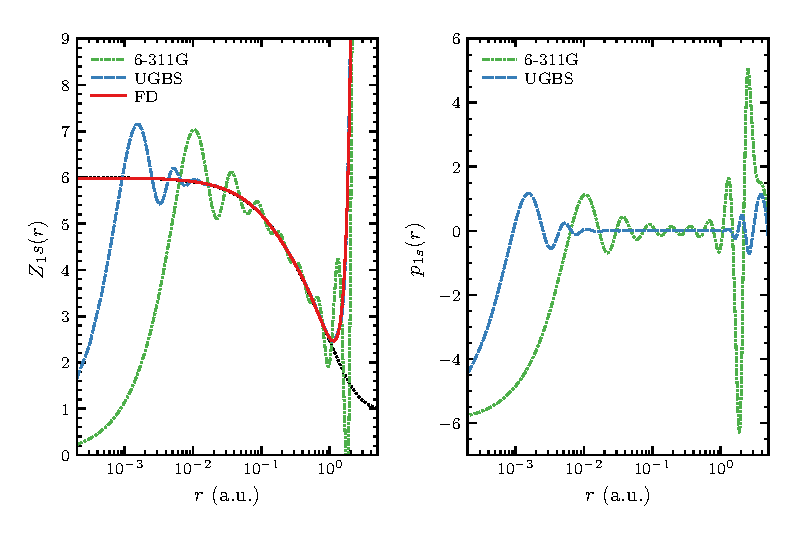
\includegraphics[width=0.9\textwidth]{dim/carbon_prof.eps}
\caption[Inversión de orbitales descritos con conjuntos de base finitos.]
{(a) Cargas efectivas invertidas del orbital $1s$ del átomo de carbón.
(b)~Perfiles de oscilación de los conjuntos de base.}
\label{fig:1sCarbon}
\end{figure}

Para ilustrar este procedimiento, se considera el orbital $1s$ del átomo 
de carbono. Primero, se resuelven las ecuaciones de Hartree--Fock usando 
el conjunto de bases \mbox{6-311G} con el código 
{\sc gamess}~\cite{Schmidt:93,Gordon:05}. Luego, aplicando la 
Ec.~(\ref{eq:Vinv}), se obtiene la carga invertida correspondiente. La 
carga resultante $Z_{1s}^{\mbox{\scriptsize 6-311G}}$ se muestra en la 
Fig.~\ref{fig:1sCarbon}(a) con una línea raya-punto. La carga tiene  
oscilaciones en toda su extensión radial, divergiendo para valores 
grandes de $r$. Se realiza el mismo cálculo con el conjunto de base 
universal gaussiano (\acs{ugbs}), que tiene un número significativamente 
mayor de funciones primitivas. La carga invertida correspondiente 
$Z_{1s}^{\mbox{\scriptsize UGBS}}$ se presenta en la figura con una línea 
discontinua. A pesar que la carga aún diverge cerca de 
$r\approx1\,$a.u., las oscilaciones ahora están circunscriptas cerca del 
núcleo. Finalmente, se resuelven las ecuaciones diferenciales de 
Hartree--Fock para el átomo de carbono usando el método de diferencias 
finitas (\acs{fd}). La carga invertida $Z_{1s}^{\mbox{\scriptsize FD}}$ 
correspondiente se exhibe con una línea sólida en la 
Fig.~\ref{fig:1sCarbon}(a). Como es de esperar, esta carga invertida no 
presenta oscilaciones, ya que no se utilizó una base para construir los 
orbitales. Sin embargo, como se vio en la Sección anterior, la carga 
diverge para $r>1\,$a.u. debido a las características 
de la teoría de Hartree--Fock. En el caso del carbono, los conjuntos de base considerados para 
calcular el orbital $1s$ fueron \mbox{6-311G} y UGBS. Los perfiles de 
oscilación correspondientes, usando la Ec.~(\ref{eq:oscillation-prof}), 
se muestran en la Fig.~\ref{fig:1sCarbon}(b). Dado que los perfiles de 
oscilación para cada conjunto de base atómico son característicos, una 
vez determinados, éstos se pueden implementar para remover las 
oscilaciones de los cálculos moleculares. 


\newpage
%%%%%%%%%%%%%%%%%%%%%%%%%%%%%%%%%%%%%%%%%%%%%%%%%%%%%%%%%%%%%%%%%%%%%%%%
\section{Resultados}
%%%%%%%%%%%%%%%%%%%%%%%%%%%%%%%%%%%%%%%%%%%%%%%%%%%%%%%%%%%%%%%%%%%%%%%%
\label{sec:dimresultados}

En esta Sección se presentan los resultados obtenidos mediante la  
implementación del método de inversión depurada para describir tres 
blancos atómicos (helio, nitrógeno y neón) y sistema molecular (metano). 
El DIM se combina con la primera aproximación de Born para describir la 
ionización por impacto de protones y fotones en estos blancos 
multielectrónicos. Las secciones eficaces de ionización predichas por el 
modelo DIM-FBA se examinan mediante comparación con los datos 
experimentales disponibles.

%%%%%%%%%%%%%%%%%%%%%%%%%%%%%%%%%%%%%%%%%%%%%%%%%%%%%%%%%%%%%%%%%%%%%%%%
\subsection{Estructura electrónica de blancos}
%%%%%%%%%%%%%%%%%%%%%%%%%%%%%%%%%%%%%%%%%%%%%%%%%%%%%%%%%%%%%%%%%%%%%%%%
\label{subsec:dimtarget}

Los orbitales $u_{nl}^{\mathrm{HF}}$ y energías 
$\varepsilon^{\mathrm{HF}}$ de Hartree--Fock que implementamos en la 
Ec.~(\ref{eq:Vinv}) se calculan usando los códigos {\sc hf} de C. F. 
Fischer~\cite{FroeseFischer:97}, y {\sc nrhf} de W. 
Johnson~\cite{Johnson:07}). 
Un aspecto importante en la optimización del potencial está dado por la 
autoconsistencia de los códigos numéricos implementados para el cálculo 
de las soluciones a ser invertidas. Para tal fin, se estudiaron los 
códigos de Hartree--Fock~\cite{FroeseFischer:97,Johnson:07} y se 
implementaron las grillas numéricas específicas de cada código, 
incluyendo los mismos métodos para el cálculo de derivadas. 


%%%%%%%%%%%%%%%%%%%%%%%%%%%%%%%%%%%%%%%%%%%%%%%%%%%%%%%%%%%%%%%%%%%%%%%%
\subsubsection*{Helio}
%%%%%%%%%%%%%%%%%%%%%%%%%%%%%%%%%%%%%%%%%%%%%%%%%%%%%%%%%%%%%%%%%%%%%%%%

En primer lugar, se muestran los resultados obtenidos de implementar
el método de inversión depurada en el átomo de helio en su estado
fundamental. Dado que el orbital $1s$ no tiene nodos y que éste 
decae exponencialmente con la energía del orbital HOMO, la inversión 
directa de este orbital no presenta ninguno de los defectos numéricos
presentados en la Sección~\ref{subsec:invHF}. Además, la simplicidad 
del átomo de helio nos permite ajustar la carga invertida con un número 
reducido de parámetros. La carga invertida $Z_{1s}^{\mathrm{HF}}$ y la
carga invertida depurada $Z_{1s}^{\mathrm{DIM}}$ se muestran en la 
Fig.~\ref{fig:Hepots}(a) con línea discontinua y sólida, 
respectivamente. La carga DIM descrita por la Ec.~(\ref{eq:atomzDIM}), 
se optimiza con sólo tres parámetros, los cuales se dan en la 
Tabla~\ref{tab:params-atoms}. 

\begin{figure}[t]
\centering
\includegraphics[width=0.9\textwidth]{figures/dim/Hepots.eps}
\caption[Cargas efectivas y potencial de intercambio DIM de He.]
{(a) Cargas efectivas $1s$ del He ($^1$S) obtenidas mediante inversión 
directa (línea discontinua) e inversión depurada (línea sólida). 
(b) Potencial de intercambio DIM (línea sólida) y OPM (línea punteada).}
\label{fig:Hepots}
\end{figure}

Para verificar la calidad de la estructura atómica dada por el potencial 
DIM, en la Tabla~\ref{tab:results-atoms} se presenta una comparación 
entre los valores de energías total, orbital y radios medios obtenidos 
utilizando el método de inversión depurada (fila superior) con sus 
correspondientes valores de Hartree--Fock (fila inferior). El potencial 
$V_{1s}^{\mathrm{ DIM}}$ es capaz de producir un valor de energía total, 
dada por la Ec.~\ref{eq:Etotal}, en un $0.003\%$. La energía orbital 
$1s$ coincide con la energía de HF en 6 cifras significativas, mientras 
que los valores medios de $u_{1s}^{\mathrm{DIM}}$ también muestran una 
excelente concordancia, tanto para la región cercana al origen, 
$\langle 1/r\rangle$, como en la región lejana, $\langle r\rangle$.

El potencial de intercambio DIM del átomo de helio, dado por la 
Ec.~\ref{eq:exchange-potential}, se muestra en la 
Fig.~\ref{fig:Hepots}(b). En la figura también se muestran los valores 
OPM, que se obtienen a partir del código \textsc{atomopm} de 
Talman~\cite{Talman:89}, coincide con $V_{1s}^{\mathrm{DIMx}$ en todo 
el rango de $r$. Las energías total y orbital de intercambio, dadas por 
la Ec.~\ref{eq:exchange-energy}, del estado fundamental del helio se 
presentan en la Tabla~\ref{tab:exchange-atoms} y se comparan con el
valor de intercambio exacto de Hartree--Fock (EAHF, por sus siglas en 
inglés) dado por Becke~\cite{Becke:14}.

%%%%%%%%%%%%%%%%%%%%%%%%%%%%%%%%%%%%%%%%%%%%%%%%%%%%%%%%%%%%%%%%%%%%%%%%
\subsubsection*{Nitrógeno}
%%%%%%%%%%%%%%%%%%%%%%%%%%%%%%%%%%%%%%%%%%%%%%%%%%%%%%%%%%%%%%%%%%%%%%%%

Los excelentes resultados obtenidos a partir de la implementación de DIM 
en el átomo de helio pueden atribuirse a la simplicidad del orbital y su 
simetría esférica. Para evaluar la destreza del método de inversión 
depurada para describir blancos con más electrones y de capa abierta, 
se considera ahora el átomo de nitrógeno. 

\begin{figure}[t]
\centering
\includegraphics[width=0.9\textwidth]{figures/dim/N4S_DIM.eps}
\caption[Cargas efectivas DIM de N.]
{Cargas efectivas $1s$, $2s$ y $2p$ del término $^4$S de N obtenidas 
mediante inversión directa (líneas discontinuas) e inversión depurada 
(líneas sólidas).}
\label{fig:Nzeff}
\end{figure}

\begin{figure}[t]
\centering
\includegraphics[width=0.9\textwidth]{figures/dim/N_Vx.eps}
\caption[Potenciales de intercambio DIM de N.]
{Potenciales de intercambio DIM de los términos $^4$S (línea sólida), 
$^2$D (línea discontinua) y $^2$P (línea punto-raya), y valores OPM 
(línea punteada) de N.}
\label{fig:NVx}
\end{figure}

La configuración más baja del nitrógeno $2p^3$ da lugar a tres términos 
diferentes: $^4$S, $^2$D, $^2$P. Cada uno de estos términos está 
descrito por una densidad electrónica diferente. 
En la Fig.~\ref{fig:Nzeff} se muestran las cargas de los orbitales $1s$, 
$2s$ y $2p$ obtenidas a partir de la inversión directa (líneas 
discontinuas) y el método de inversión depurada (líneas continuas) del 
término de energía más bajo de N. Como se vió en la  
Sección~\ref{subsec:invHF}, la inversión del orbital 
$u_{1s}^{\mathrm{HF}}$ diverge en la región asintótica debido a la 
Ec.~\ref{eq:asintoticoVHF}, mientras que el nodo genuino del orbital 
$2s$, en $r\approx 0.32$~a.u., es traducido por la inversión directa 
como un polo a la carga. 

La implementación del método de inversión depurada permite ajustar 
analíticamente la carga invertida en el mayor rango posible. Luego de 
una optimización cuidadosa del blanco, se obtienen los parámetros de las 
cargas DIM correspondientes a los términos $^4$S, $^2$D y $^2$P, que se 
dan en la Tabla~\ref{tab:params-atoms}. Las soluciones que se obtienen 
de la implementación de los potenciales DIM de N se presentan en la 
Tabla~\ref{tab:results-atoms}. Las energías totales, orbitales y valores 
radiales medios se reproducen hasta en un $0.05\%$, $1\times 10^{-4}$ y 
$0.3$ de los valores HF, respectivamente. 

En la Fig.~\ref{fig:NVx} se muestran los potenciales de intercambio 
$1s$, $2s$ y $2p$ de los términos $^4$S (línea sólida), $^2$D (línea 
discontinua) y $^2$P (línea raya-punto) de N. Los potenciales 
$V_{nl}^{\mathrm{DIMx}$ se comparan con el potencial de intercambio OPM
de Talman (línea punteada). Los potenciales de intercambio del orbital 
$1s$ de los términos se comportan de manera similar. El potencial OPM
sigue el comportamiento de estos valores cerca del origen y 
asintóticamente. En el caso del orbital $2s$, los potenciales de 
intercambio correspondientes a cada término se comportan de manera 
diferente en el origen. Para valores $r>0.5$~a.u., los potenciales DIM
y OPM convergen. Nótese que el potencial OPM se comporta como el 
potencial $V_{2s}^{\mathrm{DIMx}$ del término $^2$D concuerda muy bien.
Los potenciales de intercambio DIM $2p$ también se comportan de manera
similar. Sin embargo, los potenciales DIM y OPM convergen sólo en la 
región asintótica. Es notable como el potencial, que no es orbital, 
tiende a seguir el comportamiento de los potenciales orbitales DIM a lo 
largo de $r$. 

Los valores de energía de intercambio orbitales y total de los términos 
$^4$S, $^2$D y $^2$P de N se muestran en la 
Tabla~\ref{tab:exchange-atoms}. La energía de intercambio orbital $1s$ 
de todos los términos son iguales, como se esperaría para un orbital de 
capa cerrada. De manera similar, las energías correspondientes al 
orbital $2s$ varían ligeramente, con una dispersión del $0.08\%$. Sin 
embargo, dado que la capa $2p$ está abierta, la energía de intercambio 
del orbital $2p$ varía significativamente en los diferentes términos, 
con una dispersión de hasta 18\%. Por otro lado, las energías de 
intercambio total, que se obtiene a partir de la 
Ec.~(\ref{eq:exchange-energy}), se comparan con los valores EAHF y 
presentan un acuerdo cercano al $0.1\%$.

%%%%%%%%%%%%%%%%%%%%%%%%%%%%%%%%%%%%%%%%%%%%%%%%%%%%%%%%%%%%%%%%%%%%%%%%
\subsubsection*{Neón}
%%%%%%%%%%%%%%%%%%%%%%%%%%%%%%%%%%%%%%%%%%%%%%%%%%%%%%%%%%%%%%%%%%%%%%%%

La implementación del DIM en neón es análoga al caso de nitrógeno. Esta
vez, la capa de valencia del átomo está llena. Los resultados de la 
optimización de los parámetros que definen las cargas efectivas, dadas 
por la Ec.~(\ref{eq:atomzDIM}), del átomo de neón se muestran en la 
Tabla~\ref{tab:params-atoms}. La comparación entre las soluciones de los 
potenciales DIM y el método de Hartree--Fock se dan en la 
Tabla~\ref{tab:results-atoms}. El acuerdo en energías orbitales es 
excelente, del orden de $1\times 10^{-5}$, mientras que DIM reproduce 
los valores medios de los orbitales HF en aproximadamente $0.1\%$. Por 
otro lado, la energía total tiene una dispersión del $0.04\%$ respecto 
a HF. Las energías de intercambio total y orbitales que se obtienen a 
partir del DIM se presentan en la Tabla~\ref{tab:exchange-atoms}. Las 
energías $E^{\mathrm{x}$ y los valores EAHF acuerdan en $0.04\%$.

%%%%%%%%%%%%%% RESULTADOS %%%%%%%%%%%%%%
\begin{table}
\begin{center}
\begin{tabularx}{\textwidth}{
>{\centering\arraybackslash}p{0.12\textwidth}
>{\centering\arraybackslash}p{0.05\textwidth}
>{\centering\arraybackslash}p{0.22\textwidth}
>{\centering\arraybackslash}p{0.22\textwidth}
>{\centering\arraybackslash}p{0.22\textwidth}}
\rowcolor{mydarkgray} 
   &       & $nl$ & $z_j$        & $\alpha_j$   \\
%%%%%%%%%%%%%%%%%%%% Helio %%%%%%%%%%%%%%%%%%%%
He & $^1$S & $1s$ &  $1.3175$ & $2.5003$  \\\rowcolor{mygray} 
   &       &      & $-0.3175$ & $5.0437$  \\ 
%%%%%%%%%%%%%%%%%% Nitrogeno %%%%%%%%%%%%%%%%%%
N  & $^4$S & $1s$ & $5.2563$ & $1.2621$  \\\rowcolor{mygray} 
   &       &      & $0.7437$ & $8.0284$  \\ 
   &       & $2s$ & $2.7136$ & $0.8947$ \\\rowcolor{mygray} 
   &       &      & $2.4528$ & $3.5127$  \\
   &       &      & $0.8336$ & $3.3865$  \\ \rowcolor{mygray} 
   &       & $2p$ & $3.6435$ & $1.2407$  \\ 
   &       &      & $2.0550$ & $5.3514$  \\\rowcolor{mygray} 
   &       &      & $0.3015$ & $0.2866$ \\
   & $^2$D & $1s$ & $5.1664$ & $1.2241$  \\\rowcolor{mygray} 
   &       &      & $0.8137$ & $7.5680$  \\ 
   &       & $2s$ & $3.7478$ & $2.8531$  \\\rowcolor{mygray} 
   &       &      & $1.8541$ & $1.0311$  \\ 
   &       &      & $0.3981$ & $0.2397$ \\\rowcolor{mygray} 
   &       & $2p$ & $4.0105$ & $1.2874$  \\ 
   &       &      & $1.8552$ & $5.7086$  \\\rowcolor{mygray} 
   &       &      & $0.1343$ & $0.2680$ \\
   & $^2$P & $1s$ & $5.1864$ & $1.2178$  \\\rowcolor{mygray} 
   &       &      & $0.8137$ & $7.5674$  \\ 
   &       & $2s$ & $3.6700$ & $3.1495$  \\\rowcolor{mygray} 
   &       &      & $1.4394$ & $0.7404$  \\ 
   &       &      & $0.8907$ & $0.8306$ \\\rowcolor{mygray} 
   &       & $2p$ & $2.3280$ & $1.4093$  \\ 
   &       &      & $1.8977$ & $1.1656$  \\\rowcolor{mygray} 
   &       &      & $1.7743$ & $5.6878$ \\
%%%%%%%%%%%%%%%%%%%%%%%%%%%%%%%%%%%%%%%%%%%%%%%
Ne & $^1$S & $1s$ & $7.3677$ & $2.4173$ \\\rowcolor{mygray} 
   &       &      & $1.3004$ & $0.1264$ \\
   &       &      & $0.3320$ & $13.1582$ \\\rowcolor{mygray} 
   &       & $2s$ & $0.2977$ & $17.9939$ \\
   &       &      & $0.6681$ & $0.0673$ \\\rowcolor{mygray} 
   &       &      & $8.0342$ & $2.4722$ \\
   &       & $2p$ & $1.3531$ & $8.5695$ \\\rowcolor{mygray} 
   &       &      & $0.3359$ & $0.4649$ \\
   &       &      & $7.3111$ & $2.0906$ \\
\end{tabularx}
\caption[Parámetros de la carga efectiva de He, N y Ne.]
{Parámetros de la carga efectiva $Z_{1s}^{\mathrm{ DIM}}$ de He ($^1$S), 
N ($^4$S, $^2$D, $^2$P) y Ne ($^1$S).}
\label{tab:params-atoms}
\end{center}
\end{table}

\begin{table}
\begin{center}
\begin{tabularx}{\textwidth}{
>{\centering\arraybackslash}p{0.07\textwidth}
>{\centering\arraybackslash}p{0.03\textwidth}
>{\centering\arraybackslash}p{0.15\textwidth}
>{\centering\arraybackslash}p{0.10\textwidth}
>{\centering\arraybackslash}p{0.15\textwidth}
>{\centering\arraybackslash}p{0.15\textwidth}
>{\centering\arraybackslash}p{0.15\textwidth}}
\rowcolor{mydarkgray} 
   & & $E$ & $nl$ & $\varepsilon_{nl}$ & $\left<r\right>_{nl}$ & $\left<1/r\right>_{nl}$ \\
He & $^1$S & $-2.8616$   & $1s$ & $-0.9180$  & $0.9273$ & $1.6873$ \\\rowcolor{mygray} 
   &       & $-2.8617$   &      & $-0.9180$  & $0.9273$ & $1.6873$ \\
N  & $^4$S & $-54.3762$  & $1s$ & $-15.6291$ & $0.2283$ & $6.6487$ \\\rowcolor{mygray} 
   &       & $-54.4009$  &      & $-15.6291$ & $0.2283$ & $6.6532$ \\
   &       &             & $2s$ & $-0.9453$  & $1.3345$ & $1.0804$ \\\rowcolor{mygray} 
   &       &             &      & $-0.9453$  & $1.3323$ & $1.0782$ \\
   &       &             & $2p$ & $-0.5676$  & $1.4127$ & $0.9550$ \\\rowcolor{mygray} 
   &       &             &      & $-0.5676$  & $1.4096$ & $0.9577$ \\
   & $^2$D & $-54.2756$  & $1s$ & $-15.6664$ & $0.2283$ & $6.6493$ \\\rowcolor{mygray} 
   &       & $-54.2962$  &      & $-15.6664$ & $0.2283$ & $6.6539$ \\
   &       &             & $2s$ & $-0.9637$  & $1.3292$ & $1.0874$ \\\rowcolor{mygray} 
   &       &             &      & $-0.9637$  & $1.3263$ & $1.0832$ \\
   &       &             & $2p$ & $-0.5087$  & $1.4488$ & $0.9388$ \\\rowcolor{mygray} 
   &       &             &      & $-0.5087$  & $1.4466$ & $0.9421$ \\
   & $^2$P & $-54.2086$  & $1s$ & $-15.6916$ & $0.2282$ & $6.6504$ \\\rowcolor{mygray} 
   &       & $-54.2281$  &      & $-15.6916$ & $0.2282$ & $6.6543$ \\
   &       &             & $2s$ & $-0.9763$  & $1.3256$ & $1.0871$ \\\rowcolor{mygray} 
   &       &             &      & $-0.9763$  & $1.3223$ & $1.0866$ \\
   &       &             & $2p$ & $-0.4713$  & $1.4718$ & $0.9298$ \\\rowcolor{mygray} 
   &       &             &      & $-0.4713$  & $1.4730$ & $0.9316$ \\
Ne & $^1$S & $-128.4978$ & $1s$ & $-32.7725$ & $0.1575$ & $9.6215$ \\\rowcolor{mygray} 
   &       & $-128.5475$ &      & $-32.7724$ & $0.1576$ & $9.6181$ \\
   &       &             & $2s$ & $-1.9304$  & $0.8913$ & $1.6408$ \\\rowcolor{mygray} 
   &       &             &      & $-1.9304$  & $0.8921$ & $1.6326$ \\  
   &       &             & $2p$ & $-0.8504$  & $0.9678$ & $1.4303$ \\\rowcolor{mygray} 
   &       &             &      & $-0.8504$  & $0.9653$ & $1.4354$ \\
\end{tabularx}
\caption[Energías y radios medios de He, N y Ne.]
{Energías totales, energías orbitales y radios medios de He ($^1$S), 
N ($^4$S, $^2$D, $^2$P) y Ne ($^1$S) obtenidos con el método de 
inversión depurada (filas superiores) y con el método de HF (filas 
inferiores).}
\label{tab:results-atoms}
\end{center}
\end{table}

\begin{table}
\begin{center}
\begin{tabularx}{\textwidth}{
>{\centering\arraybackslash}p{0.07\textwidth}
>{\centering\arraybackslash}p{0.03\textwidth}
>{\centering\arraybackslash}p{0.14\textwidth}
>{\centering\arraybackslash}p{0.14\textwidth}
>{\centering\arraybackslash}p{0.14\textwidth}
>{\centering\arraybackslash}p{0.14\textwidth}
>{\centering\arraybackslash}p{0.14\textwidth}}
\rowcolor{mydarkgray} 
   &      & $1s$     & $2s$     & $3s$     & Total    & EAHF~\cite{Becke:14} \\
He & $^1$S & $-0.5129$ &           &           & $-1.0258$ & $-1.026$ \\\rowcolor{mygray} 
N  & $^4$S & $-2.1175$ & $-0.4776$ & $-0.4711$ & $-6.6034$ & $-6.596$ \\
   & $^2$D & $-2.1175$ & $-0.4777$ & $-0.4262$ & $-6.4688$ & \\\rowcolor{mygray} 
   & $^2$P & $-2.1175$ & $-0.4780$ & $-0.3973$ & $-6.3827$ & \\
Ne & $^1$S & $-3.1106$ & $-0.8620$ & $-0.6938$ & $-12.1080$ & $-12.105$ \\\rowcolor{mygray} 
\end{tabularx}
\caption[Energías de intercambio total y orbitales de He, N y Ne.]
{Energías de intercambio total y orbitales DIM de He ($^1$S), N ($^4$S, 
$^2$D, $^2$P) y Ne ($^1$S).}
\label{tab:exchange-atoms}
\end{center}
\end{table}

\newpage
%%%%%%%%%%%%%%%%%%%%%%%%%%%%%%%%%%%%%%%%%%%%%%%%%%%%%%%%%%%%%%%%%%%%%%%%
\subsubsection*{Metano}
%%%%%%%%%%%%%%%%%%%%%%%%%%%%%%%%%%%%%%%%%%%%%%%%%%%%%%%%%%%%%%%%%%%%%%%%

El método de inversión depurada para sistemas moleculares se aplica a 
la molécula de metano. Este hidruro es altamente simétrico y, por lo 
tanto, puede ser descrito por un potencial angular 
promediado~\cite{Granados:16}. 

\begin{figure}[t]
\centering
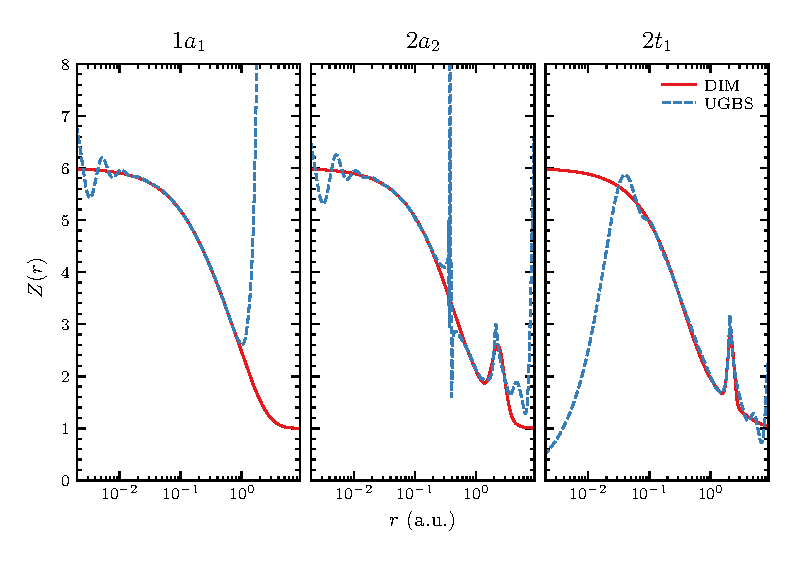
\includegraphics[width=0.9\textwidth]{figures/dim/ch4_dim.eps}
\caption[Cargas invertidas y depuradas de metano.]
{Cargas efectivas de CH$_4$ de los orbitales moleculares $1a_1$, $2a_2$ 
y $2t_1$ obtenidas a partir del conjunto de base UGBS; inversión directa 
(líneas discontinuas) e inversión depurada (líneas sólidas).}
\label{fig:ch4zeff}
\end{figure}

% ver si incluir una frase sobre la expansión de un centro de los orbitales moleculares multicentricos
Los orbitales moleculares HF de CH$_4$ se calculan usando los conjuntos 
de bases UGBS del carbono y el hidrógeno. Estas bases sólo consideran 
momentos angulares hasta $L=1$. El cálculo de estructura electrónica de 
metano con estos conjuntos de base deberían incluir funciones de 
polarización (por lo menos hasta las funciones $d$), con el fin de 
incrementar la precisión de las energías moleculares~\cite{Rothenberg:71,
Hariharan:72}. Sin embargo, para aislar los efectos de la base, los 
cálculos de perfiles de oscilación descritos en la 
Sección~\ref{sec:dimmoleculas} y los orbitales moleculares se realizan 
en el mismo esquema. Las cargas obtenidas mediante la inversión directa 
de estos orbitales se muestran en la Fig.~\ref{fig:ch4zeff} con líneas 
discontinuas. Dado que los orbitales moleculares están escritos por 
combinaciones lineales de orbitales atómicos del carbono y el hidrógeno, 
las oscilaciones de las cargas invertidas se deben al número finito de 
funciones primitivas en el conjunto de base de cada átomo. Para remover 
estas oscilaciones, se deben determinar los perfiles de oscilación 
producidas por la base de los átomos constituyentes. Se emplea la 
Ec.~(\ref{eq:oscillation-prof}) para determinar los perfiles 
$p_{1s}^{\mbox{\scriptsize UGBS}}$, $p_{2s}^{\mbox{\scriptsize UGBS}}$ y 
$p_{2p}^{\mbox{\scriptsize UGBS}}$ del carbono. Así, se puden remover 
los perfiles $p_{nl}^{\mbox{\scriptsize UGBS}}$ de las correspondientes 
cargas invertidas $Z_{nl}^{\mbox{\scriptsize UGBS}}$ del metano. Las 
oscilaciones se remueven completamente para todos los orbitales excepto 
el $2a_2$, que presenta pequeñas fluctuaciones residuales debido a la 
base del hidrógeno. Ya que estas ondulaciones son mínimas y se ubican 
cerca del núcleo, éstas pueden ser despreciadas y se procede a 
implementar el método de depuración descrito en la 
Sección~\ref{sec:dimmoleculas}. 

Los parámetros optimizados de las cargas moleculares DIM, dadas por la 
Ec.~(\ref{eq:molzDIM}), se presentan en la Tabla~\ref{tab:ch4parameters}. 
Las cargas correspondientes se muestran en la Fig.~\ref{fig:ch4zeff} con 
líneas sólidas. En este caso, para la construcción de función de 
costo~(\ref{eq:fncosto-dim}) que se miniza considera los valores de 
energía y radios medios de los MOs dados por Moccia~\cite{Moccia:69}. 
las energías orbitales reproducen las originales hasta la cuarta cifra 
significativa y se dan en la Tabla~\ref{tab:ch4parameters}. Por otro 
lado, los radios medios $\langle r\rangle$ y $\langle 1/r\rangle$ 
obtenidos con los potenciales moleculares DIM están dentro del $1\%$ 
de los valores de Moccia.

\begin{table}[t]
\centering
\begin{tabular}{
>{\centering\arraybackslash}p{0.13\textwidth}
>{\centering\arraybackslash}p{0.13\textwidth}
>{\centering\arraybackslash}p{0.13\textwidth}
>{\centering\arraybackslash}p{0.13\textwidth}
>{\centering\arraybackslash}p{0.13\textwidth}
>{\centering\arraybackslash}p{0.13\textwidth}}
\rowcolor{mydarkgray} 
   $nl$ & $E$        & $z$        & $\alpha$   & $\beta$ & $\gamma$ \\
$1a_1$  & $-11.1949$ & $1.925280$ & $0.641982$ & & \\
\rowcolor{mygray} 
        &            & $0.953120$ & $5.571510$ & & \\
        &            & $2.121600$ & $1.500440$ & & \\
\rowcolor{mygray} 
$2a_2$  & $-0.9204$  & $2.912200$ & $3.149990$ & & \\
        &            & $2.087800$ & $0.771371$ & & \\
\rowcolor{mygray} 
        &            & $1.23640$  &            & $2.329570$ & $0.053420$ \\
$2t_1$  & $-0.5042$  & $0.901953$ & $2.895140$ & & \\
\rowcolor{mygray} 
        &            & $1.112030$ & $0.388649$ & & \\
        &            & $2.986017$ & $2.931210$ & & \\
\rowcolor{mygray} 
        &            & $1.301820$ &            & $2.169850$ & $0.012616$ \\ 
\end{tabular}
\caption[Energías y parámetros de ajuste de cargas efectivas de metano.]
{Energías orbitales moleculares y parámetros de ajuste de cargas 
efectivas de metano.}
\label{tab:ch4parameters}
\end{table}

%%%%%%%%%%%%%%%%%%%%%%%%%%%%%%%%%%%%%%%%%%%%%%%%%%%%%%%%%%%%%%%%%%%%%%%%
\subsection{Procesos colisionales simples}
%%%%%%%%%%%%%%%%%%%%%%%%%%%%%%%%%%%%%%%%%%%%%%%%%%%%%%%%%%%%%%%%%%%%%%%%
\label{subsec:procol}

En esta Sección se analiza la respuesta de los potenciales efectivos 
DIM obtenidos en la Sección~\ref{subsec:dimtarget} mediante el método 
de inversión depurada para helio, nitrógeno, neón y metano.
En los blancos moleculares, la orientación molecular es importante para 
determinar la sección eficaz en un proceso colisional. Sin embargo, en 
sistemas gasesosos, las moléculas tienen orientaciones aleatorias que no 
están predefinidas en el experimento. Por lo tanto, la descripción 
promediada esféricamente de los sistemas moleculares asumida por el 
potencial DIM está en concordancia con la configuración del blanco.
Los procesos colisionales que se examinan en esta Sección se describen a 
primer orden empleando la primera aproximación de Born (FBA). 
La combinación de la descripción del blanco mediante el potencial 
efectivo DIM y el modelado de la fotoionización a primer orden se 
denomina como ionización DIM-FBA. 

%%%%%%%%%%%%%%%%%%%%%%%%%%%%%%%%%%%%%%%%%%%%%%%%%%%%%%%%%%%%%%%%%%%%%%%%
\subsubsection{Fotoionización}
%%%%%%%%%%%%%%%%%%%%%%%%%%%%%%%%%%%%%%%%%%%%%%%%%%%%%%%%%%%%%%%%%%%%%%%%
\label{subsec:foto}

Las secciones eficaces de ionización simple por impacto de fotón según 
el modelo DIM-FBA para helio, nitrógeno, neón y metano se muestran en 
la Fig.~\ref{fig:photoDIM} con líneas sólidas. Los resultados teóricos 
DIM-FBA para helio y nitrógeno coinciden de manera excelente con los 
valores experimentales (símbolos)~\cite{Samson:90,Henke:93,Stolte:16} a 
bajas, medias y altas energías del fotón incidente. En el caso del átomo 
de neón, algunas discrepancias con las mediciones (símbolos) 
\cite{Henke:93,Samson:02} empiezan a surgir a energías bajas e 
intermedias del projectil. Este comportamiento sugiere la necesidad de 
incluir en la descripción de la fotoionización correcciones de mayor 
orden que incluyan efectos de múltiples cuerpos que puedan ser 
relevantes, tales como la relajación de los orbitales debido a la 
creación de un hueco electrónico, respuestas colectivas de electrones 
de capas internas~\cite{Ederer:64} y efectos de correlación.

\begin{figure}
\centering
\includegraphics[width=0.92\textwidth]{dim/fotoDIM-part1.eps} 

\vspace{-1.15cm}
\includegraphics[width=0.92\textwidth]{dim/fotoDIM-part2.eps}
\caption[Fotoionización de He, N, Ne y CH$_4$.]
{Sección eficaz total de fotoionización de un electrón de He~$^1$S, 
N~$^4$S, Ne~$^1$S y CH$_4$. Curvas: cálculos teóricos DIM-FBA. Símbolos: 
datos experimentales~\cite{Samson:90,Henke:93,Stolte:16,Samson:02,
Lukirskii:64,Henke:82,Samson:89}.}
\label{fig:photoDIM}
\end{figure}

La predicción del modelo DIM-FBA para la sección eficaz total de 
fotonización de CH$_4$ se encuentra en buen acuerdo con valores 
experimentales en el rango de altas energías y cerca del umbral. La 
curva entre aproximadamente 15 y 300 eV muestra la fotoionización de la 
capa eterna $n=2$, mientras que la discontinuidad en $0.3$~keV 
corresponde al umbral del orbital molecular $1a_1$. Para fotoenergías 
bajas e intermedias, el acuerdo entre las predicciones DIM-FBA y los 
datos experimentales~\cite{Lukirskii:64,Henke:82,Samson:89} no es bueno. 
Fenónemos tales como la relajación de los orbitales moleculares, 
posibles contribuciones colectivas y efectos de correlación deben ser  
considerados en futuros cálculos. Por otro lado, para la fotoionización 
de un electrón perteneciente al orbital interno $1a_1$, estos efectos no 
son tan signficativos, y se tiene buen acuerdo con los valores 
experimentales disponibles. 

%=======================================================================
\subsubsection{Ionización por impacto de iones}
\label{subsec:dimion}

\begin{figure}
\centering
\includegraphics[width=0.9\textwidth]{figures/dim/ionDIM.eps}
\caption[Ionización por impacto de protón de N y CH$_4$.]
{Sección eficaz total de ionización de un electrón por impacto de protón 
de N~$^4$S y CH$_4$. Línea sólida: cálculos teóricos DIM-FBA. 
Símbolos: datos experimentales de ionización por impacto de 
protón~\cite{Rudd:83,Rudd:85} y electrón~\cite{Brook:78} con conversión 
de equivelocidad.}
\label{fig:iondim}
\end{figure}

Los resultados de ionización por impacto de protón en N~$^4$S y CH$_4$, 
en el marco del modelo DIM-FBA, se muestra en la Fig.~\ref{fig:iondim}. 
El acuerdo entre las predicciones teóricas y las datos experimentales es 
muy bueno en la región de altas energías, donde tiene validez la primera 
aproximación de Born. En el caso de nitrógeno, incluimos también datos 
experimentales de ionización por impacto de electrón. Para valores de 
energía mayores a 400~keV, se espera que la sección eficaz de ambos 
proyectiles coincida. 

%=======================================================================
\section{Conclusiones}
\label{conclusion}

En este Capítulo se desarrolló el método de inversión depurada (DIM) 
para obtener potenciales efectivos que permitan describir la estructura 
electrónica de blancos atómicos y moleculares de manera precisa. La 
disponibilidad de estos potenciales permite conocer los estados 
iniciales y finales del blanco en una colisión de manera directa. 

Los potenciales DIM se obtienen a partir de la inversión de ecuaciones 
de un electrón con soluciones de Hartree--Fock. Los potenciales 
resultantes presentan defectos numéricos (polos y divergencias), los 
cuales son examinados en detalle. Se encuentra que los defectos están 
dados por características de la teoría de Hartree--Fock no compatibles
con la inversión. Los polos se deben a nodos genuinos de los orbitales 
HF que no son puntos de inflexión. Si bien esta característica de los 
orbitales no es explícita en la teoría, la obtención de potenciales sin 
polos así lo requiere. Las divergencias asintóticas del potencial se 
deben al coeficiente del decaimiento exponencial de los orbitales HF. 
La teoría de HF establece que éstos decaen con la energía del HOMO. Sin 
embargo, la obtención de potenciales con correcto comportamiento 
asintótico mediante el esquema de inversión requiere que cada orbital 
decaiga con la energía del dicho orbital. También se encontraron 
oscilaciones en los orbitales de las capas internas de átomos con carga 
nuclear $Z\ge 12$, que dan lugar a nodos espurios. Estas oscilaciones 
parecen surgir debido al término de intercambio a grandes distancias. 
Para tratar los defectos encontrados en la inversión, se desarrolló el 
método de depuración, que consiste en ajustar las cargas invertidas, en 
regiones sin polos ni divergencias, mediante una expresión analítica. 
Los parámetros que definen esta expresión son optimizados cuidadosamente 
hasta reproducir las soluciones iniciales.

El método de inversión depurada para átomos fue extendido para 
moléculas. Debido a que los orbitales moleculares se expresan a partir 
de conjuntos de base finitas, las soluciones presentan ondulaciones casi 
imperceptiles. La implementación de la inversión traduce estas pequeñas 
fluctuaciones como grandes oscilaciones en la carga molecular. Debido a 
esto, se requieren pasos adicionales en el método de depuración, los 
cuales incluyen la determinación de perfiles de oscilación de los 
conjuntos de base atómicas utilizadas en el cálculo molecular. 

Dado que la teoría de Hartree--Fock contiene el término de intercambio
de forma exacta, a partir de los potenciales DIM, se definió una 
expresión que permite determinar potenciales de intercambio orbitales 
``exactos'' de manera simple. A su vez, estos potenciales se emplean 
para definir energías de intercambio orbitales y totales.

Se implementó el método DIM para obtener potenciales efectivos y de 
intercambio que reproducen las soluciones de HF de forma precisa en tres 
blancos atómicos: helio, nitrógeno y neón. Además, se empleó el método 
DIM extendido a moléculas para describir la molécula de metano. Las 
soluciones que se obtienen de estos potenciales reproducen los valores
originales con gran precisión. 

La efectividad del DIM para describir la estructura de blancos en una 
colisión fue examinado a partir de la primera aproximación de Born. Los 
potenciales de He, N, Ne y CH$_4$ se implementaron para calcular, en 
conjunción con la FBA, secciones eficaces de ionización por el impacto 
de protones y fotones. En términos generales, ambos procesos se 
reproducen con buena concordancia los datos experimentales disponibles. 
Las discrepancias principales se atribuyen al hecho de que el modelo 
teórico sólo considera el primer orden perturbativo. Será necesario 
implementar métodos perturbativos con mayor orden de aproximación para 
examinar la validez del método DIM en la región de energías intermedias.


%%%%%%%%%%%%%%%%%%%%%%%%%%%%%%%%%%%%%%%%%%%%%%%%%%%%%%%%%%%%%%%%%%%%%%%%
\section{Discusión: DIM como instancia superadora de HF?}
%%%%%%%%%%%%%%%%%%%%%%%%%%%%%%%%%%%%%%%%%%%%%%%%%%%%%%%%%%%%%%%%%%%%%%%%
\label{sec:discusion}

%%% Fallas
%%% Nodos que no son puntos de inflexión  -> Derivada 2da
%%% Nodos que son espurio (no localidad) -> Fischer
%%% Divergencia a grandes r               -> Hartree

% Defectos: 
% Los defectos de las cargas invertidas surgen del propio método de Hartree--Fock; los nodos genuinos no son estrictamente puntos de  inflexión, el decaimiento exponencial de los orbitales sigue el comportamiento orbitales tipo Hartree, mientras que el método autoconsistente conduce a la aparición de nodos espurios.

En general, las cargas resultantes de la inversión de los orbitales HF 
tienen asociadas alguno de estos defectos. A partir de dos ejemplos, 
se examina cada uno de ellos y su transfondo téorico a través un 
experimento numérico. Sin embargo, el análisis se puede generalizar 
para los orbitales HF de cualquier átomo no relativista.

%%%%%%%%%%%%%%%%%%%%%%%%%%%%%%%%%%%%%%%%%%%%%%%%%%%%%%%%%%%%%%%%%%%%%%%%
\subsubsection*{Nodos genuinos}
%%%%%%%%%%%%%%%%%%%%%%%%%%%%%%%%%%%%%%%%%%%%%%%%%%%%%%%%%%%%%%%%%%%%%%%%

En la Fig.~\ref{fig:example2sMg} se muestra la función 
$u_{2s}^{\mathrm{HF}}$ del Mg y su derivada segunda numérica (escalada 
por un factor). Las dos raices de $u_{2s}^{\mathrm{HF}}''$ son puntos de 
inflexión de $u_{2s}^{\mathrm{HF}}$ y se corresponden a (1)~el nodo 
genuino y (2)~el punto de inflexión clásico. A primera vista, el nodo 
genuino y el primer punto de inflexión parecen coincidir. Sin embargo, 
una inspección más cercana (ver recuadro) muestra que ese no es el caso. 
Definiendo $\Delta r$ como la distancia entre el nodo del orbital y la 
primera raiz de su derivada segunda, se encuentra una pequeña distancia 
$\Delta r=1\times 10^{-3}$~a.u. entre las primeras raices de ambas 
funciones. Si bien no existe ninguna restricción en la teoría que fuerce 
a los nodos genuinos de HF a ser también puntos de inflexión, este 
fenómeno es sistemático en todos los orbitales HF con nodos de los 
átomos con $Z\ge 12$.

\begin{figure}
\vspace{-0.4cm}
\centering
\includegraphics[width=0.85\textwidth]{dim/example_2sMg.eps} 
\vspace{-0.45cm}
\caption[Orbital radial y su derivada segunda.]
{Orbital radial $u_{2s}^{\mathrm{HF}}$ del estado fundamental de Mg y su 
derivada segunda escalada.}
\label{fig:example2sMg}
%\end{figure}

\vspace{0.4cm}
%\begin{figure}
%\centering
\includegraphics[width=0.85\textwidth]{dim/dr_2sMg.eps} 
\vspace{-0.45cm}
\caption[Dependecia de $\Delta r$ del orden de aproximación numérica.]
{Dependecia de $\Delta r$ del orden de aproximación numérica en el 
orbital $2s$ del átomo de potasio. (a) Primer orden y 200 puntos, (b) 
400 puntos; (c) octavo orden y 1000 puntos.}
\label{fig:dr2sMg}
\end{figure}

Estos hallazgos permiten suponer que la cercanía entre los nodos 
genuinos de los orbitales y las correspondientes raices de su segunda 
derivada no es casual, y que los nodos genuinos en la teoría de 
Hartree--Fock deben ser puntos de inflexión. El experimento numérico 
que se diseña para indagar esta hipótesis consiste en realizar varias 
aproximaciones con mejoras sucesivas en su precisión, examinando el 
comportamiento del valor $\Delta r$ resultante. La calidad de los 
métodos numéricos usados para resolver las ecuaciones de HF se evalúan 
variando el orden de precisión de los algoritmos y la densidad de puntos 
de las grillas numéricas. En este experimento se utiliza el método 
lineal de pasos múltiples de Adams--Moulton para las ecuaciones 
diferenciales y el método de diferenciación Lagrangiana para las 
derivadas. La metodología propuesta se implementa modificando el código 
\textsc{nrhf} de Johnson~\cite{Johnson:07}, que usa aproximaciones de 
octavo orden por defecto. %No obstante, los mismos resultados y 
%conclusiones se obtienen con el código~\textsc{hf} de 
%Fischer~\cite{FroeseFischer:97}.

La Fig.~\ref{fig:dr2sMg} muestra $u_{2s}^{\mathrm{HF}}$ de Mg (línea 
sólida) y su segunda derivada numérica (línea discontinua) en las 
proximidades del nodo implementando tres grados de aproximación 
distintos en los métodos numéricos. Los cálculos menos precisos se 
muestran en la Fig.~\ref{fig:dr2sMg}(a), donde se implementa el primer 
orden de los algoritmos numéricos y una grilla numérica de 200 puntos 
(mínimo valor necesario para obtener convergencia), resultando en 
$\Delta r=8\times 10^{-3}$~a.u.. Aumentando el número de puntos a 400, 
este valor se reduce a $\Delta r=4\times 10^{-3}$~a.u., como se muestra 
en la Fig.~\ref{fig:dr2sMg}(b). Por último, se incrementa el número de 
puntos a 1000 y se usa el máximo orden de aproximación de los 
algoritmos. La Fig.~\ref{fig:dr2sMg}(c) muestra el mejor resultado 
posible, donde $\Delta r=1\times 10^{-3}$~a.u.. Aún considerando un 
número mayor de puntos en la grilla numérica, los resultados no varían. 
Se realizó un cálculo adicional usando el método del potencial efectivo 
optimizado (\acs{oep}) desarrollado por Talman~\cite{Sharp:53,Talman:76,
Talman:89}. La Fig.~\ref{fig:dr2sMg}(c) muestra el orbital 
$u_{2s}^{\mathrm{OEP}}$ de Mg cerca del nodo con una línea raya-punto. 
Debido al caracter local del potencial, su segunda derivada 
$u_{2s}^{\mathrm{OEP}}''$ (línea punto-raya-punto) es estrictamente cero 
en el nodo. 

Es posible que la no localidad del método de Hartree--Fock sea 
responsable de que los nodos genuinos en los orbitales no sean puntos de 
inflexión. Una exploración más en detalle, con mayores órdenes de 
aproximación en los métodos numéricos, será necesaria para descartar 
esta hipótesis. La excelente reproducción de los orbitales HF mediante 
el potencial local OEP parece sugerir que esta premisa es correcta. De 
ser el caso, se podría agregar una restricción adicional al 
procedimiento variacional autoconsistente de Hartree--Fock. En 
definitiva, el cumplimiento de esta restricción aseguraría un potencial 
local, en principio, sin polos.

%%%%%%%%%%%%%%%%%%%%%%%%%%%%%%%%%%%%%%%%%%%%%%%%%%%%%%%%%%%%%%%%%%%%%%%%
\subsubsection*{Decaimiento exponencial}
%%%%%%%%%%%%%%%%%%%%%%%%%%%%%%%%%%%%%%%%%%%%%%%%%%%%%%%%%%%%%%%%%%%%%%%%

Los orbitales de los electrones ligados decaen exponencialmente para 
distancias mayores al punto de retorno clásico. A grandes distancias 
$r$, el decaimiento asintótico de la parte radial de los orbitales HF 
está determinado por la energía del orbital molecular de mayor ocupación 
(\acs{homo}) $\varepsilon_{\mathrm{HOMO}}^{\mathrm{HF}}$ 
\cite{Handy:69,Handler:80,Ishida:92}},
\begin{equation}
\lim_{r \rightarrow \infty} u_{nl}^{\mathrm{HF}}(r) =  
\exp(- \sqrt{- 2 \varepsilon_{\mathrm{HOMO}}^{\mathrm{HF}} } r )  \, .
\label{eq:rHF}
\end{equation}
Por otro lado, los orbitales que corresponden a potenciales esféricos 
tienen un decaimiento asintótico de tipo Hartree~\cite{Casida:89},
\begin{equation}
\lim_{r \rightarrow \infty} u_{nl}^{\mathrm{DIM}}(r) =  
\exp(- \sqrt{- 2 \varepsilon_{nl}^{\mathrm{HF}} } r ) \,.
\label{eq:rHlike}
\end{equation}
El término ``tipo-Hartree'' puede resultar confuso ya que la energía 
del orbital $\varepsilon_{nl}^{\mathrm{HF}}$ se corresponde a valores 
donde se ha considerado el término de intercambio. El comportamiento 
asintótico de los orbitales HF se puede examinar en detalle a través de 
la derivada logaritmica de los orbitales radiales, 
\begin{equation}
L_{nl}(r) \equiv r \frac{d \log{u_{nl}}}{d r}\,,
\label{eq:Lnl}
\end{equation}
que se comporta de forma lineal para funciones $u_{nl}$ que decaen 
exponencialmente. 

\begin{figure}[t]
\centering
\includegraphics[width=0.9\textwidth]{dim/Lns_K.eps} 
\caption[Comportamiento asintótico de los orbitales HF.]
{Comportamiento asintótico de los orbitales HF según $L_{nl}$, dada por 
la Ec.~\ref{eq:Lnl}, de los orbitales $s$ del átomo de K.}
\label{fig:LnsK}
\end{figure}

La Fig.~\ref{fig:LnsK} muestra la derivada logarítmica de los orbitales 
HF $ns$ del átomo de potasio. Los orbitales HF se presentan con líneas 
discontinuas (capas internas) y sólidas (capa de valencia). A grandes 
distancias, los orbitales presentan el comportamiento de Hartree--Fock 
dado por la Ec.~\ref{eq:rHF}: los orbitales de las capas internas siguen 
el decaimiento asintótico del \acs{homo}. Además, se incluye el 
comportamiento de tipo Hartree correspondiente a cada orbital (líneas 
punteadas). Se observa que las funciones $u_{nl}^{\mathrm{HF}}$ tienen 
este decaimiento exponencial a partir del punto de retorno clásico de 
cada orbital y hasta $0.4$~a.u., $1.5$~a.u. y 5~a.u. en los orbitales 
$1s$, $2s$ y $3s$, respectivamente. 
En este caso, el comportamiento asintótico del potencial 
invertido~(\ref{eq:VHF}) correspondiente a los orbitales está dado por
\begin{equation}
\lim_{r \rightarrow \infty} V_{ns}^{\mathrm{HF}}(r)=
-\left(\varepsilon_{\mathrm{HOMO}}^{\mathrm{HF}}
-\varepsilon_{ns}^{\mathrm{HF}}\right) \,,
\label{eq:asintoticoVHF}
\end{equation}
que es siempre distinto de cero, excepto para el \acs{homo}. Así, como 
se había anticipado, las divergencias en las cargas invertidas se deben 
al coeficiente del término exponencial de $u_{nl}(r)$ a grandes 
distancias. 

%%%%%%%%%%%%%%%%%%%%%%%%%%%%%%%%%%%%%%%%%%%%%%%%%%%%%%%%%%%%%%%%%%%%%%%%
\subsubsection*{Nodos espurios}
%%%%%%%%%%%%%%%%%%%%%%%%%%%%%%%%%%%%%%%%%%%%%%%%%%%%%%%%%%%%%%%%%%%%%%%%

La teoría de Hartree--Fock establece que los orbitales pueden tener 
oscilaciones y, por lo tanto, nodos espurios a causa del término de 
intercambio a grandes distancias~\cite{FroeseFischer:97}. Estas 
oscilaciones pueden encontrarse en al menos un orbital de los elementos 
de la tabla periódica, desde el Mg en adelante. Los nodos espurios 
aparecen en regiones donde la amplitud del orbital es muy pequeña y su 
existencia, por lo general, puede ser ignorada. 

Los polos de $L_{nl}(r)$ de la Fig.~\ref{fig:LnsK} corrresponden a los 
nodos de $u_{nl}^{\mathrm{HF}}$. Los nodos de dos orbitales con el mismo 
momento angular que no coinciden no surgen de la imposición de 
ortogonalidad y son espurios. Así, se establece que el orbital $1s$ del 
K tiene dos nodos espurios en $0.99$~a.u. y $5.68$~a.u., mientras que el 
orbital $2s$ tiene un nodo espurio en $5.78$~a.u.. Nótese que los nodos 
espurios aparecen, en principio, como resultado del cambio en el 
decaimiento asintótico de tipo Hartree~(\ref{eq:rHlike}) al de 
Hartree--Fock~(\ref{eq:rHF}), que incluye formalmente el intercambio.





\chapter{Ionización de moléculas biológicas}

\section{Introducción}

El interés sobre el estudio de la ionización de moléculas biológicas por 
el impacto de iones de carga múltiple ha crecido en el último tiempo 
debido a sus aplicaciones~\cite{Liamsuwan:13}, que incluyen tratamientos 
médicos~\cite{Mohamad:17,Baskar:12,Denifl:11,Solov:09} y reconocimiento 
de contaminantes en materiales biológicos~\cite{Gafur:18,FerrazDias:13}. 
Particularmente, el estudio del daño causado por projectiles pesados 
cargados en blancos biológicos es relevante debido a su aplicación en la 
terapia contra el cáncer, que implementa haces de iones~\cite{Baskar:12}. 
La ionización de moléculas biológicas por iones cargados constituye el 
principal mecanismo de daño celular. Así, la efectividad de la radiación 
depende de la elección de los iones a implementar. En particular, 
estudios teóricos y experimentales con diferentes projectiles han 
concluido que los iones cargados de carbón podrían ser los iones más 
apropiados para dicha implementación~\cite{Mohamad:17}. Sin embargo, el 
estudio de tales sistemas representa un gran desafío desde el punto de 
vista teórico. 

A lo largo de las últimas décadas se ha propuesto una amplia variedad de 
métodos teóricos con el fin de predecir la ionización de estos sistemas 
colisionales. Por ejemplo, se ha estudiado la ionización de agua, bases 
del ADN y ARN debido al impacto de protones y partículas $\alpha$ 
implementando el método de trayectorias clásicas Monte Carlo~(\acs{ctmc}) 
en combinación con el criterio de sobrebarrera clásica~(\acs{cob}) 
\cite{Abbas:08,Lekadir:09}. Los primeros cálculos mecanico-cuánticos de 
este proceso en moléculas biológicas fueron realizados bajo el formalismo 
de la primera aproximación de Born~(\acs{fba})~\cite{DalCappello:08,
Champion:10}. A altas energías, este método perturbativo garantiza las 
leyes de $Z^2$, donde $Z$ es la carga del projectil incidente. Sin 
embargo, el daño causado por la ionización está concentrado en los 
alrededores del pico de Bragg, esto es, a energías de unos cientos de 
keV/amu. Sin embargo, es precisamente en esta región donde la FBA empieza 
a fallar. 

Una de las grandes dificultades del modelado de la ionización de estos 
sistemas está dada por está la descripción de la estructura del blanco
mediante métodos de primeros principios. Los primeros cálculos de las 
funciones de onda moleculares implementaron el método de Hartree--Fock
(\acs{hf}) con geometría optimizada, mediante la expansión de un centro 
(\acs{sce})~\cite{DalCappello:08} y el método de omisión completa de 
superposición diferencial (\acs{cndo})~\cite{Champion:10}. En este último 
trabajo, la hipótesis principal se basa en el modelo de átomo 
independiente~(\acs{iam}); así, las secciones eficaces moleculares de 
ionización se obtienen a partir de la combinación lineal de secciones 
eficaces atómicas pesadas, donde los factores de peso son obtenidos 
mediante el análisis de la población de los orbitales moleculares. 

Las limitaciones de los métodos perturbativos de primer orden son 
superadas implementando aproximaciones con correcciones de mayor orden. 
Por ejemplo, el trabajo de Galassi \textit{et al.} \cite{Galassi:00} 
predice con éxito la ionización de moléculas simples por impacto de 
protones mediante el método de onda continua distorsionada con estado 
inicial de Eikonal (\acs{cdw-eis}) \cite{Fainstein:88,Miraglia:08,
Miraglia:09}. Esta metodología también ha sido utilizada para modelar la 
ionización de nucleobases debido al impacto de protones~\cite{Galassi:12}.
%%%% Acá va la descripción de trabajo de Ludde et al. %%%%
Más recientemente, y también siguiendo la línea del \acs{iam}, Lu\"udde 
y colaboradores~\cite{Ludde:16,Ludde:18,Ludde:19,Ludde:20} han propuesto 
la combinación de secciones eficaces atómicas con correcciones 
geométricas de apantallamiento. En este caso, los autores obtienen las 
secciones eficaces atómicas a partir de la teoría del functional densidad 
dependiente del tiempo~(\acs{tddft}). 

En este capítulo trataremos los dos aspectos principales de la ionización 
de moléculas biológicas debido a iones de carga múltiple: el orden de 
aproximación del proceso colisional ion--molécula y el método usado para 
describir el blanco. El modelo propuesto aquí para tratar la ionización 
de blancos moleculares por iones cargados implementa el IAM, que se 
desprende de la regla aditiva de Bragg~(\acs{bar}). De manera que, 
primeramente, se implementará el método CDW-EIS para obtener una 
descripción apropiada del mecanismo de daño principal causado por los 
átomos que constituyen las moléculas a estudiar. Por simplicidad, de aquí 
en adelante la aproximación CDW-EIS será referida como CDW. Detalles 
sobre el método y los cálculos realizados se presentan en la 
Sección~\ref{sec:atoms}. Nuestro trabajo se desarrolla bajo la premisa de 
que el proceso de ionización es el mecanismo que deposita la mayor 
cantidad de energía primaria en el sistema. Sin embargo, se conoce que 
los electrones residuales de la ionización son una fuente significativa 
de daño biológico local~\cite{Denifl:11}. En efecto, los electrones 
secundarios son incluidos en simulaciones de Monte 
Carlo~\cite{Champion:16,Quinto:17,Acocer-Avila:19}, y por lo tanto su 
comportamiento requiere especial atención. En las 
Secciones~\ref{subsec:meanener} y \ref{subsec:meanang}, estudiamos las 
distribuciones energéticas y angulares medias de los electrones ejectados 
de los blancos atómicos según el método CDW. Contrariamente a lo predicho 
por la FBA, encontramos una dependencia sustancial de estos valores con 
la carga del projectil. En la Sección~\ref{sec:SSM}, tratamos la 
complejidad de la ionización molecular implementando el modelo 
estequiométrico simple (\acs{ssm}), el cual consiste en asumir que las 
moleculas están compuestas por átomos aislados e independientes, y que la 
sección eficaz total se expresa como una combinación lineal de cálculos 
atómicos pesados según la estequiometría de la molécula. Así, 
implementando en conjunto el método CDW y SSM, obtenemos secciones 
eficaces de ionización de diversas moléculas de interés biológico, 
incluyendo las cinco nucleobases --adenina, citosina, guanina, timina, 
uracilo--, tetrahidrofurano (\acs{thf}), pirimidina y agua, debido al 
impacto de antiprotones, H$^{+}$, He$^{2+}$, Be$^{4+}$, C$^{6+}$, y 
O$^{8+}$. 

En la Sección~\ref{sec:scaling}, estudiamos diversas reglas de escala. 
Por ejemplo, examinamos la regla de escala de Toburen~\cite{Toburen:75,
Toburen:76}, que establece que la razón entre la sección eficaz de 
ionización y el número de electrones débilmente ligados se puede ubicar 
sobre una delgada banda universal en términos de la velocidad del 
projectil. Aplicamos esta regla a un número significativo de sistemas 
colisionales, incluyendo --además de los blancos ya mencionados-- 
hidrocarburos y moléculas CHNO. Encontramos que la implementación de la 
ley de escala no es satisfactoria en los resultados SSM--CDW. Sin 
embargo, a partir del estudio de las secciones eficaces atómicas CDW, el 
ancho de las bandas resultantes, correspondientes a cada ion, puede ser 
reducido significativamente optimizando los números de electrones activos 
de cada átomo constituyente. Así, se proponen un nuevo conjunto de 
electrones débilmente ligados en diversos sistemas moleculares. La regla 
de escala resultante es implementada a nuestros valores teóricos y 
comparada con datos experimentales disponibles. Por otro lado, siguiendo 
la escala propuesta por Montenegro y colaboradores~\cite{Dubois:13,
Montenegro:13}, la ley de escala $Z^2$ se reescribe en términos de un 
parámetro $\alpha$. Combinando el escaleo de las secciones eficaces 
totales con el número de electrones activos de los blancos y la carga del 
ion incidente, obtenemos una regla de escala única e independiente del 
sistema colisional. La generalidad de nuestra regla es puesta a prueba 
con datos experimentales de otros sistemas colisionales, no considerados 
previamente en esta investigación.

Por último, la aproximación SSM propuesta considera los átomos en la 
molécula como si fueran neutrales, lo cual no es correcto. En la 
Sección~\ref{sec:molcalculations}, consideramos los cálculos de 
estructura molecular realizados con el código {\sc gamess}~\cite{gamess} 
para computar el exceso o defecto de densidad electrónica en los átomos 
que componen las moléculas. Así, proponemos una fórmula estequimétrica 
modificada para tener en cuenta el alejamiento de la neutralidad de los 
átomos. Encontramos que modificación a la aproximación SSM para las 
moléculas de ADN no introduce cambios sustanciales en las secciones 
eficaces totales de ionización.

%%%%%%%%%%%%%%%%%%%%%%%%%%%%%%%%%%%%%%%%%%%%%%%%%%%%%%%%%%%%%%%%%%%%%%%%
\section{Ionización de átomos constituyentes}
\label{sec:atoms}
%%%%%%%%%%%%%%%%%%%%%%%%%%%%%%%%%%%%%%%%%%%%%%%%%%%%%%%%%%%%%%%%%%%%%%%%

La sección de ionización total $\sigma_{\alpha}$ del átomo $\alpha$, que 
será luego implementada en el modelo molecular, se obtiene a partir de la 
aproximación del método CDW (ver Apéndice~\ref{app:CDW}). Las 
funciones de onda radiales de los estados inicial ligado y final continuo 
se calculan usando el código~\textsc{radialf}, desarrollado por Salvat y 
colaboradores~\cite{salvat1995}, e implementando potenciales efectivos. 
Los potenciales utilizados se obtuvieron a partir de la implementación 
del método de Inversión Depurada (\acs{dim})~\cite{Mendez:16,Mendez:18} 
desarrollado en el capítulo anterior. Usamos un par de miles de puntos 
como pivotes para resolver la ecuación de Schr\"{o}dinger, dependiendo 
del número de oscilaciones del estado del contínuo. La integración radial 
fue realizada usando la técnica de interpolación cúbica. Las funciones de 
onda del estado final en el continuo fueron expandidas como
\begin{equation}
\psi_{\mbox{\scriptsize$\mathbf{k}$}}^-(\mathbf{r})=\sum_{l=0}^{l_{\max
}}\sum_{m=-l}^l R_{kl}^-(r)\,Y_l^m(\hat{r})\,Y_l^{m^*}
(\hat{k})\,.
\label{eq:contwave}
\end{equation}
El número de momentos angulares $l$ considerados variaron desde 8, para 
electrones expulsados a muy bajas energías, hasta $l_{\max}\sim 30$, para 
las energías más altas consideradas. Se requirieron el mismo número de 
ángulos azimutales para obtener las secciones eficaces diferenciales 
cuádruples. 
%El cálculo realizado no muestra discrepancias en las versiones 
%posteriores y previas del método. 
Cada sección eficaz atómica total fue calculada usando entre 35 y 100 
valores de transferencia de momento, 28 ángulos electrónicos fijos, y 
alrededor de 45 valores de energía electrónica, dependiendo de la energía 
de impacto del proyectil. Para más detalle sobre la metodología, se puede 
consultar el trabajo de la Ref.~\cite{Montanari:17-iongasesnobles}. 

\begin{figure}
\centering
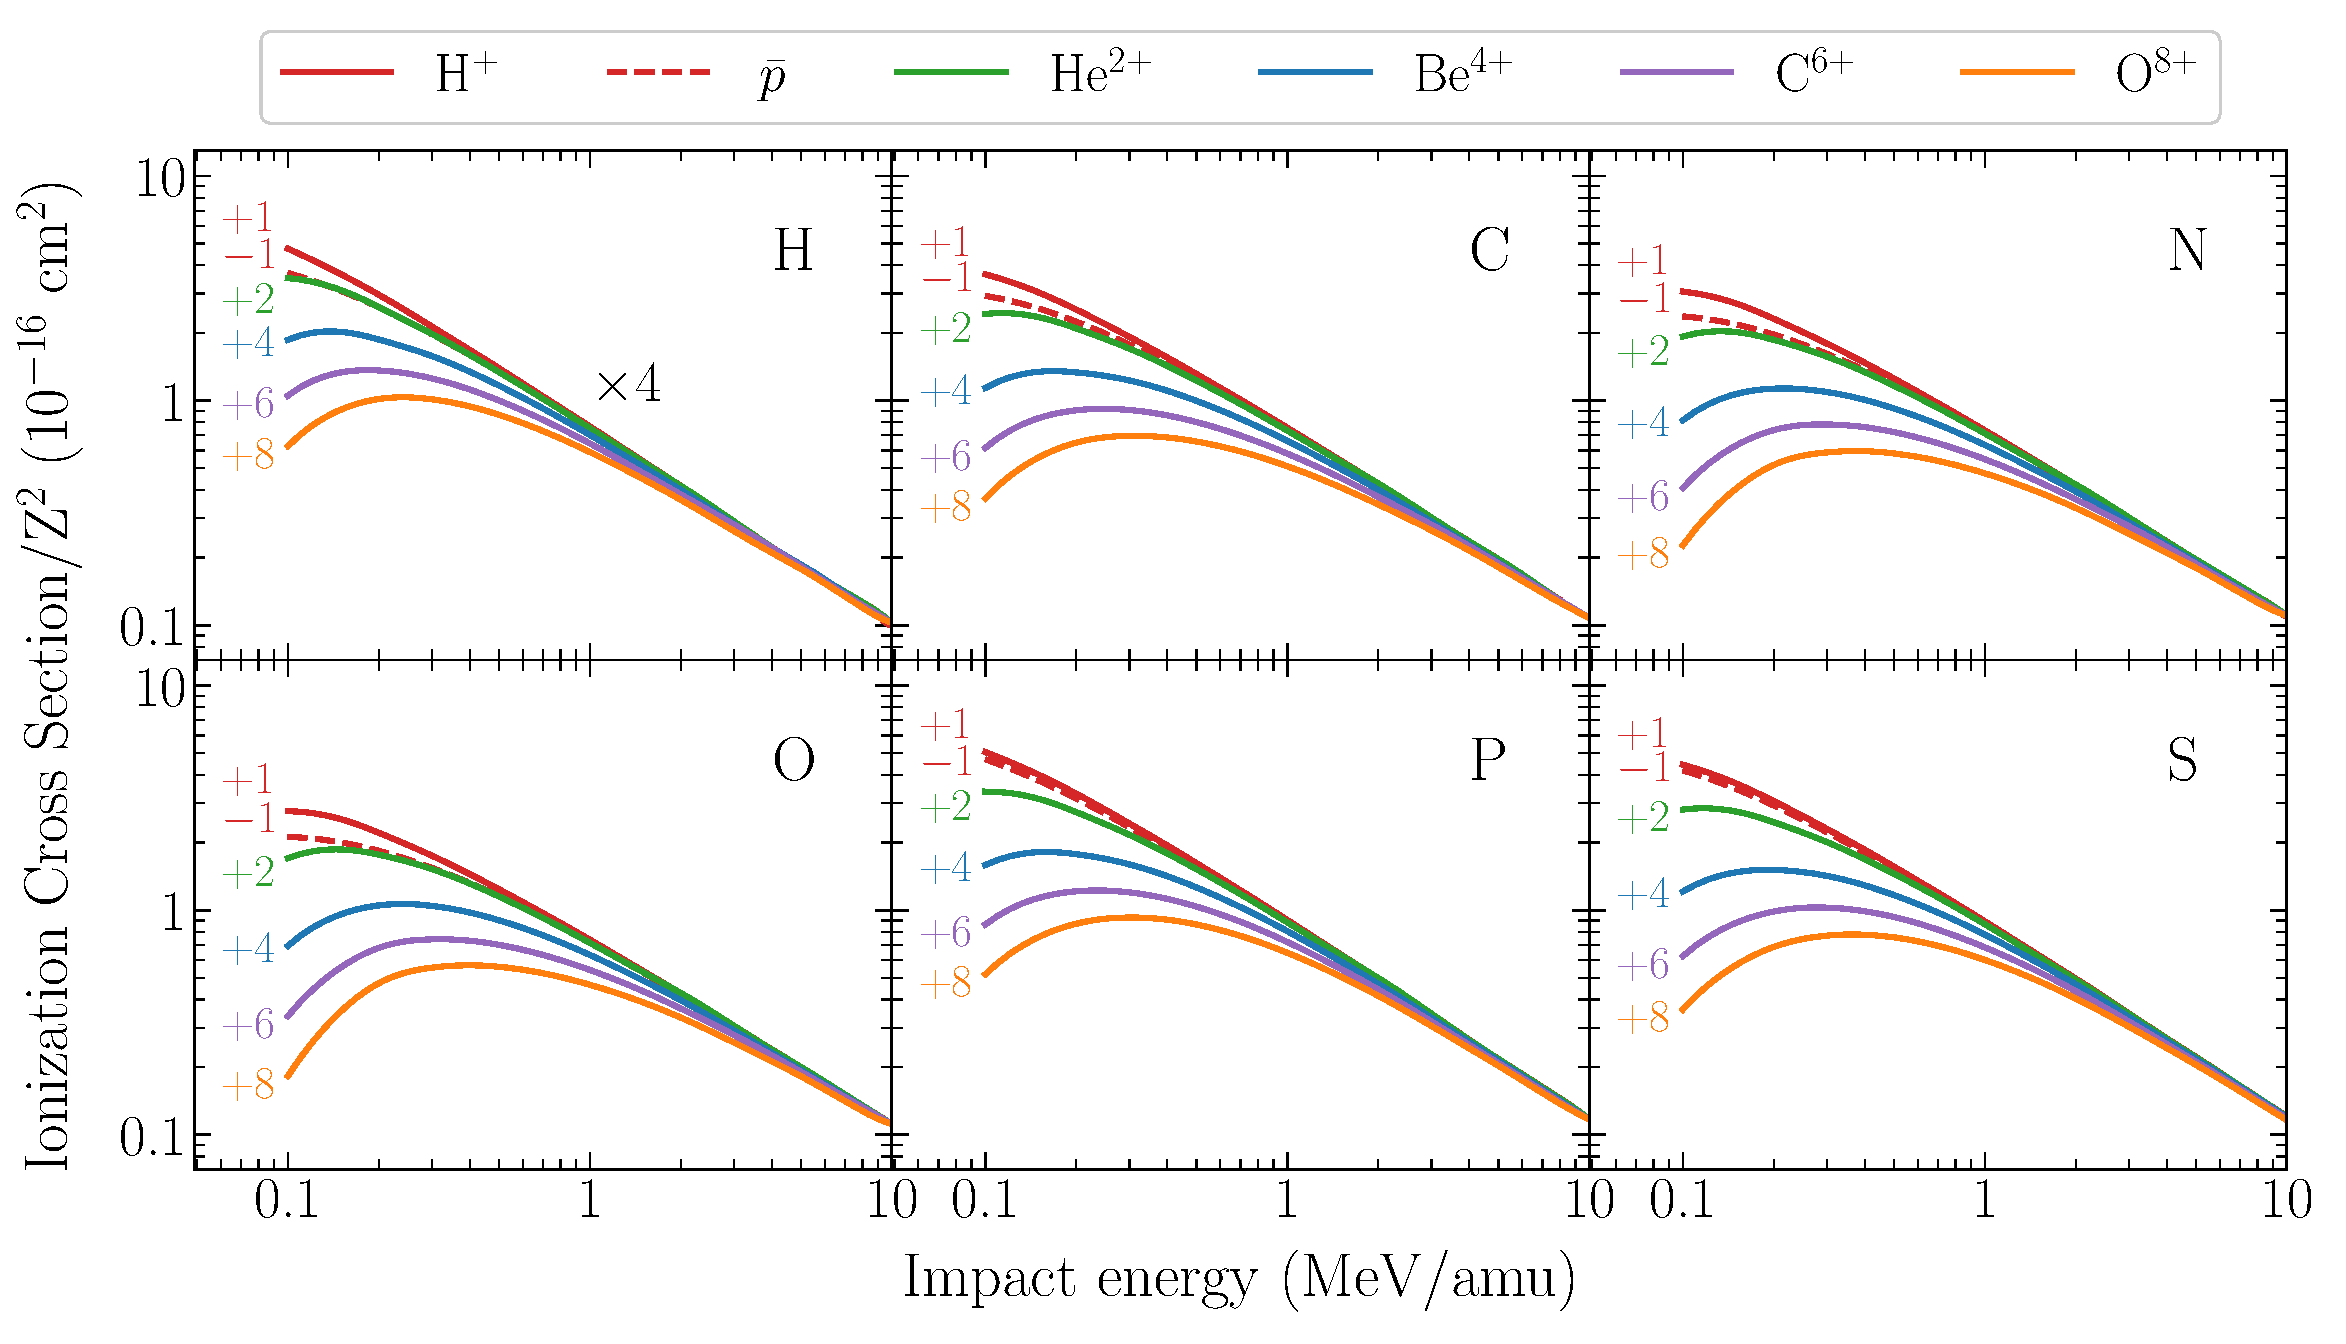
\includegraphics[width=0.9\textwidth]{ionmol/atomicscaling.eps}
\caption[Sección eficaz total de ionización atómica CDW reducida.]
{Sección eficaz total de ionización CDW reducida $\sigma_{\alpha}/Z^2$ 
de cuatro blancos atómicos relevantes. Curvas: cálculos teóricos CDW. 
Símbolos: ionización de H por impacto de H$^+$~\cite{Shah:81}; ionización 
por impacto de $e^-$ en H~\cite{Shah:87}, C~\cite{Brook:78}, 
N~\cite{Brook:78} y O~\cite{Thompson:95}.}
\label{fig:atomscaling}
\end{figure} 

La mayor parte de las moléculas orgánicas contienen átomos de hidrógeno, 
carbono, nitrógeno, oxígeno, fósforo y azufre. Los sistemas colisionales
que estudiamos a continuación están compuestos por cuatro blancos 
atómicos, $\alpha=$ H, C, N, O, y sies proyectiles incidentes: 
antiprotones $\bar{p}$, H$^{+}$, He$^{2+}$, Be$^{4+}$, C$^{6+}$, y 
O$^{8+}$. En la Fig.~\ref{fig:atomscaling} se muestran las secciones 
eficaces totales de ionización de los 24 sistemas blanco--proyectil 
resultantes usando el método CDW. Para comparar los resultados 
correspondiente a cada sistema colisional en una única figura, 
consideramos el hecho que en la primera aproximación de Born, la sección 
eficaz de ionización escala con el cuadrado de la carga del ion 
incidente, es decir $Z^{2}$. Las energías de impacto consideradas van de 
$0.1$ a 10 MeV/amu, donde el método CDW tiene validez. Particularmente, 
para los proyectiles de carga más altas, el valor de energía mínimo donde 
se espera que la CDW tenga validez aumenta hasta aproximadamente 400~keV. 
Nuestros resultados se comparan con secciones eficaces experimentales 
para el caso de ionización de H por impacto de H$^+$~\cite{Shah:81}. Se 
incluyen mediciones de ionización por impacto de electrones en 
H~\cite{Shah:87}, C~\cite{Brook:78}, N~\cite{Brook:78} y 
O~\cite{Thompson:95}, con la correspondiente conversión de equivelocidad, 
para energías incidentes superiores a 300~eV. Es esperable que en esta 
región de energía la ionización por impacto de H$^+$ y $e^-$ convergen. 
También realizamos cálculos similares con la FBA (no se muestran aquí), 
y corroboramos que ésta provee resultados confiables para valores de 
energía mayores a unos cuantos MeV/amu. Para nuestros resultados teóricos,
usamos el mismo color de línea para indicar la carga del proyectil en 
todas las figuras que se muestran a lo largo de este Capítulo: 
discontinua--roja, sólida--roja, azul, magenta, oliva y naranja para 
antiprotones, H$^{+}$, He$^{2+}$, Be$^{4+}$, C$^{6+}$, y O$^{8+}$, 
respectivamente. En el caso de los datos experimentales, se usan símbolos 
de los mismos colores para denotar la carga del ion incidente 
correspondiente. Los resultados de ionización de cada capa se pueden 
hallar en la Ref.~\cite{Miraglia:19}.

%%%%%%%%%%%%%%%%%%%%%%%%%%%%%%%%%%%%%%%%%%%%%%%%%%%%%%%%%%%%%%%%%%%%%%%%
\subsection{Distribución energética de electrones}
\label{subsec:meanener}
%%%%%%%%%%%%%%%%%%%%%%%%%%%%%%%%%%%%%%%%%%%%%%%%%%%%%%%%%%%%%%%%%%%%%%%%

En un medio biológico dado, la ionización directa debido al impacto de un 
ion representa solo una fracción del daño total. Los electrones 
secundarios, así como el retroceso de los iones del blanco, también 
contribuyen sustancialmente al daño total~\cite{Denifl:11}. Podemos 
considerar que la sección eficaz de ionización diferencial en función de 
la energía del electrón eyectado $E$ de la capa $nl$ del átomo $\alpha$,
$d\sigma_{\alpha nl}/dE$, es una función de distribución simple~\cite{Surdutovic:18}. Así, siguiente a Abril y 
coloboradores~\cite{Abril:15}, definimos un valor medio 
$\overline{E}_{\alpha}$, 
\begin{eqnarray}
\overline{E}_{\alpha} &=&\frac{\langle E_{\alpha}\rangle}{\langle
1\rangle}=\frac{1}{\sigma_{\alpha}}\sum\limits_{nl}\int dE\,E
\frac{d\sigma_{\alpha,nl}}{dE}\,,  
\label{eq:meanener} \\
\langle 1\rangle &=&\sigma_{\alpha}=\sum\limits_{nl}\int dE\,
\frac{d\sigma_{\alpha,nl}}{dE}\,. 
\label{eq:normener}
\end{eqnarray}
donde $\Sigma_{nl}$ tiene en cuenta la suma de las diferentes 
contribuciones de cada capa del elemento $\alpha$.

\begin{figure}
\centering
\includegraphics[width=0.9\textwidth]{ionmol/ener_mean.eps}
\caption[Distribución energética media de electrones emitidos.]
{Distribución energética media de electrones emitidos por la ionización 
debido al impacto de iones cargados dada por la Ec.~(\ref{eq:meanener}). 
Curvas: cálculos teóricos FBA con $Z=1$ (punteada) y CDW (sólidas y 
discontinua).}
\label{fig:emittedener}
\end{figure} 

Las energías medias de los electrones emitidos $\overline{E}_{\alpha}$ 
por H, C, N y O se muestran en la Fig.~\ref{fig:emittedener}. El rango 
de velocidad de impacto fue reducido a $v=10$~a.u. debido a las 
limitaciones numéricas en la expansión de esféricos armónicos dados por 
la Ec.~(\ref{eq:contwave}). A medida que la velocidad de impacto $v$ 
aumenta, también aumenta $\langle E_{\alpha}\rangle$ y $l_{\max}$, lo que 
resulta en la inclusión de funciones con muchas oscilaciones en el 
integrando. Más aún, el integrando de $\langle E_{\alpha}\rangle$ incluye 
la energía cinética $E$, que reduce su valor en la región de energías 
pequeñas y lo incrementa para valores grandes, haciendo que el resultado 
sea más sensible a los momentos angulares mayores. Independientemente, 
para $v>10$ a.u., la primera aproximación de Born es válida. 

En la Fig.~\ref{fig:emittedener} estimamos el valor de 
$\overline{E}_{\alpha}$ de los electrones emitidos en el rango de energía 
de 10 a 70 eV, para todos los blancos atómicos. Nuestros resultados 
concuerdan con los hallazgos experimentales~\cite{Surdutovic:18}. Como se 
puede observar en la figura, el valor de energía media es 
sorprendentemente sensible a la carga del proyectil $Z$, que puede 
duplicar los resultados de protón en la región intermedia, i.e., 
100--400 keV/amu. El efecto observado puede atribuirse al repulsión 
electrónica causada por los iones de carga múltiple en los electrones de 
baja energía. Este comportamiento no se puede encontrar en la primera 
aproximación de Born, donde la ley de escala $Z^2$ cancela la dependencia 
con $Z$ de la Ec.~(\ref{eq:meanener}). A altas energías, 
$\overline{E}_{\alpha}$ tiende a un valor universal para todos los iones, 
como puede verse en la Fig.~\ref{fig:emittedener}.

%%%%%%%%%%%%%%%%%%%%%%%%%%%%%%%%%%%%%%%%%%%%%%%%%%%%%%%%%%%%%%%%%%%%%%%%
\subsection{Distribución angular de electrones}
\label{subsec:meanang}
%%%%%%%%%%%%%%%%%%%%%%%%%%%%%%%%%%%%%%%%%%%%%%%%%%%%%%%%%%%%%%%%%%%%%%%%

\begin{figure}
\centering
\includegraphics[width=0.9\textwidth]{ionmol/ang_mean.eps}
\caption[Distribución angular media de electrones emitidos.]
{Distribución angular media de electrones emitidos por la ionización 
debido al impacto de iones cargados dada por Ec.~(\ref{eq:meanang}). 
Curvas: cálculos teóricos FBA con $Z=1$ (punteada) y CDW (sólidas y 
discontinua).}
\label{fig:emittedang}
\end{figure} 

Como mencionamos anteriormente, la emisión de electrones secundarios 
contribuye al daño total. Entonces, no sólo es esencial conocer la 
distribución de energía de los electrones eyectados, sino también la 
dirección a la que éstos son emitidos. Una vez más, podemos considerar 
que la sección eficaz diferencial de ionización es función del ángulo 
sólido de eyección del electrón $\Omega$, $d\sigma_{\alpha,nl}/d\Omega$, 
y puede expresarse como una función de distribución. Así, el ángulo medio 
de emisión $\overline{\theta}_{\alpha}$ se define como
\begin{eqnarray}
\overline{\theta}_{\alpha}&=&\frac{\langle\theta_{\alpha}\rangle}
{\langle 1\rangle}=\frac{1}{\sigma_{\alpha}}\sum\limits_{nl}
\int d\Omega\,\theta\,\frac{d\sigma_{\alpha,nl}}{d\Omega} 
\label{eq:meanang} \\
\langle 1\rangle &=&\sigma_{\alpha}=\sum\limits_{nl}\int d\Omega\,
\frac{d\sigma_{\alpha,nl}}{d\Omega}\,.
\end{eqnarray}

Los ángulos medios de emisión electrónica $\overline{\theta}_{\alpha}$ 
de los cuatro átomos y seis iones estudiados en esta sección se muestran 
en la Fig.~\ref{fig:emittedang}. Se puede observar una dependencia 
significativa de $\overline{\theta}_{\alpha}$ con $Z$ para todos los 
sistemas colisionales. Una vez más, este efecto no puede ser observado en 
la implementación del FBA (línea punteada).

En la emisión de electrones de baja energía, la dispersión angular es 
casi isotrópica~\cite{Rudd:92}. Un valor típico para el ángulo de 
eyección considerado en la literatura es 
$\overline{\theta}_{\alpha}\sim$~70\textdegree~\cite{Surdutovic:18}, el 
cual resulta bastante certero en el rango de validez de la FBA para 
cualquier blanco. Sin embargo, cuando se usa la aproximación de onda 
distorsionada, $\overline{\theta}_{\alpha}$ disminuye sustancialmente con 
$Z$ en la región de energía intermedia, como se observa en la 
Fig.~\ref{fig:emittedang}. Cuanto mayor sea la carga $Z$, menor será 
$\overline{\theta}$. Por supuesto, este efecto solo es válido en energías 
intermedias y no en el rango de altas energías.

Para ilustrar esta característica, consideramos el impacto de C$^{6+}$ 
con una energía de 500~keV sobre oxígeno. La primera aproximación de Born 
predice electrones emitidos con energías medias de $46.7$ eV y ángulos 
medios de 78\textdegree, mientras que la aproximación CDW establece 
energías medias de $62.5$~eV y un ángulo de emisión igual a 60\textdegree. 
Nuestros resultados sugieren una penetración más profunda de los 
electrones secundarios con una orientación más cercana a la dirección del 
ion. Podemos atribuir esta corrección de la dirección de avance al efecto 
de captura del continuo.

Además, la Fig.~\ref{fig:emittedang} proporciona una descripción 
ilustrativa del comportamiento de los antiprotones: el proyectil repele 
los electrones, siendo $\overline{\theta}_{\alpha}\sim$~90\textdegree. 
Nótese el descripción opuesta de protones y antiprotones dada por la CDW 
con respecto a la primera aproximación de Born; este fenómeno constituye 
un efecto Barkas angular.

%%%%%%%%%%%%%%%%%%%%%%%%%%%%%%%%%%%%%%%%%%%%%%%%%%%%%%%%%%%%%%%%%%%%%%%%
\section{El modelo estequiométrico}
\label{sec:SSM}
%%%%%%%%%%%%%%%%%%%%%%%%%%%%%%%%%%%%%%%%%%%%%%%%%%%%%%%%%%%%%%%%%%%%%%%%

El modelo estequiométrico simple (\acs{ssm}) que proponemos aquí para 
predecir secciones eficaces moleculares totales de ionización está basado 
en la aproximación de átomo independiente, también llamada regla aditiva 
de Bragg. Este modelo supone que los átomos que componen una molécula $M$ 
interactúan con el proyectil incidente pero no entre sí. Así, si 
suponemos que la molécula $M$ está compuesta por $n_{\alpha}$ átomos del 
elemento $\alpha$, el modelo estequiométrico aproxima la sección eficaz 
total de ionización de la molécula $\sigma_M$ como la suma de secciones 
eficaces totales de ionización de los átomos aislados $\sigma_{\alpha}$ 
ponderada por $n_{\alpha}$, 
\begin{equation}
\sigma_{M}=\sum\limits_{\alpha}n_{\alpha}\sigma_{\alpha}\,.  
\label{eq:sumion}
\end{equation}
Los blancos moleculares examinados a lo largo de este capítulo se 
clasifican en tres familias: CH, CHNO, y ADN, como se muestra en la 
Tabla~\ref{tab:families}.

\begin{table}
\begin{center}
\begin{tabular}{|p{0.08\textwidth}|p{0.8\textwidth}|}
\hline
\multirow{2}{*}{CH} & CH$_4$ (metano), C$_2$H$_2$ (acetileno), 
C$_2$H$_4$ (eteno), C$_2$H$_6$ (etano), \\ & C$_6$H$_6$ (benceno) \\
\hline
\multirow{2}{*}{CHNO} & C$_5$H$_5$N (piridina), C$_4$H$_4$N$_2$ (pirimidina), 
C$_2$H$_7$N (dimetilamina), \\ & CH$_5$N (monometilamina), 
C$_4$H$_8$O (THF) \\[0.2em]
\hline
\multirow{2}{*}{DNA} & C$_5$H$_5$N$_5$ (adenina), C$_4$H$_5$N$_3$O (citosina), 
C$_5$H$_5$N$_5$O (guanina), \\ & C$_5$H$_6$N$_2$O$_2$ (timina),
C$_4$H$_4$N$_2$O$_2$ (uracilo), H$_2$O (agua) \\
\hline
\end{tabular}
\caption[Blancos moleculares examinados y clasificados en tres familias.]
{Blancos moleculares de interés examinados en el presente trabajo y 
clasificados en tres familias.}
\label{tab:families}
\end{center}
\end{table}

En la Fig.~\ref{fig:crossDNA_1} reportamos las secciones eficaces de 
ionización totales reducidas con la carga del ión incidente, 
$\sigma_M/Z^2$, de las nucleobases del ADN --adenina, citosina, guanina y 
timina-- debido al impacto de iones de carga múltiple, que se obtienen a 
partir de la aproximación SSM y el método CDW. Para adenina, los datos 
experimentales disponibles para el impacto de protones~\cite{Iriki:11} 
tienen un excelente acuerdo con nuestras 
predicciones. La medición de C$^{4+}$~\cite{Sens:20} sobre adenina 
coincide con el modelo SSM--CDW dentro del margen de error. Si bien esta
data es preliminar, la comparación es alentadora en cuanto a la respuesta 
de nuestro modelo para la ionización de projectiles de carga múltiple. 
Por otro lado, los resultados teóricos de ionización de adenina debido a 
C$^{6+}$ discrepan con el valor experimental 
disponible~\cite{Bhattacharjee:19} en un factor dos. Esta discrepancia es 
intrigante ya que la medición se encuentra en el rango de altas energías, 
donde generalmente la teoría predice muy bien los experimentos.

No hemos encontrado en la bibliografía datos experimentales de ionización 
por impacto de iones cargados para el resto de las nucleobases de ADN.
Incluimos en la Fig.~\ref{fig:crossDNA_1} mediciones de ionización por 
impacto de electrones~\cite{Rahman:16}, con la correspondiente 
conversión de equivelocidad, para energías incidentes superiores a 
300~eV. En esta región, la sección eficaz de ionización por impacto de 
protones y electrones debería coincidir. Aunque las mediciones de impacto 
de electrones están por encima de nuestros hallazgos para todos los 
objetivos moleculares, vale la pena señalar que los resultados SSM--CDW
concuerdan muy bien con otras predicciones teóricas de ionización por 
impacto de electrones~\cite{mozejko2003,tan2018}.

\begin{figure}
\centering
\includegraphics[width=0.9\textwidth]{ionmol/adn1.eps}
\caption[Sección eficaz total de ionización reducida por $Z$ (Parte I).]
{Sección eficaz total de ionización CDW reducida $\sigma_{M}/Z^2$ como 
una función de la energía de impacto del ion. Símbolos: datos 
experimentales de impacto de protón~\cite{Iriki:11}, 
C$^{4+}$~\cite{Sens:20}, C$^{6+}$~\cite{Bhattacharjee:19}, y 
e$^-$~\cite{Rahman:16} con conversión de equivelocidad.}
\label{fig:crossDNA_1}
\end{figure} 

\begin{figure}
\centering
\includegraphics[width=0.9\textwidth]{ionmol/adn2.eps}
\caption[Sección eficaz total de ionización reducida por $Z$ (Parte II).]
{Sección eficaz total de ionización CDW reducida $\sigma_{M}/Z^2$ como 
una función de la energía de impacto del ion. Símbolos: datos 
experimentales de impacto de protón en uracilo~\cite{itoh2013}, 
pirimidina~\cite{wolff2014}, THF~\cite{wang2016} y agua~\cite{Luna2007,
Bolorizadeh86,H_Rudd85,toburen80}. Impacto de C$^{4+}$~\cite{Sens:20} y 
C$^{4+}$, C$^{6+}$, O$^{6+}$, F$^{6+}$, O$^{8+}$, y F$^{8+}$ en 
uracilo~\cite{agnihotri2012,agnihotri2013}. Ionización de agua por 
impacto de He$^{2+}$~\cite{Ohsawa05,He_Rudd85,toburen80}, 
C$^{6+}$~\cite{DalCappello2009,Bhattacharjee:17} y 
O$^{8+}$~\cite{Bhattacharjee:16}. 
Impacto de e$^-$~\cite{bug2017,wolf2019,fuss2009} con conversión de 
equivelocidad.}
\label{fig:crossDNA_2}
\end{figure} 

Las secciones eficaces de ionización total reducidas $\sigma_M/Z^2$ 
para uracilo, pirimidina, THF y agua se muestran en la 
Fig.~\ref{fig:crossDNA_2}. En uracilo, las mediciones experimentales de 
ionización por impacto de protones de Itoh~\textit{et al.}~\cite{itoh2013} 
tienen un buen acuerdo con nuestras predicciones. Sin embargo, para el 
mismo blanco, nuestra teoría predice secciones eficaces con un factor 
dos por encima de las mediciones experimentales de Agnihotri 
\textit{et al.}~\cite{agnihotri2012,agnihotri2013} para el impacto de 
iones de carga múltiple. No obstante, cabe señalar que nuestros 
resultados teóricos coinciden con los cálculos de Champion, Rivarola y 
colaboradores~\cite{agnihotri2012,champion2012}. Los cálculos recientes 
de Sarkadi~\cite{sarkadi2016} empleando el método CTMC también se 
encuentran por arriba de los valores experimentales de Tribedi y 
colaboradores~\cite{agnihotri2012,agnihotri2013}. Además, hemos incluimos 
una reciente medición experimental preliminar de Sens y 
colaboradores~\cite{Sens:20} para la ionización en uracilo debido al 
impacto de C$^{4+}$ que coincide con la teoría, lo que podría indicar 
algún problema con los valores experimentales de Agnihotri y 
colaboradores. 

Para pirimidina, mostramos una comparación de nuestros resultados con los 
datos experimentales de ionización por impacto de protones de Wolff
\textit{et al.}~\cite{wolff2014} y también para la ionización por impacto 
de electrones~\cite{bug2017} a altas energías. Las mediciones de impacto 
de electrones concuerdan con las predicciones SSM--CDW para energías 
superiores a 500~keV. Inesperadamente, las secciones eficaces de 
ionización por impacto de protones son significativamente más bajas que 
nuestros resultados. Una mayor cantidad de experimentos se encuentran 
disponibles para la ionización de la molécula de THF por impacto de 
H$^+$~\cite{wang2016} y de e$^-$~\cite{bug2017,wolf2019,fuss2009}. Los 
resultados que obtenemos de la combinación del SSM y las secciones 
eficaces atómicas CDW muestran un buen acuerdo general con esta data.

En el caso de la molécula de agua, los resultados experimentales son más 
abundantes que para el resto de los blancos. Los resultados 
experimentales~\cite{Luna2007,Bolorizadeh86,H_Rudd85,Ohsawa05,He_Rudd85,
toburen80,Bhattacharjee:16} coinciden con nuestras predicciones para 
todos los iones de carga múltiple examinados aquí, excepto para 
C$^{6+}$~\cite{DalCappello:09,Bhattacharjee:17}, donde la teoría 
sobrestima la ionización en un factor dos en el rango de altas energías. 
A diferencia de las nucleobases, pirimidina y THF, la estequiometría del 
agua es más simple; sin embargo, observamos que nuestro modelo responde 
bien incluso para predecir la ionización de moléculas pequeñas debido a 
la incidencia de iones pesados, tal como es el caso de O$^{6+}$.

%%%%%%%%%%%%%%%%%%%%%%%%%%%%%%%%%%%%%%%%%%%%%%%%%%%%%%%%%%%%%%%%%%%%%%%%
\section{Reglas de escala}
\label{sec:scaling}

%%%%%%%%%%%%%%%%%%%%%%%%%%%%%%%%%%%%%%%%%%%%%%%%%%%%%%%%%%%%%%%%%%%%%%%%
\subsection{Escala con electrones activos del blanco}
\label{subsec:ne_scaling}

%%%%%%%%%%%%%%%%%%%%%%%%%%%%%%%%%%%%%%%%%%%%%%%%%%%%%%%%%%%%%%%%%%%%%%%%
\subsubsection{Regla de Toburen}
\label{subsec:toburen}
%%%%%%%%%%%%%%%%%%%%%%%%%%%%%%%%%%%%%%%%%%%%%%%%%%%%%%%%%%%%%%%%%%%%%%%%

Toburen y colaboradores~\cite{Toburen:75,Toburen:76} propusieron el 
primer modelo fenomenológico completo y simple para la eyección de 
electrones de moléculas complejas. Los autores encontraron conveniente 
escalar la sección eficaz de ionización experimental en términos del 
número de electrones ligados débilmente, o activos, $n_e$. En general, 
este número está dado por la cantidad de electrones en la capa de 
valencia. Así, por ejemplo, para C, N y O, este número es igual al número 
total de electrones del átomo menos la capa K. 

Siguiendo a Toburen \textit{et al.}, definimos la sección eficaz de 
ionización escalada por el número de electrones débilmente ligado 
$\sigma_e$ para la molécula $M$ como
\begin{equation}
\sigma_e=\frac{\sigma_M}{n_e}\,, 
\label{eq:cross-ne} 
\end{equation}
donde $n_e=\sum_{\alpha}n_{\alpha}\nu_{\alpha}$ es el número total de 
electrones activos en el proceso colisional, y $\nu_{\alpha}$ es el 
número de electrones débilmente ligado en cada átomo $\alpha$. Para los 
blancos atómicos considerados aquí, los números de Toburen están dados 
por 
\begin{equation}
\nu_{\alpha}^T=\left\{ 
\begin{array}{ll}
1, & \text{para H,} \\
4, & \text{para C,} \\ 
5, & \text{para N,} \\ 
6, & \text{para O}\,.
\end{array}\right.
\label{eq:neToburen} 
\end{equation} 

La regla de Toburen se puede enunciar diciendo que $\sigma_{e}$ es un 
parámetro universal, que depende únicamente de la velocidad y naturaleza
del ion incidinte, aplicable en la región de $0.25$ a 5~MeV/amu. A 
muy altas energías, la probabilidad de ionizar electrones de la capa K 
es mayor. Así, en esta región, el número total de electrones activos 
será diferente. Una dependencia similar con el número de electrones 
ligados débilmente fue hallada por Itoh y coloboradores~\cite{itoh2013} 
para el impacto de protones sobre uracilo y adenina.

Siguiendo la ley de escala de Toburen, calculamos las secciones eficaces 
CDW escaladas con el número de electrones activos de Toburen, 
$\sigma_{e}^T$, para los blancos moleculares dados en la 
Tabla~\ref{tab:families}. Nuestros resultados se muestran en la 
Fig.~\ref{fig:newscaling}(a) en función de la energía de impacto para 
diferentes proyectiles de carga múltiple. Aunque la escala de Toburen se 
mantiene para altas energías, su desempeño no es muy satisfactorio: como 
se puede observar en la figura, la banda universal es bastante ancha.

\begin{figure}[t]
\centering
\includegraphics[width=0.9\textwidth]{ionmol/CDWscaling.eps}
\caption[Sección eficaz de ionización molecular escalada por $n_e$.]
{Sección eficaz de ionización molecular escalada por número de electrones 
débilmente ligados usando (a)~los números de Toburen $\nu_{\alpha}^T$, y 
(b) los números CDW $\nu_{\alpha}^{\text{CDW}}$ propuestos para las 
moléculas enlistadas en la tabla~\ref{tab:families}. Símbolos: 
datos experimentales de las Figs.~\ref{fig:crossDNA_1} y 
\ref{fig:crossDNA_2}.}
\label{fig:newscaling}
\end{figure}

%%%%%%%%%%%%%%%%%%%%%%%%%%%%%%%%%%%%%%%%%%%%%%%%%%%%%%%%%%%%%%%%%%%%%%%%
\subsubsection{Números CDW}
\label{subsec:CDW}
%%%%%%%%%%%%%%%%%%%%%%%%%%%%%%%%%%%%%%%%%%%%%%%%%%%%%%%%%%%%%%%%%%%%%%%%

La respuesta de nuestros resultados teóricos a la regla de escala de 
Toburen se puede entender inspeccionando la Fig.~\ref{fig:neCDW}. La 
figura muestra las secciones eficaces de ionización CDW de los átomos H, 
C, N y O debido al impacto de H$^+$ escaladas por el número de electrones 
activos de cada átomo. La Fig.~\ref{fig:neCDW}(a) muestra los resultados
CDW escalados con los números de Toburen dados por la 
Ec.~\ref{eq:neToburen}. La regla de Toburen no es satisfecha de manera 
apropiada por los cálculos CDW: para un valor de energía dado, los 
valores teóricos de ionización CDW escalados 
$\sigma_{\alpha}/\nu_{\alpha}^T$ de cada blanco atómico no son 
constantes. Por otro lado, si observamos los valores teóricos de 
ionización de O dados en la Fig.~\ref{fig:atomscaling}, notamos que éstos 
son muy similares a las secciones eficaces de C; esto pareciera sugerir 
que elnúmero de electrones activos en el átomo de O es cuatro en lugar de 
seis. De la misma manera, el número de electrones activos para N, que se 
obtienen a partir de los resultados teóricos CDW, también son diferentes 
de los dados por la Ec.~(\ref{eq:neToburen}). La Fig.~\ref{fig:neCDW}(b) 
muestra la respuesta de nuestros cálculos teóricos atómicos a estos 
nuevos valores.

\begin{figure}[t]
\centering
\includegraphics[width=0.9\textwidth]{ionmol/neCDW.eps}
\caption[Sección eficaz de ionización atómica escalada por $n_e$.]
{Sección eficaz de ionización atómica por impacto de H$^+$ escalada por 
electrón débilmente ligado usando (a)~los números de Toburen 
$\nu_{\alpha}^T$, y (b) los números CDW $\nu_{\alpha}^{\text{CDW}}$ }
\label{fig:neCDW}
\end{figure}

A partir del estudio sistemático de nuestros resultados teóricos de 
ionización en átomos, proponemos una optimización a la regla de Toburen. 
Así, el número total de electrones activos de la molécula $M$ en la 
Ec.~(\ref{eq:cross-ne}) está ahora dado por 
\begin{equation}
n_e'=\sum_{\alpha}n_{\alpha}\nu_{\alpha}^{\text{CDW}}\,,
\end{equation}
donde $\nu_{\alpha}^{\text{CDW}}$ son los números de electrones activos 
por átomo, que han sido optimizados a partir de las secciones eficaces 
de ionización CDW atómicas. Los números CDW están dados por
\begin{equation}
\nu_{\alpha }^{\text{CDW}} \sim\left\{ 
\begin{array}{ll}
1, & \text{para H,} \\
4, & \text{para C, N, y O}\,. \\ 
%4.5, & \text{para P y S}\,.
\end{array}
\right. 
\label{eq:neCDW}
\end{equation}

A partir de la Ec.~(\ref{eq:neCDW}), definimos nuevos números de 
electrones activos $n_e'$ para las moléculas consideradas hasta ahora.  
En la Tabla~\ref{tab:ne_molecules} mostramos algunos valores optimizados 
$n_e'$ y los números de Toburen $n_e$. Nuestros resultados son diferentes  
a los propuestos por Toburen, los cuales son utilizados por otros 
autores~\cite{itoh2013}, principalmente debido a las diferencias en los 
números de electrones activos del oxígeno. Las secciones eficaces 
moleculares escaladas por $n_e'$ se muestran en la 
Fig.~\ref{fig:newscaling}(b). Los datos experimentales para la ionización 
de adenina~\cite{Iriki:11,Sens:20,Bhattacharjee:19}, 
uracilo~\cite{itoh2013,Sens:20}, pirimidina~\cite{wolff2014}, 
THF~\cite{wang2016} y agua~\cite{Luna2007,Bolorizadeh86,H_Rudd85,
toburen80,Ohsawa05,He_Rudd85,DalCappello:09,Bhattacharjee:17,
Bhattacharjee:16} por impacto de iones cargados que se muestran en la 
Fig.~\ref{fig:newscaling}(b) validan nuestra optimización a la regla de 
escala de Toburen. También incluimos mediciones de ionización por 
impacto de electrones con conversión de equivelocidad en 
pirimidina~\cite{bug2017} y THF~\cite{bug2017,wolf2019,fuss2009}. Será 
interesante verificar nuestras predicciones con experimentos futuros, 
principalmente para estados de carga de proyectiles más altos.

\begin{table}
\begin{center}
\begin{tabular}{|p{0.12\textwidth}p{0.15\textwidth}p{0.03\textwidth}
p{0.03\textwidth}|p{0.12\textwidth}p{0.15\textwidth}p{0.03\textwidth}
p{0.03\textwidth}|}
\hline
Molécula        & Nombre      & $n_e$ & $n_e'$ & 
Molécula        & Nombre      & $n_e$ & $n_e'$ \\
\hline
H$_2$           & Dihidrógeno & 2      & 2     & 
C$_4$H$_4$N$_2$ & Pirimidina  & 30     & 28    \\
H$_2$O          & Agua        & 8      & 6     & 
C$_6$H$_6$      & Etano       & 30     & 30    \\
NH$_3$          & Amoníaco    & 8      & 7     & 
C$_4$H$_4$N$_2$O$_2$ & Uracilo & 40    & 36    \\
CH$_4$          & Metano      & 8      & 8     & 
C$_4$H$_5$N$_3$O & Citosina   & 42     & 37    \\
CH$_5$N         & Metilamina  & 14     & 13    & 
C$_5$H$_6$N$_2$O$_2$ & Timina & 48     & 42    \\
C$_2$H$_7$N     & Etilamina   & 20     & 19    & 
C$_5$H$_5$N$_5$ & Adenina     & 50     & 45    \\
C$_4$H$_8$O     & THF         & 30     & 28    & 
C$_5$H$_5$N$_5$O & Guanina    & 56     & 49    \\
\hline
\end{tabular}
\caption[Números de electrones activos moleculares de Toburen y CDW.]
{Número de electrones débilmente ligados según Toburen $n_e$ y 
optimización CDW~$n_e'$ para algunos blancos moleculares de interés 
biológico.}
\label{tab:ne_molecules}
\end{center}
\end{table}

\begin{figure}[t]
\centering
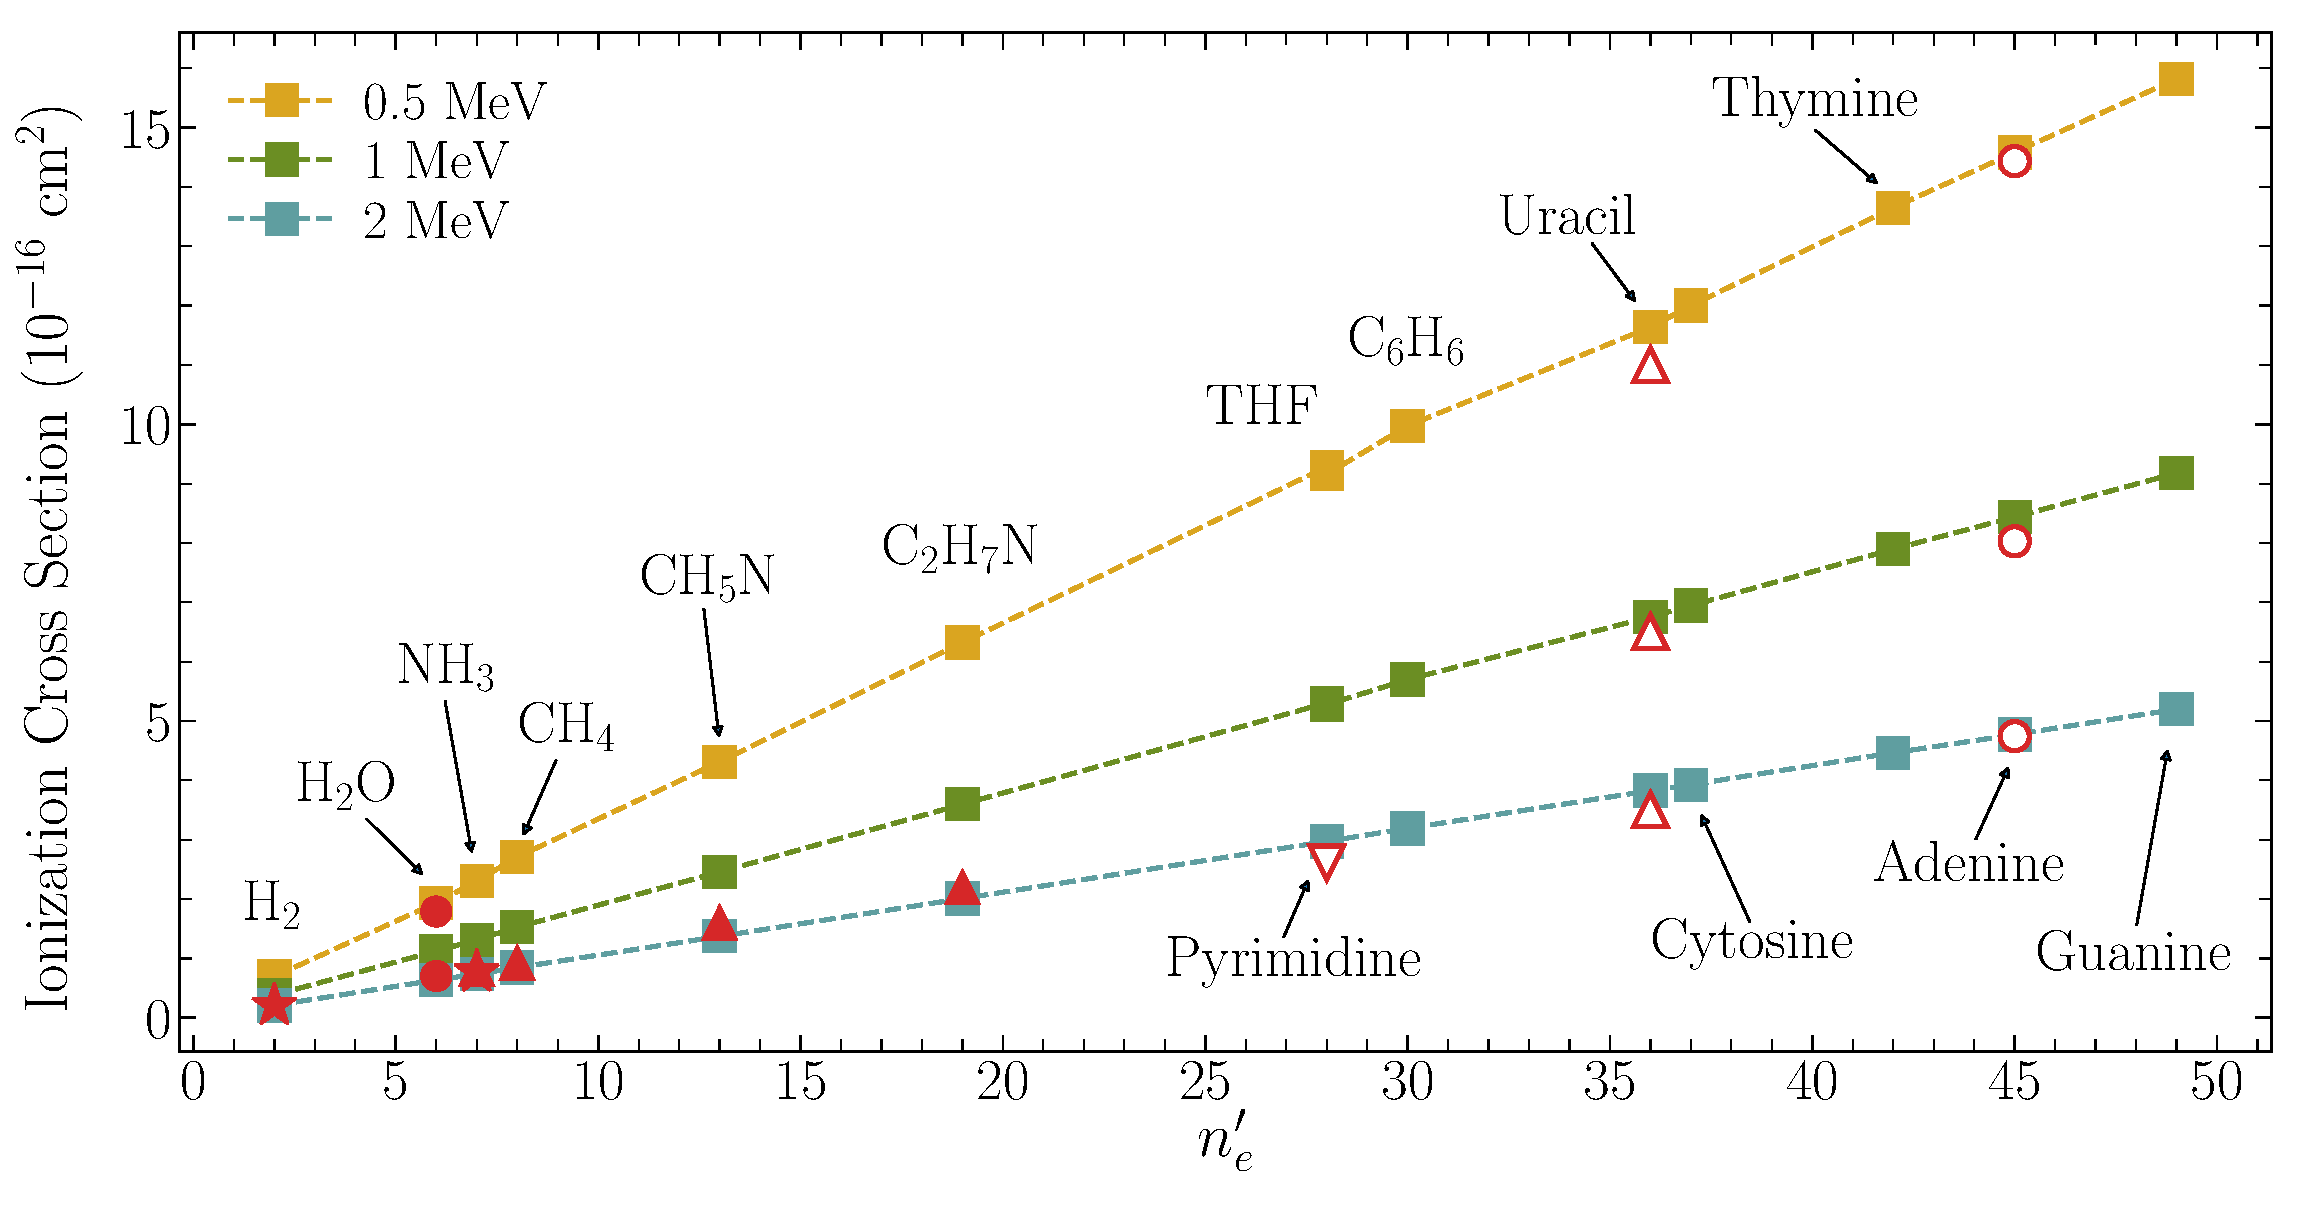
\includegraphics[width=0.9\textwidth]{ionmol/scale_ne.eps}
\caption[Ionización por impacto de protón en términos de $n_e'$.]
{Sección eficaz de ionización por impacto de protón a $0.5$, 1, y 2~MeV 
en términos del númbero de electrones activos dado por la 
Tabla~\ref{tab:ne_molecules}. Símbolos: 
\mbox{\Large$\circ$}~adenina~\cite{Iriki:11}, 
$\triangle$ uracilo~\cite{itoh2013}, 
$\bigtriangledown$ pirimidina~\cite{wolff2014}, 
$\blacktriangle$ C$_2$H$_7$N, CH$_5$N, metano y amoníaco~\cite{Lynch:76},
\mbox{\scriptsize$\bigstar$} amoníaco y H$_2$~\cite{Rudd:85}, y 
\mbox{\Large$\bullet$} agua~\cite{Luna2007}.}
\label{fig:recta}
\end{figure}

Podemos examinar de forma alternativa la escala definida por los números 
CDW dibujando las secciones eficaces de ionización de las moléculas en 
función de los valores dados para $n_e'$ según la 
Tabla~\ref{tab:ne_molecules} en ciertos valores de energía. Nuestros 
resultados se muestran en la Fig.~\ref{fig:recta} para energías de 
impacto de $0.5$, 1 y 2~MeV. Como puede observarse, las secciones 
eficaces de ionización CDW calculadas para todas las moléculas muestran 
una dependencia lineal con el número de electrones CDW $n_e'$ de la 
Tabla~\ref{tab:ne_molecules}. Obtenemos resultados similares, incluso 
para $E=10$~MeV. La comparación con los datos experimentales disponibles 
muestra una buena concordancia general, desde moléculas pequeñas, tales 
como H$_2$, CH$_4$ y NH$_3$, hasta las más complejas, como la adenina. 
Para los datos de ionización por impacto de electrón, los datos 
experimentales se interpolaron entre vecinos cercanos. 
%It is worth mentioning that an equivalent plot using the Toburen numbers 
%$n_e$ does not exhibit the straight lines obtained with the present scaling. 

%While finishing the present work, we became aware of an accepted 
%manuscript by L\"udde~\textit{et al.}~\cite{ludde2019} on total 
%ionization of biological molecules by proton impact, using the
%independent--atom--model pixel counting method~\cite{ludde2016,ludde2018}.
%The authors also raised a scaling  with $\nu_{\alpha}=4$ for C, N, and O. 
%The agreement with this independent method for proton impact reinforces 
%our multicharged--ion findings.

%%%%%%%%%%%%%%%%%%%%%%%%%%%%%%%%%%%%%%%%%%%%%%%%%%%%%%%%%%%%%%%%%%%%%%%%
\subsection{Escala con la carga del ion}
\label{sec:zscaling}
%%%%%%%%%%%%%%%%%%%%%%%%%%%%%%%%%%%%%%%%%%%%%%%%%%%%%%%%%%%%%%%%%%%%%%%%

A energías de impacto intermedias, la regla $Z^2$ no se cumple y se 
pueden considerar otras escalas en esta región. Encontramos en la 
literatura dos tipos de leyes de escala con la carga $Z$ del ion 
incidente aplicables en este rango de energías de impacto. La regla 
sugerida por Janev y Presnyakov~\cite{Janev:80} considera $\sigma/Z$ en 
función de $E/Z$ como la forma reducida \textit{natural} de la sección 
eficaz de ionización $\sigma$ y la energía de ion incidente $E$. Más 
recientemente, Montenegro y colaboradores~\cite{Dubois:13,Montenegro:13} 
sugirieron una expresión alternativa, la cual toma en cuenta que la 
sección eficaz es una función de $Z^2/E$ a altas energías. La escala 
propuesta, dada por
\begin{equation}
 \sigma/Z^{\alpha}=f(E/Z^{2-\alpha}),
\label{eq:Montenegro}
\end{equation}
mantiene la relación $Z^2/E$ para cualquier valor del parámetro $\alpha$. 
Los autores propusieron el valor $\alpha=4/3$ para la ionización de He y
H$_2$ debido al impacto de diversos iones cargados~\cite{Dubois:13}. 

Siguiendo el trabajo de Montenegro y colaboradores, optimizamos el 
parámetro~$\alpha$ de manera tal que los resultados obtenidos por la 
combinación del método CDW y SSM para los sistemas colisionales 
moleculares estudiados aquí convergan en el mayor rango de energías 
posible (de intermedias a altas). El resultado de dicha optimización es 
$\alpha=1.2$. La validez de este particular escaleo es evidente en la 
Fig.~\ref{fig:zreduced}, donde --para cada blanco-- las curvas SSM--CDW 
correspondientes a los diferentes iones se superponen. Es notable como 
los resultados teóricos son válidos para energías de impacto incluso por 
encima del máximo de las secciones eficaces, que corresponden a rangos de 
energías incidentes desde 50 keV para H$^+$ hasta 250 keV/amu para 
O$^{+8}$.

\begin{figure}
\centering
\includegraphics[width=0.9\textwidth]{ionmol/adn1_zscale.eps}
\caption[Sección eficaz de ionización reducida por $Z$ y $\alpha$ 
(Parte I).]
{Sección eficaz de ionización reducida $\sigma/Z^{\alpha}$ como función
de la energía incidente del ion $E/Z^{2-\alpha}$ con $\alpha=1.2$. 
Curvas: resultados teóricos CDW-SSM. 
Símbolos: datos experimentales de la Fig.~\ref{fig:crossDNA_1}.}
\label{fig:zreduced}
\end{figure} 

\begin{figure}
\centering
\includegraphics[width=0.9\textwidth]{ionmol/adn2_zscale.eps}
\caption[Sección eficaz de ionización reducida por $Z$ y $\alpha$ 
(Parte II).]
{Sección eficaz de ionización reducida $\sigma/Z^{\alpha}$ como función
de la energía incidente del ion $E/Z^{2-\alpha}$ con $\alpha=1.2$. 
Curvas: resultados teóricos CDW-SSM. 
Símbolos: datos experimentales de la Fig.~\ref{fig:crossDNA_2}.}
\label{fig:zreduced}
\end{figure} 

También examinamos los datos experimentales disponibles para los sistemas
ion-blanco bajo estudio~\cite{Iriki:11,Sens:20,Bhattacharjee:19,itoh2013,
wolff2014,wang2016,agnihotri2012,agnihotri2013,Luna2007,Bolorizadeh86,
H_Rudd85,He_Rudd85,toburen80,Ohsawa05,Bhattacharjee:17,DalCappello:09,
Bhattacharjee:16} con la regla de escala $Z^\alpha$. En el caso de los 
blancos con pocos o ningún dato experimental incluimos secciones eficaces 
experimentales de ionización por impacto de electrón~\cite{Rahman:16,
bug2017,wolf2019,fuss2009} a grandes velocidades con la conversión 
correspondiente. Como se observa, la mayor parte de los datos 
experimentales en la Fig.~\ref{fig:zreduced} confirma el escaleo sugerido 
aquí, incluso para O$^{+8}$ en agua~\cite{Bhattacharjee:16}. 

%%%%%%%%%%%%%%%%%%%%%%%%%%%%%%%%%%%%%%%%%%%%%%%%%%%%%%%%%%%%%%%%%%%%%%%%
\subsection{Escala con electrones activos y carga del ion}
\label{sec:nez_scaling}
%%%%%%%%%%%%%%%%%%%%%%%%%%%%%%%%%%%%%%%%%%%%%%%%%%%%%%%%%%%%%%%%%%%%%%%%

Considerando la reducción con la carga del ión incidente $Z^\alpha$ y el 
escaleo con el número de electrones activos del blanco, introducimos 
la sección eficaz de ionización molecular independiente $\tilde{\sigma}$, 
que se expresa como función de $\tilde{E}=E/Z^{2-\alpha}$, y está dada por
\begin{equation}
 \tilde{\sigma}\left(\tilde{E}\right)=\frac{\sigma_e}{Z^{\alpha}}
 =\frac{\sigma_M}{n_e'\,Z^{\alpha}}\,,
\label{eq:u-scaling}
\end{equation}
donde $\sigma_M$ es la sección eficaz de ionización de un blanco 
molecular, $n_e'$ es el número de electrones activos por molécula dado
en la Tabla~\ref{tab:ne_molecules}, y el parámetro es $\alpha=1.2$. La 
Fig.~\ref{fig:zalpha} muestra los valores teóricos y experimentales de 
$\tilde{\sigma}$ para todos los sistemas moleculares de la 
Tabla~\ref{tab:families}. Como se observa, la regla de escala combinada 
funciona muy bien y es independiente tanto de la naturaleza del ion 
incidente como de la complejidad del blanco molecular. Nuestros 
resultados teóricos SSM--CDW se ubican en una banda estrecha válida para 
cualquier ion incidente (reducida con $Z^\alpha$) en cualquier molécula
(escalada con el número de electrones activos $n_e'$) con una dispersión 
de aproximadamente $\pm 20\%$. Si consideramos los valores experimentales
disponibles, la incertidumbre de nuestra escala independiente crece a 
$\pm 30\%$, esquematizada en la Fig.~\ref{fig:zreduced} con un área gris. 
Notar que no hemos incluido en esta figura los resultados para uracilo de 
las Refs.~\cite{agnihotri2012,agnihotri2013}. 

\begin{figure}[t]
\centering
\includegraphics[width=0.9\textwidth]{ionmol/Zne_scaling.eps}
\caption[Sección eficaz de ionización reducida por $Z$ y $n_e$.]
{Sección eficaz de ionización reducida con la carga $Z$ del ion incidente
y escalada con el número de electrones activo $n_e$ del blanco molecular,
dado por la ecuación~(\ref{eq:u-scaling}) con $\alpha=1.2$. 
Curvas: resultados teóricos CDW-SSM. Símbolos: datos experimentales de 
las Figs.~\ref{fig:crossDNA_1} y \ref{fig:crossDNA_2}.}
\label{fig:zalpha}
\end{figure} 

Proponemos que la regla de escala independiente propuesta es válida para 
cualquier combinación ion--molécula. Para evaluar la generalidad de 
nuestro modelo, incluimos en la Fig.~\ref{fig:zreduced} un grupo de datos 
experimentales correspondientes a blancos moleculares no considerados en 
el diseño de esta regla, tales como las mediciones de 
Rudd~\textit{et al.}~\cite{Rudd:85,Rudd:83} para H$^{+}$ y He$^{+2}$ 
en N$_2$, O$_2$, CH$_4$, CO y CO$_2$, y los recientes experimentos de
Luna~\textit{et al.} \cite{Luna2019} de H$^{+}$ en CH$_4$. 

El buen acuerdo entre los resultados previstos por nuestro modelo y los
datos experimentales disponibles que se muestran en la 
Fig.~\ref{fig:zalpha} resume los principales resultados de esta 
investigación. Nuestro regla de escala independiente muestra ser eficaz 
no solo para predecir la ionización de los sistemas ion--blanco 
estudiados aquí sino también muestra potencial para reproducir una gran 
variedad de sistemas colisionales. Aunque los resultados teóricos 
SSM--CDW son válidos para energías por debajo del máximo de la sección 
eficaz de ionización, se puede observar en la Fig.~\ref{fig:zalpha} como 
el escaleo de los datos experimentales se extiene aún para valores de 
energía incidente menores. Esperamos que mediciones experimentales para 
otros iones y moléculas refuercen el modelo y escaleo propuesto.

%%%%%%%%%%%%%%%%%%%%%%%%%%%%%%%%%%%%%%%%%%%%%%%%%%%%%%%%%%%%%%%%%%%%%%%%
\section{Estructura molecular de los blancos}
\label{sec:molcalculations}
%%%%%%%%%%%%%%%%%%%%%%%%%%%%%%%%%%%%%%%%%%%%%%%%%%%%%%%%%%%%%%%%%%%%%%%%

Finalmente, para probar el rango de validez del SSM, realizamos un 
cálculo de estructura molecular de primeros principios para cinco 
nucleobases empleando el código {\sc gamess}. Los cálculos de energía de 
un centro se realizaron implementando el método restringido de 
Hartree--Fock con optimización de geometría y el conjunto de bases 
gaussianas 3-21G. 

\begin{figure}
\centering
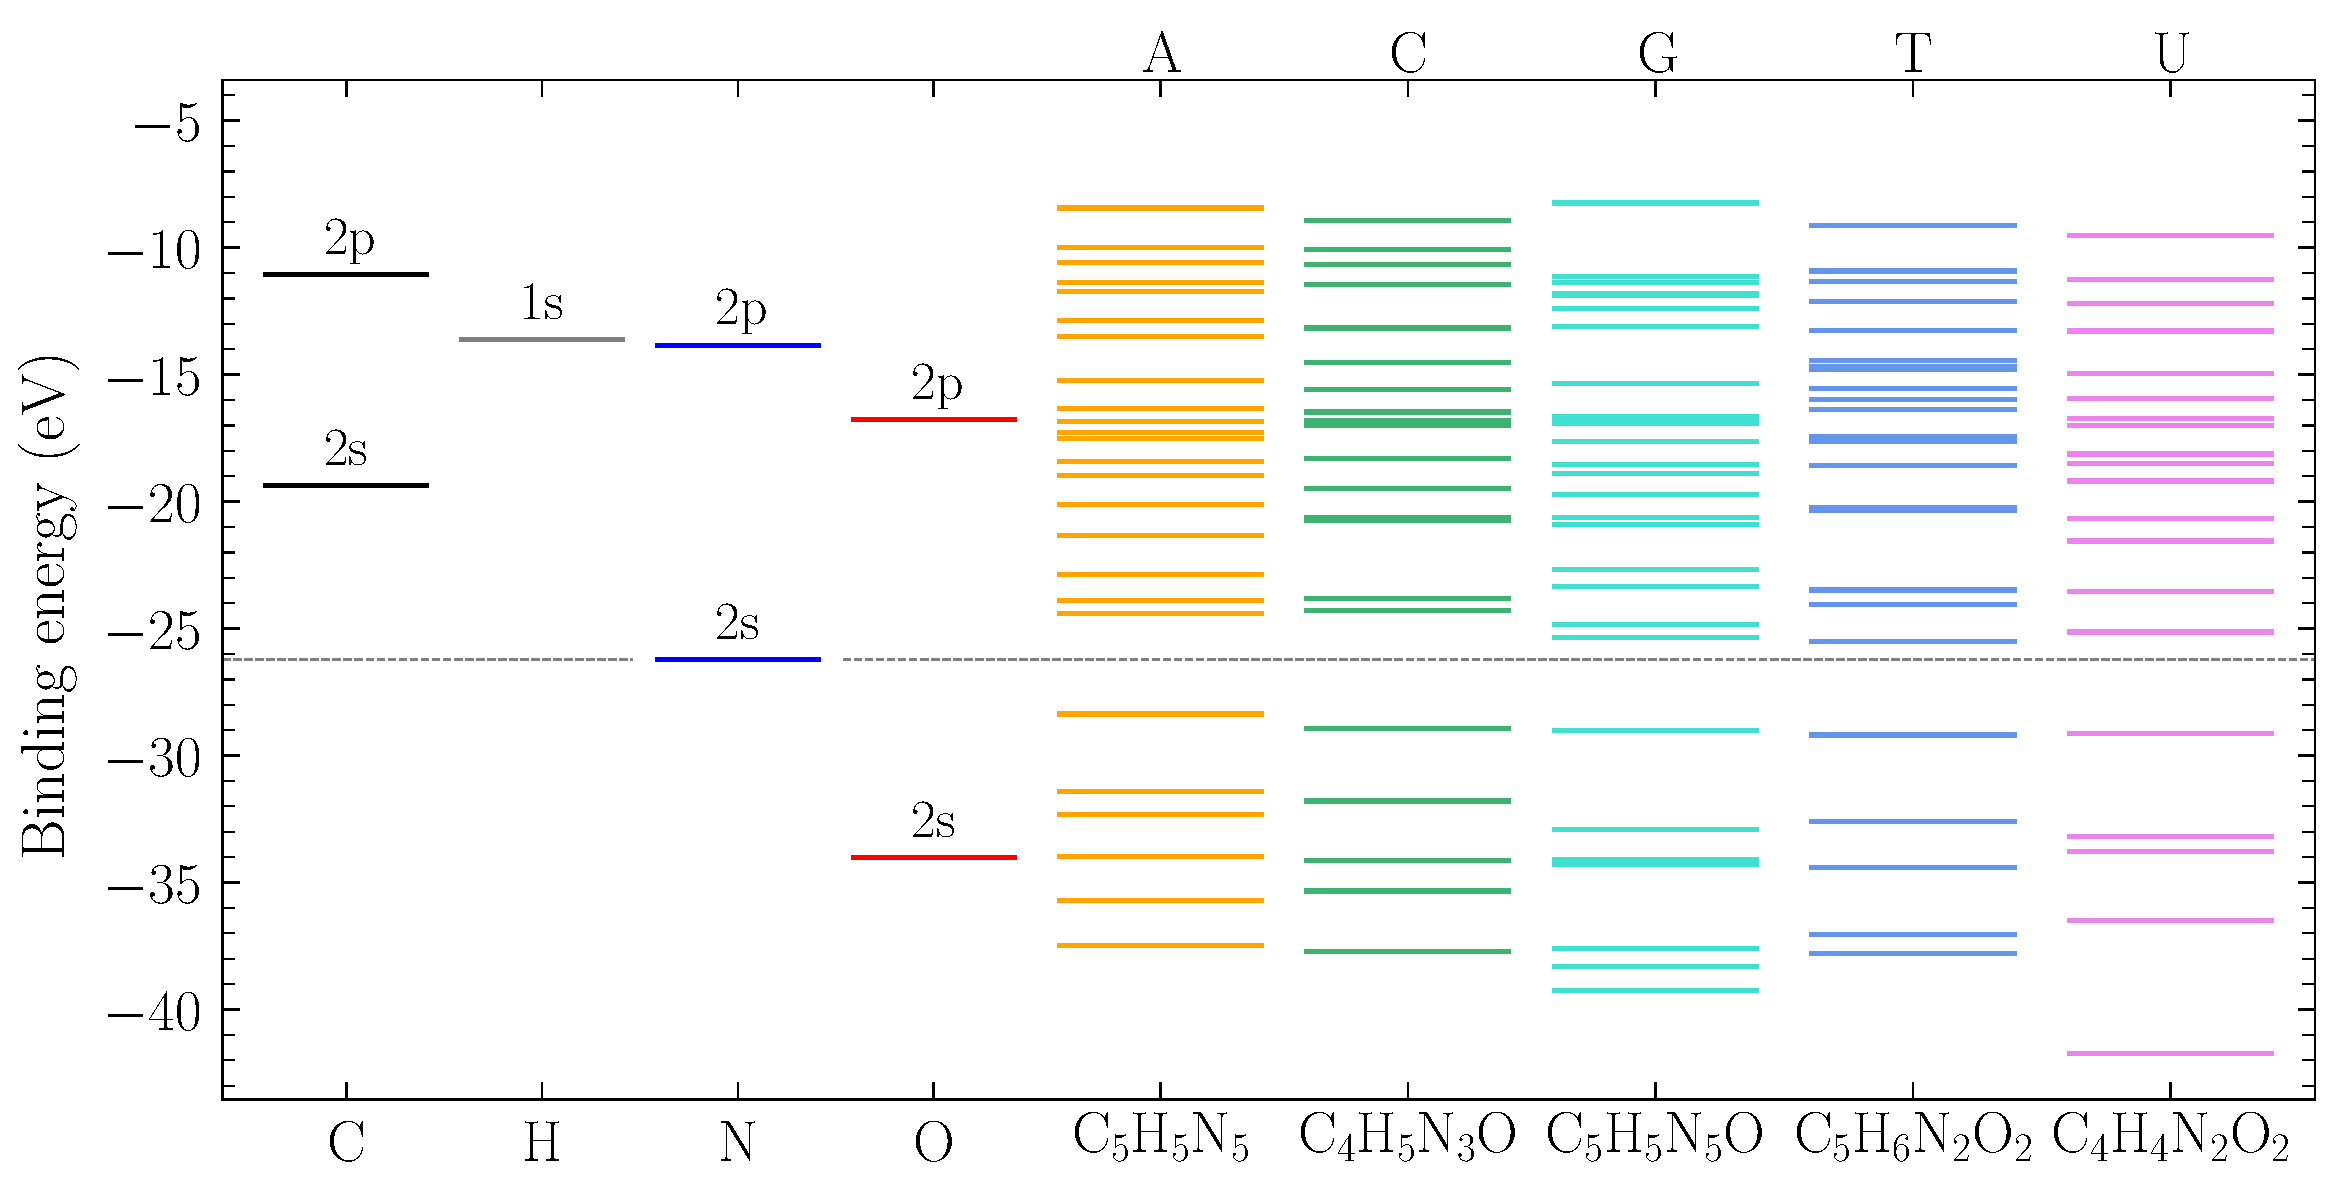
\includegraphics[width=0.9\textwidth]{ionmol/levelsDNA.eps}
\caption[Energías de ligadura moleculares teóricas de ADN y ARN.]
{Energías de ligadura moleculares teóricas de adenina, citosina, guanina, 
timina, y uracilo, comparado con los valores correspondientes de los 
átomos que las constituyen.}
\label{fig:bindener}
\end{figure}

En la Fig.~\ref{fig:bindener} se muestran las energías de ligadura 
molecular de los electrones de valencia para las nucleobases: adenina, 
citosina, guanina, timina y uracilo. Las energías de ligadura del orbital 
molecular más alto (HOMO) obtenidos concuerdan con los valores 
experimentales~\cite{Hush,Verkin,Dougherty} en un 2\% para todas las 
moléculas consideradas. En la izquierda de la Fig.~\ref{fig:bindener}, 
mostramos las energías atómicas de Hartree-Fock de los elementos 
constituyentes. Esta comparación nos da una idea de la distribución de 
los electrones débilmente ligados en las moléculas. Se traza una línea 
discontinua alrededor de $-26$~eV para separar la banda molecular en dos. 
Podemos considerar los niveles de energía atómica por encima de esta 
línea como los correspondientes a los electrones débilmente ligados de la 
Ec.~(\ref{eq:neCDW}). Por ejemplo, los electrones $2s$ y $2p$ del 
carbono se ubican por encima de la línea discontinua, que corresponde a 
los cuatro electrones dados por los números CDW. En el caso de O, solo 
los cuatro electrones de los orbitales 2p se encuentran por encima de la 
línea divisoria propuesta, que se corresponde con el número de electrones
débilmente ligados dado por el escaleo CDW. El caso del átomo de N no es 
tan directo; el número $\nu_{N}^{\text{CDW}}=4$ sugiere que sólo uno de 
los dos electrones de la capa $2s$ contribuye al esquema molecular.

%%%%%%%%%%%%%%%%%%%%%%%%%%%%%%%%%%%%%%%%%%%%%%%%%%%%%%%%%%%%%%%%%%%%%%%%
\subsection{Un modelo estequiométrico modificado}
%%%%%%%%%%%%%%%%%%%%%%%%%%%%%%%%%%%%%%%%%%%%%%%%%%%%%%%%%%%%%%%%%%%%%%%%

El modelo estequiométrico propuesto en la Sección~\ref{sec:SSM} considera 
a la molécula $M$ como un conjunto de átomos neutros aislados, lo cual es 
definitivamente irreal. Una primera mejora se puede sugerir asumiendo que 
los átomos no son efectivamente neutrales y que tienen una distribución 
dispar de los electrones dentro de la molécula. Esta característica puede 
expresarse mediante una carga efectiva $q_{\alpha}$ por átomo. La carga 
de Mulliken proporciona un valor posible para $q_{\alpha}$; sin embargo, 
existe una gran variedad de posibles distribuciones de 
carga~\cite{lee2003}.

\begin{table}
\begin{center}
\begin{tabular}{|p{0.12\textwidth}|p{0.08\textwidth}|p{0.08\textwidth}|p{
0.08\textwidth}|p{0.08\textwidth}|p{0.28\textwidth}|}
\hline
Molécula & C & H & N & O & Estequiometría de carga \\
\hline
Adenina & +0.32 & +0.23 & --0.55 &       & 
C$_{4.92}$H$_{4.77}$N$_{5.14}$ \\ 
\hline
Citosina & +0.28 & +0.21 & --0.56 & --0.53 & 
C$_{3.93}$H$_{4.79}$N$_{3.14}$O$_{1.13}$ \\ 
\hline
Guanina & +0.46 & +0.20 & --0.58 & --0.36 & 
C$_{4.89}$H$_{4.80}$N$_{5.15}$O$_{1.09}$ \\ 
\hline
Timina & +0.20 & +0.19 & --0.54 & --0.52 & 
C$_{4.95}$H$_{5.81}$N$_{2.13}$O$_{2.13}$ \\ 
\hline
Uracilo & +0.31 & +0.22 & --0.59 & --0.47 & 
C$_{3.92}$H$_{3.78}$N$_{2.15}$O$_{2.12}$ \\ 
\hline
\end{tabular}
\caption[Cargas efectivas medias de Mulliken por átomo]
{Cargas efectivas medias de Mulliken por átomo $q_{\alpha}$, y nueva formula
estequiométrica definida por la ecuación~(\ref{eq:newstoi}) para cinco
moléculas de ADN.}
\label{tab:newstoi}
\end{center}
\end{table}

Para tomar en cuenta este efecto, consideramos que el número total de 
electrones $Q_{\alpha }$ en el elemento $\alpha$ se distribuye de forma
dispar sobre todos los átomos $\alpha$. Por lo tanto, cada elemento  
$\alpha$ tendrá una carga $q_{\alpha}=Q_{\alpha}/n_{\alpha}$, que puede 
ser positiva o negativa. Este valor dependerá de la electronegatividad 
relativa respecto a los otros átomos~\cite{rappe1991}. Siguiendo esta 
idea, podemos estimar el número fraccional de átomos por molécula 
$n_{\alpha}'$, el cual está dado por 
\begin{equation}
n_{\alpha }^{\prime }=n_{\alpha }-
\frac{q_{\alpha }}{\nu_{\alpha }^{\text{CDW}}}
\label{eq:newstoi}
\end{equation}
En el caso de átomos neutrales, $q_{\alpha}=0$ y $n_{\alpha}'=n_{\alpha}$,
como dispone el SSM. En la Tabla~\ref{tab:newstoi}, mostramos un valor 
promedio de carga efectiva por átomo $q_{\alpha}$ de C, H, N, y O, para 
cinco moléculas del ADN, las cuales se obtuvieron a partir de los 
cálculos de estructura molecular descritos en la sección anterior.

Implementando la Ec.~(\ref{eq:newstoi}), es posible determinar una nueva 
fórmula estequiométrica de carga, la cual se da en la última columna de 
la Tabla~\ref{tab:newstoi}). Ahora, en vez de tener un número entero de 
átomos $n_{\alpha}$, tenemos un número fraccional dado por $n_{\alpha}'$. 
Se pueden calcular nuevas secciones eficaces moleculares, 
$\sigma'_{M}=\sum_{\alpha}n_{\alpha}'\sigma_{\alpha}$ considerando tales 
valores. Se calcularon errores relativos de las secciones eficaces de 
ionización para las bases de ADN de la Tabla~\ref{tab:newstoi}. Las 
diferencias obtenidas fueron menores de 3\%, lo cual indica que el modelo 
estequiométrico es un modelo robusto con el que se pueden modelar este 
tipo de moléculas complejas dentro del margen de error esperado.

%%%%%%%%%%%%%%%%%%%%%%%%%%%%%%%%%%%%%%%%%%%%%%%%%%%%%%%%%%%%%%%%%%%%%%%%
\section{Conclusiones}
%%%%%%%%%%%%%%%%%%%%%%%%%%%%%%%%%%%%%%%%%%%%%%%%%%%%%%%%%%%%%%%%%%%%%%%%

En este capítulo, hemos estudiado la ionización de blancos moleculares 
de interés biológico debido al impacto de iones de carga múltple. Se han
calculado secciones eficaces de ionización de gran número de blancos 
moleculares de interés biologico conteniendo H, C, N y O por el impacto 
de antiprotones, H$^{+}$, He$^{2+}$, Be$^{4+}$, C$^{6+}$, y O$^{8+}$. 
Nuestras prediciones teóricas han sido obtenidas combinando la 
implementación del método de onda continua distorsionada con estado 
inicial de Eikonal para blancos atómicos (descritos con potenciales 
efectivos DIM), para modelar el proceso colisional, y el modelo 
estequiométrico simple, para aproximar la estructura de las moléculas. 
Presentamos secciones eficaces de ionización total para adenina, 
citosina, timina, guanina, uracilo, THF y agua, siendo comparadas a su 
vez con datos experimentales disponibles. 

Estudiamos y calcularon valores medios de energía y ángulo de emisión de 
los electrones ionizados de blancos atómicos, que son de importancia en 
el daño secundario de las colisiones con iones. Nuestros resultados 
muestran una clara dependencia de estos valores con la carga del ion $Z$. 
Para un blanco dado, a medida que $Z$ aumenta, $\overline{E}_{\alpha}$ 
también aumentan. Por otro lado, $\overline{\theta}_{\alpha}$ decrece, lo 
que muestra una clara tendencia a la dirección del ion. A energía de 
impacto mayores a 2~MeV/amu, estos valores convergen a la primera 
aproximación de Born, la cual establece la simple ley de escala $Z^{2}$. 

Propusimos tres reglas de escala para las secciones eficaces de 
ionización para blancos de interés biológico por cuatro iones desnudos. 
Primero, exploramos la ampliamente usada regla de escala de Toburen, que 
escala la sección eficaz de ionización molecular con un determinado 
número de electrones débilmente ligados. Luego, a partir de los 
resultados CDW para los atómos H, C, N y O, encontramos que la respuesta 
de las secciones eficaces de ionización puede ser optimizada 
normalizándolas con diferentes números de electrones activos en la 
colisión. Así, definimos la primera regla de escala con el número de 
electrones activos CDW, la cual provee buenos resultados para los 
sistemas proyectil--molécula estudiados aquí. La comparación con los 
datos experimentales refuerza nuestros hallazgos. Además, probamos la 
regla de escala CDW mediante la inclusión de datos experimentales de 
ionización de H$_2$, metano y amoníaco por impacto de protones, los 
cuales muestran una buena concordancia en el rango de energías 
intermedias a altas. La segunda regla de escala propuesta considera el 
ion incidente, reduciendo la naturaleza del proyectil mediante el escaleo 
de la sección eficaz de ionización con la carga del ión, $Z^{\alpha}$, 
como una función de la energía incidente reducida $E/Z^{2-\alpha}$, 
siendo $\alpha=1.2$. La última regla que proponemos combina el escaleo de 
la sección eficaz de ionización total con el número de electrones activos 
CDW y la reducción con la carga del ión, $Z^{\alpha}$, lo cual conduce a 
una ley de escala independiente de la carga del ion y el blanco 
molecular. Las tres reglas de escala obtenidas mediante nuestro modelo 
SSM--CDW para los 80 sistemas colisionales examinados fueron comparadas 
con datos experimentales disponibles. Luego, la generalidad de nuestra 
regla de escala independiente fue inspeccionada mediante la inspección
de un número significativo de datos experimentales para otros sistemas 
colisionales (no considerados previamente), probando ésta ser válida 
incluso para energías fuera del rango de validez del método SSM--CDW.

Finalmente, realizamos cálculos de estructura molecular para las 
nucleobases del ADN. Al inspeccionar las energías de ligadura moleculares 
obtenidas mediante cálculos mecanicocuánticos de primeros principios, 
pudimos comprender el número de electrones resultantes de la optimización 
basada en los cálculos CDW. Intentamos mejorar el modelo estequiométrico 
utilizando la carga de Mulliken para obtener proporciones fraccionarias 
en lugar de enteras para el número de átomos constituyentes. No 
encontramos una corrección sustancial, lo que indica que el SSM funciona 
bastante bien. Los presentes resultados refuerzan la exactitud del modelo 
estequiométrico simple y la aproximación CDW para tratar la ionización de 
moléculas complejas por el impacto de iones cargados en el rango de 
energía intermedia a alta. 


\chapter{Pérdida de energía de iones en elementos pesados}

%%%%%%%%%%%%%%%%%%%%%%%%%%%%%%%%%%%%%%%%%%%%%%%%%%%%%%%%%%%%%%%%%%%%%%%%
\section{Introducción}
%%%%%%%%%%%%%%%%%%%%%%%%%%%%%%%%%%%%%%%%%%%%%%%%%%%%%%%%%%%%%%%%%%%%%%%%
\label{sec:intro}

El estudio de procesos de pérdida de energía por impacto de iones 
en sólidos es una poderosa herramienta en diversas áreas de la ciencia
básica y tecnología de materiales. Para energías de impacto superiores 
a unos pocos keV/amu, las partículas cargadas monoenergéticas que 
penetran algún material pierden su energía a través de una serie de 
colisiones inelásticas consecutivas, principalmente con blancos
electrónicos~\cite{Chu:01,Sigmund:06}. La información proporcionada por 
el proceso de pérdida de energía es esencial no solo para tener una 
mejor comprensión de la física detrás de las interacciones fundamentales, 
sino también porque juega un papel fundamental en muchos campos 
aplicados como la ciencia de materiales, la física nuclear, la 
implantación iónica y la radioterapia~\cite{Sigmund:06,Schardt:10}. 
Tablas y códigos resultantes de cálculos semiempíricos están disponibles 
para una gran combinación de iones y objetivos~\cite{iaea_codes,Paul:03}. 
Sin embargo, datos experimentales y predicciones teóricas 
\textit{ab initio} son de crucial importancia para comprobar la 
fiabilidad de los modelos semiempíricos y determinar ciertos 
parámetros clave~\cite{Diwan:15,Damache:04,Damache:02} para la pérdida 
de energía media de iones por trayecto unitario $S(E)$. Los datos 
experimentales disponibles son a menudo bastante escasos para materiales 
correspondientes a elementos de baja presencia en la corteza superior de 
la Tierra. Por otro lado, los cálculos de dispersión inelástica de 
blancos pesados a partir de métodos basados en primeros principios 
constituyen una difícil tarea ya que resulta necesario tener en cuenta 
efectos relativistas. Estos efectos son importantes no sólo para definir 
el estado de los electrones internos sino también para determinar las 
energías de ligadura de las capas externas.

En este capítulo, examinaremos la estructura atómica de blancos pesados
y el proceso de pérdida de energía de iones cuando inciden sobre ellos.
El método de Dirac--Fock (\acs{df}) es quizás la aproximación más 
conocida para el cálculo de funciones radiales y energías orbitales de 
átomos relativistas. Esta aproximación se basa en el principio 
variacional y puede producir resultados muy precisos. Sin embargo, el 
principio variacional presenta varios inconvenientes: el precio de la 
precisión del método se paga con funciones de onda radiales dependientes 
de los términos, las cuales no son ortogonales entre configuraciones. 
Estas características hacen que el uso de las funciones de onda sea 
engorroso en el cálculo las transiciones radiativas y de colisión. Más 
aún, dado que el principio variacional implica la minimización de la 
energía total, las energías de transición entre niveles cercanos se 
obtienen como diferencias muy pequeñas entre números grandes, y los 
resultados son muy susceptibles a errores numéricos. Esto es 
especialmente importante para los átomos pesados porque la energía total 
es muy grande. 

La aproximación teórica que se implementa aquí para describir los 
blancos relativistas fue desarrollada por Klapisch y colaboradores 
\cite{Klapisch:77,Koenig:72,Klapisch:71,Klapisch:67}. En este método, 
el Hamiltoniano multielectrónico de Dirac se resuelve a partir de la 
combinación de la teoría de perturbaciones y la aproximación de campo 
central. La ecuación de Dirac se resuelve y se obtienen las funciones 
de onda de orden cero. El Hamiltoniano resultante es luego diagonalizado 
en las bases de estas funciones implementando el método de interacción 
de configuraciones~(\acs{ci}). El término de Breit y los efectos 
electrodinámicos cuánticos (\acs{qed}) se incluyen a las energías como
correcciones de segundo orden. La descripción 
precisa de los blancos relativistas requiere la optimización de las 
configuraciones definidas; es necesario considerar solo aquellas que 
influyen de manera significativa en el CI. 
{\color{red} Poner algo sobre que el número de configuraciones es 
limitado porque sino todo se desmadra.} 
Las funciones de onda y energías relativistas obtenidas se implementan
luego para describir el blanco en el cálculo de pérdida de energía. La 
correcta descripción de blancos pesados que cuentan con electrones en la 
capa $4f$ es particularmente importante ya que estos electrones tiene un 
rol fundamental en la predicción de pérdida de energía a energías 
bajas~\cite{Roth:17}. 

El enfoque teórico considerado para el cálculo de pérdida de energía 
implementa la aproximación de plasma local por capa (\acs{slpa}) 
\cite{Montanari:13} para describir la energía transferida a los 
electrones ligados $1s$-$4f$ y dos modelos diferentes para el gas de 
electrones libre (\acs{feg}); en la región de baja energía, el modelo 
de potencial apantallado con condición de cúspide (\acs{spcc}) 
\cite{Montanari:17}, que está basado en un formalismo binario no lineal, 
y el formalismo dieléctrico de Mermin-Lindhard (\acs{dielectric-ml}) 
\cite{Mermin:70} para energías alrededor del frenado máximo y 
superiores. Este modelo requiere conocer las funciones de onda 
relativistas y energías de ligadura del blanco, considerando un cierto 
número de electrones de las capas externas en el FEG~\cite{Mendez:19}. 
% El hafnio es particularmente interesante ya que la subcapa 4f (con 14 electrones) es el principal contribuyente por debajo del FEG, lo que hace que las secciones eficaces de frenado sean muy sensibles a una buena descripción de esta capa. Se ha considerado el apantallamiento entre los electrones 4f y 5p y se ha descubierto que juega un papel importante en los cálculos de SLPA.

En este capítulo estudiaremos tres grupos de átomos de la tabla 
periódica: lantánidos con la capa $4f$ abierta (Gd y Er) y metales de 
transición pesados con la capa $4f$ completa (Hf y Pt). 
{\color{red} Escribir sobre las aplicaciones de los blancos que voy a 
tratar: Gd, Er, Hf y Pt  (ver paper de Moro).}

%So far, only one experimental work has been published regarding the stopping power cross section of pure hafnium for protons~\cite{Sirotinin}, while more attention has been recently given to studies involving hafnium oxide due to its practical use~\cite{Abril,Behar,Primetzhofer,Roth}. It is well known that significant attention has been paid in recent years to transition metal-oxides such as HfO$_2$ because of their potential as alternative gate dielectrics to replace SiO$_2$ for the future generation of nano-electronics with less than 45 nm gate length~\cite{Choi,Robertson}. Some important physical properties of the above mentioned metal-oxide films depend on their thickness, which is often measured by using Rutherford Backscattering Spectrometry~\cite{Alfassi01,Tesmer01}. This method relies on the determination of both the scattering cross section and also the stopping power of ion beams in the material of interest.

%In this study, we report experimental stopping power cross sections over the incident energy range (0.6-2.5) MeV for protons crossing self-supported Hf thin-film by using the transmission method. We aim not only to upgrade stopping power data compilations~\cite{HPaul03,mondim17} but also to provide useful information about the processes governing the slowing down of protons in multi-electronic targets. In the rare earth metals, the $4f$ electrons play an essential role in the stopping power since they belong to the first shell of bound electrons below the conduction band. As already noted \cite{Roth17}, the free electron gas (FEG) shows unexpected behavior in these elements, which casts doubts on its proper description. In the case of Hf, we found the contribution of the $4f$-shell to be decisive even at impact energies around the stopping maximum, as will be shown later.

Los detalles teóricos del cálculo de los blancos relativistas a estudiar 
se dan en la sección~\ref{sec:method-target}. Los modelos teóricos 
implementados para la predicción de la pérdida de energia se detallan en 
la sección~\ref{sec:method-stopping}. Los resultados de este trabajo se 
presentan en la sección~\ref{sec:results-heavy}. Las descripciones 
obtenidas para los blancos Gd, Er, Hf y Pt a partir de la 
resolución de la ecuación de Dirac en forma perturbativa se muestran y 
discuten en la sección~\ref{subsec:results-target}. 
Las energías de enlace resultantes se comparan con valores 
experimentales~\cite{Williams:95} y con la descripción dada por 
Desclaux mediante el método de Dirac--Fock~\cite{Desclaux:73}. 
Las predicciones de pérdida de energía obtenidas por nuestro modelo en 
los blancos pesados seleccionados se muestran y discuten la
sección~\ref{subsec:results-stopping}. Se realizan comparaciones con los 
modelos teóricos de Grande y Schiwietz~\cite{Grande:01,casp52}, y de 
Sigmund y Schinner~\cite{DPASS20}. Debido a su gran implementación en 
diversas aplicaciones, también se consideran los valores semi-empiricos 
dados por el paquete SRIM-2013~\cite{Ziegler01} y las tablas 
ICRU-49~\cite{ICRU49}. Las conclusiones de nuestro trabajo se encuentran 
al final del capítulo, en la sección~\ref{sec:conclu-heavy}.

%%%%%%%%%%%%%%%%%%%%%%%%%%%%%%%%%%%%%%%%%%%%%%%%%%%%%%%%%%%%%%%%%%%%%%%%
\section{Descripción de blancos relativistas}
%%%%%%%%%%%%%%%%%%%%%%%%%%%%%%%%%%%%%%%%%%%%%%%%%%%%%%%%%%%%%%%%%%%%%%%%
\label{sec:method-target}

La descripción de los estados de átomos pesados relativistas se 
obtiene resolviendo el Hamiltoniano multielectrónico de 
Dirac~\cite{Klapisch:77,Koenig:72,Klapisch:71,Klapisch:67}
\begin{equation}
 H = H' + H_{\mathrm{\mbox{\scriptsize Breit}}}(i,j) +
 H_{\mbox{\scriptsize QED}}\,,
\label{eq:htot}
\end{equation}
donde $H_{\mathrm{\mbox{\scriptsize Breit}}}(i,j)$ es el término de 
Breit, $H_{\mbox{\scriptsize QED}}$ considera los efectos 
electrodinámicos cuánticos (\acs{qed}), y
\begin{equation}
 H' = \sum_i \left[ h_i^{\mbox{\scriptsize D}} - \frac{Z}{r_i}\right]
 + \sum_{i<j}\frac{1}{r_{ij}}\,,
\label{eq:HDirac}
\end{equation}
siendo $h_i^{\mbox{\scriptsize D}}$ el término cinético del 
Hamiltoniano de Dirac de una partícula. Los términos restantes en la
ecuación~(\ref{eq:hprim}) corresponden a las interacciones 
núcleo--electrón y electrón--electrón, respectivamente. Usando la 
aproximación de campo central y mediante la introducción de un potencial 
paramétrico $U(\boldsymbol{\alpha},r)$, el Hamiltoniano $H'$ se puede escribir como la 
combinación de un término de orden cero, 
\begin{equation}
 H_0 = \sum_i h_i^{\mbox{\scriptsize D}} + U(\boldsymbol{\alpha},r_i)\,,
\end{equation}
más una pequeña perturbación
\begin{equation}
 H_1 = \sum_{i<j}\frac{1}{r_{ij}}
 - \sum_i \left[ \frac{Z}{r_i} + U(\boldsymbol{\alpha},r_i) \right]\,.
\end{equation}
Las soluciones de espinor de cuatro componentes de un electrón de la 
ecuación de Dirac
\begin{equation}
\left[ h_i^{\mbox{\scriptsize D}} +U(\boldsymbol{\alpha},r) \right] \varphi_{nljm}(\mathbf{r}) 
= \varepsilon_{nljm} \varphi_{nljm}(\mathbf{r})\,,
\label{eq:ecuacionDirac}
\end{equation}
llamadas orbitales relativistas, pueden ser caracterizadas por un 
conjunto de números cuánticos $nljm$, donde $l$ es el número cuántico 
del momento angular orbital de las componentes superiores. 
% componentes superiores = upper components ???

La solución de orden cero de un sistema $N$--electrónico se construye a 
partir de productos antisimetrizados de orbitales en cualquier esquema 
de acoplamiento elegido $\Gamma JM$ como 
\begin{equation}
\Psi_{\Gamma}\left(\mathbf{r}_1, \mathbf{r}_2, \ldots, \mathbf{r}_N\right)=A \sum_{all\,\,m}\left\langle\Gamma J M \mid m_1 m_2, \ldots, m_{N}\right\rangle \prod_{a} \varphi_{n_a l_a j_a m_a}\left(\mathbf{r}_a\right)\,,
\end{equation}
donde $A$ es el operador de antisimetría. Los estados y niveles 
específicos se denotan $\Gamma_iJ_iM_i$ y $\Gamma_iJ_i$, respectivamente,
donde $\Gamma_i$ representa el conjunto de números cuánticos necesario 
para identificar el estado de manera únivoca. 

Una configuración 
$C\equiv\prod_{a=1}^N\mathbf{j}_a=\prod_{i=1}\mathbf{j}_i^{q_i}$ es un 
conjunto de estados degenerados, con valores fijos $\mathbf{j}_i=n_il_ij_i$
y números de ocupación $q_i$, todos con energías de orden cero 
$E_C^0=\prod_{i=1}\,q_i\varepsilon_i$. 
El Hamiltoniano $H'$ se construye sobre la base de las configuraciones 
elegidas obtenidas con el potencial paramétrico. Luego, la matriz es 
diagonalizada, produciendo estados de configuración mixtos y energías 
de primer orden con algunas correcciones de correlación. Las funciones 
de onda resultantes se utilizan para agregar las correcciones QED y el 
término de Breit a las energías como perturbaciones de segundo orden.

La idea detrás del potencial paramétrico $U(\boldsymbol{\alpha},r)$ es 
describir de manera simple el apantallamiento de la distribución de carga 
de los electrones usando una expresión paramétrica analítica, donde 
$\boldsymbol{\alpha}=\left\{\alpha_1,\alpha_2,\ldots,\alpha_k\right\}$ 
es un conjunto de parámetros que se definen mediante la optimización 
del sistema y $k$ es el número de capas ocupadas. Aplicando la ecuación de 
Poisson a la densidad de carga radial de los $q$ electrones descritos 
por los orbitales de tipo Slater
\begin{equation}
\rho(r) = -4\pi r^2 qN\left|r^{l+1}e^{-\alpha r/2}\right|^2\,,
\end{equation} 
con las condiciones de borde 
\begin{equation}
U(\boldsymbol{\alpha},r\rightarrow\infty)=Z-\frac{q}{r}\,.
\end{equation} 
Aquí, $N$ es un factor de normalización, y $\alpha_i$ está relacionado 
con el radio medio de la capa tal que $\alpha_i=(2l+3)/\langle r\rangle_i$. 
Es necesario mostrar que el potencial para diversas capas y el nucleo 
se puede escribir como
\begin{equation}
U(\boldsymbol{\alpha},r)=-\frac{1}{r} \left[I+\sum_s q_s\, g(L_s,\alpha_s,r) 
+ \sum_t q_t\,f(l_t,\alpha_t,r)\right]\,,
\label{eq:potparam}
\end{equation}
donde los índices $s$ y $t$ recorren las capas cerradas y abiertas, 
respectivamente. El valor $I$ es el grado de ionización más uno. 
%Esto elimina la auto-interacción adicional de los electrones ligados. Aquí, $\boldsymbol{\alpha}$ representa un conjunto de parámetros $\left\{\alpha_s,\alpha_t\right\}$ que describen el radio medio de las capas. 
Las funciones $f$ y $g$ son tales que
\begin{eqnarray}
f(l,\alpha,r)&=&\mathrm{e}^{-\alpha r} \sum_{j=1}^{2 l+1}\left(1-\frac{j}{2 l+2}\right) \frac{(\alpha r)^{j}}{j !}\,, \\
g(L, \alpha, r)&=&\frac{1}{2 n^{2}} \sum_{l=0}^{L=n-1}(4 l+2) f\left(l, \alpha^{(l)}, r\right)\,,
\end{eqnarray}
donde $n$ es el número cuántico principal y $\alpha^{(l)}$ incluye una
corrección para la ligera diferencia en el radio debido al número del
momento angular cuántico de las subcapas. 
Los parámetros libres $q$ son el número efectivo de electrones en la 
capa y satisfacen $I+\sum_{s} q_{s}+\sum_{t} q_{t}=Z$. 

Esta parametrización resulta en que cualquier cantidad atómica calculada 
con las funciones de onda dadas por la ecuación~(\ref{eq:ecuacionDirac}) 
junto con el potencial~(\ref{eq:potparam}) se convierte en una función 
numérica de los parámetros. Hay múltiples formas posibles de elegir los 
parámetros $\boldsymbol{\alpha}$, de acuerdo a diversos criterios 
teóricamente válidos. Entre ellos, podemos nombrar tres;
\begin{itemize}
\item criterio espectroscópico: minimización de la desviación \acs{rms} 
entre los niveles de energía teóricos y experimentales,
\item criterio variacional: minimización de la energía total, y
\item criterio perturbacional: minimización del Hamiltoniano perturbativo
$H_1$. 
\end{itemize}
En nuestro trabajo, implementamos la minimización de las energías de 
configuración promedio (\acs{ca}), o de las energías de cualquier 
conjunto de niveles elegido. Dado que las energías de primer orden sobre 
las que actúa la optimización incluyen la contribución de intercambio 
exacta, los parámetros resultantes absorben el efecto del intercambio y, 
por lo tanto, no hay necesidad de un potencial de intercambio adicional 
explícito.

%la optimización de los blancos se realiza resoviendo la ecuación de Dirac a primer orden,

Por otro lado, siendo $U(\boldsymbol{\alpha},r)$ un potencial central,
es posible plantear la separación de variables esféricas de las 
soluciones de la ecuación de Dirac~(\ref{eq:ecuacionDirac}), tal que
\begin{equation}
\varphi_{nljm}(\mathbf{r}) = \frac{1}{r} \left( 
\begin{array}{c}
i P_{nlj}(r) \,\Omega_{jlm}(\hat{\mathbf{r}}) \\ 
  Q_{nlj}(r) \,(\boldsymbol{\sigma}\cdot\hat{\mathbf{r}})\,\Omega_{jlm}(\hat{\mathbf{r}})
\end{array}
\right)\,,
\label{eq:sepespinor}
\end{equation}
donde $P_{nlj}(r)$ y $Q_{nlj}(r)$ son los componentes fuerte y débil de los 
espinores de Dirac, respectivamente. Los espinores esféricos 
$\Omega_{jlm}(\hat{\mathbf{r}})$ son autoestados de $J^2$ y $J_z$ a 
través de la relación
\begin{equation}
\Omega_{j, l, m}(\theta, \phi)=\sum_{\mu} C(l, 1 / 2, j ; m-\mu, \mu, m) Y_{l, m-\mu}(\theta, \phi) \chi_{\mu}\,,
\end{equation}
donde $C\left(j_{1}, j_{2}, j ; m_{1}, m_{2}, m\right)$ son los
coeficientes de Clebsch--Gordan. Así, el valor esperado de cualquier 
operador $\hat{A}$ estará dado por
\begin{equation}
\langle\hat{A}\rangle=\int_0^{\infty}\left[P^*(r)\,\hat{A}\,P(r) 
 +Q^*(r)\,\hat{A}\,Q(r)
\right]\,dr\,.
\label{eq:meanvalr}
\end{equation}
Para los orbitales relativistas, usamos la notación $nl\pm$, que 
significa $nlj$, donde el índice $j=l\pm1/2$ se representa como $\pm$.

%%%%%%%%%%%%%%%%%%%%%%%%%%%%%%%%%%%%%%%%%%%%%%%%%%%%%%%%%%%%%%%%%%%%%%%%
\section{Modelo teórico de pérdida de energía}
%%%%%%%%%%%%%%%%%%%%%%%%%%%%%%%%%%%%%%%%%%%%%%%%%%%%%%%%%%%%%%%%%%%%%%%%
\label{sec:method-stopping}

La pérdida de energía de iones en blancos metálicos responde a diferentes
mecanismos físicos, dependiendo de la velocidad del proyectil incidente.
A bajas velocidades, las colisiones binarias son responsables de la 
pérdida de energía. La contribución principal es la ionización de los 
electrones de la banda de conducción del metal, que está aproximada por 
un gas de electrones libres (FEG) de velocidad de Fermi $v_F$. Por arriba
de un valor particular de velocidad (i.e., $v\geq 1.5\,v_F$), no solo 
ocurren excitaciones binarias sino también colectivas (plasmones) 
\cite{Montanari:17}. Más aún, a altas energías, los electrones ligados
también contribuyen al potencial de frenado. El método teórico de 
pérdida de energía combina una descripción de FEG para la interacción del
proyectil con los electrones de valencia (o conducción) y una 
aproximación diferente para la interacción con los electrones ligados.

Usamos el modelo de potencial apantallado con condición de cúspide 
(\acs{spcc})~\cite{Montanari:17} para describir el potencial de frenado 
de partículas cargadas con bajas velocidades de impacto en el FEG. Este 
método está basado en la aproximación de colisión binaria no 
perturbativa, de manera que es válida para valores de energías menores a 
las excitaciones de plasmones. La SPCC está basada en un potencial 
centrado apantallado con una condición de cúspide para la densidad 
electrónica cerca del proyectil. Este modelo ha probado dar buenas 
descripciones para la densidad de electrones inducida, aún para 
proyectiles con carga negativa. Además, este modelo predice correctamente 
las diferencias entre protón-antiprotón en el potencial de frenado, más 
conocido como el efecto Barkas. El formalismo SPCC depende sólo del radio 
de Wigner-Seitz $r_S$, que es una medida de la densidad electrónica del 
FEG. Para metales de $r_S$ conocidos, el SPCC describe correctamente los 
valores experimentales del potencial de frenado a bajas energías, en 
concordancia con resultados DFT de Echenique y 
colaboradores~\cite{Echenique:81,Nagy:89} a $v=0$.

Por encima de cierta velocidad de impacto, la contribución del plasmón 
es esencial (alrededor del máximo de la sección eficaz de frenado). Un 
valor de interés para nuestro análisis es la velocidad de impacto mínima 
para excitar plasmones, $v_P$. En el formalismo dieléctrico, este valor 
se puede obtener como $v_P\,\approx\,v_F[1+(3\pi\,v_F)^{-1/2}]$
\cite{suppression}. Para describir la pérdida de energía considerando la 
excitación colectiva y binaria, se recurre al formalismo dieléctrico de 
Mermin-Lindhard (ML)~\cite{Mermin:70}, que es una aproximación 
perturbativa de respuesta lineal, por lo que depende del cuadrado de la 
carga del proyectil. En este formalismo, la respuesta de los electrones 
del blanco al paso de iones se describe a través de la función 
dieléctrica cuántica, que depende de los parámetros característicos 
$r_S$ y $\delta$ del FEG.

La potencia de frenado debido a los electrones ligados se obtiene 
empleando la aproximación de plasma local por capa 
(SLPA)~\cite{Montanari:17,Montanari:13}. Vale la pena destacar que las 
únicas cantidades de las cuales depende este modelo son las densidades 
radiales orbitales del estado fundamental y sus energías de enlace. El 
modelo incluye los procesos colectivos y el apantallamiento entre 
electrones. 

Para la contribución de los electrones ligados a la sección eficaz de 
frenado total, el método de SLPA considera las contribuciones 
independientes de cada subcapa. Nuestras energías de ligadura 
relativistas presentan un desdoblamiento de espín-órbita. Sin embargo, 
en la potencia de frenado total, donde el estado inicial del electrón 
excitado no es medido, la incertidumbre cuántica en energía $\Delta E$ 
fusiona el desdoblamiento. El criterio $\Delta E\Delta t\geq\hbar/2$ une 
las energías $E_{nl+}-E_{nl-}$ para valores de tiempos medios de colisión
$\Delta t$ lo suficientemente pequeños. De hecho, a una velocidad de 
impacto suficientemente alta, podemos esperar que todos los electrones 
del blanco respondan juntos al paso de los 
iones~\cite{Lindhard:53,Chu:72}. Siguiendo trabajos 
previos~\cite{Montanari:09}, el tiempo de colisión se estima como 
$\Delta t\approx\langle r_i\rangle/v$, siendo $\langle r_i\rangle$ y $v$ 
el radio orbital medio y la velocidad de impacto, respectivamente. 
%En el caso del hafnio, encontramos que para cada subcapa de electrones, la división espín-órbita no se resuelve en la región de energía a la que contribuye esta subcapa. Por lo tanto, los nl-electrones deben considerarse juntos, respondiendo al paso de iones como un solo gas de electrones con densidad $\delta_{nl}(r)$ y energía de enlace media $E_{nl}$. Esta característica es vital dentro de los cálculos de SLPA porque explica el filtrado entre electrones de la misma energía de enlace.

%%%%%%%%%%%%%%%%%%%%%%%%%%%%%%%%%%%%%%%%%%%%%%%%%%%%%%%%%%%%%%%%%%%%%%%%
\section{Resultados}
%%%%%%%%%%%%%%%%%%%%%%%%%%%%%%%%%%%%%%%%%%%%%%%%%%%%%%%%%%%%%%%%%%%%%%%%
\label{sec:results-heavy}

En esta sección presentamos los resultados obtenidos de la optimización
de ciertos blancos relativistas y su implementación en el estudio de 
procesos de pérdida de energía tales como la potencia de frenado y la 
ionización de electrones de la capa $L$.

%%%%%%%%%%%%%%%%%%%%%%%%%%%%%%%%%%%%%%%%%%%%%%%%%%%%%%%%%%%%%%%%%%%%%%%%
\subsection{Energías de ligadura y valores medios}
%%%%%%%%%%%%%%%%%%%%%%%%%%%%%%%%%%%%%%%%%%%%%%%%%%%%%%%%%%%%%%%%%%%%%%%%
\label{subsec:results-target}

Los efectos de la interacción de configuraciones (\acs{ci}) son muy 
importantes en el caso de los átomos relativistas. Así, la correcta 
descripción del blanco depende de las configuraciones consideradas en 
el CI. En esta sección, la optimización de los blancos consiste en la 
determinación de las configuraciones que contribuyen de manera 
significativa a la mezcla en la interacción de configuraciones. 

El Hamiltoniano perturbativo de Dirac, dado por la 
ecuación~(\ref{eq:HDirac}), de los blancos relativistas a describir se 
resuelve aplicando el método perturbativo descrito anteriormente. Por 
simplicidad, llamamos a este método Dirac perturbativo (PD). Las 
soluciones numéricas se obtienen usando el paquete de códigos 
{\sc hullac}~\cite{BarShalom:01}. En este conjunto de programas 
computacionales, el código {\sc relac} permite calcular las energías 
relativistas y funciones de onda orbitales en primer orden. 

\begin{table*}[t]
\centering
\begin{tabular}{|c|c|c|c|l|}
\hline
Nombre   & Símbolo & $Z$ & Config. fundamental & Serie \\
\hline
\hline
Gadolinio & Gd & 64 & [Xe]~$4f^7\,5d\,6s^2$ & \multirow{2}{*}{Lantánidos} \\
Erbio     & Er & 68 & [Xe]~$4f^{12}\,6s^2$ & \\
\hline
Hafnio  & Hf & 72 & [Xe]~$4f^{14}\,5d^2\,6s^2$ & \multirow{2}{*}{Metales de transición}\\
Platino & Pt & 78 & [Xe]~$4f^{14}\,5d^9\,6s$ & \\
\hline
\end{tabular}
\caption[Blancos relativistas y sus configuraciones fundamentales]
{Blancos relativistas: símbolos, cargas nucleares $Z$, configuraciones 
fundamentales y serie.}
\label{tab:gruposrelat} 
\end{table*}

Los elementos que examinamos en esta sección se dividen en dos grupos 
según la serie de la tabla periódica a la que pertenecen. Los blancos a 
estudiar, sus símbolos, carga nuclear $Z$ y configuraciones fundamentales 
se muestran en la tabla~\ref{tab:gruposrelat}. El grupo de lantánidos a
analizar está compuesto por Gd y Er. Los metales de transición Hf y Pt 
conforman el grupo de metales de transición bajo estudio. 

Podemos escribir una fórmula general para la configuración fundamental 
de los lantánidos,
\begin{equation}
nf^w\,(n+1)d^x\,(n+2)s^y\,,
\end{equation}
donde $n=4$, $w=7,12$, $x=1,0$ y $y=2,2$. En el caso de Gd, también 
tenemos que incluir las interacciones entre los electrones de las capas
$4f$ y $5d$, que están abiertas. Así, las contribuciones más 
importantes a la interacción de configuraciones están dadas por la 
mezcla de las configuraciones $4f^7\,5d\,6s^2$ y $4f^8\,6s^2$.
Para Er, la mayor mezcla es producida por las configuraciones 
$4f^{12}\,6s^2$ y $4f^{12}\,5d\,6s$.

Por otro lado, podemos escribir la configuración fundamental de los 
metales de transición en forma general como
\begin{equation}
nd^w\,(n+1)s^x\,,
\end{equation}
donde $n=5$, $w=2,9$, $x=2,1$ para el grupo A. Los electrones $nd$ y 
$(n+1)s$ tienen energías de ligadura similares. Por lo tanto, las 
configuraciones 
\begin{gather}
nd^w(n+1)s^2, \\
nd^{w+1}(n+1)s, \\
nd^{w+2}
\end{gather}
tienen energías comparables. Dado que estas configuraciones tienen la 
misma paridad, éstas cumplen los dos requerimientos mencionados 
anteriormente, y son fundamentales en los cálculos de mezcla de 
configuraciones. Entonces, por ejemplo, para el átomo de Pt, las 
configuraciones [Xe]~$5d^9\,6s$ y $5d^{10}$ son consideradas en el 
cálculo relativista.

%%%%%%%%%%%%%%%%%%%%%%%%%%%%%%%%%%%%%%%%%%%%%%%%%%%%%%%%%%%%%%%%%%%%%%%%
Las energías de ligadura de los blancos relativistas de la 
tabla~\ref{tab:gruposrelat} que se obtienen a partir del método PD se 
dan en la tabla~\ref{tab:relatresults} y se muestran en la 
figura~\ref{fig:bindener} con diamantes rellenos. En la tabla se 
incluyen los valores medios $\langle r\rangle$ de cada capa, los cuales 
se obtienen a partir de la ecuación~(\ref{eq:meanvalr}). Datos 
experimentales de los blancos en estado sólido~\cite{Williams:95} se 
presentan usando círculos vacíos. Los resultados obtenidos por 
Desclaux~\cite{Desclaux:73} mediante la implementación del método 
de Dirac--Fock se muestran en la figura con símbolos $\times$. También 
se incluyen resultados no relativistas mediante la implementación del 
método de Hartree--Fock~\cite{FroeseFischer:97} con símbolos 
$\triangleleft$.

\begin{longtable}{|c|ccc|ccc|}
\caption[Energías de ligadura y valores $\langle r \rangle$ de blancos
relativistas]
{Energías de ligadura teóricas perturbativas y 
experimentales~\cite{Williams:95} de Gd, Er, Hf y Pt. 
Valores medios $\langle r \rangle$ en a.u. obtenidos a partir de la 
ecuación~(\ref{eq:meanvalr}).}
\label{tab:relatresults}\\
\hline
%% primer encabezado
\multirow{2}{*}{$nlj$} 
 & $E^{\mbox{\tiny exp}}$
 & $E^{\mbox{\tiny PD}}$
 & $\langle r\rangle^{\mbox{\tiny PD}}$
 & $E^{\mbox{\tiny exp}}$
 & $E^{\mbox{\tiny PD}}$
 & $\langle r\rangle^{\mbox{\tiny PD}}$ \\
\endfirsthead % fin de primer encabezado
%% segundo encabezado (tabla continuada)
\caption* {(Cont.): Energías de ligadura teóricas perturbativas y 
experimentales~\cite{Williams:95} de Gd, Er, Hf y Pt. 
Valores medios $\langle r \rangle$ en a.u. obtenidos a partir de la 
ecuación~(\ref{eq:meanvalr}).} \\
 \hline
$nlj$ 
 & $E^{\mbox{\tiny exp}}$
 & $E^{\mbox{\tiny PD}}$
 & $\langle r\rangle^{\mbox{\tiny PD}}$
 & $E^{\mbox{\tiny exp}}$
 & $E^{\mbox{\tiny PD}}$
 & $\langle r\rangle^{\mbox{\tiny PD}}$ \\
 \hline
\endhead
\hline
\endfoot
\endlastfoot
  \cline{2-7}
  &  \multicolumn{3}{c}{Gd}  &  \multicolumn{3}{c}{Er} \\
\hline
$1s$   & 1846.2 & 1843.6 & 0.0219 & 2112.7 & 2114.2 & 0.0203 \\
$2s$   & 307.8  & 303.0  & 0.0929 & 358.4  & 353.7  & 0.0858 \\
$2p_-$ & 291.4  & 287.2  & 0.0776 & 340.5  & 337.5  & 0.0712 \\
$2p_+$ & 266.2  & 261.6  & 0.0845 & 307.2  & 303.3  & 0.0785 \\
$3s$   & 69.13  & 67.43  & 0.244  & 81.07  & 79.34  & 0.225  \\
$3p_-$ & 62.03  & 60.79  & 0.234  & 73.72  & 72.00  & 0.215  \\
$3p_+$ & 56.74  & 55.50  & 0.247  & 66.59  & 64.92  & 0.229  \\
$3d_-$ & 44.904 & 44.084 & 0.219  & 53.40  & 51.91  & 0.202  \\
$3d_+$ & 43.717 & 42.953 & 0.223  & 51.78  & 50.38  & 0.207  \\
$4s$   & 13.91  & 13.50  & 0.553  & 16.53  & 15.62  & 0.507  \\
$4p_-$ & 10.5   & 10.9   & 0.565  & 13.46  & 12.69  & 0.515  \\
$4p_+$ & 9.96   & 9.74   & 0.596  & 11.77  & 11.06  & 0.548  \\
$4d_-$ & -      & 5.515  & 0.634  & 6.160  & 6.186  & 0.578  \\
$4d_+$ & 5.240  & 5.306  & 0.645  & 6.160  & 5.892  & 0.589  \\
$5s$   & 1.3    & 2.0    & 1.34   & 1.86   & 1.95   & 1.25   \\
$5p_-$ & 0.74   & 1.3    & 1.51   & 1.15   & 1.16   & 1.41   \\
$5p_+$ & 0.74   & 1.2    & 1.60   & 0.908  & 0.954  & 1.52   \\
$4f_-$ & 0.32   & 0.41   & 0.916  & -      & 0.18   & 0.813  \\
$4f_+$ & 0.32   & 0.38   & 0.934  & 0.17   & 0.14   & 0.838  \\
$6s$   &        & 0.31   & 3.70   &        & 0.19   & 4.33  \\
$5d_-$ &        & 0.29   & 2.50   &        &        &      \\
$5d_+$ &        & 0.28   & 2.56   &        &        &     \\
\hline
& \multicolumn{3}{c}{Hf} & \multicolumn{3}{c}{Pt} \\
\hline
$1s$   & 2401.6 & 2400.4 & 0.0190 & 2880.9 & 2881.6 & 0.0171 \\
$2s$   & 414.20 & 408.98 & 0.0798 & 510.08 & 504.78 & 0.0718 \\
$2p_-$ & 394.65 & 390.26 & 0.0662 & 487.77 & 483.25 & 0.0591 \\
$2p_+$ & 351.4  & 346.4  & 0.0740 & 424.97 & 419.70 & 0.0676 \\
$3s$   & 95.58  & 93.55  & 0.208 & 121.1  & 118.8  & 0.187 \\
$3p_-$ & 86.91  & 85.40  & 0.198 & 111.2  & 109.4  & 0.177 \\
$3p_+$ & 77.43  & 75.97  & 0.213 & 97.20  & 95.37  & 0.192 \\
$3d_-$ & 63.06  & 62.14  & 0.187 & 80.92  & 79.83  & 0.168 \\
$3d_+$ & 61.08  & 60.12  & 0.191 & 77.98  & 76.83  & 0.172 \\
$4s$   & 19.8   & 18.8   & 0.468 & 26.66  & 25.53  & 0.416 \\
$4p_-$ & 16.10  & 15.45  & 0.474 & 22.38  & 21.55  & 0.419 \\
$4p_+$ & 13.99  & 13.28  & 0.508 & 19.09  & 18.22  & 0.453 \\
$4d_-$ & 8.08   & 7.81   & 0.530 & 12.19  & 11.70  & 0.463 \\
$4d_+$ & 7.772  & 7.418  & 0.542 & 11.56  & 11.09  & 0.474 \\
$5s$   & 2.36   & 2.55   & 1.12  & 3.737  & 3.829  & 0.942 \\
$5p_-$ & 1.4    & 1.6    & 1.24  & 2.40   & 2.53   & 1.02 \\
$5p_+$ & 1.10   & 1.28   & 1.35  & 1.90   & 1.94   & 1.12 \\
$4f_-$ & 0.584  & 0.725  & 0.666 & 2.74   & 2.75   & 0.513 \\
$4f_+$ & 0.522  & 0.660  & 0.679 & 2.62   & 2.62   & 0.520 \\ 
$6s$   &        & 0.214  & 3.83  &        & 0.250  & 3.30 \\  
$5d_-$ &        & 0.125  & 2.77  &        & 0.250  & 1.71 \\  
$5d_+$ &        & 0.109  & 3.13  &        & 0.200  & 1.88 \\
\hline
\end{longtable}

\begin{figure}[H]
\centering
\includegraphics[width=\textwidth]{heavy/bindener.eps}
\caption[Energías de ligadura de blancos relativistas]
{Energías de ligadura de Gd, Er, Hf y Pt. Símbolos: 
$\blacklozenge$ resultados teóricos del presente trabajo, 
$\times$ valores teóricos del método Dirac--Fock~\cite{Desclaux:73}, 
$\triangleleft$ valores teóricos según Hartree--Fock, y 
$\medcircle$ datos experimentales en sólidos~\cite{Williams:95}.}
\label{fig:bindener}
\end{figure}

\begin{figure}[t]
\centering
\includegraphics[width=\textwidth]{heavy/ratios_heavy_barh.eps} 
%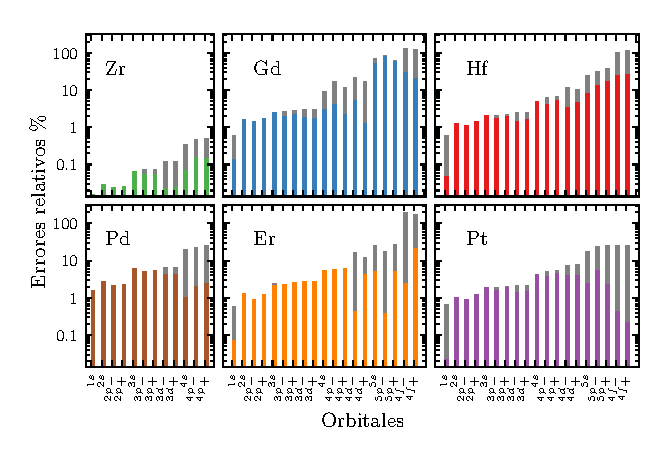
\includegraphics[width=\textwidth]{heavy/erp_heavy.eps} 
\caption[Razón $E^{\mbox{\scriptsize exp}}/E$ entre energías de ligadura 
experimentales y teóricas.]
{Razón $E^{\mbox{\scriptsize exp}}/E$ entre energías de ligadura 
experimentales y teóricas de Gd, Er, Hf y Pt: métodos de Hartree--Fock 
(barras gris oscuro), Dirac--Fock (barras gris claro), y Dirac 
perturbativo (barras de colores).}
\label{fig:ratios}
\end{figure}

Dado que la figura~\ref{fig:bindener} muestra las energías de enlace en 
un rango de magnitud de cinco órdenes, no es posible discernir las 
discrepancias entre los datos experimentales y los resultados teóricos
obtenidos mediante los métodos de Hatree--Fock, Dirac--Fock y Dirac 
perturbativo. Para poder inspeccionar estas diferencias con más detalle, 
las relaciones entre las energías de ligadura experimentales 
$E^{\mbox{\scriptsize exp}}$ y teóricas (HF, DF y PD) se muestran en la 
figura~\ref{fig:ratios}. La figura muestra claramente que las 
correcciones relativistas son críticas para describir la estructura 
atómica de los blancos considerados, incluso para las capas externas. 
Por ejemplo, la energía de enlace no relativista de la subcapa $4f$ de 
Hf es cuatro veces la experimental. Un valor tan incorrecto conduce a la 
subestimación de la ionización de los electrones $4f$ y desplaza el 
umbral a energías más altas. Por otro lado, los valores teóricos 
relativistas de Dirac--Fock mejoran la descripción de las capas internas 
de los blancos de forma sistemática. Sin embargo, las discrepancias con 
los valores experimentales en las capas cercanas a la banda de valencia 
son significativas. En definitiva, la incorrecta descripción de los 
orbitales de las capas internas se propaga a las capas externas en los 
cálculos no relativistas (HF) y relativistas (DF) que implementan el 
método variacional. 

En general, el acuerdo entre nuestros resultados teóricos perturbativos 
relativistas y las mediciones experimentales es muy bueno. 
Las energías de enlace que obtuvimos para los lantánidos muestran un 
acuerdo de aproximadamente 3\%, con excepción de las subcapas más 
externas $5s$, $5p$ y $4f$ del Gd. Asimismo, los resultados 
obtenidos para Hf y Pt coinciden con los valores experimentales en 
$\sim$3\%, excepto en las subcapas $5p$ y $4f$ de Hf. En todos los 
casos, los resultados obtenidos a partir del método perturbativo 
describen los datos experimentales con mayor precisión que los valores 
dados por el método variacional de Hartree--Fock y su versión 
relativista~\cite{Desclaux:73}. En general, el método perturbativo 
permite describir en forma más precisa tanto las capas más internas 
--donde se esperan los efectos relativistas-- como las capas externas.

%%%%%%%%%%%%%%%%%%%%%%%%%%%%%%%%%%%%%%%%%%%%%%%%%%%%%%%%%%%%%%%%%%%%%%%%
\subsection{Electrones en el FEG}
%%%%%%%%%%%%%%%%%%%%%%%%%%%%%%%%%%%%%%%%%%%%%%%%%%%%%%%%%%%%%%%%%%%%%%%%

Las energías de ligadura fueron calculadas considerando los blancos como 
átomos aislados (gases). Sin embargo, las energías 
experimentales~\cite{Williams:95} consideradas para las comparaciones 
corresponden a mediciones en sólidos (ionización de los electrones 
ligados). Como es de esperar, las principales discrepancias gas-sólido 
se encuentran en las capas externas. Los electrones en las órbitas 
adyacentes a la banda de conducción en un sólido están débilmente 
ligados, en comparación con los electrones en un átomo aislado. Las 
líneas verticales discontinuas de la figura~\ref{fig:bindener} separan 
los electrones ligados de los de valencia. Los presentes resultados dan 
una buena idea sobre el número de electrones en el gas de electrones 
libres (FEG) de los sólidos, que son particularmente relevantes en los 
cálculos de potencia de frenado.

El FEG está caracterizado por la densidad de electrones o, 
equivalentemente, por el radio de Wigner-Seitz, $r_S$. A su vez, éstos 
se encuentran directamente relacionados con la energía de Fermi, $E_F$. 
Para obtener estos valores y determinar el número real de electrones que 
pertenecen al FEG, es necesario realizar un análisis exhaustivo de las 
energías de ligadura. Nuestros resultados teóricos para cada blanco se 
presentan en la tabla~\ref{tab:electronFEG}. Para Hf, el valor 
experimental de $r_S$ se deriva de la función de pérdida de energía 
óptica~\cite{Lynch:75,Isaacson:75}, lo que resulta en 
$r_S^{\mbox{\scriptsize exp}}=2.12$. Nuestros resultados teóricos 
acuerdan con estos valores en menos del 4\%. A nuestro saber, no hay 
valores experimentales para los átomos de Gd y Er. Mientras que para Pt, 
el número de electrones en el FEG está sujeto a discusión. 
Por ejemplo, si se suponen 6 electrones en la banda de valencia (parte 
de los electrones $5d$), la energía de Fermi que se obtiene es 
$E_F=0.72$~a.u.. Por otro lado, si se considera toda la subcapa de 
valencia $d$ en la banda de conducción, el valor correspondiente es 
$E_F=1.02$~a.u..

\begin{table}[t]
\centering
\begin{tabular}{|c|c|c|c|c|}
\hline
Símbolo & $Z$ & $N_e$ & $r_S$ & $E_F$ \\
\hline
\hline
Gd & 64 & 10 & 1.75 & 0.602 \\
Er & 68 & 14 & 1.52 & 0.792 \\
\hline
Hf & 72 & 4  & 2.14 & 0.40 \\
Pt & 78 & 10 & 1.34 & 1.02 \\
\hline
\end{tabular}
\caption[Parámetros teóricos de FEG para blancos relativistas.]
{Parámetros teóricos de FEG propuestos para Gd, Er, Hf y Pt: 
carga nuclear $Z$, número de electrones en el FEG $N_e$, radio de 
Wigner--Seitz $r_S$ y energía de Fermi $E_F$.}
\label{tab:electronFEG} 
\end{table}

Para los átomos estudiados aquí, notamos que las energías de enlace de 
los electrones más externos se encuentran debajo de las energías de 
Fermi. Sin embargo, las curvas inferiores de la figura~\ref{fig:bindener} 
muestran un claro contraste entre los lantánidos y el resto de átomos. 
Para Gd, la tabla~\ref{tab:electronFEG} muestra que los electrones $4f$ 
tienen energías muy cercanas a las subcapas exteriores $5d$ y $6s$. Esta 
característica nos lleva a considerarlos como parte de la FEG. Se llega 
a la misma conclusión para Er. Como se dijo anteriormente, la 
determinación específica de las capas de valencia y subvalencia son 
importantes en la física del estado sólido. En particular, admitir los 
electrones $4f$ en el FEG permite explicar las principales características 
de las mediciones recientes~\cite{Montanari:17,Montanari:19} de baja 
energía de la potencia de frenado de protones en Gd~\cite{Roth:17}.


%%%%%%%%%%%%%%%%%%%%%%%%%%%%%%%%%%%%%%%%%%%%%%%%%%%%%%%%%%%%%%%%%%%%%%%%
\subsection{Potencial de frenado}
%%%%%%%%%%%%%%%%%%%%%%%%%%%%%%%%%%%%%%%%%%%%%%%%%%%%%%%%%%%%%%%%%%%%%%%%
\label{subsec:results-stopping}

%%%%%%%%%%%%%%%%%%%%%%%%%%%%%%%% Hafnio %%%%%%%%%%%%%%%%%%%%%%%%%%%%%%%%

\begin{figure}[H]
\centering
\includegraphics[width=\textwidth]{heavy/Hf_methods.eps}
\caption[Secciones eficaces teóricas de frenado de protones en Hf.]
{Secciones eficaces teóricas de frenado de protones en hafnio.
Frenado debido al FEG: método no perturbativo SPCC (línea discontinua 
celeste) y formalismo dieléctrico de ML (línea sólida celeste). 
Frenado debido a los electrones ligados $1s$-$4f$: método SLPA con (línea 
sólida verde) y sin (línea punteada verde) apantallamiento de las 
subcapas $5p$-$4f$. 
Las curvas totales (líneas rojas) resultan de sumar las contribuciones 
del FEG y los electrones ligados. 
%Línea discontinua: método SPCC (FEG) y SLPA (electrones ligados). 
%Líneas sólida: ML (FEG) y SLPA (electrones ligados) con apantallamiento. 
%Línea punteada: ML (FEG) y SLPA (electrones ligados) sin apantallamiento.
La línea vertical punteada indica el valor de energía (37 keV) en el cual 
las excitaciones de plasmones pueden ocurrir.} 
\label{fig:Hf_methods}
\end{figure}

\begin{figure}[H]
\centering
\includegraphics[width=\textwidth]{heavy/Hf_RNR.eps}
\caption[Secciones eficaces relativistas y no relativistas de Hf.]
{Secciones eficaces teóricas con descripción relativista y no relativista
del blanco. Símbolos: valores experimentales.}
\label{fig:Hf_SP}
\end{figure}

\begin{figure}[H]
\centering
\includegraphics[width=\textwidth]{heavy/Hf_interp.eps}
\caption[Interpolación de sección eficaz de frenado total.]
{Interpolación de sección eficaz de frenado total de Hf. Símbolos:
método no perturbativo SPCC (FEG) + SLPA (electrones ligados) con 
círculos; formalismo dieléctrico de ML (FEG) + SLPA (electrones ligados) 
con cuadrados.} 
\label{fig:Hf_interp}
\end{figure}

\begin{figure}[H]
\centering
\includegraphics[width=\textwidth]{heavy/Hf_SPall.eps}
\caption[Secciones eficaces teóricas, semiempíricas y experimentales de 
Hf.]{Secciones eficaces de frenado total teóricas, semiempíricas y
experimentales de Hf.}
\label{fig:Hf_SP}
\end{figure}

%%%%%%%%%%%%%%%%%%%%%%%%%%%%%%% Platino %%%%%%%%%%%%%%%%%%%%%%%%%%%%%%%%

\begin{figure}[H]
\centering
\includegraphics[width=\textwidth]{heavy/Hf_methods.eps}
\caption[Secciones eficaces teóricas de frenado de protones en Pt.]
{Secciones eficaces teóricas de frenado de protones en platino.
Frenado debido al FEG: método no perturbativo SPCC (línea discontinua 
celeste) y formalismo dieléctrico de ML (línea sólida celeste). 
Frenado debido a los electrones ligados $1s$-$5s$ con apantallamiento de 
las subcapas $5p$-$4f$ usando el método SLPA (línea sólida verde).
Las curvas totales (líneas rojas) resultan de sumar las contribuciones 
del FEG y los electrones ligados. 
%Línea discontinua: método SPCC (FEG) y SLPA (electrones ligados). 
%Líneas sólida: ML (FEG) y SLPA (electrones ligados) con apantallamiento. 
La línea vertical punteada indica el valor de energía (39.4 keV) en el 
cual las excitaciones de plasmones pueden ocurrir.} 
\label{fig:Pt_methods}
\end{figure}

\begin{figure}[H]
\centering
\includegraphics[width=\textwidth]{heavy/Pt_SPall.eps}
\caption[Secciones eficaces teóricas, semiempíricas y experimentales de 
Pt.]{Secciones eficaces de frenado total teóricas, semiempíricas y
experimentales de Pt.}
\label{fig:Pt_SP}
\end{figure}


%%%%%%%%%%%%%%%%%%%%%%%%%%%%%%%%%%%%%%%%%%%%%%%%%%%%%%%%%%%%%%%%%%%%%%%%
\subsection{Ionización de capa L}
%%%%%%%%%%%%%%%%%%%%%%%%%%%%%%%%%%%%%%%%%%%%%%%%%%%%%%%%%%%%%%%%%%%%%%%%
\label{subsec:results-ionLshell}

\newpage
%%%%%%%%%%%%%%%%%%%%%%%%%%%%%%%%%%%%%%%%%%%%%%%%%%%%%%%%%%%%%%%%%%%%%%%%
\section{Conclusiones}
%%%%%%%%%%%%%%%%%%%%%%%%%%%%%%%%%%%%%%%%%%%%%%%%%%%%%%%%%%%%%%%%%%%%%%%%
\label{sec:conclu-heavy}

Binding energies and wave functions were computed for several atoms
having nuclear charges ranging between 41 and 78, by solving the
fully--relativistic Dirac equation with the set of codes {\sc hullac}, 
which includes the Breit term and QED corrections. The agreement between 
the present theoretical results and the experimental values is excellent,
with the sole exception of the subvalence shells of some transition
elements. The present results are found to be closer to the experimental 
ones than other theoretical computations. 
The fact that the theoretical calculations have been performed
for isolated atoms, and
the experimental values correspond to binding energies of solids,
accounts for the differences encountered. 
Our results allow to propose theoretical Wigner--Seitz radii for all 
the targets. We found a particular feature for the lanthanides, which
indicates that the $4f$ electrons belong to the free electron gas.


\begin{comment}

%=======================================================================
\section{Experimental arrangements}
\label{experiment}

%-----------------------------------------------------------------------
\subsection{Accelerator and scattering Chamber}
The procedure used in this work to obtain stopping power data is 
essentially the same as described in Ref.~\cite{Miranda01}. The present 
measurements were made at the IST/LATR (Laboratory of Accelerators and 
X-Ray Diffraction) in Lisbon. This facility uses a 2.5 MV Van de Graaff 
accelerator to deliver $^1$H$^+$ primary ion beams with a precision better 
than $\pm 0.5$ keV through a series of electrostatic lenses and collimators 
onto a thin Au/SiO$_2$ sample, which is used as a scattering center. The Hf 
foil was mounted on a movable target holder and placed inside a RBS/C scattering 
chamber to allow energy measurements of the direct beam and the beam transmitted 
through the sample without breaking the high vacuum ($\sim$10$^{-6}$ Torr) inside 
the scattering chamber. The beam current on the sample was kept at around 5.0 nA 
to attain sufficient statistics in each particle spectrum. By using a beam spot 
of about 1.0 mm in diameter, a solid angle of 11.4 msr was attained. The overall 
energy resolution (FWHM) of the detection system was about 15 keV relative to 5.486 
MeV alpha particles from a $^{241}$Am source.

%-----------------------------------------------------------------------
\subsection{Target}
The stopping material under analysis was a hafnium foil with a nominal 
thickness of 1.0 $\mu$m and 99.95\% purity, which was supplied by Lebow 
Company~\cite{Lebow}. A more precise thickness value was achieved by measuring 
the energy loss of alpha particles coming from a calibrated 
($^{239}$Pu, $^{241}$Am, $^{244}$Cm) source. From the alpha 
spectra with and without the Hf foil interposed, the characteristic 
energy shift $\delta$E was measured and then combined with the stopping 
power for 5.486 MeV alphas on hafnium (55.69 eV/$10^{15}$ at/cm$^2$) 
found in Ref.~\cite{Ziegler01} to obtain an areal density of 
($4.13 \pm 0.21$)$\times 10^{19}$ at/cm$^2$, which corresponds to a 
thickness of $0.920\pm0.046 \mu$m. Target non-uniformity was investigated through 
systematic measurements (at five different points over the sample area) of the energy 
loss of alpha particles from the same radioactive source. The uncertainties originating
from the non-uniformity of the sample was $\sim 2.5$\%. However, the primary source of
uncertainty related to target thickness comes from estimates in the SRIM database for 
alphas on hafnium ($\sim$ 4\%). Additionally, we consider estimates coming from surface 
roughness ($\sim$ 1\%) and possible impurities ($\sim$ 1\%) in the foil; and finally, 
statistical uncertainty ($\sim$ 0.6\%) related to the gaussian fits used to determine 
the energy loss of alphas through the Hf target.

%-----------------------------------------------------------------------
\subsection{Energy loss measurement}
%-----------------------------------------------------------------------
\begin{figure}[!t]
\centering
\includegraphics[width=9cm]{Fig01.eps}
\caption{RBS spectrum for $E_{\mathrm{avg}}=921.1$ keV protons on 
hafnium sample which is subsequently used to determine the energy loss 
in the foil.}
\label{F01}
\end{figure}

Once the beam impinges on the Au/SiO$_2$ sample, protons are 
backscattered towards a Si surface barrier detector located at 
140$^{\circ}$ relative to the initial beam direction. Fig.~\ref{F01} 
shows two particle spectra, where the ion energies $E_2$ and $E_1$ are 
associated with a placed and removed hafnium sample, respectively. Both 
energy distributions were fitted by Gaussian functions to obtain the 
mean energy and width (FWHM) of the peaks \cite{Sun01}, and from the 
difference between these two peak positions in the spectrum, the total 
energy loss $\Delta E = (E_1 - E_2)$ in the foil was calculated. As 
established in previous studies \cite{Miranda01,Damache02}, the 
experimental stopping power cross sections $\varepsilon (E) $ are 
determined at some mean energy $E_{\mathrm{avg}}$ by measuring the ion 
energy losses $\Delta E$ within the investigated Hf foil, which has a 
mean thickness denoted by $\Delta x$. In this way, only when the energy 
loss fraction $\Delta E/E_{\mathrm{avg}}$ across the Hf foil is not 
exceeding 20\%, it is possible to define the stopping cross section by 
\cite{Raisanen01,Schulz01}:
\begin{equation}\label{eq:stcross}
 \varepsilon(E)=\frac{S(E)}{N}=-\frac{dE}{N\,dx}\approx-\frac{\Delta E}{N\Delta x},
\end{equation}
where $N$ denotes the atomic number density (atoms cm$^{-3}$) of the 
material under study. When this condition was not fulfilled, a small 
correction to the mean energies $E_{\mathrm{avg}}$ was applied in order 
to account for the non-linear dependence on ion energy of stopping powers 
\cite{Chilton,Rajatora}. The uncertainty ($\sim$ 0.7\%) in the measured energy 
loss $\Delta E$ of protons in the hafnium sample is mainly related to the 
statistical uncertainty found in the gaussian fits mentioned above. If this value 
is combined with the $\sim$ 4.9\% uncertainty in target thickness, then a 
$\sim$ 5.0\% uncertainty in the measured cross section is obtained.

%=======================================================================
\section{Pérdida de energía} 

Hafnium ($Z=72$, [Xe] $4f^{14}\,6s^2\,5d_{3/2}^1\,5d_{5/2}^1$) belongs 
to the first groups of transition metals, with four electrons as FEG 
($r_S=2.14$ a.u.) and $1s$-$4f$ electrons bound. We compared the 
computed $r_S$ with the experimental value obtained from the measured 
energy loss function by Lynch \textit{et al.}~\cite{lynch75}. The 
experimental plasmon energy of Hf is $\hbar\omega_P \approx 15.8$ eV, 
with a width at half maximum $\delta\approx 4.4$ eV, and 
$r_S\approx 2.07$ a.u.~\cite{lynch75}. The difference of less than 
$5\%$ between theoretical and experimental $r_S$ assess Hf as a 
canonical target~\cite{mon17}.

%----------------------------------------------------------------------
\begin{figure*}[!t]
\centering
\includegraphics[width=11.cm]{stopping/bindener.eps}
\caption{(a) Binding energies of Hf. Present relativistic and available 
non-relativistic~\cite{badnell97} values are given with filled symbols. 
Experimental measurements for solids~\cite{williams1995} are depicted 
with open circles. (b) Corresponding relative errors respect to 
experimental data.}
\label{Binding_E}
\end{figure*}
%------------------------------------------------------------------------

To assess the importance of a fully relativistic description of bound 
electrons, Fig.~\ref{Binding_E}~(a) shows our binding energies, 
$E_{nl\pm}$, with $\pm=j\pm1/2$; non-relativistic values~\cite{badnell97}; 
and experimental data on solid-state Hf~\cite{williams1995}, which is 
available only for $1s$ to $4f_{\pm}$ subshells, as expected. We notice that not only the most inner shells 
require relativistic calculations, but also the outer $5p$ and $4f$ 
shells. Furthermore, this figure shows very clearly the disability of 
non-relativistic calculations to describe the experimental data, which 
surprisingly worsens from the inner to the outer shells.

From the comparison with the experimental values in Fig.~\ref{Binding_E}~(a),
it can be noted that the sign of the binding energy deviations is 
inverted for the outer $5s$ and $4f$ electrons, with the experimental 
binding energies being less bounded than our theoretical ones. Small 
differences for the outer shells are expected since the experimental
values correspond to hafnium in solid-state, while our theoretical 
calculations correspond to the element in the gas phase.

More detail about the theoretical binding energies is given in 
Fig.~\ref{Binding_E}~(b), where relative errors with respect to the 
experimental values are shown. This figure shows clearly that the 
relativistic corrections are critical to describe the atomic structure 
of hafnium, even for the outer shells. It turns out that the errors 
committed in the non-relativistic calculations of the inner shell 
orbitals propagate, through the Hartree-Fock approximation, to the outer 
shells. 
The non-relativistic $4f$ binding energy is four times the experimental one. Such an incorrect value leads to the underestimation of the $4f$-ionization and shifts  the threshold to higher energies.  
The importance of fully relativistic calculations for the outer 
shells has already been noted for Au, Pb, Bi, and W~\cite{mon09}.

For example, the $4f_{-}$ and $4f_{+}$ of Hf can only 
be resolved for impact energies $E<0.05$ keV, but the contribution of 
$4f$ to the total stopping is negligible for $E<40$ keV. Moreover, the 
$5p$ and $4f$ electrons of Hf are very close in energy 
($\Delta E_{5p-4f} \approx 1$ a.u.~\cite{mendez2019}), and they react 
together at impact energies $E>40$ keV (inter-shell screening). As 
already mentioned, at higher energies, inter-shell screening is also possible 
for deeper subshells %(i.e., $4p$-$4d$ for impact energies above 0.9 MeV), 
but their weight in the total stopping is minor.

Finally, in all our calculations~\cite{mon17}, we assumed the projectile 
to be proton and not neutral hydrogen. When an ion moves inside a metal, 
the FEG screens the nucleus, so the binding energies will be smaller 
than outside the metal, and this effect is more critical at low impact 
velocities $v$. In the case of hydrogen, the difference is drastic, 
i.e., for H inside Hf ($rs=2.07$), the $1s$-bound state is almost null at 
$v<2$~\cite{suppression}. It is worth to mention that this assumption 
agrees with Ziegler SRIM code~\cite{Ziegler01} but differs from CasP 
code~\cite{Grande}, that predicts neutral hydrogen at very low velocities.

%-----------------------------------------------------------------------
\begin{figure*}[!t]
\centering
\includegraphics[width=13.0cm]{stopping/Fig03_new2.eps}
\caption{(color online) Stopping power cross section of hafnium for 
protons. Symbols: solid circles, present values; open circles, previous 
data~\cite{Sirotinin}. Curves: 
Black solid-line, present full theoretical results with $4f$-$5p$ screening; 
pink dash-dot line, theoretical CasP5.2~\cite{Grande,casp52} values; 
orange dash-double-dot line, theoretical DPASS~\cite{DPASS20} results; 
green dotted-line, semi-empirical SRIM-2013~\cite{Ziegler01}; 
violet dashed-line, ICRU49~\cite{ICRU49} tabulated values.}
\label{F03}
\end{figure*}
%-----------------------------------------------------------------------

In Fig.~\ref{slpa4f}, we display the present theoretical stopping cross
section of Hf for protons using the relativistic wave functions 
and binding energies, but with and without the $5p$-$4f$ screening. 
We show the FEG and bound electron contributions separately and the 
total stopping as the addition of both of them. The minimum energy for 
plasmon excitation was estimated at approximately $37$ keV. We used the 
non-perturbative SPCC model for impact energies $E \leq 37$~keV, and the 
perturbative ML calculation above this value. Bound $1s$-$4f$ electrons 
(relativistic wave functions and binding energies) are calculated with 
the SLPA and shown separately in Fig.~\ref{slpa4f} with and without the 
$4f$-$5p$ screening. Below $\sim 40$ keV, the difference between both 
calculations is negligible. Considering $5p$-$4f$ electrons 
as a single group of 20 electrons with screening among them gives lower 
stopping values than the addition of the separate $5p$ and $4f$ 
contributions. Notice that this shell correction can only be considered self-consistently within a many-electron model, such as the SLPA.

%=======================================================================
\section{Resultados}
\label{discussion}

The present data are displayed in Table~\ref{table01}. As can be observed, 
an overall relative uncertainty of around 5\% was achieved for the experimental 
stopping power values, which are mainly due to the uncertainty in the hafnium foil 
thickness. 

%-----------------------------------------------------------------------
\begin{table*}[!t]
\centering
\caption{Stopping power values S$_{\mathrm{exp}}$ of hafnium for protons 
measured in this work. $\Delta$E/E values are also shown.}
\label{table01}

\vspace{0.2cm}

%\begin{ruledtabular}
\begin{tabular}{ccc|ccc|ccc} %\hline\hline
E$_{\mathrm{avg}}$ & S$_{\mathrm{exp}}$       & $\Delta$E/E & E$_{\mathrm{avg}}$ & S$_{\mathrm{exp}}$       & $\Delta$E/E & E$_{\mathrm{avg}}$ & S$_{\mathrm{exp}}$       & $\Delta$E/E \\
keV                & eV/(10$^{15}$ at/cm$^2$) & \%          & keV                & eV/(10$^{15}$ at/cm$^2$)	& \%          & keV                & eV/(10$^{15}$ at/cm$^2$) & \% \\ \hline
516.6	 & 25.8	$\pm$	1.3	&	20.5	&	1170.3	&	18.25	$\pm$	0.91	&	6.4	&	1813.4	&	15.10	$\pm$	0.76	&	3.4	\\
567.8	 & 24.8	$\pm$	1.2	&	17.9	&	1220.0	&	18.08	$\pm$	0.90	&	6.1	&	1862.7	&	14.79	$\pm$	0.74	&	3.3	\\
618.8	 & 23.9	$\pm$	1.2	&	15.8	&	1269.6	&	17.57	$\pm$	0.88	&	5.7	&	1912.0	&	14.21	$\pm$	0.71	&	3.0	\\
669.6	 & 23.2	$\pm$	1.2	&	14.2	&	1319.2	&	17.32	$\pm$	0.87	&	5.4	&	1961.2	&	14.46	$\pm$	0.72	&	3.0	\\
720.1	 & 22.5	$\pm$	1.1	&	12.8	&	1368.8	&	17.15	$\pm$	0.86	&	5.1	&	2010.4	&	14.34	$\pm$	0.72	&	2.9	\\
770.5	 & 21.8	$\pm$	1.1	&	11.6	&	1418.3	&	16.69	$\pm$	0.83	&	4.8	&	2059.6	&	13.76	$\pm$	0.69	&	2.7	\\
820.8	 & 21.3	$\pm$	1.1	&	10.7	&	1467.8	&	16.43	$\pm$	0.82	&	4.6	&	2108.8	&	13.78	$\pm$	0.69	&	2.7	\\
871.0	 & 20.8	$\pm$	1.0	&	9.8	&	1517.2	&	16.13	$\pm$	0.81	&	4.4	&	2158.0	&	13.70	$\pm$	0.69	&	2.6	\\
921.1	 & 20.3	$\pm$	1.0	&	9.1	&	1566.7	&	16.04	$\pm$	0.80	&	4.2	&	2206.5	&	13.33	$\pm$	0.67	&	2.5	\\
971.1	 & 19.9	$\pm$	1.0	&	8.4	&	1616.0	&	15.77	$\pm$	0.79	&	4.0	&	2256.4	&	13.27	$\pm$	0.66	&	2.4	\\
1021.0 & 19.33	$\pm$	0.97	&	7.8	&	1665.4	&	15.51	$\pm$	0.78	&	3.8	&	2305.5	&	13.07	$\pm$	0.65	&	2.3	\\
1070.8 & 19.03	$\pm$	0.95	&	7.3	&	1714.8	&	15.46	$\pm$	0.77	&	3.7	&	2354.7	&	12.91	$\pm$	0.65	&	2.2	\\
1120.6 & 18.73	$\pm$	0.94	&	6.9	&	1764.1	&	14.93	$\pm$	0.75	&	3.5	&	2403.8	&	12.61	$\pm$	0.63	&	2.2	\\ \\ 
\end{tabular}
%\end{ruledtabular}
\end{table*}

Fig.~\ref{F03} synthesizes the results of the present work. The 
agreement between the present theoretical results and the new 
measurements displayed in Table~\ref{table01} is excellent. Present 
measurements using the transmission method are in good agreement with 
the previous data by Sirotinin~\cite{Sirotinin}, which were measured 
in backscattering geometry. Our theoretical approach also agrees with 
the data by Sirotinin~\cite{Sirotinin}, except for the lowest energy 
measurement at 80 keV. We have also included in this figure the 
theoretical curves from the CasP5.2 code by Grande and 
Schiwietz~\cite{Grande,casp52} and from the DPASS code by Sigmund and 
Schinner~\cite{DPASS20}, both available online. Furthermore, we 
incorporated the semi-empirical results from SRIM-2013~\cite{Ziegler01} 
and the ICRU49 tables~\cite{ICRU49}. Interestingly, our full theoretical 
curve differs from SRIM-2013 for impact energies below 100 keV. We 
obtain a stopping maximum of approximately 
$40\times 10^{-15}$ eV cm$^2$/atom at 65 keV. Instead, following the 
up-to-now only set of data \cite{Sirotinin}, SRIM-2013 suggests a lower 
stopping maximum at an impact energy of 115 keV. 

The stopping maximum is 
a very sensitive region for any full theoretical description, and this is quite visible in a linear-scale plot like 
Fig.~\ref{F03}. However, the impact energy for the maximum seems to 
agree between our curve and DPASS, although it is $10 \%$ below. 
Instead, CasP maximum is $10 \%$ above ours, but 
has a completely different shape at lower energies. It is worth 
mentioning that our model gives similar results using the experimental 
value $r_S=2.07$ a.u. rather than the theoretical one $r_S=2.14$ a.u.,
with the stopping maximum at the same impact energy but $4\%$ higher. Future experiments would be important for a more complete understanding of this case, mainly for proton energies around the stopping maximum (i.e. $30-300$ keV) and also below $25$ keV, in the region where a linear dependence with the velocity is expected.


%=======================================================================
\section{Conclusiones}
\label{sec:stopping-conclusiones}

In this work, we have used the transmission method to experimentally 
determine stopping power cross section values for (0.6-2.5) MeV protons 
incident on self-supporting Hf foils with an overall uncertainty of 
around 5\%. Additionally, we calculated values extracted from the 
theoretical framework that involved the relativistic wave functions and 
binding energies of Hf and considered four electrons per atom in the 
free electron gas. The shell-wise local plasma approximation was 
employed to describe the energy transferred to the bound $1s$-$4f$ 
electrons, and two different models for the FEG: the screened potential 
with cusp condition (SPCC model) for energies below that of the plasmon 
excitation, and the Mermin-Lindhard dielectric formalism, for energies 
around the stopping maximum and above. Present theoretical stopping 
cross sections cover an extensive energy range from 1 keV/amu to 
10 MeV/amu.

At high impact energies, the new stopping  measurements are in good 
agreement with our theoretical results, with previous experimental data
and semi-empirical values by SRIM-2013 and ICRU-49.  However, we call 
the attention that around the stopping maximum and at lower impact 
energies, the difference between our full-theoretical results and SRIM 
is substantial. We compare our theoretical results with two other models 
given by the DPASS and CasP5.2 codes. Differences can be noted at 
intermediate to low impact energies, but they also support a stopping 
maximum at lower energy than SRIM predictions. 

To the best of our knowledge, these are the first theoretical 
calculations of stopping in Hf that cover from very low to high impact energies, taking into account relativistic effects in the atomic structure and screening among electrons in a consistent 
way. Future experiments for 
impact energies around the stopping maximum and in the low energy region 
would be essential to have a better understanding of the stopping of 
protons in hafnium.

\end{comment}




\chapter{Excitación por impacto de electrones: la optimización bayesiana}
\label{chap:bayeopt}

\begin{comment}

Como no estas poniendo nada relacionado a Powell, me imagino que
este dio bien y no te queres echar tierra. Si no es asi, es
necesario que expliques como se hace hoy, y que estas proponiendo
para mejorarlo.

Luego, podes explicar la optimizacion Bayesiana (o lo mandas a un apendice),
recalcando que no estas optimizando una funcion matematica (por mas
que en este caso, si lo estes haciendo...).
Finalmente, van los resultados, pero con graficos que sean mas claros.
Los que vi son demasiado especificos, demasiado tecnicos y engorrosos.

Tenes que explicar un poquito la forma de la seccion eficaz,
o del collision strength, explicar que son esas resonancias,
cual es la forma que se espera obtener, que cosa esta bien y
que mal, y que tan dificil es llegar a estos resultados.

Finalmente, el estilo de escritura es de receta de cocina.
No es una lista de actividades. Es un relato. Acompaña al lector,
llevalo por las diferentes ideas, creale un interes, una
tension, mas misterio y mas poesia. (!)

\end{comment}

%%%%%%%%%%%%%%%%%%%%%%%%%%%%%%%%%%%%%%%%%%%%%%%%%%%%%%%%%%%%%%%%%%%%%%%%
\section{Introducción}
%%%%%%%%%%%%%%%%%%%%%%%%%%%%%%%%%%%%%%%%%%%%%%%%%%%%%%%%%%%%%%%%%%%%%%%%
\label{sec:intro}

El análisis de observaciones espectroscópicas es la única herramienta 
disponible para el diagnóstico de plasmas astrofísicos y de laboratorio. 
El modelado e interpretación de dichas observaciones requiere de una 
extensa variedad de datos de estructura atómica. Los cálculos de niveles 
de energía de átomos y sus iones son utilizados como guía para 
identificar las líneas espectrales observadas, mientras que sus 
intensidades requieren la determinación de secciones eficaces 
colisionales y probabilidades de transición. El modelo 
colisional-radiativo resultante precisa de coeficientes de tasa de 
diversos procesos. En particular, la excitación por impacto de 
electrones determina en gran medida la distribución de la población 
emisora dentro de un estado de carga. Existe una gran variedad de 
métodos teóricos, desde perturbativos hasta completamente cuánticos, que 
permiten calcular probabilidades de transición entre todos los estados 
ligados del blanco.

La excitación por impacto de electrones en iones sigue siendo una de las 
tareas más desafiantes en la física de colisiones. Particularmente, para 
átomos neutros y de bajo grado de ionización, la implementación de los 
métodos considerados el estado del arte~\cite{Pindzola:07,Burke:11,
Bray:17,Zatsarinny:04} no es condición suficiente para obtener secciones 
eficaces correctas. Numerosos trabajos~\cite{Bartschat:04,Zatsarinny:16,
Be_Ballance:03} han concluido que la precisa representación de la 
estructura atómica es indispensable para describir este proceso en 
diversos blancos. Además, en estos blancos, también se ha 
demostrado~\cite{Ballance:03,Badnell:03,Mitnik:03} la importancia de 
incluir pseudo-estados no sólo para optimizar los estados más bajos sino 
también para tener en cuenta el acoplamiento al continuo del blanco. En 
general, la obtención de estructuras atómicas correctas requiere la 
inclusión de un gran número de términos y niveles. Sin embargo, la 
resolución numérica de las ecuaciones de acoplamiento resultantes es 
extremadamente costosa, aún utilizando máquinas con enorme poder 
computacional y códigos basados en la programación en paralelo o GPU. 

Como se vió en los Capítulos anteriores, el Hamiltoniano de un 
blanco multielectrónico se describe usualmente en el marco de la 
aproximación central, lo que permite implementar potenciales modelos 
paramétricos. Además, la función de onda del sistema se expresa mediante 
la expansión de interacción de configuraciones (\acs{ci}). La precisión 
en los cálculos de estructura del blanco aumenta con el número de 
configuraciones incluidas en la mezcla. A su vez, la inclusión de nuevas 
configuraciones incrementa el número de parámetros en los potenciales 
modelos que describen el sistema. Así, la inclusión de nuevas 
configuraciones en el CI tiende a aumentar el número de parámetros que 
definen estos potenciales modelos e incrementa la complejidad de la 
optimización de la estructura. 

Los parámetros que definen la estructura de blancos atómicos en procesos 
de impacto de electrón son generalmente ajustados manualmente por un 
operador experimentado, que tiene un gran conocimiento de la naturaleza 
del ion y del proceso colisional a resolver. Este proceso de ajuste de 
niveles de energía y probabilidades de transición es complejo y muy 
difícil de sistematizar. El primer intento de optimización automática de 
los parámetros que definen la estructura atómica se realizó a partir del 
método de Powell~\cite{Powell:64,NumRec:07}. Particularmente, el código 
\textsc{autostructure} (\acs{as}) de Badnell~\cite{Badnell:11} 
implementa este método para ajustar los parámetros de escala que definen 
los potenciales modelo del blanco. Si bien este método proporciona una 
buena aproximación en la búsqueda de un mínimo global, éste requiere una 
correcta elección de semillas iniciales. En general, estos valores 
iniciales se buscan a partir de un mapeo de grilla, lo cual resulta 
computacionalmente costoso cuando se cuenta con un gran número de 
dimensiones. 

En este Capítulo se estudia la estructura electrónica de blancos átomos 
neutros y livianos mediante la excitación por impacto de electrones. 
Particularmente, se examina el átomo de berilio. Debido a su baja 
contaminación en el plasma y baja retención de combustible, el berilio 
fue elegido como el elemento que recubrirá la primera pared del ITER. 
Por esta razón, grandes esfuerzos se han concentrado en producir datos 
atómicos que permitan modelar plasmas conteniendo este elemento. Los 
cálculos más sofisticados sobre excitación e ionización de Be incluyen 
la implementación de los métodos de $R$-\textit{Matrix} con 
pseudo-estados (\acs{rmps})~\cite{Bartschat:97,Be_Ballance:03}, 
\textit{time dependent close coupling}~\cite{Colgan:03}, 
\textit{convergent close-coupling}~\cite{Fursa:97,Bray:15}, 
$R$-Matrix con B-splines~\cite{Zatsarinny:16}, y el método de potencial
óptico complejo~\cite{Blanco:17}. Recientemente, y a partir de estos 
resultados, se han publicado valores recomendados de excitación para Be 
mediante expresiones paramétricas~\cite{Dipti:19}. 

El objetivo principal de este trabajo consiste en diseñar metodologías 
que permitan optimizar de forma sistemática la estructura electrónica de 
blancos atómicos. Luego, las estructuras ajustadas son implementadas en 
el cálculo de excitación por impacto de electrón a partir del método de 
$R$-Matrix con pseudoestados. Para estimar la precisión de la estructura,
las secciones eficaces resultantes son comparados con los valores de 
referencia. El método de optimización que se presenta aquí tiene mínima 
intervención de parte del operador y permite sortear todas las 
dificultades que presenta el problema. Para esto, se implementan 
herramientas ampliamente usadas en el campo del aprendizaje automatizado. 
Particulamente, se utiliza la optimización Bayesiana mediante procesos 
Gaussianos. El método de optimización presente es validado en el átomo 
de berilio, que constituye un blanco de interés y que ha sido estudiado 
de forma extensa. 

En las Secciones~\ref{sec:target-rmatrix} y~\ref{sec:proc-rmatrix} se 
describe el marco teórico que describe la estructura atómica de los 
blancos y el proceso colisional, respectivamente. El proceso de 
optimización y sus complejidades se detallan en la 
Sección~\ref{sec:optproblems}. El método de optimización que se propone
se presenta en la Sección~\ref{sec:gaussianprocess} y los resultados de
las diversas optimizaciones progresivas se detallan en la 
Sección~\ref{sec:results-rmatrix}. Las conclusiones y perspectivas de
este trabajo se discuten en la Sección~\ref{sec:conclu-rmatrix}.

%%%%%%%%%%%%%%%%%%%%%%%%%%%%%%%%%%%%%%%%%%%%%%%%%%%%%%%%%%%%%%%%%%%%%%%%
\section{Método de $R$-Matrix}
%%%%%%%%%%%%%%%%%%%%%%%%%%%%%%%%%%%%%%%%%%%%%%%%%%%%%%%%%%%%%%%%%%%%%%%%
\label{sec:proc-rmatrix}

La idea central de la teoría de $R$-\textit{Matrix}~\cite{Burke:11,
Burke:75,Griffin:07} consiste en asumir que el problema de dispersión de 
electrones en blancos atómicos se puede dividir en dos regiones, tal 
como se ilustra en la Fig.~\ref{fig:rmatrix-regions}. El radio $a$,
denominado borde de la matriz $R$, se elije de manera tal que 
\begin{equation}
P_{nl}(r)\approx 0, \quad r\geq a\,,
\label{eq:RM-Pnl}
\end{equation}
donde $P_{nl}$ son los orbitales radiales reducidos usados para
contruir los autoestados del blanco atómico.

La región externa de la matriz $R$ tiene dos partes. En la primera 
región, donde $a\leq r\leq a_p$, los efectos de intercambio y 
correlación entre el electrón dispersado y los electrones del blanco son 
despreciables. De esta forma, el electrón dispersado se mueve en la 
región externa en el potencial multipolar de largo alcance del blanco.
En general, a pesar que las ecuaciones de movimiento se reducen 
significativamente, el problema no se resuelve de forma trivial. 
La región asintótica (no se muestra en la figura) $r\geq a_p$ es la 
parte más externa del método. Aquí, la solución se representa con una 
expansión asintótica donde $a_p$ se elige de manera tal que la expansión 
proporciona una descripción precisa en este borde. 

En la región interna, $0\leq r\leq a$, el electrón incidente es 
indistinguible de los $N$ electrones del blanco. Esencialmente, el 
problema se reduce a un cálculo de estructura atómica para $N+1$ 
electrones. Las funciones de onda de este sistema electrónico se 
construye a partir de un conjunto ortonormal completo de funciones de un 
electrón ligadas y continuas. Como establece la Ec.~(\ref{eq:RM-Pnl}), 
las funciones ligadas tienen amplitud cero en el borde de la matriz $R$, 
mientras que las funciones continuas satisfacen determinadas condiciones 
de borde. Las funciones de onda del sistema de $N+1$ electrones se 
clasifican en dos: continuas y de captura. Las funciones de onda de 
captura se forman sólo a partir de funciones ligadas de un electrón. 
Éstas permiten la posibilidad de que electrón libre se encuentre 
temporariamente capturado por el blanco. Esto da lugar a importantes 
efectos de resonancia, que suelen dominar la región de bajas energías de 
impacto. Los estados del contínuo usan funciones del continuo de un 
electrón para describir la presencia del electrón libre. Por supuesto, 
los efectos de intercambio y correlación electrónica entre el electrón 
incidente/dispersado y los $N$ electrones del blanco son importantes. 

El conjunto de funciones de onda $N+1$ se resuelven diagonalizando el
Hamiltoniano del sistema. Así, se obtienen las bases de $R$-Matrix, que 
son independientes de la energía. Para cada valor de energía, se calcula 
la matriz $R$ correspondiente, que describe las condiciones de borde.
Las soluciones de la región asintótica se hacen coincidir con éstas en 
$r=a$. Así, se obtienen las matrices $K$ y se calculan las secciones 
eficaces. Algunos detalles sobre la representación de las funciones de 
onda en las regiones interna y externa, y la resolución de las 
ecuaciones acopladas resultantes del método se encuentran en el 
Apéndice~\ref{app:rmatrix}.

\begin{figure}
\centering
\begin{tikzpicture}[thick]
\tikzset{shift={(current page.center)},xshift=0cm,yshift=0cm}
\draw circle (2cm);
\draw[fill=darkgray] circle (0.1cm);
\node at (-4.75,2.1) {\small electrón};
\node at (-4.75,1.7) {\small incidente};
\node at (0,2.5) {\small Región Externa};
\node at (0,0.95) {\small Región Interna};
\node at (-0.25,-0.55) {\small Núcleo del};
\node at (-0.25,-0.9) {\small blanco};
\node at (4.85,2.0) {\small electrón};
\node at (4.85,1.6) {\small dispersado};
\node at (1.2,0) {\small $r=a$};
\draw[arrow,thick](-3.75,1.75)--(-2.0,1.0);
\draw[arrow,thick](0,0)--(1.92,-0.5);
\draw[arrow,thick](2.0,1.0)--(3.75,1.75);
\end{tikzpicture}
\vspace{0.5cm}
\caption{Regiones del espacio de configuraciones implementados en el 
método $R$-Matrix.}
\label{fig:rmatrix-regions}
\end{figure}

En blancos neutros o de bajo grado de ionización, una representación 
precisa de los estados de Rydberg y el continuo del blanco debe incluir 
un gran número de pseudo-estados en la expansión del sistema electrónico 
$N+1$. Esto se logra implementando el método de $R$-Matrix con 
pseudo-estados (RMPS). El método RMPS que se usa aquí
emplea un conjunto de pseudo-orbitales de Laguerre no ortogonales 
\begin{equation}
P_{nl}(r) = N_{nl}(\lambda_{nl}Zr)^{l+1} e^{-\lambda_{nl}Zr/2} 
L_{n+l}^{2l+1}(\lambda_{nl}Zr)\,,
\label{eq:pseudo}
\end{equation}
donde $z=Z-N+1$, siendo $Z$ la carga nuclear atómica y $N$ es el número 
de electrones del blanco, las funciones $L_{n+l}^{2l+1}$ son los 
polinomios asociados de Laguerre y $N_{nl}$ es una constante de 
normalización. Luego, los pseudo-orbitales se ortogonalizan entre ellos
y con los orbitales espectroscópicos del blanco. La inclusión de los 
pseudo-orbitales en el método de $R$-Matrix incluye correcciones en la 
base del continuo, presentada en el Apéndice~\ref{app:rmatrix}, y se 
pueden encontrar en detalle en la Sección 6.2 del libro de referencia 
del método escrito por P. Burke~\cite{Burke:11}.

%%%%%%%%%%%%%%%%%%%%%%%%%%%%%%%%%%%%%%%%%%%%%%%%%%%%%%%%%%%%%%%%%%%%%%%%
\subsection{Implementación numérica}
%%%%%%%%%%%%%%%%%%%%%%%%%%%%%%%%%%%%%%%%%%%%%%%%%%%%%%%%%%%%%%%%%%%%%%%%

\begin{figure}
\centering
\begin{tikzpicture}[thick]
\tikzset{shift={(current page.center)},xshift=0cm,yshift=0cm}
 %codigos
 \node[codes] (as) {\textsc{autostructure}};
 \node[codes] (stg1) at (as) [xshift=0cm,yshift=-3cm] {\textsc{stg1}};
 \node[codes] (stg2) at (stg1) [xshift=0cm,yshift=-2cm] {\textsc{stg2}};
 \node[codes] (stg3) at (stg2) [xshift=0cm,yshift=-2cm] {\textsc{stg3}};
 % no exchange
 \node[codes] (stgnx1) at (stg1) [xshift=3.5cm,yshift=0cm] {\textsc{stgnx1}};
 \node[codes] (stgnx2) at (stg2) [xshift=3.5cm,yshift=0cm] {\textsc{stgnx2}};
 \node[codes] (stgnx3) at (stg3) [xshift=3.5cm,yshift=0cm] {\textsc{stgnx3}};
 % term coupling
% \node[codes] (stgtcc1) at (stg1) [xshift=7cm,yshift=0cm] {\textsc{stgtcc1}};
% \node[codes] (stgtcc2) at (stg2) [xshift=7cm,yshift=0cm] {\textsc{stgtcc2}};
 \node[codes] (stgjk) at (stg2) [xshift=7cm,yshift=0cm] {\textsc{stgjk}};
 % outer
 \node[codes] (stgf) at (stg3) [xshift=0cm,yshift=-2.35cm] {\textsc{stgf}};
 \node[codes] (stgnxf) at (stgf) [xshift=3.5cm,yshift=0cm] {\textsc{stgf}};
 \node[codes] (stgicf) at (stgf) [xshift=0cm,yshift=-2cm] {\textsc{stgicf}};
 \node[codes] (stgnxicf) at (stgicf) [xshift=3.5cm,yshift=0cm] {\textsc{stgicf}};
 % merge
 \node[codes] (merge) at (stgicf) [xshift=1.75cm,yshift=-2cm] {\textsc{merge}};
 \node[process,fill=green!20] (omega) 
              at (merge) [xshift=0cm,yshift=-2cm] {Secciones eficaces};
 %rectangulos
 \draw [dashed] (as) ++(-5,-1.2)   rectangle ++(7.5,2.4);
 \draw [dashed] (stg2) ++(-5,-3)   rectangle ++(14,6.5);
% \draw [dashed] (stgf) ++(-5,-3) rectangle ++(10.25,4);
 \draw [dashed] (stgf) ++(-5,-3) rectangle ++(14,4);
 %taggs
 \node (target1) at (as) [xshift=-3.5cm,yshift=0.2cm] {\small Descripción};
 \node (target2) at (as) [xshift=-3.5cm,yshift=-0.2cm] {\small del blanco};
 \node (inner1) at (stg2) [xshift=-3.5cm,yshift=0.2cm] {\small Región};
 \node (inner2) at (stg2) [xshift=-3.5cm,yshift=-0.2cm] {\small interna};
 \node (outter1) at (stgf) [xshift=-3.5cm,yshift=-0.8cm] {\small Región};
 \node (outter2) at (stgf) [xshift=-3.5cm,yshift=-1.2cm] {\small externa};
 %flechas
 \draw[arrow,thick] (as)--(stg1);
 \draw[arrow,thick] (stg1)--(stg2);
 \draw[arrow,thick] (stg2)--(stg3);
 \draw[arrow,thick] (stg3)--(stgf);
 \draw[arrow,thick] (stg1)--(stgnx1);
 \draw[arrow,thick] (stg2)--(stgnx2);
 \draw[arrow,thick] (stgnx1)--(stgnx2);
 \draw[arrow,thick] (stgnx2)--(stgnx3);
 \draw[arrow,thick] (stgnx3)--(stgnxf);
% \draw[arrow,thick] (stgtcc1)--(stgtcc2);
% \draw[arrow,thick] (stgtcc2)--(stgjk);
 \draw[arrow,thick] (0,-2) -| (stgjk);
 \draw[arrow,thick] (stgf)--(stgicf);
 \draw[arrow,thick] (stgnxf)--(stgnxicf);
 \draw[arrow,thick] (stgjk.south) -- +(0,-4.75) -- (3.5,-10.25);
 \draw[arrow,thick] (3.5,-10.25) -- +(-3.5,0);
 \draw[arrow,thick] (stgicf.south)|-(merge.west);
 \draw[arrow,thick] (stgnxicf.south)|-(merge.east);
 \draw[arrow,thick] (merge)--(omega);
\end{tikzpicture}
\vspace{0.5cm}
\caption{Diagrama de flujo de códigos que implementan el método de
$R$-Matrix.}
\label{fig:rmatrixcodes}
\end{figure}

El método $R$-Matrix tiene diversas implementaciones numéricas. En este 
trabajo, se usa el paquete de códigos \textsc{rmatrxi}, desarrollado 
inicialmente por Berrington \textit{et al.}~\cite{Berrington:74}. Los
programas que conforman este paquete han sido ampliados y optimizados
por una gran comunidad de científicos a lo largo de las últimas casi
cinco décadas. 

La Fig.~\ref{fig:rmatrixcodes} esquematiza un diagrama de flujo 
simplificado de los códigos que se utilizan. El cálculo inicial consiste 
en determinar la estructura del blanco. Particularmente, aquí se 
implementa el código \textsc{autostructure}~\cite{Badnell:11} de 
N. Badnell. La región interna se resuelve por partes: primero, se 
implementa el paquete de códigos \textsc{rmatrxi}~\cite{Berrington:95}, 
que está compuesto a su vez por tres partes: 
\begin{itemize}
\item \textsc{stg1} - Genera los orbitales radiales que forman la base
para representar el contínuo del sistema de $N+1$ electrones.
\item \textsc{stg2} - Realiza los cálculos de álgebra angular y genera 
los elementos de matriz del sistema $N+1$ en el acoplamiento $LS$.
\item \textsc{stg3} - Construye el Hamiltoniano del sistema de 
electrones $N+1$ y lo diagonaliza.
\end{itemize}
Todos estos programas tienen versiones en paralelo~\cite{Mitnik:99,
Mitnik:01,Ballance:04}. 
El paquete de códigos \textsc{rmatrx1 nx}~\cite{Burke:92} permite 
realizar cálculos a más altas energías y para valores de momentos 
angulares mayores de manera eficiente despreciado el intercambio entre 
los electrones. Este paquete también está compuesto por tres partes, 
algunas de ellas (las computacionalmente más demandantes) están 
paralelizadas. De ser necesario, se implementa el código \textsc{stgjk} 
que permite transformar las matrices que se expresan en el esquema $LS$ 
al acoplamiento intermedio~\cite{Griffin:98}.

Finalmente, la región externa y asintótica del método se resuelve 
implementando los códigos \textsc{stgf} (acoplamiento $LS$) y 
\textsc{stgicf} (acoplamiento intermedio), en los cálculos con y sin 
intercambio. Estos programas permiten calcular las soluciones en la 
grilla de energías de forma 
paralela~\cite{Mitnik:99,FernandezMenchero:20}. La implementación del 
método RMPS está incluida en estos códigos de forma directa con apenas 
unas modificaciones en los archivos de entrada.

%%%%%%%%%%%%%%%%%%%%%%%%%%%%%%%%%%%%%%%%%%%%%%%%%%%%%%%%%%%%%%%%%%%%%%%%
\section{Descripción del blanco}
%%%%%%%%%%%%%%%%%%%%%%%%%%%%%%%%%%%%%%%%%%%%%%%%%%%%%%%%%%%%%%%%%%%%%%%%
\label{sec:target-rmatrix}

La función de onda del sistema de $N$ electrones del blanco se expresa 
implementando la expansión de interacción de configuraciones (\acs{ci}),
\begin{equation*}
\Psi_i(\mathbf{r}) =
\sum_j^{n} c_{ji} \, \Phi_j(\mathbf{r})\,,
\end{equation*}
donde $n$ es el número finito de configuraciones electrónicas relevantes 
en la aproximación, $\Phi_j$ son los determinantes de Slater 
correspondiente a cada configuración y los coeficientes se obtienen 
resolviendo la ecuación $H\Psi_i=E_i\Psi_i$. En sistemas complejos de 
múltiples electrones, el problema se puede reducir considerablemente 
incluyendo potenciales modelos. 

%=======================================================================
\subsection{Potenciales modelo}
%=======================================================================
\label{subsec:potmod-rmatrix}

Dentro de la aproximación de electrón activo, la parte radial 
de los orbitales que componen cada función $\Phi_j$ se obtienen a partir 
de la resolución de la ecuación de Schr\"odinger radial de un electrón,
\begin{equation*}
\left[ \frac{1}{2} \frac{d^2}{dr^2} - \frac{l(l+1)}{2r^2} 
 + V_j(\lambda_j,r) + E_j \right] P_j(r)=0\,,
\label{eq:Schro-potmod}
\end{equation*}
donde $V_j$ es un potencial modelo paramétrico, que puede ser ajustado 
variando el conjunto de parámetros de escala 
$\boldsymbol\lambda=\{\lambda_j\}$ y cumple con las condiciones de borde
\begin{equation}
\lim_{r \rightarrow 0} V(r) \sim -\frac{Z}{r} \,,\qquad
\lim_{r \rightarrow \infty} V(r) \sim -\frac{Z-N}{r} \,.
\end{equation}

Un gran número de potenciales modelos se han propuesto para calcular la 
estructura de blancos atómicos mediante parámetros 
ajustables~\cite{Hibbert:82,Gombas:56,Green:69,Klapisch:71,Phillips:59,
Herman:63,Dalgarno:70,Bayliss:77,Cowan:76,Lee:77}. 
Particularmente en este trabajo, se implementa el potencial de orbitales 
tipo Slater (\acs{sto}) de Burgess~\cite{Burgess:89}, que está dado por
\begin{equation}
V_i^{\textrm{STO}}(r)=-\frac{1}{r}\left\{Z-\sum_j(q_j-\delta_{ij})\left[1-
\frac{e^{-\rho_j}}{2n_j}\sum_{m=0}^{2n_j-1}\frac{(2n_j-m)}{m!}\rho_j^m
\right]\right\}\,.
\label{eq:STO-pot}
\end{equation}
donde $q_j$ es el número de electrones en la $j$-ésima subcapa $n_jl_j$
y la densidad de carga del orbital correspondiente está dada por
\begin{equation}
\rho_j= \frac{2\lambda_ir}{n_j}
\left[Z-\frac{1}{2}\left(q_j-1\right)-\sum_{i<j} q_i\right]\,,
\end{equation}
siendo $\lambda_i$ el parámetro de escala que permite ajustar el potencial. 

En general, en átomos alcalinos y alcalinotérreos, los efectos de 
correlación entre los electrones de valencia y los del \textit{core} 
suelen ser significativos y deben ser considerados~\cite{Bartschat:04,
Muller:83}. Una posible forma de incluir estos efectos de correlación 
está dado por la definición de potenciales de polarización de core 
semi-empíricos~\cite{Loughlin:88}. Existen diversas aproximaciones para 
modelar los efectos de correlación de los electrones pertenecientes a 
las capas cerradas más internas y los electrones de 
valencia~\cite{Seaton:72,Loughlin:73,Migdalek:78}. Estos efectos se 
incluyen implementando el potencial de polarización de 
Norcross~\cite{Norcross:76}, que está dado por
\begin{equation*}
 V_l^{\textrm{pol}}(r) = -\frac{\alpha_l}{r^4}\left[1-
e^{-\left(\tfrac{r}{\rho_l}\right)^6}\right]\,,
\label{eq:Norcross-pot}
\end{equation*}
donde $\alpha_l$ es un parámetro correspondiente a la polarizabilidad y 
$\rho_l$ es un parámetro de ajuste.


\begin{comment}
\subsubsection{Potencial TFDA}

El potencial de Thomas-Fermi-Dirac-Amaldi (TFDA)~\cite{Gombas:56,
Eissner:69,Bautista:08} $V(r)$ de un blanco atómico de carga nuclear 
$Z$ y $N$ electrones resulta de minimizar la energía total del sistema 
dada por
\begin{equation}
E=\int_0^{r_0}\left[\frac{3}{5}(3\pi^2)^{2/3}\rho^{2/3}(r)-\frac{2Z}{r}
+\frac{1}{2}\int_0^{r_0}\frac{2}{r_>}\rho(r')4\pi r'^2\,dr'\right] 
\rho(r)4\pi r^2\,dr\,,
\label{eq:tot-ener-TF}
\end{equation}
donde $\rho(r)$ es la densidad de carga electrónica a una distancia $r$ 
del núcleo y $r_0$ es el radio de la superficie del átomo, que se asume
esférico. Para $r\leq r_0$, la expresión de $E$ se minimiza tal que 
$\rho$ que satisface la relación
\begin{equation}
\rho(r)=\frac{1}{2\pi^2}\left\{\frac{1}{\pi}+\left[\frac{1}{\pi^2}+V_0-
V(r)\right]^{1/2}\right\}^3\,,
\end{equation}
donde
\begin{equation}
V_0=-\frac{15}{16\pi^2}-\frac{2(Z-N)}{r_0}\,.
\end{equation}
Luego, el potencial es redefinido en términos del parámetro de escala 
$\lambda_i$, de manera que resulta
\begin{equation*}
 V^{\textrm{TFDA}}(\lambda_i,r) = V(r/\lambda_i)\,.
\label{eq:TFDA-pot}
\end{equation*}

\subsubsection{Potencial STO}

En el esquema del potencial de Burgess~\cite{Burgess:89} se asume que 
cada uno de los electrones ligados se mueve en un potencial apantallado 
independiente, que es generado por una carga nuclear $Z$ y la 
distribución de carga de los $N-1$ electrones restantes. Para calcular 
la contribución a esta distribución de carga por parte de los $q_i$ 
electrones en la $i$-ésima subcapa $n_il_i$, se implementan orbitales de 
tipo Slater (\acs{sto}) 
\begin{equation}
p_i(r) = c\rho_i^n e^{-\rho_i/2}\,,
\end{equation}
donde $c$ es una constante de normalización y la densidad de carga de 
cada orbital está dada por
\begin{equation}
\rho_i= \frac{2\lambda_ir}{n_i}
\left[Z-\frac{1}{2}\left(q_i-1\right)-\sum_{j<i} q_j\,.\right]\,
\end{equation}
siendo $\lambda_i$ el parámetro de escala. A una distancia $r$ del 
núcleo, cada uno de estos electrones genera un apantallamiento 
\begin{equation}
\frac{\left[\int_0^r p_j(\xi)\,d\xi +r\int_r^{\infty}
\frac{p_j(\xi)}{\xi}\,d\xi\right]}{\int_0^{\infty}p_j^2(\xi)\,d\xi}\,.
\end{equation}
Así, el potencial al que está sujeto un electrón fuera el la subcapa 
$i$-ésima es
\begin{equation}
V_i^{\textrm{STO}}(r)=-\frac{1}{r}\left\{Z-\sum_j(q_j-\delta_{ij})\left[1-
\frac{e^{-\rho_j}}{2n_j}\sum_{m=0}^{2n_j-1}\frac{(2n_j-m)}{m!}\rho_j^m
\right]\right\}\,.
\label{eq:STO-pot}
\end{equation}

\subsubsection{Potenciales de polarización}

\end{comment}

\begin{comment} (sigue de Bartschat)
Although such a potential simplifies the calculations significantly and 
may yield accurate excitation energies and oscillator strengths, the 
question always remains how well the model potential can really simulate 
all core-valence correlation effects, including non-dipole contributions.
\end{comment}


\begin{comment}

\begin{equation}
\end{equation}


\subsection{Pseudo-orbitales}

Los pseudo-orbitales se escriben en términos de funciones de onda 
radiales de Laguerre no-ortogonales de la forma
\begin{equation}
P_{nl}(r) = N_{nl}(\lambda_{nl}Zr)^{l+1} e^{-\lambda_{nl}Zr/2} 
L_{n+l}^{2l+1}(\lambda_{nl}Zr)\,.
\label{eq:pseudo}
\end{equation}
\end{comment}

%%%%%%%%%%%%%%%%%%%%%%%%%%%%%%%%%%%%%%%%%%%%%%%%%%%%%%%%%%%%%%%%%%%%%%%%
\section{Optimización de la estructura atómica}
%%%%%%%%%%%%%%%%%%%%%%%%%%%%%%%%%%%%%%%%%%%%%%%%%%%%%%%%%%%%%%%%%%%%%%%%
\label{sec:optproblems}

\begin{figure}[t]
\centering
\begin{tikzpicture}[remember picture] 
 \node[process,fill=orange!30,  text width=5.5cm] (defcfg) 
              {Definición de configuraciones};
 \node[process,  text width=5.5cm] (space) at (defcfg) [xshift=0cm,yshift=-2cm]
              {Definición de espacio de hiper-parámetros y semillas};
 \node[process] (diag) at (space) [xshift=0cm,yshift=-2cm]
              {Diagonalización};
 \node[process] (costo) at (diag) [xshift=-2.4cm,yshift=-2.3cm]
              {Cálculo de costo};
 \node[process] (var) at (diag) [xshift=2.4cm,yshift=-2.3cm]
              {Variación de parámetros};
 \node[decision] (converge) at (costo) [xshift=-3.8cm,yshift=0cm] 
              {¿Convergió?};
 \node[process,fill=gray!20] (rmatrix) at (diag) [xshift=0cm,yshift=-5cm] 
              {Problema colisional};
 \node[process,fill=green!20] (cross) at (rmatrix) [xshift=0cm,yshift=-2cm] 
              {Secciones eficaces};
% arrows
 \draw[arrow] (defcfg) -- (space);
 \draw[arrow] (space) -- (diag);
 \draw[arrow,bend right=33] (diag.west) 
                            to ([xshift=-0.5cm,yshift=0cm]{costo.north});
 \draw[arrow,bend right=53] ([xshift=-0.25cm,yshift=0cm]{costo.south}) 
                            to ([xshift=0.25cm,yshift=0cm]{var.south});
 \draw[arrow,bend right=33] ([xshift=0.5cm,yshift=0cm]{var.north})
                            to (diag.east);
 \draw[arrow,dashed] (costo) -- (converge);
 \draw[arrow,dashed] (converge) |- (space.west) 
                     node [near start,left] {No};
 \draw[arrow,dashed] (converge) |- (rmatrix.west) 
                     node [near start,right] {Sí};
 \draw[arrow] (rmatrix) -- (cross);
 \draw[arrow,dashed] (cross.east) -- +(3.75,0)
                     node [midway,above] {Incorrecto} 
                     |- (defcfg.east) ;
\end{tikzpicture}
\vspace{0.25cm}
\caption{Diagrama de flujo de la optimización del blanco en la 
excitación por impacto de electrón con el método de $R$-Matrix.}
\label{fig:proc-optatom}
\end{figure}

El procedimiento de optimización de la estructura de un blanco atómico
en el marco del problema de excitación por impacto de electrón se 
muestra en la Fig.~\ref{fig:proc-optatom}. En primer lugar, se definen 
las configuraciones electrónicas apropiadas para describir de forma 
precisa los estados de interés. Las configuraciones definidas 
inicialmente determinan el número de parámetros $\lambda_{nl}$ que 
definen el problema. Por ejemplo, suponiendo que se desea calcular la 
estructura electrónica del átomo de helio o un ión con dos electrones; 
si las configuraciones que se definen para tal fin son $1s^2$, $1s2s$ y 
$1s2p$, entonces, el número de parámetros resultantes serán tres: 
$\lambda_{1s}$, $\lambda_{2s}$ y $\lambda_{2p}$. En general, el conjunto
de parámetros que definen el problema tiene una dependencia casi lineal 
con el número de configuraciones. 

Para un blanco dado, el conjunto de parámetros que define el problema
cuenta con al menos un par de decenas de elementos,  Por lo tanto, es 
conveniente seleccionar inicialmente un grupo reducido de parámetros 
para variar y optimizar la estructura. Así, la siguiente etapa de la
optimización consiste en definir el grupo de parámetros que se varían
para ajustar ciertos observables. Luego, estos parámetros se inicializan 
con algún criterio (usualmente se dejan iguales a uno). 

El Hamiltoniano del sistema de $N$ electrones del blanco que definen los
parámetros elegidos (a través de los potenciales modelos) se resuelve 
numéricamente. Al igual que en la optimización del potencial DIM, que se 
vió en el Capítulo~\ref{chap:iondim}, se define una función de costo $J$
previamente. La función de costo suele ser la suma de los errores 
relativos de ciertos observables de interés. En general, ésta se define 
de manera tal que las energías de los términos/niveles más cercanos al 
estado fundamental se comparan a valores experimentales o de referencia.
Los parámetros que definen el problema se varían cuidadosamente de 
manera tal que se minimiza la función de costo. Este procedimiento se 
repite hasta encontrar una convergencia satisfactoria. En el caso que 
este proceso no conduzca a un valor mínimo en la función de costo 
definida, puede ocurrir que el espacio de hiper-parámetros no es 
suficiente para resolver el problema y el procedimiento se reinicia con 
un nuevo grupo de parámetros y/o valores iniciales. 

Por el contrario, si el mínimo de la función de costo es satisfactorio 
se procede a resolver el problema colisional, ilustrado en la 
Fig.~\ref{fig:rmatrixcodes}. Al finalizar el cálculo, si comportamiento 
de las secciones eficaces o coeficientes de tasa resultantes no es 
correcto, el proceso de optimización se reinicia; es necesario analizar 
los valores obtenidos y modificar el modelo definido para corregir los 
resultados incorrectos. 

%=======================================================================
\subsection{Definición de las configuraciones electrónicas}
%=======================================================================

En esta Sección se estudia la influencia de las configuraciones 
electrónicas definidas para describir el blanco en las secciones 
eficaces de excitación. La definición de configuraciones, que se muestra
enen la parte superior del diagrama de flujo de 
la Fig.~\ref{fig:proc-optatom}, constituye quizás la parte más 
importante de la optimización. 
Para esto, se considera como ejemplo una transición dipolar prohibida 
del átomo de berilio y distintos grupos de configuraciones (cfg). 
También se presentan resultados con pseudo-orbitales para ilustrar la 
necesidad de incluir este tipo de orbitales para describir Be. No se 
realizan otras optimizaciones en el blanco (por ejemplo, ajuste de los 
parámetros en los potenciales modelo). De esta forma, sólo se observan 
los efectos de la inclusión de nuevas configuraciones electrónicas en el 
CI y los pseudo-orbitales. 

Implementando el método de $R$-Matrix descrito en la 
Sección~\ref{sec:proc-rmatrix}, se realizan cálculos de excitación por 
impacto de electrón a partir de cuatro modelos de estructura atómica 
para el átomo de berilio. Estas estructuras surgen de tres grupos de 
configuraciones distintas. En el primer cálculo (6 cfg), se consideran 
las configuraciones 
\begin{gather}
2s^2,\,2s2p,\,2s3s,\,2s3p,\,2s3d,
\label{eq:cfgA}\\
2p^2\,.
\label{eq:cfgB}
\end{gather} 
En el segundo caso (13 cfg), se incorporan las configuraciones 
\begin{gather}
2s4s,\,2s4p,\,2s4d,\,2s4f,
\label{eq:cfgC}\\
2p3s,\,2p3p,\,2p3d\,.
\label{eq:cfgD}
\end{gather} 
Mientras que en la tercer estructura (27 cfg), también se consideran las 
siguientes excitaciones de un electrón 
\begin{gather}
2s5s,\,2s5p,\,2s5d,\,2s5f,\,2s5g,
\label{eq:cfgE}\\
2p4s,\,2p4p,\,2p4d,\,2p4f\,.
\label{eq:cfgF}
\end{gather} 
El último cálculo colisional se obtiene reemplazando, en la estructura 
que se define con 27 configuraciones, los orbitales espectroscópicos 
$5l$ por pseudo-orbitales $\widebar{5l}$~(ver Apéndice~\ref{app:rmatrix}).

\begin{figure}[t]
\centering
\includegraphics[width=0.9\textwidth]{figures/rmatrix/example_PS.eps}
\caption[Dependencia de la sección eficaz de excitación con las 
configuraciones electrónicas y los pseudoestados.]
{Dependencia de la sección eficaz de excitación por impacto de
electrón con las configuraciones electrónicas incluidas en el CI 
(izquierda) y la inclusión de pseudoestados (derecha) para la transición 
dipolar prohibida $2s^2\,^1S \rightarrow 2s3s\,^1S$ de Be.}
\label{fig:dependencia-CI}
\end{figure}

La Fig.~\ref{fig:dependencia-CI} muestra secciones eficaces de 
excitación por impacto de electrón de la transición 
$2s^2\,^1S\rightarrow 2s3s\,^1S$ para las estructuras atómicas que se 
definen mediante 6 (línea de puntos), 13 (línea punto-raya) y 27 (línea 
discontinua corta) configuraciones electrónicas en el CI y orbitales
espectroscópicos. El cálculo de sección eficaz que se obtiene cuando se 
usan los pseudo-orbitales se muestra con línea sólida. En la parte 
superior de la figura se ilustran las energías de todos los términos 
incluidos en cada cálculo. 
%Incluir un comentario sobre las energías del cálculo de 27 s/PS vs c/PS.
Nótese que se consideran casi el doble de configuraciones entre cada 
cálculo. La sección eficaz correspondiente a la estructura atómica con 
13 configuraciones tiene una amplitud practicamente igual a la mitad del
cálculo de estructura con 6 configuraciones. Nuevamente, considerando 
casi el doble de configuraciones, la sección eficaz no varía de forma 
significativa y se alcanza cierta convergencia. Por último, manteniendo 
el número de configuraciones, pero esta vez considerando 
pseudo-orbitales, la sección eficaz se acerca a los valores teóricos 
recomendados en la literatura~\cite{Dipti:19}.

Claramente, esta etapa del procedimiento de optimización de los blancos
es crucial. Sin embargo, no existe un método que permita determinar el 
número finito de configuraciones necesario para describir correctamente 
el blanco. La definición de las configuraciones electrónicas requiere 
que el operador tenga conocimiento sobre la física del problema y las 
mezclas de configuraciones (como se vió en el Capítulo~\ref{chap:heavy}). 

%%%%%%%%%%%%%%%%%%%%%%%%%%%%%%%%%%%%%%%%%%%%%%%%%%%%%%%%%%%%%%%%%%%%%%%%
\subsection{Variación de los parámetros del problema}
%%%%%%%%%%%%%%%%%%%%%%%%%%%%%%%%%%%%%%%%%%%%%%%%%%%%%%%%%%%%%%%%%%%%%%%%
\label{sec:powell}

En general, el ajuste iterativo de los parámetros que definen los 
potenciales modelos del sistema de $N$ electrones se realiza de forma 
manual. Sin embargo, ajustar todos observables deseados de la estructura 
a partir de este procedimiento puede llevar hasta meses de trabajo. 

Existen diversas razones por las cuales la búsqueda del mínimo de la 
función de costo, que define el problema de optimización, es difícil de 
automatizar. En primer lugar, la optimización no se realiza sobre una 
función analítica sino una caja negra, que tiene como valores de entrada 
los parámetros que definen los potenciales y como único valor de salida
el costo que éstos determinan. La caja negra está compuesta por diversas
funciones y/o procedimientos: definición del potencial modelo 
$V(\lambda_{nl})$, resolución de la ecuación radial de un electrón con 
dicho potencial paramétrico y, a partir de las soluciones, evaluación de 
la función de costo correspondiente.
En segundo lugar, debido a la multidimensionalidad de la función de 
costo y dado que no se tiene una expresión analítica, los métodos de 
gradientes se descartan. Finalmente, la superficie de costo es 
hiperdimensional y es no convexa. Esto quiere decir que la 
implementación de métodos tradicionales de búsqueda de mínimos en estas 
superficies sólo encuentran mínimos locales. 

El primer intento de automatización de la búsqueda del mínimo de la 
función de costo multidimensional se realizó a partir del método de 
Powell~\cite{Powell:64,NumRec:07}. Este método permite encontrar mínimos 
locales en la superficie de costo definida sin evaluar derivadas. El 
código \textsc{autostructure} (\acs{as}) de Badnell~\cite{Badnell:11} 
usa este método  para ajustar los parámetros de escala que definen los 
potenciales modelo del blanco. Si bien este método proporciona una buena 
aproximación en la búsqueda de un mínimo global, éste requiere una 
correcta elección de semillas iniciales. En general, estos valores 
iniciales se buscan a partir de un mapeo de grilla, lo cual resulta 
computacionalmente costoso cuando se cuenta con un gran número de 
dimensiones. 

%%%%%%%%%%%%%%%%%%%%%%%%%%%%%%%%%%%%%%%%%%%%%%%%%%%%%%%%%%%%%%%%%%%%%%%%
\subsection{Optimización Bayesiana}
%%%%%%%%%%%%%%%%%%%%%%%%%%%%%%%%%%%%%%%%%%%%%%%%%%%%%%%%%%%%%%%%%%%%%%%%
\label{sec:gaussianprocess}

El problema de optimización de la estructura del blanco se puede 
simplificar como: el problema de decidir qué conjuntos de parámetros 
evaluar a continuación. En el ajuste manual, esta decisión la toma el 
operador y muchas veces suele ser intuitiva aunque guiada por la 
información que se tiene hasta el momento sobre la función de costo y su 
comportamiento frente a la variación en cada dimensión. Por otro lado, 
el método de Powell esta decisión la toma el algoritmo a partir de una 
combinación lineal de vectores de búsqueda. En este trabajo, se 
considera el enfoque Bayesiano y la decisión sobre la evaluación del 
próximo conjunto de parámetros se toma en base a probabilidades. 

La optimización Bayesiana~\cite{Gelman:13,Barber:12} permite combinar 
una distribución de probabilidad (previa o conocida) y eventos actuales 
(evidencia) para obtener una predicción (posterior), que se describe 
mediante otra distribución de probabilidad. El concepto fundamental de 
la inferencia Bayesiana consiste en acumular nuevas evidencias para 
realizar mejores predicciones. La probabilidad de que ocurra un evento 
$A$ dado un evento $B$, llamada probabilidad posterior $P(A|B)$, está 
dada por el teorema de Bayes 
\begin{equation}
P(A|B)=\frac{P(B|A)\,P(A)}{P(B)}\,,
\end{equation}
donde $P(B)$ es la probabilidad de ocurrencia del evento $B$, $P(A)$ la
creencia previa; esto es, que tan probable es que ocurra el evento $A$
independientemente de la evidencia, y $P(A|B)$ es la probabilidad de que
ocurra $B$ dado que ocurrió $A$. La demostración de este teorema es 
simple y puede encontrarse en numerosos libros básicos de estadística. 

Existen diversos métodos que permiten definir el siguiente valor a 
evaluar a partir de distribuciones previas/posteriores sobre una función 
objetivo. Los métodos más implementados usan procesos Gaussianos o el 
estimador de árbol Parzen~\cite{Bergstra:11}.

%=======================================================================
\subsection{Procesos Gaussianos}
%=======================================================================

La teoría de inferencia Bayesiana mediante procesos Guassianos es 
extensa y se trata en detalle en las Refs.~\cite{Rasmussen:06,Murphy:12}. 
En esta Sección, la optimización Bayesiana con procesos Gaussianos se 
introduce brevemente de forma intuitiva a través de un ejemplo. 

El proceso Gaussiano (\acs{gp} por sus siglas en inglés) es un modelo a 
partir del cual se puede aproximar una función objetivo mediante una
distribución de funciones (ver Apéndice~\ref{app:gp}). Dada una 
distribución previa, el procedimiento de optimización Bayesiana se basa
en la iteración del siguiente esquema:
\begin{itemize}
\item Determinar el mejor punto a evaluar, $x^*$.
\item Calcular la función objetivo en dicho punto, $f(x^*)$.
\item Agregar esta información y actualizar el esquema de distribución
previa.
\end{itemize}

La Fig.~\ref{fig:visualizacion-gp} muestra esquematicamente el proceso 
de optimización de una función objetivo desconocida $f(x)$, que avanza
de izquierda a derecha y de arriba hacia abajo. En este ejemplo se busca 
el máximo global de la función objetivo $f$ en un espacio de 
configuraciones determinado, que se ilustra en la figura con una línea 
discontinua gris. 

\begin{figure}
\centering
\includegraphics[width=\textwidth]{figures/rmatrix/1D-GPexample.eps} 
\caption{Visualización de la optimización de una función arbitraria 
$f(x)$ con procesos Gaussianos.}
\label{fig:visualizacion-gp}
\end{figure}

Inicialmente no se tiene información sobre la función objetivo $f(x)$ y 
se toma una distribución de funciones del GP es arbitraria. En la 
Fig.~\ref{fig:visualizacion-gp}(a), la aproximación a la función 
objetivo, dada por la función media o sustituta $\mu(x)$, y la incerteza 
que se tiene sobre ésta, $\sigma(x)$, se esquematizan con una línea 
sólida y un área celeste, respectivamente. 

Suponiendo que se toma una muestra inicial $x^*$ sobre la función, que 
se muestra en la Fig.~\ref{fig:visualizacion-gp}(b) con un punto rojo,
la distribución de funciones del GP se actualiza, y la función sustituta 
e incerteza cambian. En el punto de evaluación inicial $x^*=35.7$, la 
función $f(x^*)$ está completamente determinada y la incerteza allí es 
cero. Para determinar el siguiente punto de evaluación, se define una 
función de adquisición $a(x)$. En este caso se eligió la función de 
\textit{expected improvement} (EI), 
%que se puede expresar intuitivamente como
que está dada por
\begin{equation}
 a_{\mathrm{EI}} = \bigg\{
 %\propto \mu(x)+\kappa\sigma(x)
 \begin{array}{ll}
 (\mu(x)-f(x^*)-\xi)\Phi(\mu,\sigma,\xi) 
 + \sigma(x)\phi(\mu,\sigma,\xi) &\,,\quad\sigma(x)>0\\
 0 &\,,\quad\sigma(x)=0\,,
 \end{array}
\end{equation}
donde $\xi$ es un parámetro y las funciones $\Phi$ y $\phi$ son las 
funciones de distribución acumulativa y de densidad de probabilidad, 
respectivamente, que no se verán en detalle. La esencia de la función 
de adquisición está dada por el parámetro $\xi$, que permite configurar 
la función de adquisición en dos modos: exploración o explotación. 
Cuando $\xi<<1$, $\Phi$ es pequeña y la función de adquisición está 
regida por la $\sigma(x)$: el modelo se configura en exploración y le 
dará peso a las regiones donde hay mucha incerteza. Por el contrario,
cuando $\xi>>1$, la función de adquisición está determinada por $\mu(x)$ 
y se explotarán las regiones cercanas a los máximos encontrados hasta 
encontrar el mejor resultado. En la Fig.~\ref{fig:visualizacion-gp}, la 
función de adquisición en cada paso con una línea roja sólida desplazada
en $y$. Así, el próximo punto a evaluar en la función está dado por el 
máximo de la función de adquisición, que se muestra en la figura con una
línea vertical punteada.

En la siguiente iteración, Fig.~\ref{fig:visualizacion-gp}, un nuevo 
valor $x^*$ se incorpora al GP. En consecuencia, la función media $\mu$ 
y la incerteza $\sigma$ se actualizan. Ahora, la función sustituta toma
una forma más parecida a la función objetivo en la región $x<40$, donde 
tiene más evaluaciones. Esta vez, el máximo de la función de adquisición
se encuentra en el borde del espacio de configuraciones, y el siguiente 
punto a evaluar es $x^*=100$. La evolución de la optimización que se 
muestra en las Figs.~\ref{fig:visualizacion-gp}(d-h) es evidente, a 
medida que se van evaluando las regiones donde más hay incerteza, $\mu$ 
se parece cada vez más a la función objetivo. Luego de tan sólo seis 
iteraciones, el GP es capaz de encontrar el mínimo global con un error 
del $0.05\%$. La explotación del máximo hallado en la 
Fig.~\ref{fig:visualizacion-gp}(i) dependerá del número de iteraciones 
o presupuesto definido para la optimización. 

%%%%%%%%%%%%%%%%%%%%%%%%%%%%%%%%%%%%%%%%%%%%%%%%%%%%%%%%%%%%%%%%%%%%%%%%
\section{Resultados}
%%%%%%%%%%%%%%%%%%%%%%%%%%%%%%%%%%%%%%%%%%%%%%%%%%%%%%%%%%%%%%%%%%%%%%%%
\label{sec:results-rmatrix}

Como se ha establecido previamente, la descripción de los blancos está 
determinada por tres variables:
\begin{itemize}
\item las configuraciones electrónicas incluidas en el CI,
\item los potenciales modelos definidos en la 
Ec.~(\ref{eq:Schro-potmod}), y 
\item los valores de los parámetros de escala que definen dichos 
potenciales.
\end{itemize}
En el presente trabajo, la estructura electrónica del Be I se examina en 
detalle considerando sólo la última de estas variables. Para ello, se 
determinan a priori las configuraciones electrónicas y los modelos 
potenciales que modelan la estructura. A lo largo de esta Sección, el 
modelo de Be está compuesto por las 27 configuraciones electrónicas 
dadas por las Ecs.~(\ref{eq:cfgA})--(\ref{eq:cfgF}),
donde los orbitales $5l$ se han supuesto pseudo-orbitales $\widebar{5l}$. 
Esto resulta en un total de 90 términos, donde sólo 19 de ellos son 
términos espectroscópicos. Por otro lado, los potenciales modelos 
elegidos son aquellos que mejor describen, sin ningún tipo de ajuste 
paramétrico, las energías y los \textit{oscillator strengths}. Con este 
criterio, se implementa el potencial STO, dado por la 
Ec.~(\ref{eq:STO-pot}), más un término de intercambio local, y el 
potencial de correlación core-valencia de Norcross, dado por la 
Ec.~(\ref{eq:Norcross-pot}).

La optimización de los parámetros que definen el problema fue ejecutada 
en etapas, con el fin de comprender en profundidad este proceso. En 
primera instancia, se ajustaron los parámetros que definen el potencial 
de polarización de Norcross. Luego, fijando los parámetros resultantes, 
se procedió a ajustar diez de los quince parámetros que definen el 
potencial STO. Estos resultados se comparan con valores que se obtienen 
de usar el método de Powell, que es el único método que permite ajustar 
las energías de excitación del blanco de forma automática. Los cálculos 
de optimización de este trabajo se realizan implementando el método de 
procesos gaussianos, ilustrado en la Sección~\ref{sec:gaussianprocess}, 
a través del código GPyOpt~\cite{GPyOpt}. Los resultados de las diversas 
optimizaciones se presentan en las subsecciones: energía absoluta, 
energías de excitación, oscillator strength y, finalmente, secciones 
eficaces de excitación por impacto de electrón. 

Los parámetros del modelo Bayesiano son consistentes a lo largo de todas 
las optimizaciones de esta Sección; se implementó un mapeo inicial de 
tipo latin hypercube, un kernel de exponencial cuadrada y una función de 
adquisión de \textit{expected improvement}. El número de evaluaciones 
iniciales (o conocimiento previo) sobre el cual el modelo basa sus 
primeras predicciones, en todos los casos, es igual al número de 
parámetros a ajustar. Mientras que el número máximo de evaluaciones es 
20 veces este número. Así, si el modelo cuenta con 6 parámetros a 
ajustar, el número de evaluaciones iniciales es 6 y el valor máximo es 
120.

%=======================================================================
\subsection{Energía absoluta}
%=======================================================================

La introducción del potencial de polarización de Norcross en el modelo 
atómico, dado por la Ec.~(\ref{eq:Norcross-pot}), permite ajustar la 
energía absoluta del estado fundamental del berilio a su valor 
\textit{experimental}, \mbox{$E_I=29.3369$ Ry}~\cite{NIST}. El potencial 
está definido por el conjunto de parámetros $\{\alpha_l,\rho_l\}$, donde 
$l=0,1,2$. Así, se tiene un espacio hiper-paramétrico de seis 
dimensiones. El parámetro $\alpha$ es la polarizabilidad de core y el 
espacio de búsqueda de esta variable se define alrededor de su valor 
experimental~\cite{Dalgarno:62,Sitz:71}, 
%(0.05123~\cite{Dalgarno:62} y 0.05224~\cite{Sitz:71}), 
y dentro de un rango de exploración del 20\%,
\begin{equation}
\alpha_l=[0.040-0.060]\,.
\end{equation}
Por otro lado, el parámetro $\rho$ es un parámetro de ajuste del modelo 
del potencial y, por lo tanto, brinda mayor libertad para ajustar la 
energía de ionización con su valor experimental. Así, su rango de 
exploración se establece como
\begin{equation}
\rho_l=[0.50-1.50]\,.
\end{equation}

La función de costo que se implementa para ajustar el potencial de 
polarización del core está dada por 
\begin{equation}
J=\sum_{i} \left|\frac{E_{i}-\tilde{E}_{i}}{E_{i}} \right|
\label{eq:Jpol}
\end{equation}
donde $i$ es el índice de los términos incluidos en la optimización, 
$E_{i}$ es la energía absoluta inferida experimentalmente del 
término $i$--ésimo y $\tilde{E}_{i}$ es el valor teórico correspondiente, 
que depende de los parámetros $\{\boldsymbol\alpha,\boldsymbol\rho\}$.

En esta Sección, el número inicial de evaluaciones del modelo Bayesiano 
es igual 6, con un número máximo de 120 iteraciones. Una de las grandes 
dificultades de la optimización de parámetros es la inevitable 
posibilidad de encontrar un mínimo local. Para descartar esta situación, 
se lanzaron 100 optimizaciones con semillas diferentes. Estos cálculos 
son reveladores, ya que nos permiten encontrar relaciones subyacentes 
entre los parámetros y la naturaleza no-convexa de la superficie 
hiperdimensional definida por $J$.

En la primera optimización (Opt. I), se considera únicamente la energía
absoluta del estado fundamental $2s^2\,^1S$. El 100\% de los cálculos 
con semillas aleatorias encuentran un mínimo para la función de costo 
menor o igual a 0.002\%; mientras que la optimización de 30 semillas 
conducieron a un costo menor o igual a $1\times 10^{-4}$. Cada uno de
estos cálculos es examinado exhaustivamente para determinar si los 
mínimos hallados se encuentran en el mismo lugar del hiper-espacio de 
parámetros. En todos los casos se corrobora que éstos corresponden al 
mismo mínimo, y se trata del mínimo global del espacio definido. La 
Tabla~\ref{tab:optpol} muestra los mejores resultados de energías 
absolutas hallados para los primeros 11 términos espectroscópicos. 
Si bien la optimización incluye sólo la energía del estado fundamental, 
es de esperar que la representación del resto de los niveles 
espectroscópicos mejore en consecuencia, y es efectivamente lo que se 
observa. Los valores teóricos de energía total de los 11 niveles tienen
una desviación en promedio del $0.1\%$, que constituye una mejora 
significativa respecto al error promedio de la estructura sin optimizar
($0.4\%$).
%Por otro lado, la distribución de los parámetros correspondiente 
%a los mínimos muestran una fuerte correlación positiva ($r=0.999$) entre 
%$\alpha$ y $\rho$ para $l=0$, mientras que los parámetros para $l=1$ y 
%$l=2$ no muestran correlación alguna. Este fenómeno se puede entender 
%teniendo en cuenta que sólo el término $2s^2\,^1S$ es incluido en la 
%optimización. A pesar de esto, 
Por otro lado, el error relativo de las energías de excitación (respecto 
al estado fundamental) de los 10 términos espectroscópicos restantes 
son menores al 4\% y en promedio de $1\%$, a excepción de los términos 
$2s2p\,^1P$ (10\%), $2p^2\,^1D$ (27\%) y $2s3d\,^1D$ (9\%). Estos 
resultados tienen el mismo orden de error que los valores sin optimizar.


\begin{table}
\centering
\begin{tabular}{
>{\centering\arraybackslash}p{0.03\textwidth}
>{\centering\arraybackslash}p{0.10\textwidth}
>{\centering\arraybackslash}p{0.11\textwidth}
>{\centering\arraybackslash}p{0.11\textwidth}
>{\centering\arraybackslash}p{0.11\textwidth}
>{\centering\arraybackslash}p{0.11\textwidth}
>{\centering\arraybackslash}p{0.11\textwidth}
>{\centering\arraybackslash}p{0.11\textwidth}}
\rowcolor{mydarkgray} 
$i$ & Término & NIST 
  & Sin opt.    & Opt. I     & Opt. II    & Opt. III   & Opt. IV \\
1 & $2s^2\,^1S$ & $-29.3369$ 
  & $-29.2342$  & $-29.3369$ & $-29.3369$ & $-29.3433$ & $29.3426$ \\ 
\rowcolor{mygray} 
2 & $2s2p\,^3P$ & $-29.1366$ 
  & $-29.0302$  & $-29.1310$ & $-29.1368$ & $-29.1464$ & $29.1430$ \\ 
3 & $2s2p\,^1P$ & $-28.9490$ 
  & $-28.8117$  & $-28.9112$ & $-28.9150$ & $-28.9229$ & $28.9210$ \\ 
\rowcolor{mygray} 
4 & $2s3s\,^3S$ & $-28.8623$ 
  & $-28.7610$  & $-28.8610$ & $-28.8599$ & $-28.8649$ & $28.8654$ \\ 
5 & $2s3s\,^1S$ & $-28.8386$ 
  & $-28.7326$  & $-28.8327$ & $-28.8319$ & $-28.8371$ & $28.8374$ \\ 
\rowcolor{mygray} 
6 & $2p^2\,^1D$ & $-28.8185$
  & $-28.5744$  & $-28.6737$ & $-28.8058$ & $-28.8148$ & $28.8119$ \\ 
7 & $2s3p\,^3P$ & $-28.8001$ 
  & $-28.6966$  & $-28.7964$ & $-28.7963$ & $-28.8018$ & $28.8019$ \\ 
\rowcolor{mygray} 
8 & $2p\,^3P$   & $-28.7929$ 
  & $-28.6746$  & $-28.7729$ & $-28.7862$ & $-28.8000$ & $28.7932$ \\ 
9 & $2s3p\,^1P$ & $-28.7884$ 
  & $-28.6768$  & $-28.7765$ & $-28.7788$ & $-28.7858$ & $28.7846$ \\ 
\rowcolor{mygray} 
10& $2s3d\,^3D$ & $-28.7714$ 
  & $-28.6677$  & $-28.7673$ & $-28.7661$ & $-28.7708$ & $28.7715$ \\ 
11& $2s3p\,^1D$ & $-28.7498$ 
  & $-28.7020$  & $-28.8010$ & $-28.7361$ & $-28.7422$ & $28.7418$ 
\end{tabular}
\caption[Energías absolutas de Be.]
{Energías absolutas en Rydbergs de los primeros 11 términos 
espectroscópicos de Be.}
\label{tab:optpol}
\end{table}

\begin{figure}
\centering
\includegraphics[width=0.9\textwidth]{figures/rmatrix/erp_polopt.pdf}
\caption[Errores relativos de energías totales.]
{Errores relativos de energías totales de los 11 términos 
espectroscópicos de Be.}
\label{fig:erp_polopt}
\end{figure}

En la segunda optimización, denominada Opt. II, se incluyen los términos 
$2s2p\,^3P^*$ y $2s2p\,^1P^*$ en la función de costo dada por la 
Ec.~(\ref{eq:Jpol}). Nuevamente, se realizan cálculos independientes con 
100 semillas aleatorias, y se encuentran mínimos con una dispersión 
menor al 0.01\%. El mejor resultado hallado se muestra en la 
Tabla~\ref{tab:optpol}. Esta optimización muestra una mejora tanto para 
las energías absolutas de los términos optimizados como en el resto de 
los niveles espectroscópicos. Los errores relativos de las energías de 
excitación de los 10 términos espectroscópicos son menores al 3\% y 
en promedio del 1\%, con excepción del término $2p^2\,^1P$ (9\%). 
%Además de la fuerte correlación entre $\alpha_0$ y $\rho_0$, la inclusión de los 
%términos correspondientes a la configuración $2s2p$ introduce en la 
%función de costo una fuerte correlación entre $\alpha_1$ y $\rho_1$.
Luego, se agregan los términos $2s3s\,^3S$, $2s3s\,^1S$, y $2p^2\,^1D$ 
en la función de costo (Opt. III). El mejor resultado se muestra en 
la Tabla~\ref{tab:optpol}. Las energías de excitación de los 10 términos 
espectroscópicos en esta optimización fueron menores al 2\% y en 
promedio del 1\%, nuevamente, a excepción del término $2p^2\,^1P$. 
Finalmente, se considera la energía absoluta de los 11 términos 
espectroscópicos (Opt. IV). El error encontrado en las energías totales
en esta optimización es aproximadamente $0.02\%$, mientras que las 
energías relativas al estado fundamental continuan siendo en promedio 
del 1\%, excepto el término $2p^2\,^1P$. 

En la Fig.~\ref{fig:erp_polopt} se muestra una comparación entre los 
errores relativos resultantes de la estructura sin optimizar (barras 
grises) y cuando se implementa la optimización IV del potencial de 
Norcross. Se puede observar que la optimización mejora 
significativamente la representación de todos los términos en al menos
un orden de magnitud, a excepción del término $2p^2\,^1P$. La inclusión
progresiva de los términos en la minimización muestra que el método 
Bayesiano es robusto y permite ajustar múltiples términos a través de 
la función de costo definida.


\begin{comment}
Los resultados de la mejor optimización 
bayesiana de $\alpha_l$ y $\rho_l$ se muestran en la 
Fig.~\ref{fig:globmin}. En el panel superior se presenta la evaluación 
de la función de costo a medida que los procesos gaussianos exploran la
superficie hiper-dimensional de la función de costo. Cada uno de estos 
puntos se corresponde a un punto del espacio de parámetros, que se 
muestra en el panel inferior. El mínimo de la función de costo vecinos es 
hallado en la iteración 81; este punto y sus vecinos más cercanos 
($J\leq 0.245$) se muestran con símbolos de color negro. Los parámetros 
que le corresponden a dichas evaluaciones también se muestran en la parte
inferior con símbolos de color negro.

%%%% Resultados de la mejor optimización
\begin{figure}
\centering
\includegraphics[width=0.85\textwidth]{figures/rmatrix/Jpol_globmin.pdf}
\includegraphics[width=0.85\textwidth]{figures/rmatrix/params_globmin.pdf}
\caption[Minimización de la función de costo y exploración de parámetros.]
{(Panel superior) Optimización bayesiana de la función de costo dada por 
la ecuación~(\ref{eq:Jpol}). (Panel inferior) Exploración del 
hiper-espacio de parámetros correspondiente.}
%\label{fig:Jpol-globmin}
\label{fig:globmin}
\end{figure}
%\begin{figure}
%\centering
%\includegraphics[width=0.8\textwidth]{figures/rmatrix/params_globmin.pdf}
%\caption[Exploración del espacio de parámetros.]
%{Exploración del espacio de parámetros correspondiente a la minimización
%dada en la figura~(\ref{fig:Jpol-globmin}).}
%\label{fig:params-globmin}
%\end{figure}
\end{comment}


%=======================================================================
\subsection{Energías de excitación}
%=======================================================================

Una vez que las energías fundamentales se ajustan mediante la variación 
de los parámetros del potencial de Norcross, se estudia la optimización 
de las energías de excitación respecto al estado fundamental. Esta 
optimización consiste en ajustar los parámetros $\lambda_{nl}$ que 
definen al potencial modelo STO~(\ref{eq:STO-pot}) de manera tal que las 
energías de los términos espectroscópicos del Be se ajusten a los datos 
experimentales~\cite{NIST}. 
La optimización del potencial STO considera la variación de 10 orbitales 
$nl$, desde $1s$ hasta $4f$. La función de costo definida en este modelo 
de optimización considera nuevamente las energías absolutas de los 
primeros 11 términos espectroscópicos. 

\begin{table}
\centering
\begin{tabular}{
>{\centering\arraybackslash}p{0.05\textwidth}
>{\centering\arraybackslash}p{0.2\textwidth}
>{\centering\arraybackslash}p{0.14\textwidth}
>{\centering\arraybackslash}p{0.14\textwidth}
>{\centering\arraybackslash}p{0.14\textwidth}
>{\centering\arraybackslash}p{0.14\textwidth}}
\rowcolor{mydarkgray} 
$i$ & Término     & NIST     & Sin opt. & Powell    & GP \\
1 & $2s^2\,^1S$   & $0.0000$ & $0.0000$ & $0.0000$  & $0.0000$ \\
\rowcolor{mygray} 
2 & $2s2p\,^3P^*$ & $0.2003$ & $0.2040$ & $0.1966$  & $0.1998$ \\
3 & $2s2p\,^1P^*$ & $0.3879$ & $0.4225$ & $0.3921$  & $0.3952$ \\
\rowcolor{mygray} 
4 & $2s3s\,^3S$   & $0.4746$ & $0.4732$ & $0.4670$  & $0.4714$ \\
5 & $2s3s\,^1S$   & $0.4983$ & $0.5016$ & $0.4917$  & $0.4991$ \\
\rowcolor{mygray} 
6 & $2p^2\,^1D$   & $0.5184$ & $0.6598$ & $0.5149$  & $0.5181$ \\
7 & $2s3p\,^3P^*$ & $0.5368$ & $0.5376$ & $0.5292$  & $0.5368$ \\
\rowcolor{mygray} 
8 & $2p^2\,^3P$   & $0.5440$ & $0.5595$ & $0.5432$  & $0.5537$ \\
9 & $2s3p\,^1P^*$ & $0.5485$ & $0.5574$ & $0.5518$  & $0.5493$ \\
\rowcolor{mygray} 
10 & $2s3d\,^3D$  & $0.5655$ & $0.5665$ & $0.5572$  & $0.5639$ \\
11 & $2s3d\,^1D$  & $0.5871$ & $0.5322$ & $0.5859$  & $0.5877$ \\
\rowcolor{mygray} 
   & Total        & $-29.3369$ & $-29.2342$ & $-29.2355$ & $-29.3377$
\end{tabular}
\caption[Energías de excitación de Be.]
{Energía de excitación en Rydbergs de los primeros 11 términos 
espectroscópicos de Be relativos al estado fundamental $2s^2\,^1S$.}
\label{tab:exener}
\end{table}

Los resultados de esta optimización se presentan en la 
Tabla~\ref{tab:exener}. Los valores teóricos que se obtienen con el 
método Bayesiano se comparan con el modelo atómico sin optimizar y 
cuando se implementa el método de Powell. En este último caso se 
consideró el mismo número de orbitales en la minimización ($1s$-$4f$). 
El método de Powell tiene una respuesta poco satisfactoria: logra 
encontrar parámetros que mejoran las energías de 5 de los 11 términos 
incluidos en la optimización. Por otro lado, el GP reproduce mejor la 
energía de todos los términos, a excepción de $2s2p\,^1P$ y $2p^2\,^3P$. 
Más aún, el método de Powell requiere muchas más iteraciones que GP (en 
este caso, alrededor de 400) para hallar este mínimo, que sólo considera 
120 iteraciones. 
La energía total del estado fundamental que se obtiene de la 
optimización de Powell tiene una diferencia con el valor de referencia 
de $0.1$~Ry. El desempeño del método GP en este sentido es mejor, con 
una diferencia de $0.001$~Ry, y se atribuye a la correlación 
core-valencia introducida por el potencial de polarización y previamente 
optimizada. 

\begin{figure}[t]
\centering
\includegraphics[width=0.85\textwidth]{figures/rmatrix/erp_ei.pdf} 
\caption[Errores relativos de 10 términos espectroscópicos de Be.]
{Errores relativos de los primeros 10 términos espectroscópicos respecto 
a valores de NIST correspondientes a la Tabla~\ref{tab:exener}.}
\label{fig:exener}
\end{figure}

Una mejor visualización de los resultados de la 
Tabla~\ref{tab:exener} se presentan en la Fig.~\ref{fig:exener}, donde 
se dan los errores relativos de las energías de excitación consideradas. 
Los términos más afectados por la optimización son $2s2p\,^1P^*$, 
$2p^2\,^1D$ y $2s3d\,^1D$, que presentan una desviación (sin 
optimización) del 9\%, 27\% y 9\%, respectivamente. El ajuste de los 
orbitales espectroscópicos reduce estos valores por debajo de 2\%, con 
un promedio del $0.6\%$. Si bien la representación de los niveles 
espectroscópicos dada por GP es en general muy buena, vale remarcar que 
el orden de los términos $2p^2\,^3P$ y $2s3p\,^1P$ se encuentra 
invertido. La incorrecta representación de estos niveles podría ser 
mejorada, por ejemplo, considerando un mayor número de configuraciones 
que intervengan en el CI de estos términos.

%=======================================================================
\subsection{Oscillator strengths}
%=======================================================================

Los oscillator strenghts expresan la probabilidad de emisión o absorción 
de un fotón en la transición entre dos niveles ligados del blanco. 
Además, en transiciones dipolares, esta cantidad es proporcional a la 
sección eficaz de excitación. De manera que una correcta representación 
de esta cantidad significaría un modelo atómico y colisional 
satisfactorio.

\begin{table}
\centering
\begin{tabular}{
>{\centering\arraybackslash}p{0.03\textwidth}
>{\centering\arraybackslash}p{0.24\textwidth}
>{\centering\arraybackslash}p{0.14\textwidth}
>{\centering\arraybackslash}p{0.14\textwidth}
>{\centering\arraybackslash}p{0.14\textwidth}
>{\centering\arraybackslash}p{0.14\textwidth}} 
\rowcolor{mydarkgray} 
  & Transición 
       & NIST       & Sin opt.   
       & Powell     & GP \\
1 & $2s^2\,^1S-2s2p\,^1P$ 
       & $1.37$     & $1.32$ 
       & $1.40$     & $1.40$ \\
\rowcolor{mygray} 
2 & $2s^2\,^1S-2s3p\,^1P$ 
       & $8.98[-3]$ & $5.70[-2]$ 
       & $2.32[-2]$ & $1.71[-2]$ \\
3 & $2s2p\,^3P-2s3s\,^3S$ 
       & $8.44[-2]$ & $8.57[-2]$ 
       & $8.21[-2]$ & $8.49[-2]$ \\
\rowcolor{mygray} 
4 & $2s2p\,^3P-2s3d\,^3D$ 
       & $2.99[-1]$ & $2.96[-1]$ 
       & $3.09[-1]$ & $3.08[-1]$ \\
5 & $2s2p\,^1P-2s3s\,^1S$ 
       & $1.15[-1]$ & $1.62[-1]$ 
       & $1.27[-1]$ & $1.23[-1]$ \\
\rowcolor{mygray} 
6 & $2s2p\,^1P-2s3d\,^1D$ 
       & $3.98[-1]$ & $8.18[-2]$ 
       & $4.54[-1]$ & $3.83[-1]$ \\
7 & $2s3s\,^3S-2s3p\,^3P$ 
       & $1.13$     & $1.15    $ 
       & $1.14$     & $1.13    $ \\
\rowcolor{mygray} 
8 & $2s3s\,^1S-2s3p\,^1P$ 
       & $9.57[-1]$ & $9.02[-1]$ 
       & $9.92[-1]$ & $9.80[-1]$ \\
9 & $2s3p\,^1P-2s3d\,^1D$ 
       & $6.78[-1]$ & $9.26[-2]$ 
       & $7.29[-1]$ & $7.70[-1]$ 
\end{tabular}
\caption{Oscillator strenghts de absorción de transiciones dipolares en 
Be.}
\label{tab:fabs}
\end{table}

\begin{figure}
\centering
\includegraphics[width=0.85\textwidth]{figures/rmatrix/erp_fabs.pdf} 
\caption{Errores relativos de oscillator strenghts de absorción 
dipolares respecto a valores de NIST correspondientes a la 
Tabla~\ref{tab:fabs}.}
\label{fig:fabs}
\end{figure}

Los oscillator strenghts de absorción en el \textit{gauge} de longitud 
resultantes de la optimización de la Sección anterior se presentan en 
la Tabla~\ref{tab:fabs} para un conjunto de transiciones en Be. Los 
resultados teóricos son comparan con valores experimentales~\cite{NIST}.
También se incluyen las cantidades correspondientes a los modelos sin 
optimización y los valores resultantes de implentar el método de Powell.
Los errores relativos de los cálculos teóricos respecto a los datos 
experimentales se presentan en la Fig.~\ref{fig:fabs}. El método 
Bayesiano provee una mejora sistemática en la representación de todas 
las transiciones, a excepción de $2s2p\,^3P\rightarrow 2s3d\,^3D$. 
En general, el método de Powell tiene un desempeño similar. Los 
resultados sin optimizar tienen un error relativo de aproximadamente  
84\%, mientras que los método de Powell y GP presentan errores relativos 
promedios de 23\% y 14\%. Si bien la función de costo sólo considera los 
valores de energía de los términos espectroscópicos, es notable la 
mejora en la representación de este grupo de transiciones dipolares.
Un modelo superador podría incluir estas cantidades en la optimización.

%=======================================================================
\subsection{Excitación por impacto de electrones}
%=======================================================================

\begin{figure}
\centering
\includegraphics[width=\textwidth]{figures/rmatrix/GP_RMPS_x6.eps} 
\caption[Secciones eficaces de excitación de Be (Parte I).]
{(Parte I) Secciones eficaces teóricas de excitación por impacto de 
electrón en Be: RMPS sin ajuste (línea punteada), RMPS con optimización 
GP (línea sólida), parametrización de Dipti \textit{et al.}
\cite{Dipti:19} (línea discontinua) y el método CCC~\cite{Fursa:97} 
(símbolos).}
\label{fig:crossBe-partI}
\end{figure}

\begin{figure}
\centering
\includegraphics[width=\textwidth]{figures/rmatrix/GP_RMPS_x4.eps} 
\caption[Secciones eficaces de excitación de Be (Parte II).]
{(Parte II) Secciones eficaces teóricas de excitación por impacto de 
electrón en Be: RMPS sin ajuste (línea punteada), RMPS con optimización 
GP (línea sólida), parametrización de Dipti \textit{et al.}
\cite{Dipti:19} (línea discontinua) y el método CCC~\cite{Fursa:97}
(símbolos).}
\label{fig:crossBe-partII}
\end{figure}

Los resultados obtenidos del cálculo de secciones eficaces de excitación 
por impacto de electrón en Be a partir del método RMPS y la estructura 
atómica optimizada con GP se muestran en las 
Fig.~\ref{fig:crossBe-partI} y \ref{fig:crossBe-partII} con líneas 
sólidas. Los valores teóricos se comparan con cálculos colisionales 
cuando el blanco atómico no está optimizado (líneas punteadas) y valores
de referencia: las líneas negras discontinuas corresponden a expresiones
paramétricas~\cite{Dipti:19} que surgen de promedios de los mejores 
resultados de la literatura, y se toman como referencia. También se 
incluyen los valores dados por el método CCC~\cite{Fursa:97} (símbolos), 
los cuales son considerados en la expresión paramétrica 
dada por~\cite{Dipti:19}. Cuando el blanco no está optimizado, la mitad 
de las secciones eficaces tienen valores diferentes de los recomendados. 
Las transiciones del estado fundamental a los primeros 10 estados 
excitados, que se obtienen a partir del modelo GP, reproducen en 
términos generales los valores de refencia en todos los casos. La 
influencia de la optimización del blanco es significativa en los 
términos espectroscópicos más altos. Por ejemplo, en la transición 
$2s^2\,^1S\rightarrow 2s3s\,^1P$, la sección eficaz predicha cuando el 
blanco no está optimizado es el doble que los valores de referencia a lo 
largo de todo el rango de energía. 

Los blancos neutros no presentan resonancias significativas en las 
secciones eficaces como las que se observan en las 
Fig.~\ref{fig:crossBe-partI} y \ref{fig:crossBe-partII}. De hecho, las 
resonancias a bajas energías que se observan en las transiciones que 
incluyen las configuraciones $2s3s$, $2s3p$ y $2s3d$ son 
pseudoresonancias y se deben a la pequeña expansión de pseudo-estados
implementada. Éstas pueden removerse incluyendo expansiones en el CI
de mayor orden. Si se consideran configuraciones que incluyan 
excitaciones a las capas $n>5$, estos efectos disminuirán 
considerablemente. Por ejemplo, el trabajo de Ballance y 
colaboradores~\cite{Be_Ballance:03} considera una expansión de 
configuraciones que incluye pseudo-orbitales desde $n=5$ hasta $n=11$.
Si bien los cálculos de secciones eficaces presentes se deben converger 
en la representación de pseudo-estados, éstas muestran las correctas 
amplitudes y se debe a la optimización de los términos espectroscópicos 
del blanco. 

Una variable no menor de los cálculos colisionales mediante el método 
RMPS es el tiempo de cómputo que consumen. En gran medida, 
esta variable constituye la razón por la que se eligió una expansión de 
configuraciones (particularmente de pseudo-estados) pequeña como prueba 
del método de optimización con procesos Gaussianos. Los cálculos 
colisionales descritos en este trabajo consumieron alrededor de 12 horas 
con 64 procesadores en el cluster Piluso perteneciente al Sistema 
Nacional de Computación de Alto Desempeño, ubicado en Rosario, Santa Fé. 
Si bien aquí sólo se mostraron los resultados finales, se probaron un 
gran número de estructuras optimizadas mediante GP hasta resolver la 
metodología final. Se prevee que un cálculo similar al de Badnell 
\textit{et al.}~\cite{Be_Ballance:03} conlleve un consumo de recursos 
computacionales de entre 70 y 75 horas con el mismo número de 
procesadores. 

%%%%%%%%%%%%%%%%%%%%%%%%%%%%%%%%%%%%%%%%%%%%%%%%%%%%%%%%%%%%%%%%%%%%%%%%
\section{Conclusiones}
%%%%%%%%%%%%%%%%%%%%%%%%%%%%%%%%%%%%%%%%%%%%%%%%%%%%%%%%%%%%%%%%%%%%%%%%
\label{sec:conclu-rmatrix}

En este Capítulo se trató la optimización de blancos neutros en procesos 
de excitación por impacto de electrón. Se describió brevemente el método 
de $R$-Matrix utilizado para el cálculo del proceso colisional y los 
códigos que se emplean para tal fin. También se detallaron los métodos 
utilizados para la representación del blanco: la expansión de 
interacción de configuraciones y diversos potenciales modelos. 

El esquema de optimización de la estructura se definió a través de tres 
cantidades fundamentales: las configuraciones definidas en la expansión 
del CI, el potencial modelo elegido para obtener los orbitales radiales 
de los electrones ligados y los parámetros que definen dichos 
potenciales. Cada una de estas variables se examinó de forma secuencial. 
En primer lugar, se estudió la influencia de las configuraciones 
electrónicas en las secciones eficaces de excitación del blanco y se 
encontró una fuerte dependencia con el número de niveles y tipo de 
orbitales incluidos en dicha representación. Luego de definir las 
configuraciones necesarias para obtener valores aceptables para diversas
transiciones entre estados ligados, se eligió el potencial paramétrico 
que proporcionara los mejores valores de energías orbitales y oscillator 
strenghts. La última etapa de la optimización consistió en la variación
de los parámetros que definen los potenciales de manera que se minice
una función de costo definida a priori. En general, todas las etapas de
la optimización se ejectuan de forma manual, a criterio de un operador, 
y conlleva meses de trabajo. 

El objetivo principal de este trabajo constituyó en revisar la última 
etapa de la optimización con el fin de automatizar la variación de los 
parámetros $\lambda_{nl}$. Esto se realizó implementando modelos 
matemáticos que son recurrentes en el campo del aprendizaje automatizado.
El método de inferencia bayesiana con procesos gaussianos se introdujo 
en el modelo de optimización de la estructura atómica con éxito. Se
eligió el átomo de Be para validar la metodología, ya que cuenta con 
una gran cantidad de datos de estructura atómica. En total, se ajustaron 
16 parámetros de dos potenciales de forma automática y con mínima 
intervención del operador. Se reprodujeron valores de energías totales y 
de excitación de los primeros 11 términos del Be con gran precisión. En 
general, la comparación entre los oscillator strengths teóricos de las 
transiciones dipolares de estos términos con datos experimentales fue 
satisfactoria. 

La implementación del RMPS en el blanco optimizado con GP presentó 
correcciones significativas respecto a las secciones eficaces del blanco 
sin optimizar. Los valores teóricos RMPS presentan pseudoresonancias. 
Sin embargo, en general, las amplitudes de todas las secciones eficaces 
coinciden con valores de referencia. Las pseudoresonancias son 
características de sistemas atómicos donde la representación de 
pseudo-estados no se ha convergido completamente. 
El costo computacional del cálculo RMPS es una de las variables 
determinantes en la predicción del proceso colisional. La elección de 
una estructura atómica pequeña que permita validar el método de 
optimización automática probó ser suficiente para los objetivos del 
presente trabajo. Considerar una estructura con pseudo-estados 
$\bar{n}>5$ será necesario para tener secciones eficaces sin 
pseudoresonancias.































\begin{comment}
\begin{table}
\centering
\begin{tabular}{*{8}{c}}
\rowcolor{mydarkgray} 
$i$ & Término & NIST 
  & Sin opt.    & Opt. I     & Opt. II    & Opt. III   & Opt. IV \\
1 & $2s^2\,^1S$ & $-29.3369$ 
  & $-29.2342$  & $-29.3369$ & $-29.3369$ & $-29.3433$ & $29.3426$ \\ \rowcolor{mygray} & & 
  & $3.5[-1]^\dagger$ & $1.0[-5]$ & $1.0[-4]$ & $2.2[-2]$ & $1.9[-1]$ \\ 
2 & $2s2p\,^3P$ & $-29.1366$ 
  & $-29.0302$  & $-29.1310$ & $-29.1368$ & $-29.1464$ & $29.1430$ \\ \rowcolor{mygray} & & 
  & $3.7[-1]$   & $1.9[-2]$  & $7.1[-4]$  & $3.4[-2]$  & $2.2[-1]$ \\ 
3 & $2s2p\,^1P$ & $-28.9490$ 
  & $-28.8117$  & $-28.9112$ & $-28.9150$ & $-28.9229$ & $28.9210$ \\ \rowcolor{mygray}  & & 
  & $4.7[-1]$   & $1.3[-1]$  & $1.2[-1]$  & $9.0[-2]$  & $9.7[-1]$ \\ 
4 & $2s3s\,^3S$ & $-28.8623$ 
  & $-28.7610$  & $-28.8610$ & $-28.8599$ & $-28.8649$ & $28.8654$ \\ \rowcolor{mygray}  & & 
  & $3.5[-1]$   & $4.3[-3]$  & $8.2[-3]$  & $9.1[-3]$  & $1.1[-1]$ \\ 
5 & $2s3s\,^1S$ & $-28.8386$ 
  & $-28.7326$  & $-28.8327$ & $-28.8319$ & $-28.8371$ & $28.8374$ \\ \rowcolor{mygray}  & & 
  & $3.7[-1]$   & $2.0[-2]$  & $2.3[-2]$  & $5.5[-3]$  & $4.3[-2]$ \\ 
6 & $2p^2\,^1D$ & $-28.8185$
  & $-28.5744$  & $-28.6737$ & $-28.8058$ & $-28.8148$ & $28.8119$ \\ \rowcolor{mygray}  & & 
  & $8.5[-1]$   & $5.0[-1]$  & $4.4[-2]$  & $1.3[-2]$  & $2.3[-2]$\\ 
7 & $2s3p\,^3P$ & $-28.8001$ 
  & $-28.6966$  & $-28.7964$ & $-28.7963$ & $-28.8018$ & $28.8019$ \\ \rowcolor{mygray}  & & 
  & $3.6[-1]$   & $1.3[-2]$  & $1.3[-2]$  & $6.1[-3]$  & $6.2[-2]$ \\  
8 & $2p\,^3P$   & $-28.7929$ 
  & $-28.6746$  & $-28.7729$ & $-28.7862$ & $-28.8000$ & $28.7932$ \\ \rowcolor{mygray}  & & 
  & $4.1[-1]$   & $6.9[-2]$  & $2.3[-2]$  & $2.5[-2]$  & $1.0[-2]$ \\  
9 & $2s3p\,^1P$ & $-28.7884$ 
  & $-28.6768$  & $-28.7765$ & $-28.7788$ & $-28.7858$ & $28.7846$ \\ \rowcolor{mygray}  & & 
  & $3.9[-1]$   & $4.2[-2]$  & $3.4[-2]$  & $9.2[-3]$  & $1.3[-2]$ \\  
10& $2s3d\,^3D$ & $-28.7714$ 
  & $-28.6677$  & $-28.7673$ & $-28.7661$ & $-28.7708$ & $28.7715$ \\ \rowcolor{mygray}  & & 
  & $3.6[-1]$   & $1.4[-2]$  & $1.9[-2]$  & $2.1[-3]$  & $2.8[-4]$ \\  
11& $2s3p\,^1D$ & $-28.7498$ 
  & $-28.7020$  & $-28.8010$ & $-28.7361$ & $-28.7422$ & $28.7418$ \\ \rowcolor{mygray}  & & 
  & $1.7[-1]$   & $1.8[-1]$  & $4.7[-2]$  & $2.6[-2]$  & $2.8[-2]$ \\ 
\multicolumn{3}{c}{$\,^{\dagger}\,a[b]$ denota $a\times 10^b$} \\
\end{tabular}
\caption[Energías absolutas de Be.]
{Energías absolutas en Rydbergs de los primeros 11 términos 
espectroscópicos de Be (filas superiores) y sus errores relativos 
porcentuales respecto a NIST (filas inferiores).}
\label{tab:optpol}
\end{table}

\begin{table}
\centering
\begin{tabular}{
>{\centering\arraybackslash}p{0.03\textwidth}
>{\centering\arraybackslash}p{0.10\textwidth}
>{\centering\arraybackslash}p{0.11\textwidth}
>{\centering\arraybackslash}p{0.11\textwidth}
>{\centering\arraybackslash}p{0.11\textwidth}
>{\centering\arraybackslash}p{0.11\textwidth}
>{\centering\arraybackslash}p{0.11\textwidth}}
\rowcolor{mydarkgray} 
$i$ & Término     & NIST     & Sin opt. & Opt. A & Opt. B & Opt. C \\
1 & $2s^2\,^1S$   & $0.0000$ & $0.0000$ & $0.0000$ & $0.0000$ & $0.0000$ \\
\rowcolor{mygray} 
2 & $2s2p\,^3P^*$ & $0.2003$ & $0.2040$ & $0.1987$ & $0.1998$ & $0.1976$ \\
3 & $2s2p\,^1P^*$ & $0.3879$ & $0.4225$ & $0.4185$ & $0.3952$ & $0.3947$ \\
\rowcolor{mygray} 
4 & $2s3s\,^3S$   & $0.4746$ & $0.4732$ & $0.4729$ & $0.4714$ & $0.4724$ \\
5 & $2s3s\,^1S$   & $0.4983$ & $0.5016$ & $0.4972$ & $0.4991$ & $0.4985$ \\
\rowcolor{mygray} 
6 & $2p^2\,^1D$   & $0.5184$ & $0.6598$ & $0.5296$ & $0.5181$ & $0.5161$ \\
7 & $2s3p\,^3P^*$ & $0.5368$ & $0.5376$ & $0.5345$ & $0.5368$ & $0.5369$ \\
\rowcolor{mygray} 
8 & $2p^2\,^3P$   & $0.5440$ & $0.5595$ & $0.5476$ & $0.5537$ & $0.5503$ \\
9 & $2s3p\,^1P^*$ & $0.5485$ & $0.5574$ & $0.5546$ & $0.5493$ & $0.5501$ \\
\rowcolor{mygray} 
10 & $2s3d\,^3D$  & $0.5655$ & $0.5665$ & $0.5642$ & $0.5639$ & $0.5647$ \\
11 & $2s3d\,^1D$  & $0.5871$ & $0.5322$ & $0.5924$ & $0.5877$ & $0.5873$ \\
\end{tabular}
\caption[Energías de excitación de Be.]
{Energía de excitación en Rydbergs de los primeros 11 términos 
espectroscópicos de Be relativos al estado fundamental $2s^2\,^1S$.}
\label{tab:exener}
\end{table}
\begin{figure}
\centering
\includegraphics[width=0.85\textwidth]{figures/rmatrix/erp_ei.pdf} 
\caption[Error relativo de 10 términos espectroscópicos de Be.]
{Error relativo de los primeros 10 términos espectroscópicos respecto 
a valores de NIST. Las líneas discontinuas representan el error relativo
porcentual promedio de cada cálculo.}
\label{fig:exener}
\end{figure}

\begin{table}
\centering
\begin{tabular}{
>{\centering\arraybackslash}p{0.03\textwidth}
>{\centering\arraybackslash}p{0.22\textwidth}
>{\centering\arraybackslash}p{0.11\textwidth}
>{\centering\arraybackslash}p{0.11\textwidth}
>{\centering\arraybackslash}p{0.11\textwidth}
>{\centering\arraybackslash}p{0.11\textwidth}
>{\centering\arraybackslash}p{0.11\textwidth}} 
\rowcolor{mydarkgray} 
No & Transición &
       NIST       & Sin opt.   & Opt. A    & Opt. B  & Opt. C \\
1  & $2s^2\,^1S-2s2p\,^1P$ & 
       $1.37$     & $1.32    $ & $1.31    $ & $1.40    $ & $1.38$ \\
\rowcolor{mygray} 
2  & $2s^2\,^1S-2s3p\,^1P$ & 
       $8.98[-3]$ & $5.70[-2]$ & $5.84[-2]$ & $1.71[-2]$ & $1.55[-2]$ \\
3  & $2s2p\,^3P-2s3s\,^3S$ & 
       $8.44[-2]$ & $8.57[-2]$ & $8.22[-2]$ & $8.49[-2]$ & $8.21[-2]$ \\
\rowcolor{mygray} 
4  & $2s2p\,^3P-2s3d\,^3D$ & 
       $2.99[-1]$ & $2.96[-1]$ & $2.67[-1]$ & $3.08[-1]$ & $2.96[-1]$ \\
5  & $2s2p \,^1P - 2s3s \,^1S$ & 
       $1.15[-1]$ & $1.62[-1]$ & $1.59[-1]$ & $1.23[-1]$ & $1.29[-1]$ \\
\rowcolor{mygray} 
6  & $2s2p\,^1P-2s3d\,^1D$ & 
       $3.98[-1]$ & $8.18[-2]$ & $2.20[-1]$ & $3.83[-1]$ & $3.74[-1]$ \\
7  & $2s3s\,^3S-2s3p\,^3P$ & 
       $1.13$     & $1.15    $ & $1.10$     & $1.13    $ & $1.12$ \\
\rowcolor{mygray} 
8  & $2s3s\,^1S-2s3p\,^1P$ & 
       $9.57[-1]$ & $9.02[-1]$ & $8.99[-1]$ & $9.80[-1]$ & $9.87[-1]$ \\
%%%%
%9  & $2s3p\,^3P-2s3d\,^3D$ & 
%       xxxx      & $4.92[-1]$ & $5.08[-1]$ & $4.91[-1]$ & $5.18[-1]$ \\
%%%%
9 & $2s3p\,^1P-2s3d\,^1D$ & 
       $6.78[-1]$ & $9.26[-2]$ & $7.74[-1]$ & $7.70[-1]$ & $7.99[-1]$ \\
%Ballance   & Chen       & MCHF       & 
%$1.37$     & $1.38$     & $1.38    $ & 
%$1.12[-2]$ & $9.01[-3]$ & $8.99[-3]$ &
%$7.56[-2]$ & $8.23[-2]$ & $8.41[-2]$ & 
%$2.99[-1]$ & $2.95[-1]$ & $3.00[-1]$ & 
%$1.20[-1]$ & $1.18[-1]$ & $1.15[-1]$ & 
%$3.86[-1]$ & $4.10[-1]$ & $3.96[-1]$ & 
%$1.02$     & $1.13    $ & $1.14    $ & 
%$9.08[-1]$ & $9.58[-1]$ & $9.47[-1]$ & 
%$4.83[-1]$ & $5.01[-1]$ & $5.14[-1]$ & 
%$6.91[-1]$ & $6.87[-1]$ & $6.81[-1]$ & 
\end{tabular}
\caption{Fuerza de oscilador de absorción de transiciones dipolares en 
Be.}
\label{tab:fabs}
\end{table}
\begin{figure}
\centering
\includegraphics[width=0.9\textwidth]{figures/rmatrix/erp_fabs.pdf} 
\caption{Error relativo de fuerzas de oscilador de absorción dipolares 
correspondientes a la tabla~\ref{tab:fabs}.}
\label{fig:fabs}
\end{figure}



















\begin{table}
\centering
\begin{tabular}{
>{\centering\arraybackslash}p{0.03\textwidth}
>{\centering\arraybackslash}p{0.12\textwidth}
>{\centering\arraybackslash}p{0.105\textwidth}
>{\centering\arraybackslash}p{0.105\textwidth}
>{\centering\arraybackslash}p{0.105\textwidth}
>{\centering\arraybackslash}p{0.105\textwidth}
>{\centering\arraybackslash}p{0.105\textwidth}
>{\centering\arraybackslash}p{0.105\textwidth}}
\rowcolor{mydarkgray} 
$i$ & Término     & NIST
       & Sin opt. & Powell    & Opt. A   & Opt. B   & Opt. C \\
1 & $2s^2\,^1S$   & $0.0000$ 
       & $0.0000$ & $0.0000$  & $0.0000$ & $0.0000$ & $0.0000$ \\
\rowcolor{mygray} 
2 & $2s2p\,^3P^*$ & $0.2003$
       & $0.2040$ & $0.1966$  & $0.1987$ & $0.1998$ & $0.1976$ \\
3 & $2s2p\,^1P^*$ & $0.3879$ 
       & $0.4225$ & $0.3921$  & $0.4185$ & $0.3952$ & $0.3947$ \\
\rowcolor{mygray} 
4 & $2s3s\,^3S$   & $0.4746$
       & $0.4732$ & $0.4670$  & $0.4729$ & $0.4714$ & $0.4724$ \\
5 & $2s3s\,^1S$   & $0.4983$ 
       & $0.5016$ & $0.4917$  & $0.4972$ & $0.4991$ & $0.4985$ \\
\rowcolor{mygray} 
6 & $2p^2\,^1D$   & $0.5184$
       & $0.6598$ & $0.5149$  & $0.5296$ & $0.5181$ & $0.5161$ \\
7 & $2s3p\,^3P^*$ & $0.5368$ 
       & $0.5376$ & $0.5292$  & $0.5345$ & $0.5368$ & $0.5369$ \\
\rowcolor{mygray} 
8 & $2p^2\,^3P$   & $0.5440$ 
       & $0.5595$ & $0.5432$  & $0.5476$ & $0.5537$ & $0.5503$ \\
9 & $2s3p\,^1P^*$ & $0.5485$ 
       & $0.5574$ & $0.5518$  & $0.5546$ & $0.5493$ & $0.5501$ \\
\rowcolor{mygray} 
10 & $2s3d\,^3D$  & $0.5655$ 
       & $0.5665$ & $0.5572$  & $0.5642$ & $0.5639$ & $0.5647$ \\
11 & $2s3d\,^1D$  & $0.5871$ 
       & $0.5322$ & $0.5859$  & $0.5924$ & $0.5877$ & $0.5873$ \\
% total           & $-29.3369$ & $-29.2342$ 
%                 & $-29.2297$ & 
\end{tabular}
\caption[Energías de excitación de Be.]
{Energía de excitación en Rydbergs de los primeros 11 términos 
espectroscópicos de Be relativos al estado fundamental $2s^2\,^1S$.}
\label{tab:exener}
\end{table}


\begin{table}
\centering
\begin{tabular}{
>{\centering\arraybackslash}p{0.01\textwidth}
>{\centering\arraybackslash}p{0.2\textwidth}
>{\centering\arraybackslash}p{0.095\textwidth}
>{\centering\arraybackslash}p{0.095\textwidth}
>{\centering\arraybackslash}p{0.095\textwidth}
>{\centering\arraybackslash}p{0.095\textwidth}
>{\centering\arraybackslash}p{0.095\textwidth}
>{\centering\arraybackslash}p{0.095\textwidth}} 
\rowcolor{mydarkgray} 
  & Transición 
       & NIST       & Sin opt.   
       & Powell     & Opt. A     & Opt. B     & Opt. C \\
1 & $2s^2\,^1S-2s2p\,^1P$ 
       & $1.37$     & $1.32$ 
       & $1.40$     & $1.31    $ & $1.40    $ & $1.38$ \\
\rowcolor{mygray} 
2 & $2s^2\,^1S-2s3p\,^1P$ 
       & $8.98[-3]$ & $5.70[-2]$ 
       & $2.32[-2]$ & $5.84[-2]$ & $1.71[-2]$ & $1.55[-2]$ \\
3 & $2s2p\,^3P-2s3s\,^3S$ 
       & $8.44[-2]$ & $8.57[-2]$ 
       & $8.21[-2]$ & $8.22[-2]$ & $8.49[-2]$ & $8.21[-2]$ \\
\rowcolor{mygray} 
4 & $2s2p\,^3P-2s3d\,^3D$ 
       & $2.99[-1]$ & $2.96[-1]$ 
       & $3.09[-1]$ & $2.67[-1]$ & $3.08[-1]$ & $2.96[-1]$ \\
5 & $2s2p\,^1P-2s3s\,^1S$ 
       & $1.15[-1]$ & $1.62[-1]$ 
       & $1.27[-1]$ & $1.59[-1]$ & $1.23[-1]$ & $1.29[-1]$ \\
\rowcolor{mygray} 
6 & $2s2p\,^1P-2s3d\,^1D$ 
       & $3.98[-1]$ & $8.18[-2]$ 
       & $4.54[-1]$ & $2.20[-1]$ & $3.83[-1]$ & $3.74[-1]$ \\
7 & $2s3s\,^3S-2s3p\,^3P$ 
       & $1.13$     & $1.15    $ 
       & $1.14$     & $1.10$     & $1.13    $ & $1.12$ \\
\rowcolor{mygray} 
8 & $2s3s\,^1S-2s3p\,^1P$ 
       & $9.57[-1]$ & $9.02[-1]$ 
       & $9.92[-1]$ & $8.99[-1]$ & $9.80[-1]$ & $9.87[-1]$ \\
9 & $2s3p\,^1P-2s3d\,^1D$ 
       & $6.78[-1]$ & $9.26[-2]$ 
       & $7.29[-1]$ & $7.74[-1]$ & $7.70[-1]$ & $7.99[-1]$ 
\end{tabular}
\caption{Fuerza de oscilador de absorción de transiciones dipolares en 
Be.}
\label{tab:fabs}
\end{table}





%%%% Resultados de 100 optimizaciones 
\begin{figure}
\centering
\includegraphics[width=0.85\textwidth]{figures/rmatrix/Jpol_optIV.pdf} \\
\includegraphics[width=0.85\textwidth]{figures/rmatrix/histparams_optIV.pdf}
\caption[Distribución de mínimos y parámetros según semillas aleatorias.]
{(Panel superior) Valores mínimos encontrados para la función de 
costo~(\ref{eq:Jpol}) según 100 cálculos independientes con semillas 
aleatorias (izquierda) y su distribución en frecuencia (derecha).
(Panel inferior) Distribución en frecuencia de los parámetros $\alpha_l$ 
y $\rho_l$ para $l=0,1,2$ correspondientes a los valores mínimos 
hallados.}
%\label{fig:Jpol-optIV}
\label{fig:optIV}
\end{figure}
%\begin{figure}
%\centering
%%\includegraphics[width=0.8\textwidth]{figures/rmatrix/params_optIV.pdf}
%\caption[Distribución de parámetros según semillas aleatorias.]
%{Distribución en frecuencia de los parámetros $\alpha_l$ y $\rho_l$ 
%($l=0,1,2$) correspondientes a los valores mínimos que se muestran en la 
%figura~(\ref{fig:Jpol-optIV}).}
%\label{fig:params-optIV}
%\end{figure}





\end{comment}


\chapter{Conclusiones generales}
\label{chap:conclusiones}





\chapter*{Publicaciones asociadas}%
\addcontentsline{toc}{chapter}{Publicaciones asociadas}%

\begin{enumerate}

\item
A.M.P. Mendez, D.M. Mitnik, J.E. Miraglia,
\textit{Depurated Inversion Method for Orbital-Specific Exchange Potentials},
Int. J. Quantum Chem. \textbf{116}, 1882 (2016). \\
DOI:~\href{http://www.doi.org/10.1002/qua.25295}{10.1002/qua.25295}

\item
A.M.P. Mendez, D.M. Mitnik, J.E. Miraglia, 
\textit{Local Effective Hartree-Fock Potentials Obtained by the Depurated Inversion Method},
Adv. Quant. Chem. \textbf{76}, 117--132 (2018). \\
DOI:~\href{http://www.doi.org/10.1016/bs.aiq.2017.07.004}{10.1016/bs.aiq.2017.07.004}

\item
A.M.P. Mendez, D.M. Mitnik, J.E. Miraglia, 
\textit{Collision processes using effective potentials},
Adv. Quant. Chem. \textbf{79}, 179--200 (2019). \\
DOI:~\href{http://www.doi.org/10.1016/bs.aiq.2019.05.003}{10.1016/bs.aiq.2019.05.003}

\item
D.M. Mitnik, A.M.P. Mendez, J.E. Miraglia, 
\textit{Reply to ``Comment on `Depurated Inversion Method for Orbital-Specific
Exchange Potentials' ''}, 
Int. J. Quantum Chem. \textbf{120}, e26102 (2020). \\
DOI:~\href{http://www.doi.org/10.1002/qua.26102}{10.1002/qua.26102}

\item
A.M.P. Mendez, C.C. Montanari, D.M. Mitnik, 
\textit{Relativistic atomic structure calculations of heavy targets for inelastic collisions},
Nucl. Instrum. Methods Phys. Res. B, \textbf{460}, 114-118 (2019). \\
DOI:~\href{http://www.doi.org/10.1016/j.nimb.2019.02.002}{10.1016/j.nimb.2019.02.002}

\newpage
\item
C.C. Montanari, P. A. Miranda, E. Alves, A. M. P. Mendez \textit{et al.},
\textit{Stopping power of hydrogen in hafnium and the importance of relativistic 4f electrons},
Phys. Rev. A \textbf{101}, 062701 (2020). \\
DOI:~\href{http://www.doi.org/10.1103/PhysRevA.101.062701}{10.1103/PhysRevA.101.062701} 

\item
A.M.P. Mendez, C.C. Montanari, J.E. Miraglia,
\textit{Ionization of biological molecules by multicharged ions using the stoichiometric model},
J. Phys. B, \textbf{53}, 055201 (2020). \\
DOI:~\href{http://www.doi.org/10.1088/1361-6455/ab6052}{10.1088/1361-6455/ab6052}

\item
A.M.P. Mendez, C.C. Montanari, J.E. Miraglia,
\textit{Scaling rules for the ionization of biological molecules by highly charged ions},
J. Phys. B, \textbf{53}, 175202 (2020). \\
DOI:~\href{http://www.doi.org/10.1088/1361-6455/ab9c36}{10.1088/1361-6455/ab9c36}

\item
A.M.P. Mendez, J.I. Di Filippo, S.D. López, D.M. Mitnik,
\textit{Bayesian atomic structure calculations for collisional problems},
J. Phys.: Conf. Ser. \textbf{1412}, 132027 (2020). \\
DOI:~\href{http://www.doi.org/10.1088/1742-6596/1412/13/132027}{10.1088/1742-6596/1412/13/132027}

\end{enumerate}


\appendix

%%%%%%%%%%%%%%%%%%%%%%%%%%%%%%%%%%%%%%%%%%%%%%%%%%%%%%%%%%%%%%%%%%%%%%%%
\chapter{Ecuación normal}
%%%%%%%%%%%%%%%%%%%%%%%%%%%%%%%%%%%%%%%%%%%%%%%%%%%%%%%%%%%%%%%%%%%%%%%%
\label{app:ecnormal}

Las semillas iniciales dadas por la ecuación normal se obtienen al 
minimizar la función
\begin{equation}
 \beta(x_i) = y(x_i) - f(x_i,\lambda_1,\lambda_2,\dots,\lambda_m)\,,
\end{equation}
que es la diferencia entre la curva a ser ajustada, $y(r)$, y la función
analítica implementada para tal fin, $f(r)$. En el esquema de la 
inversión depurada, $y(r) = Z_{nl}^{\mathrm{HF}}(r)$ corresponde a la 
carga invertida, y $f(r) = Z_{nl}^{\mathrm{DIM}}(r)$ corresponde a la 
forma analítica que se ha fijado para la carga (la 
Ec.~(\ref{eq:atomzDIM}) para átomos y la Ec.~(\ref{eq:molzDIM}) para 
moléculas). Con el fin de minimizar $\beta(x_i)$ respecto a los $m$ 
parámetros $\lambda_j$ que determinan $f$, definimos los elementos de 
matriz $A_{ij}$,
\begin{equation}
  A_{ij} \equiv \frac{d\beta(x_i)}{d\lambda_j} =
 \frac{df(x_i,\lambda_1,\lambda_2,\dots, \lambda_m)}{d\lambda_j}
\end{equation}
Así, obtenemos el sistema de ecuaciones $[A] \,[d\lambda] = [d\beta]$, 
donde
\begin{equation}
 \left[
 \begin{array}{c}
  d\beta(x_1) \\
  d\beta(x_2) \\
  \vdots \\
  d\beta(x_n) \\
 \end{array}
 \right] =
 \left[
 \begin{array}{cccc}
  A_{11} & A_{12} & \cdots & A_{1m} \\
  A_{21} & A_{22} & \cdots & A_{2m} \\
  \vdots & \vdots & \ddots & \vdots \\
  A_{n1} & A_{n2} & \cdots & A_{nm} \\
 \end{array}
 \right]
 \left[
 \begin{array}{c}
 d\lambda_1 \\
 d\lambda_2 \\
 \vdots \\
 d\lambda_m \\
 \end{array}
 \right] \,.
\end{equation}
Multiplicando ambos lados de la ecuación por la matriz traspuesta 
$[A]^{T}$,
\begin{equation}
  \left[ A \right]^T \left[ A \right]\left[ d\lambda \right] =
  \left[ A \right]^T \left[ d\beta \right]\,,
\end{equation}
se obtiene un sistema de ecuaciones que se resuelve con rutinas 
numéricas estándar. Así, la solución $[d\lambda]$ permite obtener los 
parámetros iniciales que minimizan $[\beta]$.

%%%%%%%%%%%%%%%%%%%%%%%%%%%%%%%%%%%%%%%%%%%%%%%%%%%%%%%%%%%%%%%%%%%%%%%%
\chapter{Método de $R$-Matrix}
%%%%%%%%%%%%%%%%%%%%%%%%%%%%%%%%%%%%%%%%%%%%%%%%%%%%%%%%%%%%%%%%%%%%%%%%
\label{app:rmatrix}

% Griffin & Pindzola 2007

En la región interna, la función de onda total $\Psi_E$ del sistema 
electrónico $(N+1)$ para cualquier valor de energía $E$ se expande en 
términos de las funciones de base de $R$-Matrix $\Psi_k$ como
\begin{equation}
\Psi_E=\sum_k A_{Ek}\Psi_k\,.
\label{eq:RM-wavefn}
\end{equation}
La funciones de base $\Psi_k$ están dadas por
\begin{equation}
\Psi_k=\mathcal{A}\sum_{ij}a_{ijk}\bar{\Phi}_i u_{j}
+\sum_j b_{jk}\phi_j\,,
\label{eq:RM-basisfn}
\end{equation}
donde las funciones $u_{ij}$ constituyen un conjunto finito de orbitales 
de base, que se usan para representar las funciones de onda del continuo,
$\bar{\Phi}_i$ se forman acoplando las funciones $\Phi_i$ dadas por la 
Ec.~(\ref{eq:phi-RM}), $\phi_j$ son los orbitales del sistema $(N+1)$ 
que se construyen adicionando un electrón a los orbitales del blanco, y 
el operador $\mathcal{A}$ 
antisimetriza la coordenada del electrón dispersado con la coordenada 
del electrón del blanco $N$-ésimo. Los coeficientes $a_{ijk}$ y $b_{jk}$ 
se determinan diagonalizando el Hamiltoniano $H^{N+1}$ del sistema de 
electrones $(N+1)$ en la región interna,
\begin{equation}
\langle\Psi_k\left|H^{N+1}\right|\Psi_k'\rangle=E_k^{N+1}\delta_{kk'}\,.
\label{eq:RM-N+1Hamilt}
\end{equation}

El radio de la región interna $a$ se elije de manera tal que los 
orbitales radiales $P_{nl}$ del sistema de $N$ electrones del blanco 
están contenidos totalmente; esto es, \mbox{$P_{nl}\approx 0$ para 
$r>a$.} Para 
cada valor de momento angular $l$, los orbitales de la base del continuo 
$u_{ij}$ se determinan de la ecuación
\begin{equation}
\left[-\frac{1}{2}\frac{d^2}{dr^2}+\frac{l(l+1)}{2r^2}+V(r)
-\frac{k_j^2}{2}\right]u_{ij}(r)=-\sum_i\lambda_{ji}P_{n_il}(r)\,,
\label{eq:RM-difeq-uj}
\end{equation}
imponiendo las condiciones de borde 
\begin{equation}
u_{ij}(0)=0\,,\qquad\frac{a}{u_{ij}(a)}\frac{du_{ij}}{dr}\bigg|_{r=a}=b\,,
\end{equation}
y la condición de ortonormalidad.
El potencial $V(r)$ se define de forma conveniente para representar la
distribución de carga del blanco atómico y los multiplicadores de 
Lagrange $\lambda_{ji}$ se utilizan para forzar la ortonormalidad de las
bases del continuo con todos los orbitales ligados $P_{n_il}(r)$ con el
mismo momento angular $l$. En general, el valor de la segunda condición 
de borde $b$ es arbitraria y usualmente se asume igual a cero.

Definiendo la variable
\begin{equation}
w_{ik}=\sum_j a_{ijk}u_{ij}\,,
\end{equation}
la función de onda radial del electrón dispersado en el canal $i$ con 
energía $E$ resulta
\begin{equation}
y_i=\sum_kA_{Ek}w_{ik}\,.
\end{equation}
Se puede demostrar~\cite{Burke:75}, que los coeficientes $A_{Ek}$ 
están dados por
\begin{equation}
A_{Ek}=\frac{1}{2a\left(E_k^{N+1}-E\right)}\sum_jw_{jk}(a)
\left(a\frac{dy_j}{dr}-by_j\right)\bigg|_{r=a}\,.
\end{equation}
Así, la función de onda radial dispersada en el límite entre las 
regiones interna y externa se define como
\begin{equation}
y_i(a)=\sum_j R_{ij}\left(a\frac{dy_j}{dr}-by_j\right)\bigg|_{r=a}\,,
\end{equation}
donde $R_{ij}$ es un elemento de la matriz $R$ dado por
\begin{equation}
R_{ij} = \frac{1}{2a}\sum_k\frac{w_{ik}(a)w_{jk}(a)}{E_k^{N+1}-E}\,.
\label{eq:RM-elements}
\end{equation}
Las amplitudes de superficie $w_{ik}(a)$ y los polos $E_k^{N+1}$ de la 
matriz $R$ se determinan mediante los autovalores y autovectores del 
Hamiltoniano del sistema de $(N+1)$ electrones dado por la 
Ec.~(\ref{eq:RM-N+1Hamilt}). Los términos en la sumatoria que define 
$R_{ij}$ representan tanto los procesos colisionales resonantes y no 
resonantes, así como los efectos de interferencia entre ambos.

La mayor fuente de error en este método surge por el número finito de 
términos en la expansión de $R$-Matrix de la Ec.~(\ref{eq:RM-wavefn}), y 
por lo tanto, en el truncamiento en la sumatoria en la 
Ec.~(\ref{eq:RM-elements}). Los autovalores más altos del Hamiltoniano,
que no se incluyen en la expansión, contribuyen principalmente a los 
elementos de la diagonal de la matriz $R$, donde se agregan 
coherentemente. El método desarrollado por Buttle~\cite{Buttle:67} 
permite completar esta sumatoria de forma aproximada. 

Para poder implementar los cálculos de la matriz $R$ de la región 
interna, se resuelven las ecuaciones de acoplamiento en la región 
externa ($r>a$) para cada valor de energía. Sin embargo, dado que 
$P_{nl}(r)\simeq 0$ en esta región, el intercambio electrónico es 
despreciable y las ecuaciones se simplifican tal que
\begin{equation}
\left[-\frac{1}{2}\frac{d^2}{dr^2}+\frac{l(l+1)}{2r^2}-\frac{(Z-N)}{r}
-\frac{k_i^2}{2}\right]y_i(r)=-\sum_{\lambda=1}^{\lambda_{\textrm{máx}}}
\sum_{j=1}^{n}\frac{c_{ij}^{\lambda}}{r^{\lambda+1}}\,y_j(r)
\quad i=1,\dots, n\,,
\label{eq:RM-outer}
\end{equation}
donde $n$ es el número total de canales de dispersión, abiertos o 
cerrados, y $\lambda^{\textrm{máx}}$ es el máximo valor en la expansión
multipolar permitido por la relaciones triangulares que resultan de las 
integrales angulares. Los coeficientes $c_{ij}^{\lambda}$ están dados 
por
\begin{equation}
c_{ij}^{\lambda}=\langle\bar{\Phi}_i\,|\sum_{k=1}^Nr_k^{\lambda}
P_{\lambda}\left(\cos\theta_{k,N+1}\right)|\,\bar{\Phi}_j\rangle\,,
\end{equation}
donde $\theta_{k,N+1}$ es el ángulo que se forma entre los vectores 
$\hat{\mathbf{r}}_{k}$ y $\hat{\mathbf{r}}_{N+1}$. 

Cuando $r\rightarrow\infty$, la solución a estas ecuaciones acopladas
resulta
\begin{equation}
y_{ij}\sim\bigg\{
\begin{array}{ll}
\frac{1}{\sqrt{k_i}}\left(\sin\theta_i\delta_{ij}
+\cos\theta_i\,K_{ij}\right) &\quad:\quad k_i^2>0\,,\\
0 &\quad:\quad k_i^2<0\,,
\end{array}
\end{equation}
donde el índice $j=1,\dots,n_a$ se introduce para denotar las soluciones 
independientes de la Ec.~(\ref{eq:RM-outer}) siendo $n_a$ es el número 
de canales abiertos, $K_{ij}$ son los elementos de la matriz $K$, y 
\begin{equation}
\theta_i=k_ir-\frac{1}{2}l_i\pi+\frac{(Z-N)}{k_i}\ln 2k_i r +\arg \Gamma
\left(l_i+1-i\frac{(Z-N)}{k_i}\right)\,.
\end{equation}

Para relacionar la matriz $R$ de dimensión $n\times n$ con la matriz 
$K$ de dimensión $n_a\times n_a$, se introducen $n+n_a$ soluciones 
independientes $v_{ij}$ correspondientes a la Ec.~(\ref{eq:RM-outer}), 
las cuales satisfacen las condiciones de borde asintóticas
\begin{equation}
v_{ij}\underset{r \rightarrow \infty}{\sim} \vast\{
\begin{array}{ll}
\sin\theta_i\delta_{ij}+\mathcal{O}\left(r^{-1}\right) 
&\quad i=1\ldots n,j=1\ldots n_a \\
\cos\theta_{i}\delta_{ij-n_a}+\mathcal{O}\left(r^{-1}\right) 
&\quad i=1\ldots n,j=n_a+1\ldots 2n_a \\
\exp\left(-\left|k_i\right|r\right)\delta_{ij-n_a}
+\mathcal{O}\left(r^{-1}\right)
&\quad i=1\ldots n,j=2n_a+1\ldots n+n_a\,.
\end{array}
\end{equation}
Luego, las funciones $w_{ij}$ se expresan como
\begin{equation}
w_{ij}=\sum_{l=1}^{n+n_a}x_{lj}v_{il}\quad i=1 \ldots n, j=1 \ldots n_a\,,
\end{equation}
donde los coeficientes $x_{lj}$ satisfacen las ecuaciones
\begin{equation}
\begin{array}{cl}
x_{lj}=\frac{1}{\sqrt{k_j}} \delta_{lj} & l=1 \ldots n_a \\
\sum_{l=1}^{n+n_a} x_{lj}\left(v_{ii}(a)-\sum_{m=1}^n R_{im}
\left(a\frac{d v_{ml}}{dr}-b v_{ml}\right)\bigg|_{r=a}\right)=0 & 
i=1 \ldots n\,,
\end{array}
\end{equation}
que deben ser resueltas para cada $j=1,\dots,n_a$. Con estos 
coeficientes se calcula la matriz $K$, cuyos elementos están dados por
\begin{equation}
K_{ij}=\frac{1}{\sqrt{k_j}} x_{i+n_aj} \quad i,j=1 \ldots n_a\,.
\end{equation}
La matriz $S$ está dada por la ecuación matricial
\begin{equation}
\mathbf{S}=\frac{1+i \mathbf{K}}{1-i \mathbf{K}}\,
\end{equation}
y la contribución a la sección eficaz de la transición del estado $i$ 
al estado $j$ en el acoplamiento $LS\pi$ resulta
\begin{equation}
\sigma_{i \rightarrow j}^{LS\pi}=\frac{\pi}{k_i^2} \sum_{l_il_j} 
\frac{(2L+1)(2S+1)}{\left(2L_i+1\right)\left(2S_i+1\right)}\,
\left|S_{ij}-\delta_{ij}\right|^{2}\,.
\end{equation}

%%%%%%%%%%%%%%%%%%%%%%%%%%%%%%%%%%%%%%%%%%%%%%%%%%%%%%%%%%%%%%%%%%%%%%%%
\chapter{Procesos Gaussianos}
%%%%%%%%%%%%%%%%%%%%%%%%%%%%%%%%%%%%%%%%%%%%%%%%%%%%%%%%%%%%%%%%%%%%%%%%
\label{app:gp}

El método de procesos Gaussianos (GP) es un marco de aprendizaje 
automático supervisado probabilístico que se utiliza ampliamente 
para tareas de regresión y clasificación. Un modelo de regresión de 
procesos Gaussianos puede hacer predicciones incorporando conocimientos 
previos (kernels) y proporcionar medidas de incertidumbre sobre las 
predicciones~\cite{Rasmussen:06}. 

\section*{Formalismo matemático}

\begin{figure}
\centering
\includegraphics[width=0.95\textwidth]{figures/appendix/kernels.eps}
\caption{Ejemplos de funciones aleatorias generadas por la exponencial 
cuadrada al variar sus hiper-parámetros, $\sigma_f$ y $l$.}
\label{fig:kernels}
\end{figure}

Un proceso Gaussiano es un proceso aleatorio en el cual a cualquier 
punto $\mathbf{x}\in \mathbb{R}^d$ se le asigna una variable aleatoria 
$f(\mathbf{x})$, donde la distribución de probabilidad conjunta de un 
número dado de estas variables 
$p(f(\mathbf{x}_1),\dots,f(\mathbf{x}_N))$ es en sí misma Guassiana,
\begin{equation}
p(\mathbf{f}|\mathbf{X})
=\mathcal{N}(\mathbf{f}|\boldsymbol{\mu},\mathbf{K})\,,
\end{equation}
siendo $\mathbf{f}=(f(\mathbf{x}_1),\dots,f(\mathbf{x}_N))$, 
$\boldsymbol\mu=(m(\mathbf{x}_1),\dots,m(\mathbf{x}_N))$ y 
$\mathbf{K}_{ij}=\kappa(\mathbf{x}_i,\mathbf{x}_j)$. El término 
$m(\mathbf{x})$ es la función media y es usual tomar $m(\mathbf{x})=0$.
La función $\kappa$ se define positiva y se denonima \textit{kernel}
o función de covariancia. Un proceso Gaussiano es una distribución de 
funciones cuya forma está definida por $\mathbf{K}$. Una de las 
funciones de covarianza más usuales es la llamada exponencial
cuadrada (o RBF), que se define como
\begin{equation}
\kappa(\mathbf{x}_{\mathbf{p}},\mathbf{x}_{\mathbf{q}})
=cov(f(\mathbf{x}_{\mathbf{p}}),f(\mathbf{x}_{\mathbf{q}}))
=\sigma_f^2\,e^{-\frac{1}{2l^2}(\mathbf{x}_{\mathbf{p}}
-\mathbf{x}_{\mathbf{q}})^2}\,.
\end{equation}
La covarianza de la salida $f(\mathbf{x})$ se escribe como una función 
de la entrada $\mathbf{x}$. La especificación de la función de 
covarianza da lugar a una distribución de funciones, y en este caso 
particular, $l$ determina la longitud característica de dichas funciones
y $\sigma_f$ la varianza de las mismas. Por ejemplo, la 
Fig.~\ref{fig:kernels} muestra algunos ejemplos de cómo varían las 
funciones generadas por el kernel al variar $\sigma_f$ y $l$.

El GP previo $p(\mathbf{f}|\mathbf{X})$ se puede actualizar en un GP
posterior $p(\mathbf{f}|\mathbf{X},\mathbf{y})$ después de haber medido
algún dato $\mathbf{y}$. La distribución posterior puede ser utilizada 
para realizar predicciones $\mathbf{f}_*$, dada una nueva entrada 
$\mathbf{X}_*$,
\begin{align}
p(\mathbf{f}_*|\mathbf{X}_*,\mathbf{X},\mathbf{y})
&=\int p(\mathbf{f}_*|\mathbf{X}_*,\mathbf{f}) p(\mathbf{f}|\mathbf{X},
\mathbf{y})\,d\mathbf{f} \\
&=\mathcal{N}(\mathbf{f}_*|\boldsymbol\mu_*,\boldsymbol\Sigma_*)\,.
\end{align}
Esta última ecuación expresa la distribución posterior predictiva, que 
es también Gaussiana con media $\boldsymbol\mu_*$ y desviación 
$\boldsymbol\Sigma_*$. Por definición del GP, la distribución conjunta
de los datos observados $\mathbf{y}$ y las predicciones $\mathbf{f}_*$ 
está dada por
\begin{equation}
\left(\begin{array}{c}
\mathbf{y}\\
\mathbf{f}_*
\end{array} 
\right)\sim\mathcal{N}\left(\mathbf{0}
\left(
\begin{array}{cc}
\mathbf{K}_y & \mathbf{K}_* \\
\mathbf{K}_*^T & \mathbf{K}_{**}
\end{array}
\right)
\right)
\end{equation}
con $N$ datos previos y $N_*$ nuevos datos, 
$\mathbf{K}_y=\kappa(\mathbf{X},\mathbf{X})+\sigma_y^2\mathbb{I} = 
\mathbf{K}+\sigma_y^2\mathbb{I}$ es de rango $N\times N$, 
$\mathbf{K}_*=\kappa(\mathbf{X},\mathbf{X}_*)$ es de rango $N\times N_*$
y $\mathbf{K}_{**}=\kappa(\mathbf{X}_*,\mathbf{X}_*)$ es de rango 
$N_*\times N_*$. El término $\sigma_y^2$ está asociado al dispersión de 
las mediciones. De un significativo trabajo algebraico~\cite{Murphy:12,
Rasmussen:06,deFreitas:13}, se puede demostrar que
\begin{align}
\boldsymbol\mu_*&=\mathbf{K}_*^T\mathbf{K}_*^{-1}\mathbf{y}\,, \\
\boldsymbol\Sigma_*&=\mathbf{K}_{**}-\mathbf{K}_*^T\mathbf{K}_*^{-1}
\mathbf{K}_*\,.
\end{align}

\section*{Función de adquisición}

Utilizando la distribución posterior dada por el GP, se puede construir 
una función de adquisición, que determina el próximo punto a evaluar.
Una de las funciones de adquisición más conocidas es la función de 
\textit{expected improvement} (EI), que está dada por
\begin{equation}
 a_{\mathrm{EI}} = \bigg\{
 \begin{array}{ll}
 (\mu(x)-f(x^*)-\xi)\Phi(\mu,\sigma,\xi) 
 + \sigma(x)\phi(\mu,\sigma,\xi) &\,,\quad\sigma(x)>0\\
 0 &\,,\quad\sigma(x)=0\,,
 \end{array}
\end{equation}
donde $\xi$ es un parámetro y las funciones $\Phi$ y $\phi$ son las 
funciones de distribución acumulativa y de densidad de probabilidad, 
respectivamente, que no se verán en detalle. La esencia de la función 
de adquisición está dada por el parámetro $\xi$, que permite configurar 
la función de adquisición en dos modos: exploración o explotación. 
Cuando $\xi<<1$, $\Phi$ es pequeña y la función de adquisición está 
regida por la $\sigma(x)$: el modelo se configura en exploración y le 
dará peso a las regiones donde hay mucha incerteza. Por el contrario,
cuando $\xi>>1$, la función de adquisición está determinada por $\mu(x)$ 
y se explotarán las regiones cercanas a los máximos encontrados hasta 
encontrar el mejor resultado. 

 

\begin{thebibliography}{9}

\bibitem{Mendez:16}
A. M. P. Mendez, D. M. Mitnik, J. E. Miraglia, 
Int. J. Quantum Chem. \textbf{116}, 1882--1890 (2016).

\bibitem{Mendez:19dim}
A. M. P. Mendez, D. M. Mitnik, J. E. Miraglia, 
Adv. Quant. Chem. \textbf{8}, 179--200 (2019).

\bibitem{Mendez:18}
A. M. P. Mendez, D. M. Mitnik, J. E. Miraglia, 
Adv. Quant. Chem. \textbf{76}, 117--132 (2018).

\bibitem{Mitnik:19}
D. M. Mitnik, A. M. P. Mendez, J. E. Miraglia, 
Int. J. Quantum Chem. \textbf{120}, e26102 (2020).

\bibitem{Mendez:19relat} 
A.M.P. Mendez, C.C. Montanari, D.M. Mitnik, 
Nucl. Instrum. Methods Phys. Res., B \textbf{460}, 114-118 (2019).

\bibitem{Montanari:20}
C. C. Montanari, P. A. Miranda, E. Alves, A. M. P. Mendez,
D. M. Mitnik, J. E. Miraglia, R. Correa, J. Wachter, M. Aguilera, 
N. Catarino, R. C. da Silva,
Phys. Rev. A \textbf{101}, 062701 (2020). 

\bibitem{Oswald:20}
M. Oswald, S. Kumar, U. Singh, G. Singh, K.P.Singh, D. Mehta, 
A. M. P. Mendez, D. M. Mitnik, C. C. Montanari, D. Mitra, T. Nandi,
Radiat. Phys. Chem.  \textbf{176}, 108809 (2020).

\bibitem{Mendez:20ionmol}
A.M.P. Mendez, C.C. Montanari, J.E. Miraglia,
J. Phys. B, \textbf{53}, 055201 (2020).

\bibitem{Mendez:20scale}
A.M.P. Mendez, C.C. Montanari, J.E. Miraglia,
J. Phys. B, \textbf{53}, 175202 (2020). 

\bibitem{Mendez:20baye}
A.M.P. Mendez, J.I. Di Filippo, S.D. López, D.M. Mitnik,
J. Phys.: Conf. Ser. \textbf{1412}, 132027 (2020).

\bibitem{Mendez:21}
A.M.P. Mendez, D.M. Mitnik, en preparación.

%%%%%%%%%%%%%%%%%%%%%%%%%%%%%%%%%%%%%%%%%%%%%%%%%%%%%%%%%%%%%%%%%%%%%%%%
% CAPITULO 2
%%%%%%%%%%%%%%%%%%%%%%%%%%%%%%%%%%%%%%%%%%%%%%%%%%%%%%%%%%%%%%%%%%%%%%%%

% Introducción
\bibitem{Bransden:03}
B. H. Bransden, C. J. Joachain,
``Physics of atoms and molecules'', 2da edición (2003),
Pearson Education Limited, Harlow, Inglaterra.

\bibitem{Cowan:81}
R. D. Cowan,
``The Theory of Atomic Structure and Spectra'', 1ra edición (1981),
University of California Press. Berkeley, Estados Unidos.

\bibitem{Hibbert:82}
A. Hibbert,
``Advances in atomic and molecular physics'', Vol. 18 (1982).
Eds: D. Bates, B. Bederson. Elsevier Science \& Technology Books.

\bibitem{Granados:15}
C. Granados,
``Application of Generalized Sturmian Basis Functions to
Molecular Systems''. Tesis Doctoral, Université de Lorraine y 
Universidad Nacional del Sur, 2015.

\bibitem{HohenberKohn:64}
P. Hohenberg, W. Kohn, 
Phys. Rev., \textbf{136}, B864 (1964).

\bibitem{KohnSham:65}
W. Kohn, L. J. Sham, 
Phys. Rev. \textbf{140}, A1133 (1965).

\bibitem{Becke:14} 
A. D. Becke,
J. Chem. Phys. \textbf{140}, 18A301 (2014).

\bibitem{Bartlett:10} 
R. J. Bartlett, 
Mol. Phys. \textbf{108}, 3299-3311 (2010).

\bibitem{Verma:12} 
P. Verma, R. J. Bartlett,
J. Chem. Phys. \textbf{137}, 134102 (2012).

\bibitem{Slater:51}
J. C. Slater, 
Phys. Rev. \textbf{81}, 385 (1951).

\bibitem{Sharp:53} 
R. T. Sharp, G. K. Horton,
Phys. Rev. \textbf{90}, 317 (1953).

\bibitem{Talman:76} 
J. D. Talman, W. F. Shadwick, 
Phys. Rev. A \textbf{14}, 36-40 (1976).

\bibitem{Talman:89} 
J. D. Talman, 
Comput. Phys. Commun. \textbf{54}, 85-94 (1989).

\bibitem{Krieger:92}
J. B. Krieger, Y. Li, G. J. Iafrate, 
Phys. Rev. A \textbf{45}, 101-126 (1992).

\bibitem{Gorling:92}
A. G\"orling,
Phys. Rev. A \textbf{46}, 3753-3757 (1992).

\bibitem{Yang:02}
W. Yang, Q. Wu,
Phys. Rev. Lett. \textbf{89}, 143002 (2002).

\bibitem{Staroverov:06}
V. N. Staroverov, G. E. Scuseria, E. R. Davidson,
J. Chem. Phys. \textbf{124}, 11103 (2006).

\bibitem{Ryabinkin:13}
I. G. Ryabinkin, A. A. Kananenka, V. N. Staroverov,
Phys. Rev. Lett. \textbf{111}, 013001 (2013).

\bibitem{abinit}
{\sc abinit},  
\url{www.abinit.org}

\bibitem{Vanderbilt}
Vanderbilt Ultra--Soft Pseudopotential,  
\url{www.physics.rutgers.edu/~dhv/uspp/}

\bibitem{Gaiduk:13}
A. P. Gaiduk, I. G. Ryabinkin, V. N. Staroverov,
J. Chem. Theory Comput. \textbf{9}, 3959 (2013).

\bibitem{Wu:03}
Q. Wu, W. Yang,
J. Chem. Phys. \textbf{118}, 2498 (2003).

\bibitem{Ryabinkin:15}
I. G. Ryabinkin, S. V. Kohut, V. N. Staroverov,
Phys. Rev. Lett. \textbf{115}, 083001 (2015).

\bibitem{Mura:97} 
M. E. Mura, P. J. Knowles, C. A. Reynolds,
J. Chem. Phys. \textbf{106}, 9659 (1997).

\bibitem{Umrigar:94} 
C. J. Umrigar, X. Gonze,
Phys. Rev. A \textbf{50}, 3827 (1994).

\bibitem{Gritsenko:97} 
O. V. Gritsenko, E. J. Baerends, 
Theor. Chem. Acc. \textbf{96}, 44 (1997).

\bibitem{Filippi:94} 
C. Filippi, C. J. Umrigar, M. Taut, 
J. Chem. Phys. \textbf{100}, 1290 (1994).

\bibitem{Schipper:97} 
P. R. T. Schipper, O. V. Gritsenko, E. J. Baerends,
Theor. Chem. Acc. \textbf{98}, 16 (1997).

\bibitem{deSilva:12}
P. de Silva, T. A. Wesolowski,
Phys. Rev. A \textbf{85}, 032518 (2012).

\bibitem{Kananenka:13} 
A. A. Kananenka, S. V. Kohut, A. P. Gaiduk, I. G. Ryabinkin, 
J. Chem. Phys. \textbf{139}, 074112 (2013).

\bibitem{Jacob:11} 
C. R. Jacob,
J. Chem. Phys. \textbf{135}, 244102 (2011).

\bibitem{Hilton:77} 
P. R. Hilton, S. Nordholm, N. S. Hush, 
J. Chem. Phys. \textbf{67}, 5213 (1997).

\bibitem{Suzer:77} 
S. S{\"u}zer, P. R. Hilton, N. S. Hush, S. Nordholm,
J. Elect. Spec. Rel. Phen. \textbf{12}, 357 (1977).

\bibitem{Hilton:79} 
P. R. Hilton, S. Nordholm, N. S. Hush,
Chem. Phys. Lett. \textbf{64}, 515 (1979).

\bibitem{Hilton:80} 
P. R. Hilton, S. Nordholm, N. S. Hush, 
J. Elect. Spec. Rel. Phen. \textbf{18}, 101 (1980).

\bibitem{Crljen:87} 
{\v Z}. Crljen, G. Wendin,
Phys. Rev. A \textbf{35}, 1571 (1987).

\bibitem{Sternheimer:54} 
R. M. Sternheimer, 
Phys. Rev. \textbf{96}, 951 (1954).

\bibitem{Dalgarno:59} 
A. Dalgarno, D. Parkinson,
Proc. R. Soc. Lond. A \textbf{250}, 422 (1959).

\bibitem{Bates:62}
D. R. Bates, 
\textit{Theoretical Treatment of Collisions between Atomic Systems.
In At. Mol. Process.};
Bates, D. R., Ed;
Pure and Applied Physics;
Elsevier, 1962;
Vol.~13, pp 549--621.

\bibitem{McDowell:61}
M. R. C. McDowell, G. Peach, 
Phys. Rev. \textbf{121}, 1383--1387 (1961).

\bibitem{Crothers:10}
D. S. F. Crothers,
% An introduction to Continuum Distorted Wave theory
J Atom. Mol. Opt. Phys. vol. 2010, 604572 (2010).

\bibitem{Rivarola:87}
R. D. Rivarola, P. D. Fainstein,
Nucl. Instrum. Methods Phys. Res., B \textbf{24-25}, 240--242 (1987).

\bibitem{Burke:11}
P. G. Burke, 
\textit{R--Matrix Theory of Atomic Collisions.}
Springer--Verlag Berlin Heidelberg, 2011.

\bibitem{Pindzola:07}
M. S. Pindzola, F. Robicheaux, S. D. Loch, J. C. Berengut, T. Topcu, 
J. Colgan, M. Foster, D. C. Griffin, C. P. Ballance, D. R. Schultz,
T. Minami, N. R. Badnell, M. C. Witthoeft, D. R. Plante, D. M. Mitnik, 
J. A. Ludlow, U. Kleiman, 
%The time-dependent close-coupling method for  atomic and molecular collision processes.
J. Phys. B \textbf{40}, R39-R60 (2007).

\bibitem{Bray:17}
I. Bray, I. B. Abdurakhmanov, J. J. Bailey, A. W. Bray, D. V. Fursa,
A. S. Kadyrov, C. M. Rawlins, J. S. Savage, A. T. Stelbovics, M. C. Zammit,
J. Phy. B \textbf{50}, 202001 (2017).

%\bibitem{Pindzola:16}
%M. S. Pindzola, J. Colgan, F. Robicheaux, T.-G. Lee, M. F. Ciappina,
%M. Foster, J. A. Ludlow, S. A. Abdel-Naby,
%Time-Dependent Close--Coupling Calculations for Ion--Impact Ionization 
%of Atoms and Molecules. 
%In \textit{Advances In Atomic, Molecular, and Optical Physics};
%Arimondo, E.; Lin, C. C.; Yelin, S. F., Ed,; 
%Academic Press, 2016; Vol. 65,; pp 291--319.

\bibitem{Szabo:96}
A. Szabo, N. S. Ostlund,
\textit{Modern Quantum Chemistry: Introduction to Advanced Electronic 
Structure Theory},
Dover Publications, Inc.: Mineola, New York, 1996.

\bibitem{Helgaker:00}
T. Helgaker, P. J{\o}rgensen, J. Olsen,
\textit{Molecular Electronic-Structure Theory},
John Wiley {\&} Sons, Ltd: Chichester, UK, 2000.

\bibitem{Schaefer:04}
H. F. Schaefer III,
\textit{Quantum Chemistry: The Development of Ab Initio Methods in
Molecular Electronic Structure Theory},
Dover Publications, Inc: Mineola, New York, 2004.

\begin{comment}
% atomos hidrogenicos

\bibitem{Cowan1981} 
R.D. Cowan, The Theory of Atomic Structure and Spectra}, 
University of California Press (1981). 

\bibitem{Brandsen1983} 
B.H. Brandsen and C.J. Joachin, 
Physics of atoms and molecules}, 
Longman Scientific and Technical (1984).
\end{comment}

\bibitem{FroeseFischer:97}
C. Froese Fischer, T. Brage, P. J\"onsson,
\textit{Computational Atomic Structure: An MCHF Approach},
Institute of Physics Publishing: Bristol, UK, 1997.

\bibitem{Johnson:07}
W. R. Johnson, 
\textit{Atomic Structure Theory: Lectures on Atomic Physics},
Springer--Verlag Berlin Heidelberg, 2007.

\bibitem{Albright:93} 
B. J. Albright, K. Bartschat, P. R. Flicek,
J. Phys. B \textbf{26}, 337 (1993).

\bibitem{Bartschat:96} 
K. Bartschat, 
Computational Atomic Physics,
Springer--Verlag, 1996; Chapter II.

\bibitem{BartschatBray:96} 
K. Bartschat, I. Bray, 
J. Phys. B \textbf{29}, 271 (1996).

% dim en moleculas

\bibitem{Schipper:97}
P. R. T. Schipper, O. V. Gritsenko, E. J. Baerends, 
Theor. Chem. Accounts: Theory, Comput. Model. \textbf{98}, 16--24 (1997).

\bibitem{Mura:97}
M. E. Mura, P. J. Knowles, C. A. Reynolds, 
J. Chem. Phys. \textbf{106}, 9659--9667 (1997).

\bibitem{Jacob:11}
C. R.  Jacob, 
J. Chem. Phys. \textbf{135}, 244102 (2011).

\bibitem{Gaiduk:13}
A. P. Gaiduk, I. G. Ryabinkin, V. N. Staroverov, 
J. Chem. Theory Comput. \textbf{9}, 3959--3964 (2013).

\bibitem{Schmidt:93}
M. W. Schmidt, K. K. Baldridge, J. A. Boatz, S. T. Elbert, M. S. Gordon, 
J. H. Jensen, S. Koseki, N. Matsunaga, K. A. Nguyen, S. Su, T. L. Windus, 
M. Dupuis, J. A. Montgomery, 
%General atomic and molecular electronic structure system.
J. Comput. Chem. \textbf{14}, 1347--1363 (1993).

\bibitem{Gordon:05}
M. S. Gordon, M. W. Schmidt, 
Advances in electronic structure theory: GAMESS a decade later. 
In \textit{Theory Appl. Comput. Chem.}; 
Dykstra, C. E.; Frenking, G.; Kim, K. S.; Scuseria, G. E. Eds;
Elsevier: Amsterdam, 2005; pp 1167--1189.

% experimentos fotoionizacion de N y Ne

\bibitem{Henke:93}
B. L. Henke, E. M. Gullikson, J. C. Davis, 
At. Data Nucl. Data Tables \textbf{54}, 181--342 (1993).

\bibitem{Samson:90}
Samson, J. A. R.; Angel, G. C.
Phys. Rev. A \textbf{42}, 1307--1312 (1990).

\bibitem{Samson:02}
J. A. R. Samson, W. C. Stolte, 
J. Electron Spectros. Relat. Phenomena \textbf{123}, 265--276 (2002).

\bibitem{Stolte:16}
W. C. Stolte, V. Jonauskas, D. W. Lindle, M. M. Sant'Anna, D. W. Savin, 
Astrophys. J. \textbf{818}, 149 (2016).

\bibitem{Ederer:64}
D. L. Ederer, 
Phys. Rev. Lett. \textbf{13}, 760--762 (1964).

% experimentos fotoionizacion ch4

\bibitem{Granados:16}
C. M. Granados--Castro, 
Application of Generalized Sturmian Basis Functions to Molecular Systems.
Tesis de Doctorado, Universit\'e de Lorraine, Metz, France y 
Universidad Nacional del Sur, Bah\'ia Blanca, Argentina, 2016.

\bibitem{Rothenberg:71}
S. Rothenberg, H. F. Schaefer, 
J. Chem. Phys. 54, 2764--2766 (1971).

\bibitem{Hariharan:72}
P. C. Hariharan, J. A. Pople, 
Chem. Phys. Lett. 16, 217--219 (1972).

\bibitem{Lukirskii:64}
A. P. Lukirskii, I. A. Brytov, T. M. Zimkina, 
Optika i spektr. 17, 234 (1964).

\bibitem{Henke:82}
B. L. Henke, P. Lee, T. J. Tanaka, R. L. Shimabukuro, B. K. Fujikawa, 
At. Data Nucl. Data Tables 27, 1--144 (1982).

\bibitem{Samson:89}
J. A. R. Samson, G. N. Haddad, T. Masuoka, P. N. Pareek, D. A. L. Kilcoyne, 
J. Chem. Phys. 90, 6925--6932 (1989).

% experimentos ionizacion ch4
\bibitem{Rudd:83}
M. E. Rudd, R. D. DuBois, L. H. Toburen, C. A. Ratcliffe, T. V. Goffe, 
Phys. Rev. A 28, 3244--3257 (1983).

\bibitem{Rudd:85}
M. E. Rudd, Y.-K. Kim, D. H. Madison, J. W. Gallagher, 
Rev. Mod. Phys. \textbf{57}, 965--994 (1985).

%%%%%%%%%%%%%%%%%%%%%%%%%%%%%%%%%%%%%%%%%%%%%%%%%%%%%%%%%%%%%%%%%%%%%%%%
% IONIZACION DE MOLECULAS: MODELO ESTEQUIOMETRICO
%%%%%%%%%%%%%%%%%%%%%%%%%%%%%%%%%%%%%%%%%%%%%%%%%%%%%%%%%%%%%%%%%%%%%%%%

\bibitem{Liamsuwan:13} 
T. Liamsuwan and H. Nikjoo, 
Phys. Med. Biol. \textbf{58}  641--672 (2013).

\bibitem{Mohamad:17}
O. Mohamad, B. J. Sishc, J. Saha, A. Pompos, A. Rahimi, M. D. Story, 
A. J. Davis, D. N. Kim, 
%Carbon Ion Radiotherapy: A Review of Clinical Experiences and Preclinical Research, with an Emphasis on DNA Damage/Repair. 
Cancers \textbf{9}, 66 (2017).

\bibitem{Baskar:12}
R. Baskar, K. A. Lee, R. Yeo, K.-W. Yeoh,
%Cancer and radiation therapy: Current advances and future directions. 
Int. J. Med. Sci. \textbf{9}, 193--199 (2012).
%https://doi.org/10.7150/ijms.3635 

\bibitem{Denifl:11}
S. Denifl, T. D. M\"ark, P. Scheier,
The Role of Secondary Electrons in Radiation Damage. En \textit{Radiation 
Damage in Biomolecular Systems. Biological and Medical Physics, 
Biomedical Engineering.} Eds: G. García Gómez-Tejedor, M. Fuss. 
Springer, Dordrecht (2012) 

\bibitem{Solov:09}
A. V. Solov'yov, E. Surdutovich, E. Scifoni, I. Mishustin, and 
W. Greiner, 
Phys. Rev. E \textbf{79}, 011909 (2009);
% https://link.aps.org/doi/10.1103/PhysRevE.79.011909

\bibitem{Gafur:18} 
N. A. Gafur, M.  Sakakibara, S. Sano, K. A. Sera, 
% \textit{Case Study of Heavy Metal Pollution in Water of Bone River by Artisanal Small-Scale Gold Mine Activities in Eastern Part of Gorontalo, Indonesia}, 
Water \textbf{10}, 1507 (2018); doi:10.3390/w10111507.

\bibitem{FerrazDias:13} 
D. Benedetti, E. Nunes, M. Sarmento, C. Porto, C. E. Iochims dos Santos, 
J. Ferraz Dias, J. da Silva,
% \textit{Genetic damage in soybean workers exposed to pesticides: Evaluation with the comet and buccal micronucleus cytome assays},
Mutation Research/Genetic Toxicology and Environmental Mutagenesis,
Volume 752, 28-33 (2013);
% https://doi.org/10.1016/j.mrgentox.2013.01.001.

%%% otros métodos %%%
\bibitem{Abbas:08}
I. Abbas, C. Champion, B. Zarour, B. Lasri, J. Hanssen,
Phys. Med. Biol. 53, N41-N51 (2008).

\bibitem{Lekadir:09}
H. Lekadir, I. Abbas, C. Champion, O. Fojón, R. D. Rivarola, J. Hanssen,
Phys. Rev. A 79, 0627 10 (2009).

\bibitem{DalCappello:08}
C. Dal Cappello, P. A. Hervieux, I. Charpentier, F. Ruiz-Lopez,
Phys. Rev. A \textbf{78}, 042702 (2008).

\bibitem{Champion:10}
C. Champion, H. Lekadir, M. E. Galassi, O. Fojón, R. D. Rivarola, 
J. Hanssen,
Phys. Med. Biol. \textbf{55}, 6053--6067 (2010).

\bibitem{Galassi:00}
M. E. Galasssi, R. D. Rivarola, M. Beuve, G. H. Olivera, P. D. Fainstein, 
Phys. Rev. A \textbf{62}, 022701 (2000).

\bibitem{Fainstein:88}
P. D. Fainstein, V. H. Ponce, R. D. Rivarola,
J. Phys. B: At. Mol. Opt. Phys. \textbf{21}, 287 (1988).

\bibitem{Miraglia:08} 
J. E. Miraglia, M. S. Gravielle,
%Ionization of the He, Ne, Ar, Kr, and Xe isoelectronic series by proton impact. 
Phys Rev A \textbf{78}, 052705 (2008)

\bibitem{Miraglia:09} 
J. E. Miraglia, 
%Ionization of He, Ne, Ar, Kr, and Xe by proton impact: Single differential distributions. 
Phys. Rev. A \textbf{79}, 022708 (2009).

\bibitem{Galassi:12}
M. E. Galassi, C. Champion, P. F. Weck, R. D. Rivarola, O. Fojón, J. Hanssen,
Phys. Med. Biol. \textbf{57}, 2081--2099 (2012).

\bibitem{Ludde:16}
H. J. L\"udde, A. Achenbach, T. Kalkbrenner, H.-C. Jankowiak, T. Kirchner,
Eur. Phys. J. D \textbf{70}, 82 (2016).

\bibitem{Ludde:18}
H. J. L\"udde, M. Horbatsch, T. Kirchner,
Eur. Phys. J. B \textbf{91}, 99 (2018).

\bibitem{Ludde:19}
H. J. L\"udde, M. Horbatsch, T. Kirchner,
J. Phys. B \textbf{52}, 195203 (2019).

\bibitem{Ludde:20}
H. J. L\"udde, T. Kalkbrenner, M. Horbatsch, T. Kirchner,
Phys. Rev. A \textbf{101}, 062709 (2020).

\bibitem{Champion:16}
C. Champion, M. A. Quinto, J. M. Monti, M. E. Galassi, P. F. Weck, 
O. Fojón, J. Hanssen, R. D. Rivarola, 
Phys. Med. Biol. \textbf{60}, 7805 (2015).

\bibitem{Quinto:17}
M. A. Quinto, J. M. Monti, P. F. Weck, O. Fojón, J. Hanssen, R. D. Rivarola, 
P. Senot, C. Champion,
%Monte Carlo simulation of proton track structure in biological matter. 
Eur. Phys. J. D \textbf{71}, 130 (2017). 
%https://doi.org/10.1140/epjd/e2017-70709-6

\bibitem{Acocer-Avila:19}
M. E. Alcocer-Ávila, M. A. Quinto, J. M. Monti, R. D. Rivarola, C. Champion,
%Proton transport modeling in a realistic biological environment by using 
%TILDA-V. 
Sci Rep \textbf{9}, 14030 (2019). 
%https://doi.org/10.1038/s41598-019-50270-5

\bibitem{Toburen:75} 
W. E. Wilson, L. H. Toburen,
%Electron emission from proton --hydrocarbon-molecule collisions at 0.3--2.0 MeV. 
Phys. Rev. A \textbf{11}, 1303 (1975).

\bibitem{Toburen:76} 
D. J. Lynch, L. H. Toburen, W. E. Wilson,
%Electron emission from methane, ammonia, monomethylamine, and dimethylamine by 0.25 to 2.0 MeV protons. 
J. Chem. Phys. \textbf{64}, 2616 (1976).

\bibitem{Dubois:13}
R. D. DuBois, E. C. Montenegro, G. M. Sigaud,
AIP Conference Proceeding \textbf{1525}, 679 (2013).

\bibitem{Montenegro:13} 
E. C. Montenegro, G. M. Sigaud, and R. D. DuBois, 
Phys. Rev. A \textbf{87} 012706 (2013).

\bibitem{gamess}
M. W. Schmidt, K. K. Baldridge, J. A. Boatz, S. T. Elbert, M. S. Gordon, 
J. H. Jensen, S. Koseki, N. Matsunaga, K. A. Nguyen, S. J. Su, T. L. Windus, 
M. Dupuis, J. A. Montgomery 
J. Comput. Chem. \textbf{14}, 1347-1363 (1993).

\bibitem{salvat1995}
F. Salvat, J. M. Fern\'andez-Varea, W. Williamson,
Comput. Phys. Commun. \textbf{90}, 151--168 (1995)

\bibitem{Montanari:17-iongasesnobles} 
C. C. Montanari, J. E. Miraglia,
%Ionization probabilities of Ne, Ar, Kr, and Xe by proton impact for different initial states and impact energies. 
Nucl. Instr. Meth. Phys. Res. B \textbf{407}, 236--243 (2017).

\bibitem{Shah:81}
M. B. Shah, H. B. Gilbody,
J. Phys. B \textbf{14}, 2361--2377 (1981).

\bibitem{Shah:87}
M. B. Shah, D. S. Elliott, H. B. Gilbody,
J. Phys. B \textbf{20}, 3501--3514 (1987).

\bibitem{Brook:78}
E. Brook, M. F. A. Harrison, A. C. H. Smith, 
J. Phys. B \textbf{11}, 3115--3132 (1978).

\bibitem{Thompson:95}
W. R. Thompson, M. B. Shah, H. B. Gilbody,
J. Phys. B \textbf{28}, 1321--1330 (1995).

\bibitem{Miraglia:19} 
J. E. Miraglia,
%Shell-to-shell ionization cross sections of antiprotons, H$^{+}$, He$^{2+},$ Be$^{4+},$ C$^{6+}$ and O$^{8+}$ on H, C, N, O, P, and S atoms,
%\href{https://arxiv.org/abs/1909.13682}{arXiv:1909.13682 [physics.atom-ph]}.
arXiv:1909.13682 [physics.atom-ph]

\bibitem{Surdutovic:18} 
E. Surdutovich, A. V. Solov'yov, 
%Multiscale approach to the physics of radiation damage with ions. 
arXiv:1312.0897v, (2013)

\bibitem{Abril:15} 
P. de Vera, I. Abril, R. Garcia-Molina, A. V. Solov'yov,
%Ionization of biomolecular targets by ion impact: input data for radiobiological applications. 
J. Phys.: Conf. Ser. \textbf{438}, 012015 (2013).

\bibitem{Rudd:92} 
M. E. Rudd, Y.-K. Kim,, D. H. Madison, T. J. Gay,
%Electron production in proton collisions with atoms and molecules: energy distributions. 
Rev. Mod. Phys. \textbf{64}, 441--490 (1992).

\bibitem{Iriki:11}
Y. Iriki, Y. Kikuchi, M. Imai, A. Ito,
Phys. Rev. A \textbf{84}, 052719 (2011).

\bibitem{Sens:20}
Nicolas Sens, Tesis doctoral:
``Développement d’une méthode de type `velocity map imaging' pour la 
mesure de sections efficaces d’émission d’électrons par des molécules 
d’intérêt biologique en collision avec des ions''. 
Physique [physics]. Normandie Université, 2020. Français. 
NNT: 2020NORMC213. tel-03093903

\bibitem{Bhattacharjee:19} 
S. Bhattacharjee, C. Bagdia, M. R. Chowdhury, A. Mandal, J. M. Monti, 
R. D. Rivarola, and L. C. Tribedi, 
Phys. Rev. A \textbf{100}, 012703(2019).

\bibitem{Rahman:16}
M. A. Rahman , E. Krishnakumar,
J. Chem. Phys. \textbf{144}, 161102 (2016).

\bibitem{mozejko2003}
P. Mozejko, L. Sanche, 
%Cross section calculations for electron scattering from DNA and RNA bases.
Radiat Environ. Biophys \textbf{42}, 201 (2003).

\bibitem{tan2018}
H. Q. Tan, Z. Mi, A. A. Bettiol, 
%Simple and universal model for electron-impact ionization of complex biomolecules, 
Phys. Rev. E \textbf{97}, 032403 (2018)

\bibitem{itoh2013} 
A. Itoh, Y. Iriki, M. Imai, C. Champion, R. D. Rivarola, 
%Cross sections for ionization of uracil by MeV-energy-proton impact, 
Phys. Rev. A \textbf{88}, 052711 (2013).

\bibitem{agnihotri2012}
A. N. Agnihotri, S. Kasthurirangan, S. Nandi, A.
Kumar, M. E. Galassi, R. D. Rivarola, O. Foj\'{o}n, C. Champion, J. Hanssen,
H. Lekadir, P. F. Weck, L. C. Tribedi.,
%Ionization of uracil in collisions with highly charged carbon and oxygen ions of energy 100 keV to 78 MeV. 
Phys. Rev. A \textbf{85}, 032711 (2012).

\bibitem{agnihotri2013}
A. N. Agnihotri, S. Kasthurirangan, S. Nandi, A. Kumar, C. Champion, 
H. Lekadir, J. Hanssen, P. F. Weck, M. E. Galassi, R. D. Rivarola, 
O. Fojon, C. Tribedi, 
%Absolute total ionization cross sections of uracil (C$_4$H$_4$N$_2$O$_2$) in collisions with MeV energy highly charged carbon, oxygen and fluorine ions
J. Phys. B \textbf{46}, 185201 (2013).

\bibitem{champion2012} 
C. Champion, M. E. Galassi, O. Foj\'{o}n, H. Lekadir, J. Hanssen, 
R. D. Rivarola, P. F. Weck, A. N. Agnihotri, S. Nandi, L. C. Tribedi,
%Ionization of RNA-uracil by highly charged carbon ions.
J. Phys.: Conf. Ser. \textbf{373}, 012004 (2012).

\bibitem{wolff2014}
W. Wolff, H. Luna, L. Sigaud, A. C. Tavares, E. C. Montenegro,
%Absolute total and partial dissociative cross sections of pyrimidine at electron and proton intermediate impact velocities
J. Chem. Phys. \textbf{140}, 064309 (2014).

\bibitem{bug2017}
M. U. Bug, W. Y. Baek, H. Rabus, C. Villagrasa, S. Meylan, A. B. Rosenfeld,
%An electron-impact cross section data set (10 eV--1 keV) of DNA constituents based on consistent experimental data: A requisite for Monte Carlo simulations,
Rad. Phys. Chem. \textbf{130}, 459--479 (2017).

\bibitem{wang2016}
M. Wang, B. Rudek, D. Bennett, P. de Vera, M. Bug, T. Buhr, W. Y. Baek, 
G. Hilgers, H. Rabus, 
%Cross sections for ionization of tetrahydrofuran by protons at energies between 300 and 3000 keV
Phys. Rev. A \textbf{93}, 052711 (2016).

\bibitem{wolf2019}
W. Wolff, B. Rudek, L. A. da Silva, G. Hilgers, E. C. Montenegro, 
M. G. P. Homem,
%Absolute ionization and dissociation cross sections of tetrahydrofuran: Fragmentation--ion production mechanisms
J. Chem. Phys. \textbf{151}, 064304 (2019).

\bibitem{fuss2009}
M. Fuss, A. Muñoz, J. C. Oller, F. Blanco, D. Almeida, P. Limão-Vieira, 
T. P. D. Do, M. J. Brunger, G. Garc\'{i}a,
%Electron-scattering cross sections for collisions with tetrahydrofuran from 50 to 5000 eV
Phys. Rev. A \textbf{80}, 052709 (2009).

% H+ in water-------------------------------------
\bibitem{Luna2007}
H. Luna, A. L. F. de Barros, J. A. Wyer, S. W. J. Scully, J. Lecointre, 
P. M. Y. Garcia, G. M. Sigaud, A. C. F. Santos, V. Senthil, M. B. Shah, 
C. J. Latimer, and E. C. Montenegro,
Phys. Rev. A \textbf{75}, 042711 (2007).

\bibitem{Bolorizadeh86} 
M. A. Bolorizadeh and M. E. Rudd, 
Phys. Rev. A \textbf{33}, 888 (1986). 

\bibitem{H_Rudd85} 
M. E. Rudd, T. V. Goffe, R. D. DuBois, L. H. Toburen, 
Phys. Rev. A \textbf{31}, 492 (1985). 

\bibitem{toburen80} 
L. H. Toburen, W. E. Wilson and R. J. Popowich,
Radiat. Res. \textbf{82}, 27--44 (1980).

% He$^{+2}$ in water---------------------
\bibitem{Ohsawa05}
D. Ohsawa, Y. Sato, Y. Okada, V. P. Shevelko, and F. Soga
Phys. Rev. A \textbf{72}, 062710 (2005).

% He+2 in H2 N2 O2 CO CO2 CH4 N2O
\bibitem{He_Rudd85} 
M. E. Rudd, T. V. Goffe, and A. Itoh, 
Phys. Rev. A \textbf{32}, 2128 (1985).

% Li$^{+3}$ in water---------------------------
%\bibitem{Luna_Li_water} 
%H. Luna, W. Wolff, E. C. Montenegro, Andre C. Tavares, H. J. Ludde, 
%G. Schenk, M. Horbatsch, and T. Kirchner, 
%Phys. Rev. A \textbf{93}, 052705 (2016).  

% C$^{+6}$ in water--------------------------
\bibitem{DalCappello:09}
C. Dal Cappello, C. Champion, O. Boudrioua, H. Lekadir, Y. Sato, 
D. Ohsawa, 
Nuclear Instruments and Methods in Physics Research B 267 (2009) 781--790.

\bibitem{Bhattacharjee:17}
S. Bhattacharjee, S. Biswas, J. M. Monti, R. D. Rivarola, and 
L. C. Tribedi,
Phys. Rev A \textbf{96}, 052707 (2017).

%O$^{+8}$ in water -------------------------------
\bibitem{Bhattacharjee:16} 
S. Bhattacharjee, S. Biswas, C. Bagdia, M. Roychowdhury, S. Nandi, 
D. Misra, J. M. Monti, C. A. Tachino, R. D. Rivarola, C. Champion and 
L. C. Tribedi, J. 
Phys. B: At. Mol. Opt. Phys. \textbf{49},  065202 (2016).

% Z-scaling------------------------------------------------------
\bibitem{Janev:80}
R. K. Janev, L. P. Presnyakov, 
J. Phys. B \textbf{13}, 4233 (1980).

\bibitem{Lynch:76}
D. J. Lynch, L. H. Toburen, W. E. Wilson,
%Electron emission from methane, ammonia, monomethylamine, and dimethylamine by 0.25 to 2.0 MeV protons
J. Chem. Phys. \textbf{64}, 2616 (1976).

% H+ in CH4
\bibitem{Luna2019} 
H. Luna, W. Wolff, and E. C. Montenegro, L. Sigaud, 
Phys. Rev. A \textbf{99}, 012709 (2019).

\bibitem{sarkadi2016}
L. Sarkadi, 
%Classical trajectory Monte Carlo model calculations for ionization of the uracil molecule by impact of heavy ions
J. Phys. B \textbf{49}, 185203 (2016)

\bibitem{Hush}
N. S. Hush, A. S. Cheung,  
%Ionization potentials and donor properties of nucleic acid bases and related compounds, 
Chem. Phys. Lett., \textbf{34}, 11 (1975).

\bibitem{Verkin}
B. I. Verkin, L. F. Sukodub, I. K. Yanson, 
%Ionization potentials of nitrogenous bases of of nucleic acids, 
Dokl. Akad. Nauk SSSR, \textbf{228}, 1452 (1976).

\bibitem{Dougherty}
D. Dougherty, E. S. Younathan, R. Voll, S. Abdulnur, S. P. McGlynn,
%Photoelectron spectroscopy of some biological molecules, 
J. Electron Spectrosc. Relat. Phenom., \textbf{13}, 379 (1978).

\bibitem{lee2003} 
J.-G. Lee, H. Y. Jeong, H. Lee, 
%Charges of Large Molecules Using Reassociation of Fragments. 
Bull. Korean Chem. Soc. \textbf{24}, 369 (2003).

\bibitem{rappe1991} 
A. K. Rappe, A. K., W. A. Goddard III,
J. Phys. Chem. \textbf{95}, 3358 (1991).


%%%%%%%%%%%%%%%%%%%%%%%%%%%%%%%%%%%%%%%%%%%%%%%%%%%%%%%%%%%%%%%%%%%%%%%%
%                          ATOMOS RELATIVISTAS
%%%%%%%%%%%%%%%%%%%%%%%%%%%%%%%%%%%%%%%%%%%%%%%%%%%%%%%%%%%%%%%%%%%%%%%%

%%%%%%%%%%%%%%%%%%%%%%%%%%%% Introducción %%%%%%%%%%%%%%%%%%%%%%%%%%%%%%

%Fundamentals of Stopping Power and Energy Loss processes
\bibitem{Chu:01} 
W. K. Chu, J. W. Mayer, M. A. Nicolet,
\textit{Backscattering Spectrometry}
(Academic Press, New York, 1978).

\bibitem{Sigmund:06} 
P. Sigmund, 
\textit{Particle Penetration and Radiation Effects. General Aspects and 
Stopping of Swift Point Charges}.
(Springer Series in Solid-State Sciences, Springer, Berlin, 2006), Vol. 151.

\bibitem{Schardt:10} 
D. Schardt, T. Els\"asser, D. Schulz-Ertner, 
Rev. Mod. Phys. \textbf{82},  383-425 (2010).

\bibitem{iaea_codes} 
Códigos disponibles para cálculos de potencial de frenado se pueden 
encontrar en \href{https://www-nds.iaea.org/stopping/stopping\_prog.html}
{www-nds.iaea.org/stopping/stopping\_prog.html}

\bibitem{Paul:03}
H. Paul, A. Schinner,
At. Data Nucl. Data Tables  \textbf{85}, 377-452 (2003).

\bibitem{Diwan:15} 
P.K. Diwan, S. Kumar, 
Nucl. Instr. and Meth. B \textbf{359}, 78-84 (2015).

\bibitem{Damache:04} 
S. Damache, S. Ouichaoui, A. Belhout, A. Medouni, I. Toumert, 
Nucl. Instr. and Meth. B \textbf{225}, 449-463 (2004).

\bibitem{Damache:02} 
D. Moussa, S. Damache, S. Ouichaoui, 
Nucl. Instr. and Meth. B \textbf{268}, 1754-1758 (2010); 
\textbf{343},  44-47 (2015).

\bibitem{Klapisch:77}
M. Klapisch, B. Fraenkel, J.L. Schwob, J. Oreg,
J. Opt. Soc. Am. \textbf{62}, 148 (1977).

\bibitem{Koenig:72}
E. Koenig,
Physica (Utrecht) \textbf{62}, 93 (1972).

\bibitem{Klapisch:71}
M. Klapisch,
Comput. Phys. Comm. \textbf{2}, 239 (1971).

\bibitem{Klapisch:67}
M. Klapisch,
Comput. Rend. Acad. Sci. \textbf{265}, 914 (1967).

\bibitem{Roth:17}
D. Roth, B. Bruckner, M. V. Moro, S. Gruber, D. Goebl, J. I. Juaristi,
M. Alducin, R. Steinberger, J. Duchoslav, \mbox{D. Primetzhofer}, P. Bauer,
Phys. Rev. Lett. \textbf{118}, 103401 (2017).

\bibitem{Montanari:13}
C. C. Montanari, J. E. Miraglia,
Adv. Quantum Chem. \textbf{65}, 165 (2013).

\bibitem{Montanari:17} 
C.C. Montanari, J.E. Miraglia, 
Phys. Rev. A \textbf{96}, 012707 (2017).

\bibitem{Mermin:70} 
N.D. Mermin, 
Phys. Rev. B \textbf{1}, 2362 (1970).

\bibitem{Williams:95}
G. Williams en 
\href{http://xdb.lbl.gov/Section1/Sec\_1-1.html}{xdb.lbl.gov/Section1/Sec\_1-1.html}

\bibitem{Desclaux:73}
J. P. Desclaux,
Atomic Data and Nuclear Data Tables \textbf{12}, 311 (1973).

\bibitem{Grande:01} 
G. Schiwietz, P. L. Grande, 
Nucl. Instrum. Methods Phys. Res., B \textbf{175-177}, 125-131 (2001); 
Código CasP, disponible en \href{https://www.casp-program.org}{www.casp-program.org}

\bibitem{casp52} 
G. Schiwietz, P. L. Grande,
Nucl. Instr. and Meth. B \textbf{273}, 1-5 (2012); 
P.L. Grande, G. Schiwietz, 
Phys. Rev. A \textbf{58}, 3796 (1998).

\bibitem{DPASS20} 
A. Schinner, P. Sigmund, 
Nucl. Instrum. Methods Phys. Res., B \textbf{460}, 19 (2019); 
P.Sigmund, A. Schinner, 
Eur. Phys. J. D \textbf{12}, 425 (2000). 
Código DPASS, disponible en \href{https://www.sdu.dk/en/DPASS/}{www.sdu.dk/en/DPASS/}

\bibitem{Ziegler01} 
J.F. Ziegler, J.P. Biersack, M. D. Ziegler, 
\textit{SRIM, The Stopping and Range of Ions in Matter}, 
(SRIM Co. Maryland, USA, 2008); 
SRIM2013, Computer Program and Manual. Disponible en \href{https://www.srim.org}{www.srim.org}.

\bibitem{ICRU49} 
ICRU report 49, \textit{Stopping Powers and Ranges for Protons and Alpha Particles},
International Commission on Radiation Units and Measurements (1993).

\bibitem{Echenique:81} 
P. M. Echenique, R. M. Nieminen, R. H. Ritchie, 
Sol. State Comm. \textbf{37}, 779-781 (1981).

\bibitem{Nagy:89} 
I. Nagy, A. Arnau, P. M. Echenique, E. Zaremba, 
Phys. Rev. B \textbf{40}, 11983 (1989).

\bibitem{suppression} 
C. C. Montanari, J. E. Miraglia, and N. R. Arista, 
Phys. Rev. A \textbf{62}, 052902 (2000).

\bibitem{Lindhard:53} 
J. Lindhard, M. Scharff,  
Mat. Fys. Medd. Dan. Vid. Selsk  \textbf{27}, 1 (1953).

\bibitem{Chu:72} 
W. K. Chu, D. Powers, 
Rev. Lett. A \textbf{40}, 23 (1972).

\bibitem{Montanari:09} 
C. C. Montanari, D. M. Mitnik, C. D. Archubi, J. E. Miraglia, 
Phys. Rev. A \textbf{70}, 032903 (2009); 
Phys. Rev. A \textbf{80}, 012901 (2009).

\begin{comment}

\bibitem{Montanari:09}
C. C. Montanari, C. D. Archubi, D. M. Mitnik, J. E. Miraglia,
Phys. Rev. A \textbf{79}, 032903 (2009);

\bibitem{Montanari:11}
C.C. Montanari, D. M. Mitnik, J. E. Miraglia,
Rad. Eff. Defects Sol. \textbf{166}, 338 (2011).

\bibitem{Oswald:18}
M. Oswal, Sunil Kumar, Udai Singh, G. Singhe, K. P. Singh, D. Mehta,
D. Mitnik, C. C. Montanari, T.Nandi,
Nucl. Instr. Meth. Phys.
Res. B \textbf{416}, 110 (2018).

\bibitem{Montanari:19}
A. M. P. Mendez, C. C. Montanari, D. M. Mitnik, J. E. Miraglia,
\textit{en preparación}.

\end{comment}


\bibitem{BarShalom:01}
A. Bar--Shalom, M. Klapisch, J. Oreg,
J. Quant. Spectrosc. Radiat. Transf. \textbf{71}, 169 (2001).

\bibitem{Lynch:75}
D. W. Lynch, C. G. Olson, J. H. Weaver,
Phys. Rev. B \textbf{11}, 3617 (1975).

\bibitem{Isaacson:75}
D. Isaacson,
\textit{Compilation of rs values}, New York University Rep. No. 02698
(National Auxiliary Publication Service, NY 1975).

%%%%%%%%%%%%%%%%%%%%%%%%%%%%%%%%%%%%%%%%%%%%%%%%%%%%%%%%%%%%%%%%%%%%%%%%
% STOPPING DE HAFNIO
%%%%%%%%%%%%%%%%%%%%%%%%%%%%%%%%%%%%%%%%%%%%%%%%%%%%%%%%%%%%%%%%%%%%%%%%

%=======================================================================
%% Use of Hafnium and Stopping Power of Hafnium
\bibitem{Sirotinin} 
E. I. Sirotinin, A. F. Tulinov, V. A. Khodyrev, V. N. Mizgulin, 
Nucl. Instr. and Meth. B \textbf{4}, 337-345 (1984).

\bibitem{Abril} 
I. Abril, M. Behar, R. Garcia Molina, R. C. Fadanelli, L. C. C. M. Nagamine, 
P. L. Grande, L. Sch\"unemann, C. D. Denton, N. R. Arista, E. B. Saitovich,
Eur. Phys. J. D \text{54}, 65-70 (2009).

\bibitem{Behar} 
M. Behar, R. C. Fadanelli, I. Abril, R. Garcia-Molina, C. D. Denton, 
L. C. C. M. Nagamine, N. R. Arista, 
Phys. Rev. A \textbf{80},  062901 (2009).

\bibitem{Primetzhofer} 
D. Primetzhofer, 
Nucl. Instr. and Meth. B \textbf{320}, 100-103 (2014).

\bibitem{Roth}
D. Roth, B. Bruckner, G. Undeutsch, V. Paneta, A. I. Mardare, 
C. L. McGahan, M. Dosmailov, J. I. Juaristi, M. Alducin, 
J. D. Pedarnig, R. F. Haglund, Jr., D. Primetzhofer, P. Bauer
Phys. Rev. Lett. \textbf{119}, 163401 (2017).

%=======================================================================
% Why Hafnium is so important:
\bibitem{Choi} 
J. H. Choi, Y. Mao, J. P. Chang, 
Mat. Sci. Eng. R \textbf{72}, 97-136 (2011).

\bibitem{Robertson} 
J. Robertson, R. M. Wallace, 
Mat. Sci. Eng. R \textbf{88}, 1-41 (2015).

%=======================================================================
%Importance of Stopping Power for Ion Beam Analysis
\bibitem{Alfassi01} 
Z. B. Alfassi,
\textit{Non-destructive elemental analysis}
(Blackwell Publishing, Oxford, 2001).

\bibitem{Tesmer01} 
J. R. Tesmer, M. Nastasi, J. C. Barbour, C. J. Maggiore, J. W. Mayer,
\textit{Handbook of Modern Ion Beam Material Analysis}.
(Materials Research Society, Pittsburgh, 1995).

\bibitem{HPaul03} 
\href{https://www-nds.iaea.org/stopping/}{www-nds.iaea.org/stopping/}.

\bibitem{mondim17} 
C. C. Montanari, P. Dimitriou, 
Nucl. Instr. and Meth. B \textbf{408},  50-55 (2017).

\bibitem{Roth17} 
D. Roth, B. Bruckner, M. V. Moro, S. Gruber, D. Goebl, J. I. Juaristi, 
M. Alducin,R. Steinberger, J. Duchoslav, D. Primetzhofer, P. Bauer, 
Phys. Rev. Lett. \textbf{118}, 103401 (2017).

%=======================================================================
\begin{comment}
\bibitem{zenodo} 
C.C. Montanari \textit{et al.} DOI: 10.5281/zenodo.3678785 
\end{comment}
%=======================================================================
% Experimental
\bibitem{Miranda01} 
P. A. Miranda, A. Sep\'ulveda, J. R. Morales, T. Rodriguez, E. Burgos, 
H. Fern\'andez,
Nucl. Instr. and Meth. B \textbf{318}, 292-296  (2014).

\bibitem{Lebow} 
Lebow Company. 5960 Mandarin Ave. Goleta CA, 93117, USA.

%=======================================================================
% Transmission Method
\bibitem{Sun01} 
G. Sun, M. D\"{o}belli, A.M. M\"{u}ller, M. Stocker, M. Suter, L. Wacker, 
Nucl. Instr. and Meth. B \textbf{256}, 586-590 (2007).

\bibitem{Raisanen01} 
J. Raisanen, U. Watjen, A.J.M. Plompen, F. Munnik, 
Nucl. Instr. and Meth. \textbf{B} 118, 1-6  (1996).

\bibitem{Schulz01} 
F. Schulz, J. Shchuchinzky, 
Nucl. Instr. and Meth. B \textbf{12},  90-94 (1985).

\bibitem{Chilton} 
A.B. Chilton, J.N. Cooper, J.C. Harris, 
Phys. Rev. \textbf{93}, 413-418  (1954).

\bibitem{Rajatora} 
M. Rajatora, K. Vakevainen, T. Ahlgre, E. Rauhala, J. Raisanen, K. Rakennus, 
Nucl. Instr. and Meth. B \textbf{119}, 457-462 (1996).



%%%%%%%%%%%%%%%%%%%%%%%%%%%%%%%%%%%%%%%%%%%%%%%%%%%%%%%%%%%%%%%%%%%%%%%%
%                          R-MATRIX
%%%%%%%%%%%%%%%%%%%%%%%%%%%%%%%%%%%%%%%%%%%%%%%%%%%%%%%%%%%%%%%%%%%%%%%%

%%% intro %%%
\bibitem{Bray:92}
I. Bray, A.T. Stelbovics, 
Phys. Rev. Lett. \textbf{69}, 53 (1992).

\bibitem{Burke:75}
P.G. Burke, W.D. Robb, 
Adv. At. Mol. Phys. \textbf{11}, 143 (1975).

\bibitem{Bartschat:04}
K. Bartschat, O. Zatsarinny, I. Bray, D. V. Fursa, A. T. Stelbovics,
%On the convergence of close-coupling results for low-energy electron scattering from magnesium
J. Phys. B \textbf{37}, 2617 (2004).

\bibitem{Zatsarinny:16}
O. Zatsarinny, K. Bartschat, D. V. Fursa, I. Bray,
%Calculations for electron-impact excitation and ionization of beryllium
J. Phys. B \textbf{49}, 235701 (2016).

\bibitem{Be_Ballance:03}
C. P. Ballance, D. C. Griffin, J. Colgan, S. D. Loch, M. S. Pindzola,
%Electron-impact excitation of beryllium and its ions
Phys. Rev. A \textbf{68}, 062705 (2003).

\bibitem{Ballance:03}
C.P. Ballance, N.R. Badnell, D.C. Griffin, S.D. Loch, D.M. Mitnik, 
%The effects of coupling to the target continuum on the electron-impact excitation of Li+, 
J. Phys. B \textbf{36}, 235--246 (2003).

\bibitem{Badnell:03}
N.R. Badnell, D.C. Griffin, D.M. Mitnik, 
%Electron-impact excitation of B+ using the R-matrix with pseudo-states method, 
J. Phys. B \textbf{36}, 1337--1350 (2003).

\bibitem{Mitnik:03}
D.M. Mitnik, D.C. Griffin, C.P. Ballance, N.R. Badnell, 
%An R-matrix with pseudo-states calculation of electron-impact excitation in C2+, 
J. Phys. B \textbf{36}, 717--730 (2003).

\bibitem{Badnell:11} 
N. R. Badnell, 
Comput. Phys. Commun. \textbf{7}, 1528 (2011).

%%% potenciales %%%
\bibitem{Gombas:56}
P. Gombás, 
Handb. Phys. \textbf{36}, 109--231, Berlin: Springer-Verlag, (1956).

\bibitem{Eissner:69}
W. Eissner, H. Nussbaumer,
J. Phys. B \textbf{2}, 1028--1043 (1969).

\bibitem{Bautista:08}
M. Bautista,
J. Phys. B \textbf{41}, 065701 (2008).

\bibitem{Burgess:89}
A. Burgess, H. E. Mason, J. A. Tully
Astron. Astrophys. \textbf{217}, 319--328 (1989).

\bibitem{Muller:83}
W. M\"uller, J. Flesch, W. Meyer,
J. Chem. Phys. \textbf{80}, 3297 (1984).

\bibitem{Loughlin:88}
C. Loughlin, G. A. Victor,
Adv. At. Mol. Phys. \textbf{25}, 163 (1988).

\bibitem{Seaton:72}
M. J. Seaton, P. M. H. Wilson,
J. Phys. B \textbf{5}, L1-3 (1972).

\bibitem{Loughlin:73}
C. Loughlin, G. A. Victor,
\textit{Atomic Physics} vol. 3. 
Eds: S. J. Smith, G. K. Walters.
Springer, New York: Plenum (1973).

\bibitem{Migdalek:78}
J. Migdalek, W. E. Baylis,
J. Phys. B \textbf{11}, 17 (1978).

\bibitem{Norcross:76}
D. W. Norcross, M. J. Seaton,
J. Phys. B \textbf{9}, 2983 (1976).

\bibitem{Rasmussen:06}
C. E. Rasmussen, C. K. I. Williams, 
\textit{Gaussian Processes for Machine Learning}. MIT Press (2006).

\bibitem{Gelman:13}
A. Gelman, J. B. Carlin, H. S. Stern, D. B. Dunson, A. Vehtari, D. B. Rubin,
\textit{Bayesian Data Analysis}, 3ra Edición. 
Chapman \& Hall/CRC Texts in Statistical Science (2013).

\bibitem{GPyOpt}
The GPyOpt authors,
\textit{GPyOpt: A Bayesian Optimization framework in python},
\url{http://github.com/SheffieldML/GPyOpt} (2016).

\bibitem{NIST}
A. Kramida \textit{et al.},
NIST Atomic Spectra Database (version 5.6.1) 

\bibitem{Dalgarno:62}
A. Dalgarno,
Ada. Phys. \textbf{11}, 281--315 (1962).

\bibitem{Sitz:71}
P. Sitz, 
J . Chem. Phys. \textbf{55}, 1481 (1971).

%%% others %%%

%---------------------------

%---------------------------

\bibitem{Bergstra:15} 
J. Bergstra \textit{et al.} 
Comput. Sci. Discov. \textbf{1}, 014008 (2015).

\bibitem{Jonsson:98}
P. J\"onsson \textit{et al.},
J. Phys. B \textbf{32}, 1233 (1999).

\bibitem{Dipti:19}
F. Dipti \textit{et al.}, %T. Das, K. Bartschat, I. Bray, D.V. Fursa, O. Zatsarinny, C. Ballance, H.-K. Chung, Y. Ralchenko,
‎At. Data Nucl. Data Tables \textbf{127-128}, 1--21 (2019).

\bibitem{Fursa:97}
D.V. Fursa, I. Bray, 
J. Phys. B \textbf{30}, 5895--5913  (1997).

\end{thebibliography}

\end{thebibliography}





%%%%%%%%%%%%%%%%%%%%%%%%%%%%%%%%%%%%%%%%%%%%%%%%%%%%%%%%%%%%%%%%%


\end{document}
